% !TEX root = ../sethomas_thesis_main.tex
\section{Validation using a Case Study: A Multi-Output SMA Mandrel}\label{sec:smacm-mandrel}
\subsection{Motivation and Background}
As previously stated, Shape Memory Alloys exhibit a relatively high volumetric work density. Thus, they are an ideal candidate in created lightweight actuators for applications where reducing the total weight of the system drastically improves the efficiency such as drone deliveries. Here, any reduced weight increases the total flight time of the drone and thus, makes it the ideal use case of lightweight SMA actuators.
In the context of drone deliveries, grippers generally consist of an actuator such as a motor and kinematic stage that converts the motion of the actuator into a gripping motion. In certain scenarios, the required gripping motion can be complex consisting of multiple outputs and radial movements such as gripper implemented in \todocite (iris gripper).
In this case study, the goal is to apply the design methodology presented in this chapter to fabricate a drone-ready gripper with an advanced gripping mechanism. Using compliant mechanisms generated by topology optimization, an advanced kinematic stage can be designed to convert the motion of the SMA actuator into a multi-output gripping motion. Based on the design approach, the multi-output SMA gripper is sized and fabricated so as to validate the methodology.
\subsection{Working Principle of the Gripper}
The working principle of the proposed SMA gripper is based on the traditional SMA actuator presented in \cref{chap:sma-actuator-design} adapted by the design methodology described in \cref{chap:design-methodology}. Here, the gripper consists of a simple SMA coil that acts as the active element and an accompanying compliant structure that behaves as the kinematic stage and as the biasing element.

The active SMA coil is prestretched by the biasing element at low temperature and contracts when heated above its transition temperature. The biasing element, which also acts as a conversion mechanism to transform the linear actuation of the SMA coil into a gripper movement, exhibits an inherent stiffness due to the fact that it composed of flexure-based hinges. As the SMA cools down, a spring force acts on the coil due to the stiffness of the compliant mechanism. When heating the SMA, the contraction of the coil deforms the compliant biasing element creating the desired gripping motion at the output. By controlling the temperature of the SMA coil, the entire system can be made to grip and release objects.

In this application, the SMA coil is heating using Joule's heating by applying a constant voltage across it. This simple solution makes use of the internal resistance of the SMA coil to exploit the Joule's losses when passing a current through it to raise the temperature of the material. The coil, here, is cooled using passive cooling by simple convection with the surrounding air. This standard solution allows for a simple control system that does not require any external heating system which would add weight to the system. Furthermore, an H-bridge is used to supply the current and control the heating of the SMA coil. Finally, as precise control of the system is required, a hall-effect sensor or any other low profile position sensor can be used to detect the state of the gripper.

\begin{figure}[hbt!] % t for top of the page, H could be put to impose the position of the float
  \centering
  \resizebox{0.9\textwidth}{!}{%% Creator: Matplotlib, PGF backend
%%
%% To include the figure in your LaTeX document, write
%%   \input{<filename>.pgf}
%%
%% Make sure the required packages are loaded in your preamble
%%   \usepackage{pgf}
%%
%% and, on pdftex
%%   \usepackage[utf8]{inputenc}\DeclareUnicodeCharacter{2212}{-}
%%
%% or, on luatex and xetex
%%   \usepackage{unicode-math}
%%
%% Figures using additional raster images can only be included by \input if
%% they are in the same directory as the main LaTeX file. For loading figures
%% from other directories you can use the `import` package
%%   \usepackage{import}
%%
%% and then include the figures with
%%   \import{<path to file>}{<filename>.pgf}
%%
%% Matplotlib used the following preamble
%%
\begingroup%
\makeatletter%
\begin{pgfpicture}%
\pgfpathrectangle{\pgfpointorigin}{\pgfqpoint{8.246126in}{4.502126in}}%
\pgfusepath{use as bounding box, clip}%
\begin{pgfscope}%
\pgfsetbuttcap%
\pgfsetmiterjoin%
\pgfsetlinewidth{0.000000pt}%
\definecolor{currentstroke}{rgb}{0.000000,0.000000,0.000000}%
\pgfsetstrokecolor{currentstroke}%
\pgfsetstrokeopacity{0.000000}%
\pgfsetdash{}{0pt}%
\pgfpathmoveto{\pgfqpoint{0.000000in}{0.000000in}}%
\pgfpathlineto{\pgfqpoint{8.246126in}{0.000000in}}%
\pgfpathlineto{\pgfqpoint{8.246126in}{4.502126in}}%
\pgfpathlineto{\pgfqpoint{0.000000in}{4.502126in}}%
\pgfpathclose%
\pgfusepath{}%
\end{pgfscope}%
\begin{pgfscope}%
\pgfsetbuttcap%
\pgfsetmiterjoin%
\pgfsetlinewidth{0.000000pt}%
\definecolor{currentstroke}{rgb}{0.000000,0.000000,0.000000}%
\pgfsetstrokecolor{currentstroke}%
\pgfsetstrokeopacity{0.000000}%
\pgfsetdash{}{0pt}%
\pgfpathmoveto{\pgfqpoint{0.706126in}{0.706126in}}%
\pgfpathlineto{\pgfqpoint{8.146126in}{0.706126in}}%
\pgfpathlineto{\pgfqpoint{8.146126in}{4.402126in}}%
\pgfpathlineto{\pgfqpoint{0.706126in}{4.402126in}}%
\pgfpathclose%
\pgfusepath{}%
\end{pgfscope}%
\begin{pgfscope}%
\pgfpathrectangle{\pgfqpoint{0.706126in}{0.706126in}}{\pgfqpoint{7.440000in}{3.696000in}}%
\pgfusepath{clip}%
\pgfsetbuttcap%
\pgfsetroundjoin%
\pgfsetlinewidth{0.803000pt}%
\definecolor{currentstroke}{rgb}{0.690196,0.690196,0.690196}%
\pgfsetstrokecolor{currentstroke}%
\pgfsetstrokeopacity{0.750000}%
\pgfsetdash{{0.800000pt}{1.320000pt}}{0.000000pt}%
\pgfpathmoveto{\pgfqpoint{0.706126in}{0.706126in}}%
\pgfpathlineto{\pgfqpoint{0.706126in}{4.402126in}}%
\pgfusepath{stroke}%
\end{pgfscope}%
\begin{pgfscope}%
\pgfsetbuttcap%
\pgfsetroundjoin%
\definecolor{currentfill}{rgb}{0.000000,0.000000,0.000000}%
\pgfsetfillcolor{currentfill}%
\pgfsetlinewidth{0.803000pt}%
\definecolor{currentstroke}{rgb}{0.000000,0.000000,0.000000}%
\pgfsetstrokecolor{currentstroke}%
\pgfsetdash{}{0pt}%
\pgfsys@defobject{currentmarker}{\pgfqpoint{0.000000in}{-0.048611in}}{\pgfqpoint{0.000000in}{0.000000in}}{%
\pgfpathmoveto{\pgfqpoint{0.000000in}{0.000000in}}%
\pgfpathlineto{\pgfqpoint{0.000000in}{-0.048611in}}%
\pgfusepath{stroke,fill}%
}%
\begin{pgfscope}%
\pgfsys@transformshift{0.706126in}{0.706126in}%
\pgfsys@useobject{currentmarker}{}%
\end{pgfscope}%
\end{pgfscope}%
\begin{pgfscope}%
\definecolor{textcolor}{rgb}{0.000000,0.000000,0.000000}%
\pgfsetstrokecolor{textcolor}%
\pgfsetfillcolor{textcolor}%
\pgftext[x=0.706126in,y=0.608904in,,top]{\color{textcolor}\rmfamily\fontsize{16.000000}{19.200000}\selectfont 0}%
\end{pgfscope}%
\begin{pgfscope}%
\pgfpathrectangle{\pgfqpoint{0.706126in}{0.706126in}}{\pgfqpoint{7.440000in}{3.696000in}}%
\pgfusepath{clip}%
\pgfsetbuttcap%
\pgfsetroundjoin%
\pgfsetlinewidth{0.803000pt}%
\definecolor{currentstroke}{rgb}{0.690196,0.690196,0.690196}%
\pgfsetstrokecolor{currentstroke}%
\pgfsetstrokeopacity{0.750000}%
\pgfsetdash{{0.800000pt}{1.320000pt}}{0.000000pt}%
\pgfpathmoveto{\pgfqpoint{5.831848in}{0.706126in}}%
\pgfpathlineto{\pgfqpoint{5.831848in}{4.402126in}}%
\pgfusepath{stroke}%
\end{pgfscope}%
\begin{pgfscope}%
\pgfsetbuttcap%
\pgfsetroundjoin%
\definecolor{currentfill}{rgb}{0.000000,0.000000,0.000000}%
\pgfsetfillcolor{currentfill}%
\pgfsetlinewidth{0.803000pt}%
\definecolor{currentstroke}{rgb}{0.000000,0.000000,0.000000}%
\pgfsetstrokecolor{currentstroke}%
\pgfsetdash{}{0pt}%
\pgfsys@defobject{currentmarker}{\pgfqpoint{0.000000in}{-0.048611in}}{\pgfqpoint{0.000000in}{0.000000in}}{%
\pgfpathmoveto{\pgfqpoint{0.000000in}{0.000000in}}%
\pgfpathlineto{\pgfqpoint{0.000000in}{-0.048611in}}%
\pgfusepath{stroke,fill}%
}%
\begin{pgfscope}%
\pgfsys@transformshift{5.831848in}{0.706126in}%
\pgfsys@useobject{currentmarker}{}%
\end{pgfscope}%
\end{pgfscope}%
\begin{pgfscope}%
\definecolor{textcolor}{rgb}{0.000000,0.000000,0.000000}%
\pgfsetstrokecolor{textcolor}%
\pgfsetfillcolor{textcolor}%
\pgftext[x=5.831848in,y=0.608904in,,top]{\color{textcolor}\rmfamily\fontsize{16.000000}{19.200000}\selectfont \(\displaystyle x_1\)}%
\end{pgfscope}%
\begin{pgfscope}%
\pgfpathrectangle{\pgfqpoint{0.706126in}{0.706126in}}{\pgfqpoint{7.440000in}{3.696000in}}%
\pgfusepath{clip}%
\pgfsetbuttcap%
\pgfsetroundjoin%
\pgfsetlinewidth{0.803000pt}%
\definecolor{currentstroke}{rgb}{0.690196,0.690196,0.690196}%
\pgfsetstrokecolor{currentstroke}%
\pgfsetstrokeopacity{0.750000}%
\pgfsetdash{{0.800000pt}{1.320000pt}}{0.000000pt}%
\pgfpathmoveto{\pgfqpoint{4.207303in}{0.706126in}}%
\pgfpathlineto{\pgfqpoint{4.207303in}{4.402126in}}%
\pgfusepath{stroke}%
\end{pgfscope}%
\begin{pgfscope}%
\pgfsetbuttcap%
\pgfsetroundjoin%
\definecolor{currentfill}{rgb}{0.000000,0.000000,0.000000}%
\pgfsetfillcolor{currentfill}%
\pgfsetlinewidth{0.803000pt}%
\definecolor{currentstroke}{rgb}{0.000000,0.000000,0.000000}%
\pgfsetstrokecolor{currentstroke}%
\pgfsetdash{}{0pt}%
\pgfsys@defobject{currentmarker}{\pgfqpoint{0.000000in}{-0.048611in}}{\pgfqpoint{0.000000in}{0.000000in}}{%
\pgfpathmoveto{\pgfqpoint{0.000000in}{0.000000in}}%
\pgfpathlineto{\pgfqpoint{0.000000in}{-0.048611in}}%
\pgfusepath{stroke,fill}%
}%
\begin{pgfscope}%
\pgfsys@transformshift{4.207303in}{0.706126in}%
\pgfsys@useobject{currentmarker}{}%
\end{pgfscope}%
\end{pgfscope}%
\begin{pgfscope}%
\definecolor{textcolor}{rgb}{0.000000,0.000000,0.000000}%
\pgfsetstrokecolor{textcolor}%
\pgfsetfillcolor{textcolor}%
\pgftext[x=4.207303in,y=0.608904in,,top]{\color{textcolor}\rmfamily\fontsize{16.000000}{19.200000}\selectfont \(\displaystyle x\)\(\displaystyle _{\mathrm{Obj}}\)}%
\end{pgfscope}%
\begin{pgfscope}%
\pgfpathrectangle{\pgfqpoint{0.706126in}{0.706126in}}{\pgfqpoint{7.440000in}{3.696000in}}%
\pgfusepath{clip}%
\pgfsetbuttcap%
\pgfsetroundjoin%
\pgfsetlinewidth{0.803000pt}%
\definecolor{currentstroke}{rgb}{0.690196,0.690196,0.690196}%
\pgfsetstrokecolor{currentstroke}%
\pgfsetstrokeopacity{0.750000}%
\pgfsetdash{{0.800000pt}{1.320000pt}}{0.000000pt}%
\pgfpathmoveto{\pgfqpoint{2.173119in}{0.706126in}}%
\pgfpathlineto{\pgfqpoint{2.173119in}{4.402126in}}%
\pgfusepath{stroke}%
\end{pgfscope}%
\begin{pgfscope}%
\pgfsetbuttcap%
\pgfsetroundjoin%
\definecolor{currentfill}{rgb}{0.000000,0.000000,0.000000}%
\pgfsetfillcolor{currentfill}%
\pgfsetlinewidth{0.803000pt}%
\definecolor{currentstroke}{rgb}{0.000000,0.000000,0.000000}%
\pgfsetstrokecolor{currentstroke}%
\pgfsetdash{}{0pt}%
\pgfsys@defobject{currentmarker}{\pgfqpoint{0.000000in}{-0.048611in}}{\pgfqpoint{0.000000in}{0.000000in}}{%
\pgfpathmoveto{\pgfqpoint{0.000000in}{0.000000in}}%
\pgfpathlineto{\pgfqpoint{0.000000in}{-0.048611in}}%
\pgfusepath{stroke,fill}%
}%
\begin{pgfscope}%
\pgfsys@transformshift{2.173119in}{0.706126in}%
\pgfsys@useobject{currentmarker}{}%
\end{pgfscope}%
\end{pgfscope}%
\begin{pgfscope}%
\definecolor{textcolor}{rgb}{0.000000,0.000000,0.000000}%
\pgfsetstrokecolor{textcolor}%
\pgfsetfillcolor{textcolor}%
\pgftext[x=2.173119in,y=0.608904in,,top]{\color{textcolor}\rmfamily\fontsize{16.000000}{19.200000}\selectfont \(\displaystyle x_2\)}%
\end{pgfscope}%
\begin{pgfscope}%
\pgfpathrectangle{\pgfqpoint{0.706126in}{0.706126in}}{\pgfqpoint{7.440000in}{3.696000in}}%
\pgfusepath{clip}%
\pgfsetbuttcap%
\pgfsetroundjoin%
\pgfsetlinewidth{0.803000pt}%
\definecolor{currentstroke}{rgb}{0.690196,0.690196,0.690196}%
\pgfsetstrokecolor{currentstroke}%
\pgfsetstrokeopacity{0.750000}%
\pgfsetdash{{0.800000pt}{1.320000pt}}{0.000000pt}%
\pgfpathmoveto{\pgfqpoint{7.708479in}{0.706126in}}%
\pgfpathlineto{\pgfqpoint{7.708479in}{4.402126in}}%
\pgfusepath{stroke}%
\end{pgfscope}%
\begin{pgfscope}%
\pgfsetbuttcap%
\pgfsetroundjoin%
\definecolor{currentfill}{rgb}{0.000000,0.000000,0.000000}%
\pgfsetfillcolor{currentfill}%
\pgfsetlinewidth{0.803000pt}%
\definecolor{currentstroke}{rgb}{0.000000,0.000000,0.000000}%
\pgfsetstrokecolor{currentstroke}%
\pgfsetdash{}{0pt}%
\pgfsys@defobject{currentmarker}{\pgfqpoint{0.000000in}{-0.048611in}}{\pgfqpoint{0.000000in}{0.000000in}}{%
\pgfpathmoveto{\pgfqpoint{0.000000in}{0.000000in}}%
\pgfpathlineto{\pgfqpoint{0.000000in}{-0.048611in}}%
\pgfusepath{stroke,fill}%
}%
\begin{pgfscope}%
\pgfsys@transformshift{7.708479in}{0.706126in}%
\pgfsys@useobject{currentmarker}{}%
\end{pgfscope}%
\end{pgfscope}%
\begin{pgfscope}%
\definecolor{textcolor}{rgb}{0.000000,0.000000,0.000000}%
\pgfsetstrokecolor{textcolor}%
\pgfsetfillcolor{textcolor}%
\pgftext[x=7.708479in,y=0.608904in,,top]{\color{textcolor}\rmfamily\fontsize{16.000000}{19.200000}\selectfont \(\displaystyle x_{\mathrm{off}}\)}%
\end{pgfscope}%
\begin{pgfscope}%
\definecolor{textcolor}{rgb}{0.000000,0.000000,0.000000}%
\pgfsetstrokecolor{textcolor}%
\pgfsetfillcolor{textcolor}%
\pgftext[x=4.426126in,y=0.340000in,,top]{\color{textcolor}\rmfamily\fontsize{18.000000}{21.600000}\bfseries\selectfont Stroke [mm]}%
\end{pgfscope}%
\begin{pgfscope}%
\pgfpathrectangle{\pgfqpoint{0.706126in}{0.706126in}}{\pgfqpoint{7.440000in}{3.696000in}}%
\pgfusepath{clip}%
\pgfsetbuttcap%
\pgfsetroundjoin%
\pgfsetlinewidth{0.803000pt}%
\definecolor{currentstroke}{rgb}{0.690196,0.690196,0.690196}%
\pgfsetstrokecolor{currentstroke}%
\pgfsetstrokeopacity{0.750000}%
\pgfsetdash{{0.800000pt}{1.320000pt}}{0.000000pt}%
\pgfpathmoveto{\pgfqpoint{0.706126in}{0.706126in}}%
\pgfpathlineto{\pgfqpoint{8.146126in}{0.706126in}}%
\pgfusepath{stroke}%
\end{pgfscope}%
\begin{pgfscope}%
\pgfsetbuttcap%
\pgfsetroundjoin%
\definecolor{currentfill}{rgb}{0.000000,0.000000,0.000000}%
\pgfsetfillcolor{currentfill}%
\pgfsetlinewidth{0.803000pt}%
\definecolor{currentstroke}{rgb}{0.000000,0.000000,0.000000}%
\pgfsetstrokecolor{currentstroke}%
\pgfsetdash{}{0pt}%
\pgfsys@defobject{currentmarker}{\pgfqpoint{-0.048611in}{0.000000in}}{\pgfqpoint{-0.000000in}{0.000000in}}{%
\pgfpathmoveto{\pgfqpoint{-0.000000in}{0.000000in}}%
\pgfpathlineto{\pgfqpoint{-0.048611in}{0.000000in}}%
\pgfusepath{stroke,fill}%
}%
\begin{pgfscope}%
\pgfsys@transformshift{0.706126in}{0.706126in}%
\pgfsys@useobject{currentmarker}{}%
\end{pgfscope}%
\end{pgfscope}%
\begin{pgfscope}%
\definecolor{textcolor}{rgb}{0.000000,0.000000,0.000000}%
\pgfsetstrokecolor{textcolor}%
\pgfsetfillcolor{textcolor}%
\pgftext[x=0.562222in, y=0.651092in, left, base,rotate=90.000000]{\color{textcolor}\rmfamily\fontsize{16.000000}{19.200000}\selectfont 0}%
\end{pgfscope}%
\begin{pgfscope}%
\pgfpathrectangle{\pgfqpoint{0.706126in}{0.706126in}}{\pgfqpoint{7.440000in}{3.696000in}}%
\pgfusepath{clip}%
\pgfsetbuttcap%
\pgfsetroundjoin%
\pgfsetlinewidth{0.803000pt}%
\definecolor{currentstroke}{rgb}{0.690196,0.690196,0.690196}%
\pgfsetstrokecolor{currentstroke}%
\pgfsetstrokeopacity{0.750000}%
\pgfsetdash{{0.800000pt}{1.320000pt}}{0.000000pt}%
\pgfpathmoveto{\pgfqpoint{0.706126in}{2.901770in}}%
\pgfpathlineto{\pgfqpoint{8.146126in}{2.901770in}}%
\pgfusepath{stroke}%
\end{pgfscope}%
\begin{pgfscope}%
\pgfsetbuttcap%
\pgfsetroundjoin%
\definecolor{currentfill}{rgb}{0.000000,0.000000,0.000000}%
\pgfsetfillcolor{currentfill}%
\pgfsetlinewidth{0.803000pt}%
\definecolor{currentstroke}{rgb}{0.000000,0.000000,0.000000}%
\pgfsetstrokecolor{currentstroke}%
\pgfsetdash{}{0pt}%
\pgfsys@defobject{currentmarker}{\pgfqpoint{-0.048611in}{0.000000in}}{\pgfqpoint{-0.000000in}{0.000000in}}{%
\pgfpathmoveto{\pgfqpoint{-0.000000in}{0.000000in}}%
\pgfpathlineto{\pgfqpoint{-0.048611in}{0.000000in}}%
\pgfusepath{stroke,fill}%
}%
\begin{pgfscope}%
\pgfsys@transformshift{0.706126in}{2.901770in}%
\pgfsys@useobject{currentmarker}{}%
\end{pgfscope}%
\end{pgfscope}%
\begin{pgfscope}%
\definecolor{textcolor}{rgb}{0.000000,0.000000,0.000000}%
\pgfsetstrokecolor{textcolor}%
\pgfsetfillcolor{textcolor}%
\pgftext[x=0.562222in, y=2.784215in, left, base,rotate=90.000000]{\color{textcolor}\rmfamily\fontsize{16.000000}{19.200000}\selectfont \(\displaystyle F_{3}\)}%
\end{pgfscope}%
\begin{pgfscope}%
\definecolor{textcolor}{rgb}{0.000000,0.000000,0.000000}%
\pgfsetstrokecolor{textcolor}%
\pgfsetfillcolor{textcolor}%
\pgftext[x=0.340000in,y=2.554126in,,bottom,rotate=90.000000]{\color{textcolor}\rmfamily\fontsize{18.000000}{21.600000}\bfseries\selectfont Force [N]}%
\end{pgfscope}%
\begin{pgfscope}%
\pgfpathrectangle{\pgfqpoint{0.706126in}{0.706126in}}{\pgfqpoint{7.440000in}{3.696000in}}%
\pgfusepath{clip}%
\pgfsetrectcap%
\pgfsetroundjoin%
\pgfsetlinewidth{2.007500pt}%
\definecolor{currentstroke}{rgb}{0.000000,0.447059,0.741176}%
\pgfsetstrokecolor{currentstroke}%
\pgfsetdash{}{0pt}%
\pgfpathmoveto{\pgfqpoint{0.706126in}{0.706126in}}%
\pgfpathlineto{\pgfqpoint{0.776857in}{0.713519in}}%
\pgfpathlineto{\pgfqpoint{0.847588in}{0.720912in}}%
\pgfpathlineto{\pgfqpoint{0.918319in}{0.728304in}}%
\pgfpathlineto{\pgfqpoint{0.989049in}{0.735697in}}%
\pgfpathlineto{\pgfqpoint{1.059780in}{0.743090in}}%
\pgfpathlineto{\pgfqpoint{1.130511in}{0.750483in}}%
\pgfpathlineto{\pgfqpoint{1.201242in}{0.757875in}}%
\pgfpathlineto{\pgfqpoint{1.271973in}{0.765268in}}%
\pgfpathlineto{\pgfqpoint{1.342704in}{0.772661in}}%
\pgfpathlineto{\pgfqpoint{1.413434in}{0.780054in}}%
\pgfpathlineto{\pgfqpoint{1.484165in}{0.787446in}}%
\pgfpathlineto{\pgfqpoint{1.554896in}{0.794839in}}%
\pgfpathlineto{\pgfqpoint{1.625627in}{0.802232in}}%
\pgfpathlineto{\pgfqpoint{1.696358in}{0.809624in}}%
\pgfpathlineto{\pgfqpoint{1.767089in}{0.817017in}}%
\pgfpathlineto{\pgfqpoint{1.837820in}{0.824410in}}%
\pgfpathlineto{\pgfqpoint{1.908550in}{0.831803in}}%
\pgfpathlineto{\pgfqpoint{1.979281in}{0.839195in}}%
\pgfpathlineto{\pgfqpoint{2.050012in}{0.846588in}}%
\pgfpathlineto{\pgfqpoint{2.120743in}{0.853981in}}%
\pgfpathlineto{\pgfqpoint{2.191474in}{0.861374in}}%
\pgfpathlineto{\pgfqpoint{2.262205in}{0.868766in}}%
\pgfpathlineto{\pgfqpoint{2.332935in}{0.876159in}}%
\pgfpathlineto{\pgfqpoint{2.403666in}{0.883552in}}%
\pgfpathlineto{\pgfqpoint{2.474397in}{0.890945in}}%
\pgfpathlineto{\pgfqpoint{2.545128in}{0.898337in}}%
\pgfpathlineto{\pgfqpoint{2.615859in}{0.905730in}}%
\pgfpathlineto{\pgfqpoint{2.686590in}{0.913123in}}%
\pgfpathlineto{\pgfqpoint{2.757320in}{0.920516in}}%
\pgfpathlineto{\pgfqpoint{2.828051in}{0.927908in}}%
\pgfpathlineto{\pgfqpoint{2.898782in}{0.935301in}}%
\pgfpathlineto{\pgfqpoint{2.969513in}{0.942694in}}%
\pgfpathlineto{\pgfqpoint{3.040244in}{0.950087in}}%
\pgfpathlineto{\pgfqpoint{3.110975in}{0.957479in}}%
\pgfpathlineto{\pgfqpoint{3.181705in}{0.964872in}}%
\pgfpathlineto{\pgfqpoint{3.252436in}{0.972265in}}%
\pgfpathlineto{\pgfqpoint{3.323167in}{0.979657in}}%
\pgfpathlineto{\pgfqpoint{3.393898in}{0.987050in}}%
\pgfpathlineto{\pgfqpoint{3.464629in}{0.994443in}}%
\pgfpathlineto{\pgfqpoint{3.535360in}{1.001836in}}%
\pgfpathlineto{\pgfqpoint{3.606090in}{1.009228in}}%
\pgfpathlineto{\pgfqpoint{3.676821in}{1.016621in}}%
\pgfpathlineto{\pgfqpoint{3.747552in}{1.024014in}}%
\pgfpathlineto{\pgfqpoint{3.818283in}{1.031407in}}%
\pgfpathlineto{\pgfqpoint{3.889014in}{1.038799in}}%
\pgfpathlineto{\pgfqpoint{3.959745in}{1.046192in}}%
\pgfpathlineto{\pgfqpoint{4.030475in}{1.053585in}}%
\pgfpathlineto{\pgfqpoint{4.101206in}{1.060978in}}%
\pgfpathlineto{\pgfqpoint{4.171937in}{1.068370in}}%
\pgfpathlineto{\pgfqpoint{4.242668in}{1.075763in}}%
\pgfpathlineto{\pgfqpoint{4.313399in}{1.083156in}}%
\pgfpathlineto{\pgfqpoint{4.384130in}{1.090549in}}%
\pgfpathlineto{\pgfqpoint{4.454861in}{1.097941in}}%
\pgfpathlineto{\pgfqpoint{4.525591in}{1.105334in}}%
\pgfpathlineto{\pgfqpoint{4.596322in}{1.112727in}}%
\pgfpathlineto{\pgfqpoint{4.667053in}{1.120120in}}%
\pgfpathlineto{\pgfqpoint{4.737784in}{1.127512in}}%
\pgfpathlineto{\pgfqpoint{4.808515in}{1.134905in}}%
\pgfpathlineto{\pgfqpoint{4.879246in}{1.142298in}}%
\pgfpathlineto{\pgfqpoint{4.949976in}{1.149690in}}%
\pgfpathlineto{\pgfqpoint{5.020707in}{1.157083in}}%
\pgfpathlineto{\pgfqpoint{5.091438in}{1.164476in}}%
\pgfpathlineto{\pgfqpoint{5.162169in}{1.171869in}}%
\pgfpathlineto{\pgfqpoint{5.232900in}{1.179261in}}%
\pgfpathlineto{\pgfqpoint{5.303631in}{1.186654in}}%
\pgfpathlineto{\pgfqpoint{5.374361in}{1.194047in}}%
\pgfpathlineto{\pgfqpoint{5.445092in}{1.201440in}}%
\pgfpathlineto{\pgfqpoint{5.515823in}{1.208832in}}%
\pgfpathlineto{\pgfqpoint{5.586554in}{1.216225in}}%
\pgfpathlineto{\pgfqpoint{5.657285in}{1.223618in}}%
\pgfpathlineto{\pgfqpoint{5.728016in}{1.231011in}}%
\pgfpathlineto{\pgfqpoint{5.798746in}{1.238403in}}%
\pgfpathlineto{\pgfqpoint{5.869477in}{1.245796in}}%
\pgfpathlineto{\pgfqpoint{5.940208in}{1.253189in}}%
\pgfpathlineto{\pgfqpoint{6.010939in}{1.260582in}}%
\pgfpathlineto{\pgfqpoint{6.081670in}{1.267974in}}%
\pgfpathlineto{\pgfqpoint{6.152401in}{1.275367in}}%
\pgfpathlineto{\pgfqpoint{6.223131in}{1.282760in}}%
\pgfpathlineto{\pgfqpoint{6.293862in}{1.290153in}}%
\pgfpathlineto{\pgfqpoint{6.364593in}{1.297545in}}%
\pgfpathlineto{\pgfqpoint{6.435324in}{1.304938in}}%
\pgfpathlineto{\pgfqpoint{6.506055in}{1.312331in}}%
\pgfpathlineto{\pgfqpoint{6.576786in}{1.319723in}}%
\pgfpathlineto{\pgfqpoint{6.647516in}{1.327116in}}%
\pgfpathlineto{\pgfqpoint{6.718247in}{1.334509in}}%
\pgfpathlineto{\pgfqpoint{6.788978in}{1.341902in}}%
\pgfpathlineto{\pgfqpoint{6.859709in}{1.349294in}}%
\pgfpathlineto{\pgfqpoint{6.930440in}{1.356687in}}%
\pgfpathlineto{\pgfqpoint{7.001171in}{1.364080in}}%
\pgfpathlineto{\pgfqpoint{7.071902in}{1.371473in}}%
\pgfpathlineto{\pgfqpoint{7.142632in}{1.378865in}}%
\pgfpathlineto{\pgfqpoint{7.213363in}{1.386258in}}%
\pgfpathlineto{\pgfqpoint{7.284094in}{1.393651in}}%
\pgfpathlineto{\pgfqpoint{7.354825in}{1.401044in}}%
\pgfpathlineto{\pgfqpoint{7.425556in}{1.408436in}}%
\pgfpathlineto{\pgfqpoint{7.496287in}{1.415829in}}%
\pgfpathlineto{\pgfqpoint{7.567017in}{1.423222in}}%
\pgfpathlineto{\pgfqpoint{7.637748in}{1.430615in}}%
\pgfpathlineto{\pgfqpoint{7.708479in}{1.438007in}}%
\pgfusepath{stroke}%
\end{pgfscope}%
\begin{pgfscope}%
\pgfpathrectangle{\pgfqpoint{0.706126in}{0.706126in}}{\pgfqpoint{7.440000in}{3.696000in}}%
\pgfusepath{clip}%
\pgfsetrectcap%
\pgfsetroundjoin%
\pgfsetlinewidth{2.007500pt}%
\definecolor{currentstroke}{rgb}{0.768627,0.000000,0.047059}%
\pgfsetstrokecolor{currentstroke}%
\pgfsetdash{}{0pt}%
\pgfpathmoveto{\pgfqpoint{0.706126in}{0.706126in}}%
\pgfpathlineto{\pgfqpoint{0.776857in}{0.750483in}}%
\pgfpathlineto{\pgfqpoint{0.847588in}{0.794839in}}%
\pgfpathlineto{\pgfqpoint{0.918319in}{0.839195in}}%
\pgfpathlineto{\pgfqpoint{0.989049in}{0.883552in}}%
\pgfpathlineto{\pgfqpoint{1.059780in}{0.927908in}}%
\pgfpathlineto{\pgfqpoint{1.130511in}{0.972265in}}%
\pgfpathlineto{\pgfqpoint{1.201242in}{1.016621in}}%
\pgfpathlineto{\pgfqpoint{1.271973in}{1.060978in}}%
\pgfpathlineto{\pgfqpoint{1.342704in}{1.105334in}}%
\pgfpathlineto{\pgfqpoint{1.413434in}{1.149690in}}%
\pgfpathlineto{\pgfqpoint{1.484165in}{1.194047in}}%
\pgfpathlineto{\pgfqpoint{1.554896in}{1.238403in}}%
\pgfpathlineto{\pgfqpoint{1.625627in}{1.282760in}}%
\pgfpathlineto{\pgfqpoint{1.696358in}{1.327116in}}%
\pgfpathlineto{\pgfqpoint{1.767089in}{1.371473in}}%
\pgfpathlineto{\pgfqpoint{1.837820in}{1.415829in}}%
\pgfpathlineto{\pgfqpoint{1.908550in}{1.460186in}}%
\pgfpathlineto{\pgfqpoint{1.979281in}{1.504542in}}%
\pgfpathlineto{\pgfqpoint{2.050012in}{1.548898in}}%
\pgfpathlineto{\pgfqpoint{2.120743in}{1.593255in}}%
\pgfpathlineto{\pgfqpoint{2.191474in}{1.637611in}}%
\pgfpathlineto{\pgfqpoint{2.262205in}{1.681968in}}%
\pgfpathlineto{\pgfqpoint{2.332935in}{1.726324in}}%
\pgfpathlineto{\pgfqpoint{2.403666in}{1.770681in}}%
\pgfpathlineto{\pgfqpoint{2.474397in}{1.815037in}}%
\pgfpathlineto{\pgfqpoint{2.545128in}{1.859393in}}%
\pgfpathlineto{\pgfqpoint{2.615859in}{1.903750in}}%
\pgfpathlineto{\pgfqpoint{2.686590in}{1.948106in}}%
\pgfpathlineto{\pgfqpoint{2.757320in}{1.992463in}}%
\pgfpathlineto{\pgfqpoint{2.828051in}{2.036819in}}%
\pgfpathlineto{\pgfqpoint{2.898782in}{2.081176in}}%
\pgfpathlineto{\pgfqpoint{2.969513in}{2.125532in}}%
\pgfpathlineto{\pgfqpoint{3.040244in}{2.169888in}}%
\pgfpathlineto{\pgfqpoint{3.110975in}{2.214245in}}%
\pgfpathlineto{\pgfqpoint{3.181705in}{2.258601in}}%
\pgfpathlineto{\pgfqpoint{3.252436in}{2.302958in}}%
\pgfpathlineto{\pgfqpoint{3.323167in}{2.347314in}}%
\pgfpathlineto{\pgfqpoint{3.393898in}{2.391671in}}%
\pgfpathlineto{\pgfqpoint{3.464629in}{2.436027in}}%
\pgfpathlineto{\pgfqpoint{3.535360in}{2.480384in}}%
\pgfpathlineto{\pgfqpoint{3.606090in}{2.524740in}}%
\pgfpathlineto{\pgfqpoint{3.676821in}{2.569096in}}%
\pgfpathlineto{\pgfqpoint{3.747552in}{2.613453in}}%
\pgfpathlineto{\pgfqpoint{3.818283in}{2.657809in}}%
\pgfpathlineto{\pgfqpoint{3.889014in}{2.702166in}}%
\pgfpathlineto{\pgfqpoint{3.959745in}{2.746522in}}%
\pgfpathlineto{\pgfqpoint{4.030475in}{2.790879in}}%
\pgfpathlineto{\pgfqpoint{4.101206in}{2.835235in}}%
\pgfpathlineto{\pgfqpoint{4.171937in}{2.879591in}}%
\pgfpathlineto{\pgfqpoint{4.242668in}{2.923948in}}%
\pgfpathlineto{\pgfqpoint{4.313399in}{2.968304in}}%
\pgfpathlineto{\pgfqpoint{4.384130in}{3.012661in}}%
\pgfpathlineto{\pgfqpoint{4.454861in}{3.057017in}}%
\pgfpathlineto{\pgfqpoint{4.525591in}{3.101374in}}%
\pgfpathlineto{\pgfqpoint{4.596322in}{3.145730in}}%
\pgfpathlineto{\pgfqpoint{4.667053in}{3.190087in}}%
\pgfpathlineto{\pgfqpoint{4.737784in}{3.234443in}}%
\pgfpathlineto{\pgfqpoint{4.808515in}{3.278799in}}%
\pgfpathlineto{\pgfqpoint{4.879246in}{3.323156in}}%
\pgfpathlineto{\pgfqpoint{4.949976in}{3.367512in}}%
\pgfpathlineto{\pgfqpoint{5.020707in}{3.411869in}}%
\pgfpathlineto{\pgfqpoint{5.091438in}{3.456225in}}%
\pgfpathlineto{\pgfqpoint{5.162169in}{3.500582in}}%
\pgfpathlineto{\pgfqpoint{5.232900in}{3.544938in}}%
\pgfpathlineto{\pgfqpoint{5.303631in}{3.589294in}}%
\pgfpathlineto{\pgfqpoint{5.374361in}{3.633651in}}%
\pgfpathlineto{\pgfqpoint{5.445092in}{3.678007in}}%
\pgfpathlineto{\pgfqpoint{5.515823in}{3.722364in}}%
\pgfpathlineto{\pgfqpoint{5.586554in}{3.766720in}}%
\pgfpathlineto{\pgfqpoint{5.657285in}{3.811077in}}%
\pgfpathlineto{\pgfqpoint{5.728016in}{3.855433in}}%
\pgfpathlineto{\pgfqpoint{5.798746in}{3.899789in}}%
\pgfpathlineto{\pgfqpoint{5.869477in}{3.944146in}}%
\pgfpathlineto{\pgfqpoint{5.940208in}{3.988502in}}%
\pgfpathlineto{\pgfqpoint{6.010939in}{4.032859in}}%
\pgfpathlineto{\pgfqpoint{6.081670in}{4.077215in}}%
\pgfpathlineto{\pgfqpoint{6.152401in}{4.121572in}}%
\pgfpathlineto{\pgfqpoint{6.223131in}{4.165928in}}%
\pgfpathlineto{\pgfqpoint{6.293862in}{4.210285in}}%
\pgfpathlineto{\pgfqpoint{6.364593in}{4.254641in}}%
\pgfpathlineto{\pgfqpoint{6.435324in}{4.298997in}}%
\pgfpathlineto{\pgfqpoint{6.506055in}{4.343354in}}%
\pgfpathlineto{\pgfqpoint{6.576786in}{4.387710in}}%
\pgfpathlineto{\pgfqpoint{6.605089in}{4.405459in}}%
\pgfusepath{stroke}%
\end{pgfscope}%
\begin{pgfscope}%
\pgfpathrectangle{\pgfqpoint{0.706126in}{0.706126in}}{\pgfqpoint{7.440000in}{3.696000in}}%
\pgfusepath{clip}%
\pgfsetrectcap%
\pgfsetroundjoin%
\pgfsetlinewidth{2.007500pt}%
\definecolor{currentstroke}{rgb}{0.145098,0.560784,0.105882}%
\pgfsetstrokecolor{currentstroke}%
\pgfsetdash{}{0pt}%
\pgfpathmoveto{\pgfqpoint{0.706126in}{1.741162in}}%
\pgfpathlineto{\pgfqpoint{0.776857in}{1.735922in}}%
\pgfpathlineto{\pgfqpoint{0.847588in}{1.730654in}}%
\pgfpathlineto{\pgfqpoint{0.918319in}{1.725359in}}%
\pgfpathlineto{\pgfqpoint{0.989049in}{1.720037in}}%
\pgfpathlineto{\pgfqpoint{1.059780in}{1.714687in}}%
\pgfpathlineto{\pgfqpoint{1.130511in}{1.709307in}}%
\pgfpathlineto{\pgfqpoint{1.201242in}{1.703899in}}%
\pgfpathlineto{\pgfqpoint{1.271973in}{1.698462in}}%
\pgfpathlineto{\pgfqpoint{1.342704in}{1.692995in}}%
\pgfpathlineto{\pgfqpoint{1.413434in}{1.687497in}}%
\pgfpathlineto{\pgfqpoint{1.484165in}{1.681968in}}%
\pgfpathlineto{\pgfqpoint{1.554896in}{1.676407in}}%
\pgfpathlineto{\pgfqpoint{1.625627in}{1.670815in}}%
\pgfpathlineto{\pgfqpoint{1.696358in}{1.665190in}}%
\pgfpathlineto{\pgfqpoint{1.767089in}{1.659532in}}%
\pgfpathlineto{\pgfqpoint{1.837820in}{1.653840in}}%
\pgfpathlineto{\pgfqpoint{1.908550in}{1.648113in}}%
\pgfpathlineto{\pgfqpoint{1.979281in}{1.642352in}}%
\pgfpathlineto{\pgfqpoint{2.050012in}{1.636555in}}%
\pgfpathlineto{\pgfqpoint{2.120743in}{1.630721in}}%
\pgfpathlineto{\pgfqpoint{2.191474in}{1.624851in}}%
\pgfpathlineto{\pgfqpoint{2.262205in}{1.618942in}}%
\pgfpathlineto{\pgfqpoint{2.332935in}{1.612996in}}%
\pgfpathlineto{\pgfqpoint{2.403666in}{1.607010in}}%
\pgfpathlineto{\pgfqpoint{2.474397in}{1.600984in}}%
\pgfpathlineto{\pgfqpoint{2.545128in}{1.594917in}}%
\pgfpathlineto{\pgfqpoint{2.615859in}{1.588808in}}%
\pgfpathlineto{\pgfqpoint{2.686590in}{1.582657in}}%
\pgfpathlineto{\pgfqpoint{2.757320in}{1.576462in}}%
\pgfpathlineto{\pgfqpoint{2.828051in}{1.570223in}}%
\pgfpathlineto{\pgfqpoint{2.898782in}{1.563939in}}%
\pgfpathlineto{\pgfqpoint{2.969513in}{1.557608in}}%
\pgfpathlineto{\pgfqpoint{3.040244in}{1.551230in}}%
\pgfpathlineto{\pgfqpoint{3.110975in}{1.544803in}}%
\pgfpathlineto{\pgfqpoint{3.181705in}{1.538327in}}%
\pgfpathlineto{\pgfqpoint{3.252436in}{1.531799in}}%
\pgfpathlineto{\pgfqpoint{3.323167in}{1.525220in}}%
\pgfpathlineto{\pgfqpoint{3.393898in}{1.518588in}}%
\pgfpathlineto{\pgfqpoint{3.464629in}{1.511901in}}%
\pgfpathlineto{\pgfqpoint{3.535360in}{1.505158in}}%
\pgfpathlineto{\pgfqpoint{3.606090in}{1.498357in}}%
\pgfpathlineto{\pgfqpoint{3.676821in}{1.491498in}}%
\pgfpathlineto{\pgfqpoint{3.747552in}{1.484578in}}%
\pgfpathlineto{\pgfqpoint{3.818283in}{1.477597in}}%
\pgfpathlineto{\pgfqpoint{3.889014in}{1.470551in}}%
\pgfpathlineto{\pgfqpoint{3.959745in}{1.463440in}}%
\pgfpathlineto{\pgfqpoint{4.030475in}{1.456262in}}%
\pgfpathlineto{\pgfqpoint{4.101206in}{1.449014in}}%
\pgfpathlineto{\pgfqpoint{4.171937in}{1.441694in}}%
\pgfpathlineto{\pgfqpoint{4.242668in}{1.434302in}}%
\pgfpathlineto{\pgfqpoint{4.313399in}{1.426833in}}%
\pgfpathlineto{\pgfqpoint{4.384130in}{1.419286in}}%
\pgfpathlineto{\pgfqpoint{4.454861in}{1.411658in}}%
\pgfpathlineto{\pgfqpoint{4.525591in}{1.403947in}}%
\pgfpathlineto{\pgfqpoint{4.596322in}{1.396150in}}%
\pgfpathlineto{\pgfqpoint{4.667053in}{1.388264in}}%
\pgfpathlineto{\pgfqpoint{4.737784in}{1.380286in}}%
\pgfpathlineto{\pgfqpoint{4.808515in}{1.372212in}}%
\pgfpathlineto{\pgfqpoint{4.879246in}{1.364038in}}%
\pgfpathlineto{\pgfqpoint{4.949976in}{1.355762in}}%
\pgfpathlineto{\pgfqpoint{5.020707in}{1.347380in}}%
\pgfpathlineto{\pgfqpoint{5.091438in}{1.338886in}}%
\pgfpathlineto{\pgfqpoint{5.162169in}{1.330276in}}%
\pgfpathlineto{\pgfqpoint{5.232900in}{1.321547in}}%
\pgfpathlineto{\pgfqpoint{5.303631in}{1.312691in}}%
\pgfpathlineto{\pgfqpoint{5.374361in}{1.303705in}}%
\pgfpathlineto{\pgfqpoint{5.445092in}{1.294581in}}%
\pgfpathlineto{\pgfqpoint{5.515823in}{1.285313in}}%
\pgfpathlineto{\pgfqpoint{5.586554in}{1.275895in}}%
\pgfpathlineto{\pgfqpoint{5.657285in}{1.266318in}}%
\pgfpathlineto{\pgfqpoint{5.728016in}{1.256575in}}%
\pgfpathlineto{\pgfqpoint{5.798746in}{1.246656in}}%
\pgfpathlineto{\pgfqpoint{5.869477in}{1.236552in}}%
\pgfpathlineto{\pgfqpoint{5.940208in}{1.226251in}}%
\pgfpathlineto{\pgfqpoint{6.010939in}{1.215743in}}%
\pgfpathlineto{\pgfqpoint{6.081670in}{1.205013in}}%
\pgfpathlineto{\pgfqpoint{6.152401in}{1.194047in}}%
\pgfpathlineto{\pgfqpoint{6.223131in}{1.182829in}}%
\pgfpathlineto{\pgfqpoint{6.293862in}{1.171340in}}%
\pgfpathlineto{\pgfqpoint{6.364593in}{1.159561in}}%
\pgfpathlineto{\pgfqpoint{6.435324in}{1.147467in}}%
\pgfpathlineto{\pgfqpoint{6.506055in}{1.135032in}}%
\pgfpathlineto{\pgfqpoint{6.576786in}{1.122226in}}%
\pgfpathlineto{\pgfqpoint{6.647516in}{1.109013in}}%
\pgfpathlineto{\pgfqpoint{6.718247in}{1.095352in}}%
\pgfpathlineto{\pgfqpoint{6.788978in}{1.081194in}}%
\pgfpathlineto{\pgfqpoint{6.859709in}{1.066479in}}%
\pgfpathlineto{\pgfqpoint{6.930440in}{1.051138in}}%
\pgfpathlineto{\pgfqpoint{7.001171in}{1.035082in}}%
\pgfpathlineto{\pgfqpoint{7.071902in}{1.018201in}}%
\pgfpathlineto{\pgfqpoint{7.142632in}{1.000353in}}%
\pgfpathlineto{\pgfqpoint{7.213363in}{0.981351in}}%
\pgfpathlineto{\pgfqpoint{7.284094in}{0.960934in}}%
\pgfpathlineto{\pgfqpoint{7.354825in}{0.938733in}}%
\pgfpathlineto{\pgfqpoint{7.425556in}{0.914176in}}%
\pgfpathlineto{\pgfqpoint{7.496287in}{0.886303in}}%
\pgfpathlineto{\pgfqpoint{7.567017in}{0.853240in}}%
\pgfpathlineto{\pgfqpoint{7.637748in}{0.810151in}}%
\pgfpathlineto{\pgfqpoint{7.708479in}{0.706126in}}%
\pgfusepath{stroke}%
\end{pgfscope}%
\begin{pgfscope}%
\pgfpathrectangle{\pgfqpoint{0.706126in}{0.706126in}}{\pgfqpoint{7.440000in}{3.696000in}}%
\pgfusepath{clip}%
\pgfsetrectcap%
\pgfsetroundjoin%
\pgfsetlinewidth{2.007500pt}%
\definecolor{currentstroke}{rgb}{0.000000,0.000000,0.000000}%
\pgfsetstrokecolor{currentstroke}%
\pgfsetstrokeopacity{0.750000}%
\pgfsetdash{}{0pt}%
\pgfpathmoveto{\pgfqpoint{4.207303in}{0.706126in}}%
\pgfpathlineto{\pgfqpoint{4.207303in}{0.752331in}}%
\pgfpathlineto{\pgfqpoint{4.207303in}{0.798535in}}%
\pgfpathlineto{\pgfqpoint{4.207303in}{0.844740in}}%
\pgfpathlineto{\pgfqpoint{4.207303in}{0.890945in}}%
\pgfpathlineto{\pgfqpoint{4.207303in}{0.937149in}}%
\pgfpathlineto{\pgfqpoint{4.207303in}{0.983354in}}%
\pgfpathlineto{\pgfqpoint{4.207303in}{1.029558in}}%
\pgfpathlineto{\pgfqpoint{4.207303in}{1.075763in}}%
\pgfpathlineto{\pgfqpoint{4.207303in}{1.121968in}}%
\pgfpathlineto{\pgfqpoint{4.207303in}{1.168172in}}%
\pgfpathlineto{\pgfqpoint{4.207303in}{1.214377in}}%
\pgfpathlineto{\pgfqpoint{4.207303in}{1.260582in}}%
\pgfpathlineto{\pgfqpoint{4.207303in}{1.306786in}}%
\pgfpathlineto{\pgfqpoint{4.207303in}{1.352991in}}%
\pgfpathlineto{\pgfqpoint{4.207303in}{1.399195in}}%
\pgfpathlineto{\pgfqpoint{4.207303in}{1.445400in}}%
\pgfpathlineto{\pgfqpoint{4.207303in}{1.491605in}}%
\pgfpathlineto{\pgfqpoint{4.207303in}{1.537809in}}%
\pgfpathlineto{\pgfqpoint{4.207303in}{1.584014in}}%
\pgfpathlineto{\pgfqpoint{4.207303in}{1.630219in}}%
\pgfpathlineto{\pgfqpoint{4.207303in}{1.676423in}}%
\pgfpathlineto{\pgfqpoint{4.207303in}{1.722628in}}%
\pgfpathlineto{\pgfqpoint{4.207303in}{1.768832in}}%
\pgfpathlineto{\pgfqpoint{4.207303in}{1.815037in}}%
\pgfpathlineto{\pgfqpoint{4.207303in}{1.861242in}}%
\pgfpathlineto{\pgfqpoint{4.207303in}{1.907446in}}%
\pgfpathlineto{\pgfqpoint{4.207303in}{1.953651in}}%
\pgfpathlineto{\pgfqpoint{4.207303in}{1.999855in}}%
\pgfpathlineto{\pgfqpoint{4.207303in}{2.046060in}}%
\pgfpathlineto{\pgfqpoint{4.207303in}{2.092265in}}%
\pgfpathlineto{\pgfqpoint{4.207303in}{2.138469in}}%
\pgfpathlineto{\pgfqpoint{4.207303in}{2.184674in}}%
\pgfpathlineto{\pgfqpoint{4.207303in}{2.230879in}}%
\pgfpathlineto{\pgfqpoint{4.207303in}{2.277083in}}%
\pgfpathlineto{\pgfqpoint{4.207303in}{2.323288in}}%
\pgfpathlineto{\pgfqpoint{4.207303in}{2.369492in}}%
\pgfpathlineto{\pgfqpoint{4.207303in}{2.415697in}}%
\pgfpathlineto{\pgfqpoint{4.207303in}{2.461902in}}%
\pgfpathlineto{\pgfqpoint{4.207303in}{2.508106in}}%
\pgfpathlineto{\pgfqpoint{4.207303in}{2.554311in}}%
\pgfpathlineto{\pgfqpoint{4.207303in}{2.600516in}}%
\pgfpathlineto{\pgfqpoint{4.207303in}{2.646720in}}%
\pgfpathlineto{\pgfqpoint{4.207303in}{2.692925in}}%
\pgfpathlineto{\pgfqpoint{4.207303in}{2.739129in}}%
\pgfpathlineto{\pgfqpoint{4.207303in}{2.785334in}}%
\pgfpathlineto{\pgfqpoint{4.207303in}{2.831539in}}%
\pgfpathlineto{\pgfqpoint{4.207303in}{2.877743in}}%
\pgfpathlineto{\pgfqpoint{4.207303in}{2.923948in}}%
\pgfpathlineto{\pgfqpoint{4.207303in}{2.970153in}}%
\pgfpathlineto{\pgfqpoint{4.207303in}{3.016357in}}%
\pgfpathlineto{\pgfqpoint{4.207303in}{3.062562in}}%
\pgfpathlineto{\pgfqpoint{4.207303in}{3.108766in}}%
\pgfpathlineto{\pgfqpoint{4.207303in}{3.154971in}}%
\pgfpathlineto{\pgfqpoint{4.207303in}{3.201176in}}%
\pgfpathlineto{\pgfqpoint{4.207303in}{3.247380in}}%
\pgfpathlineto{\pgfqpoint{4.207303in}{3.293585in}}%
\pgfpathlineto{\pgfqpoint{4.207303in}{3.339789in}}%
\pgfpathlineto{\pgfqpoint{4.207303in}{3.385994in}}%
\pgfpathlineto{\pgfqpoint{4.207303in}{3.432199in}}%
\pgfpathlineto{\pgfqpoint{4.207303in}{3.478403in}}%
\pgfpathlineto{\pgfqpoint{4.207303in}{3.524608in}}%
\pgfpathlineto{\pgfqpoint{4.207303in}{3.570813in}}%
\pgfpathlineto{\pgfqpoint{4.207303in}{3.617017in}}%
\pgfpathlineto{\pgfqpoint{4.207303in}{3.663222in}}%
\pgfpathlineto{\pgfqpoint{4.207303in}{3.709426in}}%
\pgfpathlineto{\pgfqpoint{4.207303in}{3.755631in}}%
\pgfpathlineto{\pgfqpoint{4.207303in}{3.801836in}}%
\pgfpathlineto{\pgfqpoint{4.207303in}{3.848040in}}%
\pgfpathlineto{\pgfqpoint{4.207303in}{3.894245in}}%
\pgfpathlineto{\pgfqpoint{4.207303in}{3.940450in}}%
\pgfpathlineto{\pgfqpoint{4.207303in}{3.986654in}}%
\pgfpathlineto{\pgfqpoint{4.207303in}{4.032859in}}%
\pgfpathlineto{\pgfqpoint{4.207303in}{4.079063in}}%
\pgfpathlineto{\pgfqpoint{4.207303in}{4.125268in}}%
\pgfpathlineto{\pgfqpoint{4.207303in}{4.171473in}}%
\pgfpathlineto{\pgfqpoint{4.207303in}{4.217677in}}%
\pgfpathlineto{\pgfqpoint{4.207303in}{4.263882in}}%
\pgfpathlineto{\pgfqpoint{4.207303in}{4.310087in}}%
\pgfpathlineto{\pgfqpoint{4.207303in}{4.356291in}}%
\pgfpathlineto{\pgfqpoint{4.207303in}{4.402496in}}%
\pgfpathlineto{\pgfqpoint{4.207303in}{4.405459in}}%
\pgfusepath{stroke}%
\end{pgfscope}%
\begin{pgfscope}%
\pgfpathrectangle{\pgfqpoint{0.706126in}{0.706126in}}{\pgfqpoint{7.440000in}{3.696000in}}%
\pgfusepath{clip}%
\pgfsetbuttcap%
\pgfsetroundjoin%
\definecolor{currentfill}{rgb}{0.000000,0.000000,0.000000}%
\pgfsetfillcolor{currentfill}%
\pgfsetlinewidth{1.003750pt}%
\definecolor{currentstroke}{rgb}{0.000000,0.000000,0.000000}%
\pgfsetstrokecolor{currentstroke}%
\pgfsetdash{}{0pt}%
\pgfsys@defobject{currentmarker}{\pgfqpoint{-0.041667in}{-0.041667in}}{\pgfqpoint{0.041667in}{0.041667in}}{%
\pgfpathmoveto{\pgfqpoint{0.000000in}{-0.041667in}}%
\pgfpathcurveto{\pgfqpoint{0.011050in}{-0.041667in}}{\pgfqpoint{0.021649in}{-0.037276in}}{\pgfqpoint{0.029463in}{-0.029463in}}%
\pgfpathcurveto{\pgfqpoint{0.037276in}{-0.021649in}}{\pgfqpoint{0.041667in}{-0.011050in}}{\pgfqpoint{0.041667in}{0.000000in}}%
\pgfpathcurveto{\pgfqpoint{0.041667in}{0.011050in}}{\pgfqpoint{0.037276in}{0.021649in}}{\pgfqpoint{0.029463in}{0.029463in}}%
\pgfpathcurveto{\pgfqpoint{0.021649in}{0.037276in}}{\pgfqpoint{0.011050in}{0.041667in}}{\pgfqpoint{0.000000in}{0.041667in}}%
\pgfpathcurveto{\pgfqpoint{-0.011050in}{0.041667in}}{\pgfqpoint{-0.021649in}{0.037276in}}{\pgfqpoint{-0.029463in}{0.029463in}}%
\pgfpathcurveto{\pgfqpoint{-0.037276in}{0.021649in}}{\pgfqpoint{-0.041667in}{0.011050in}}{\pgfqpoint{-0.041667in}{0.000000in}}%
\pgfpathcurveto{\pgfqpoint{-0.041667in}{-0.011050in}}{\pgfqpoint{-0.037276in}{-0.021649in}}{\pgfqpoint{-0.029463in}{-0.029463in}}%
\pgfpathcurveto{\pgfqpoint{-0.021649in}{-0.037276in}}{\pgfqpoint{-0.011050in}{-0.041667in}}{\pgfqpoint{0.000000in}{-0.041667in}}%
\pgfpathclose%
\pgfusepath{stroke,fill}%
}%
\begin{pgfscope}%
\pgfsys@transformshift{4.207303in}{2.901770in}%
\pgfsys@useobject{currentmarker}{}%
\end{pgfscope}%
\end{pgfscope}%
\begin{pgfscope}%
\pgfpathrectangle{\pgfqpoint{0.706126in}{0.706126in}}{\pgfqpoint{7.440000in}{3.696000in}}%
\pgfusepath{clip}%
\pgfsetbuttcap%
\pgfsetroundjoin%
\definecolor{currentfill}{rgb}{0.000000,0.000000,0.000000}%
\pgfsetfillcolor{currentfill}%
\pgfsetlinewidth{1.003750pt}%
\definecolor{currentstroke}{rgb}{0.000000,0.000000,0.000000}%
\pgfsetstrokecolor{currentstroke}%
\pgfsetdash{}{0pt}%
\pgfsys@defobject{currentmarker}{\pgfqpoint{-0.041667in}{-0.041667in}}{\pgfqpoint{0.041667in}{0.041667in}}{%
\pgfpathmoveto{\pgfqpoint{0.000000in}{-0.041667in}}%
\pgfpathcurveto{\pgfqpoint{0.011050in}{-0.041667in}}{\pgfqpoint{0.021649in}{-0.037276in}}{\pgfqpoint{0.029463in}{-0.029463in}}%
\pgfpathcurveto{\pgfqpoint{0.037276in}{-0.021649in}}{\pgfqpoint{0.041667in}{-0.011050in}}{\pgfqpoint{0.041667in}{0.000000in}}%
\pgfpathcurveto{\pgfqpoint{0.041667in}{0.011050in}}{\pgfqpoint{0.037276in}{0.021649in}}{\pgfqpoint{0.029463in}{0.029463in}}%
\pgfpathcurveto{\pgfqpoint{0.021649in}{0.037276in}}{\pgfqpoint{0.011050in}{0.041667in}}{\pgfqpoint{0.000000in}{0.041667in}}%
\pgfpathcurveto{\pgfqpoint{-0.011050in}{0.041667in}}{\pgfqpoint{-0.021649in}{0.037276in}}{\pgfqpoint{-0.029463in}{0.029463in}}%
\pgfpathcurveto{\pgfqpoint{-0.037276in}{0.021649in}}{\pgfqpoint{-0.041667in}{0.011050in}}{\pgfqpoint{-0.041667in}{0.000000in}}%
\pgfpathcurveto{\pgfqpoint{-0.041667in}{-0.011050in}}{\pgfqpoint{-0.037276in}{-0.021649in}}{\pgfqpoint{-0.029463in}{-0.029463in}}%
\pgfpathcurveto{\pgfqpoint{-0.021649in}{-0.037276in}}{\pgfqpoint{-0.011050in}{-0.041667in}}{\pgfqpoint{0.000000in}{-0.041667in}}%
\pgfpathclose%
\pgfusepath{stroke,fill}%
}%
\begin{pgfscope}%
\pgfsys@transformshift{2.173119in}{1.620978in}%
\pgfsys@useobject{currentmarker}{}%
\end{pgfscope}%
\end{pgfscope}%
\begin{pgfscope}%
\pgfpathrectangle{\pgfqpoint{0.706126in}{0.706126in}}{\pgfqpoint{7.440000in}{3.696000in}}%
\pgfusepath{clip}%
\pgfsetbuttcap%
\pgfsetroundjoin%
\definecolor{currentfill}{rgb}{0.000000,0.000000,0.000000}%
\pgfsetfillcolor{currentfill}%
\pgfsetlinewidth{1.003750pt}%
\definecolor{currentstroke}{rgb}{0.000000,0.000000,0.000000}%
\pgfsetstrokecolor{currentstroke}%
\pgfsetdash{}{0pt}%
\pgfsys@defobject{currentmarker}{\pgfqpoint{-0.041667in}{-0.041667in}}{\pgfqpoint{0.041667in}{0.041667in}}{%
\pgfpathmoveto{\pgfqpoint{0.000000in}{-0.041667in}}%
\pgfpathcurveto{\pgfqpoint{0.011050in}{-0.041667in}}{\pgfqpoint{0.021649in}{-0.037276in}}{\pgfqpoint{0.029463in}{-0.029463in}}%
\pgfpathcurveto{\pgfqpoint{0.037276in}{-0.021649in}}{\pgfqpoint{0.041667in}{-0.011050in}}{\pgfqpoint{0.041667in}{0.000000in}}%
\pgfpathcurveto{\pgfqpoint{0.041667in}{0.011050in}}{\pgfqpoint{0.037276in}{0.021649in}}{\pgfqpoint{0.029463in}{0.029463in}}%
\pgfpathcurveto{\pgfqpoint{0.021649in}{0.037276in}}{\pgfqpoint{0.011050in}{0.041667in}}{\pgfqpoint{0.000000in}{0.041667in}}%
\pgfpathcurveto{\pgfqpoint{-0.011050in}{0.041667in}}{\pgfqpoint{-0.021649in}{0.037276in}}{\pgfqpoint{-0.029463in}{0.029463in}}%
\pgfpathcurveto{\pgfqpoint{-0.037276in}{0.021649in}}{\pgfqpoint{-0.041667in}{0.011050in}}{\pgfqpoint{-0.041667in}{0.000000in}}%
\pgfpathcurveto{\pgfqpoint{-0.041667in}{-0.011050in}}{\pgfqpoint{-0.037276in}{-0.021649in}}{\pgfqpoint{-0.029463in}{-0.029463in}}%
\pgfpathcurveto{\pgfqpoint{-0.021649in}{-0.037276in}}{\pgfqpoint{-0.011050in}{-0.041667in}}{\pgfqpoint{0.000000in}{-0.041667in}}%
\pgfpathclose%
\pgfusepath{stroke,fill}%
}%
\begin{pgfscope}%
\pgfsys@transformshift{5.831848in}{1.241680in}%
\pgfsys@useobject{currentmarker}{}%
\end{pgfscope}%
\end{pgfscope}%
\begin{pgfscope}%
\pgfpathrectangle{\pgfqpoint{0.706126in}{0.706126in}}{\pgfqpoint{7.440000in}{3.696000in}}%
\pgfusepath{clip}%
\pgfsetbuttcap%
\pgfsetroundjoin%
\definecolor{currentfill}{rgb}{0.000000,0.000000,0.000000}%
\pgfsetfillcolor{currentfill}%
\pgfsetlinewidth{1.003750pt}%
\definecolor{currentstroke}{rgb}{0.000000,0.000000,0.000000}%
\pgfsetstrokecolor{currentstroke}%
\pgfsetdash{}{0pt}%
\pgfsys@defobject{currentmarker}{\pgfqpoint{-0.041667in}{-0.041667in}}{\pgfqpoint{0.041667in}{0.041667in}}{%
\pgfpathmoveto{\pgfqpoint{0.000000in}{-0.041667in}}%
\pgfpathcurveto{\pgfqpoint{0.011050in}{-0.041667in}}{\pgfqpoint{0.021649in}{-0.037276in}}{\pgfqpoint{0.029463in}{-0.029463in}}%
\pgfpathcurveto{\pgfqpoint{0.037276in}{-0.021649in}}{\pgfqpoint{0.041667in}{-0.011050in}}{\pgfqpoint{0.041667in}{0.000000in}}%
\pgfpathcurveto{\pgfqpoint{0.041667in}{0.011050in}}{\pgfqpoint{0.037276in}{0.021649in}}{\pgfqpoint{0.029463in}{0.029463in}}%
\pgfpathcurveto{\pgfqpoint{0.021649in}{0.037276in}}{\pgfqpoint{0.011050in}{0.041667in}}{\pgfqpoint{0.000000in}{0.041667in}}%
\pgfpathcurveto{\pgfqpoint{-0.011050in}{0.041667in}}{\pgfqpoint{-0.021649in}{0.037276in}}{\pgfqpoint{-0.029463in}{0.029463in}}%
\pgfpathcurveto{\pgfqpoint{-0.037276in}{0.021649in}}{\pgfqpoint{-0.041667in}{0.011050in}}{\pgfqpoint{-0.041667in}{0.000000in}}%
\pgfpathcurveto{\pgfqpoint{-0.041667in}{-0.011050in}}{\pgfqpoint{-0.037276in}{-0.021649in}}{\pgfqpoint{-0.029463in}{-0.029463in}}%
\pgfpathcurveto{\pgfqpoint{-0.021649in}{-0.037276in}}{\pgfqpoint{-0.011050in}{-0.041667in}}{\pgfqpoint{0.000000in}{-0.041667in}}%
\pgfpathclose%
\pgfusepath{stroke,fill}%
}%
\begin{pgfscope}%
\pgfsys@transformshift{4.207303in}{1.438007in}%
\pgfsys@useobject{currentmarker}{}%
\end{pgfscope}%
\end{pgfscope}%
\begin{pgfscope}%
\pgfsetrectcap%
\pgfsetmiterjoin%
\pgfsetlinewidth{0.803000pt}%
\definecolor{currentstroke}{rgb}{0.000000,0.000000,0.000000}%
\pgfsetstrokecolor{currentstroke}%
\pgfsetdash{}{0pt}%
\pgfpathmoveto{\pgfqpoint{0.706126in}{0.706126in}}%
\pgfpathlineto{\pgfqpoint{0.706126in}{4.402126in}}%
\pgfusepath{stroke}%
\end{pgfscope}%
\begin{pgfscope}%
\pgfsetrectcap%
\pgfsetmiterjoin%
\pgfsetlinewidth{0.803000pt}%
\definecolor{currentstroke}{rgb}{0.000000,0.000000,0.000000}%
\pgfsetstrokecolor{currentstroke}%
\pgfsetdash{}{0pt}%
\pgfpathmoveto{\pgfqpoint{8.146126in}{0.706126in}}%
\pgfpathlineto{\pgfqpoint{8.146126in}{4.402126in}}%
\pgfusepath{stroke}%
\end{pgfscope}%
\begin{pgfscope}%
\pgfsetrectcap%
\pgfsetmiterjoin%
\pgfsetlinewidth{0.803000pt}%
\definecolor{currentstroke}{rgb}{0.000000,0.000000,0.000000}%
\pgfsetstrokecolor{currentstroke}%
\pgfsetdash{}{0pt}%
\pgfpathmoveto{\pgfqpoint{0.706126in}{0.706126in}}%
\pgfpathlineto{\pgfqpoint{8.146126in}{0.706126in}}%
\pgfusepath{stroke}%
\end{pgfscope}%
\begin{pgfscope}%
\pgfsetrectcap%
\pgfsetmiterjoin%
\pgfsetlinewidth{0.803000pt}%
\definecolor{currentstroke}{rgb}{0.000000,0.000000,0.000000}%
\pgfsetstrokecolor{currentstroke}%
\pgfsetdash{}{0pt}%
\pgfpathmoveto{\pgfqpoint{0.706126in}{4.402126in}}%
\pgfpathlineto{\pgfqpoint{8.146126in}{4.402126in}}%
\pgfusepath{stroke}%
\end{pgfscope}%
\begin{pgfscope}%
\definecolor{textcolor}{rgb}{0.000000,0.000000,0.000000}%
\pgfsetstrokecolor{textcolor}%
\pgfsetfillcolor{textcolor}%
\pgftext[x=3.769656in,y=3.011552in,left,base]{\color{textcolor}\rmfamily\fontsize{10.000000}{12.000000}\selectfont \bigcircled{3}}%
\end{pgfscope}%
\begin{pgfscope}%
\definecolor{textcolor}{rgb}{0.000000,0.000000,0.000000}%
\pgfsetstrokecolor{textcolor}%
\pgfsetfillcolor{textcolor}%
\pgftext[x=1.910531in,y=1.767354in,left,base]{\color{textcolor}\rmfamily\fontsize{10.000000}{12.000000}\selectfont \bigcircled{2}}%
\end{pgfscope}%
\begin{pgfscope}%
\definecolor{textcolor}{rgb}{0.000000,0.000000,0.000000}%
\pgfsetstrokecolor{textcolor}%
\pgfsetfillcolor{textcolor}%
\pgftext[x=5.700554in,y=1.388056in,left,base]{\color{textcolor}\rmfamily\fontsize{10.000000}{12.000000}\selectfont \bigcircled{1}}%
\end{pgfscope}%
\begin{pgfscope}%
\pgfsetroundcap%
\pgfsetroundjoin%
\pgfsetlinewidth{1.003750pt}%
\definecolor{currentstroke}{rgb}{0.000000,0.000000,0.000000}%
\pgfsetstrokecolor{currentstroke}%
\pgfsetstrokeopacity{0.500000}%
\pgfsetdash{}{0pt}%
\pgfpathmoveto{\pgfqpoint{4.469891in}{2.858468in}}%
\pgfpathquadraticcurveto{\pgfqpoint{4.469891in}{2.169888in}}{\pgfqpoint{4.469891in}{1.481308in}}%
\pgfusepath{stroke}%
\end{pgfscope}%
\begin{pgfscope}%
\pgfsetroundcap%
\pgfsetroundjoin%
\pgfsetlinewidth{1.003750pt}%
\definecolor{currentstroke}{rgb}{0.000000,0.000000,0.000000}%
\pgfsetstrokecolor{currentstroke}%
\pgfsetstrokeopacity{0.500000}%
\pgfsetdash{}{0pt}%
\pgfpathmoveto{\pgfqpoint{4.442113in}{2.802912in}}%
\pgfpathlineto{\pgfqpoint{4.469891in}{2.858468in}}%
\pgfpathlineto{\pgfqpoint{4.497669in}{2.802912in}}%
\pgfusepath{stroke}%
\end{pgfscope}%
\begin{pgfscope}%
\pgfsetroundcap%
\pgfsetroundjoin%
\pgfsetlinewidth{1.003750pt}%
\definecolor{currentstroke}{rgb}{0.000000,0.000000,0.000000}%
\pgfsetstrokecolor{currentstroke}%
\pgfsetstrokeopacity{0.500000}%
\pgfsetdash{}{0pt}%
\pgfpathmoveto{\pgfqpoint{4.497669in}{1.536864in}}%
\pgfpathlineto{\pgfqpoint{4.469891in}{1.481308in}}%
\pgfpathlineto{\pgfqpoint{4.442113in}{1.536864in}}%
\pgfusepath{stroke}%
\end{pgfscope}%
\begin{pgfscope}%
\definecolor{textcolor}{rgb}{0.000000,0.000000,0.000000}%
\pgfsetstrokecolor{textcolor}%
\pgfsetfillcolor{textcolor}%
\pgftext[x=4.644950in,y=2.169888in,left,base]{\color{textcolor}\rmfamily\fontsize{16.000000}{19.200000}\selectfont \(\displaystyle F_{\mathrm{Grip}}\)}%
\end{pgfscope}%
\begin{pgfscope}%
\pgfsetbuttcap%
\pgfsetmiterjoin%
\definecolor{currentfill}{rgb}{1.000000,1.000000,1.000000}%
\pgfsetfillcolor{currentfill}%
\pgfsetfillopacity{0.800000}%
\pgfsetlinewidth{1.003750pt}%
\definecolor{currentstroke}{rgb}{0.800000,0.800000,0.800000}%
\pgfsetstrokecolor{currentstroke}%
\pgfsetstrokeopacity{0.800000}%
\pgfsetdash{}{0pt}%
\pgfpathmoveto{\pgfqpoint{0.832515in}{3.261387in}}%
\pgfpathlineto{\pgfqpoint{2.625172in}{3.261387in}}%
\pgfpathquadraticcurveto{\pgfqpoint{2.661283in}{3.261387in}}{\pgfqpoint{2.661283in}{3.297498in}}%
\pgfpathlineto{\pgfqpoint{2.661283in}{4.275737in}}%
\pgfpathquadraticcurveto{\pgfqpoint{2.661283in}{4.311848in}}{\pgfqpoint{2.625172in}{4.311848in}}%
\pgfpathlineto{\pgfqpoint{0.832515in}{4.311848in}}%
\pgfpathquadraticcurveto{\pgfqpoint{0.796404in}{4.311848in}}{\pgfqpoint{0.796404in}{4.275737in}}%
\pgfpathlineto{\pgfqpoint{0.796404in}{3.297498in}}%
\pgfpathquadraticcurveto{\pgfqpoint{0.796404in}{3.261387in}}{\pgfqpoint{0.832515in}{3.261387in}}%
\pgfpathclose%
\pgfusepath{stroke,fill}%
\end{pgfscope}%
\begin{pgfscope}%
\pgfsetrectcap%
\pgfsetroundjoin%
\pgfsetlinewidth{2.007500pt}%
\definecolor{currentstroke}{rgb}{0.000000,0.447059,0.741176}%
\pgfsetstrokecolor{currentstroke}%
\pgfsetdash{}{0pt}%
\pgfpathmoveto{\pgfqpoint{0.868626in}{4.176432in}}%
\pgfpathlineto{\pgfqpoint{1.229737in}{4.176432in}}%
\pgfusepath{stroke}%
\end{pgfscope}%
\begin{pgfscope}%
\definecolor{textcolor}{rgb}{0.000000,0.000000,0.000000}%
\pgfsetstrokecolor{textcolor}%
\pgfsetfillcolor{textcolor}%
\pgftext[x=1.374182in,y=4.113237in,left,base]{\color{textcolor}\rmfamily\fontsize{13.000000}{15.600000}\selectfont SMA at 20\(\displaystyle ^\circ\)C}%
\end{pgfscope}%
\begin{pgfscope}%
\pgfsetrectcap%
\pgfsetroundjoin%
\pgfsetlinewidth{2.007500pt}%
\definecolor{currentstroke}{rgb}{0.768627,0.000000,0.047059}%
\pgfsetstrokecolor{currentstroke}%
\pgfsetdash{}{0pt}%
\pgfpathmoveto{\pgfqpoint{0.868626in}{3.927358in}}%
\pgfpathlineto{\pgfqpoint{1.229737in}{3.927358in}}%
\pgfusepath{stroke}%
\end{pgfscope}%
\begin{pgfscope}%
\definecolor{textcolor}{rgb}{0.000000,0.000000,0.000000}%
\pgfsetstrokecolor{textcolor}%
\pgfsetfillcolor{textcolor}%
\pgftext[x=1.374182in,y=3.864163in,left,base]{\color{textcolor}\rmfamily\fontsize{13.000000}{15.600000}\selectfont SMA at 120\(\displaystyle ^\circ\)C}%
\end{pgfscope}%
\begin{pgfscope}%
\pgfsetrectcap%
\pgfsetroundjoin%
\pgfsetlinewidth{2.007500pt}%
\definecolor{currentstroke}{rgb}{0.145098,0.560784,0.105882}%
\pgfsetstrokecolor{currentstroke}%
\pgfsetdash{}{0pt}%
\pgfpathmoveto{\pgfqpoint{0.868626in}{3.678284in}}%
\pgfpathlineto{\pgfqpoint{1.229737in}{3.678284in}}%
\pgfusepath{stroke}%
\end{pgfscope}%
\begin{pgfscope}%
\definecolor{textcolor}{rgb}{0.000000,0.000000,0.000000}%
\pgfsetstrokecolor{textcolor}%
\pgfsetfillcolor{textcolor}%
\pgftext[x=1.374182in,y=3.615090in,left,base]{\color{textcolor}\rmfamily\fontsize{13.000000}{15.600000}\selectfont Compliant mech.}%
\end{pgfscope}%
\begin{pgfscope}%
\pgfsetrectcap%
\pgfsetroundjoin%
\pgfsetlinewidth{2.007500pt}%
\definecolor{currentstroke}{rgb}{0.000000,0.000000,0.000000}%
\pgfsetstrokecolor{currentstroke}%
\pgfsetstrokeopacity{0.750000}%
\pgfsetdash{}{0pt}%
\pgfpathmoveto{\pgfqpoint{0.868626in}{3.429210in}}%
\pgfpathlineto{\pgfqpoint{1.229737in}{3.429210in}}%
\pgfusepath{stroke}%
\end{pgfscope}%
\begin{pgfscope}%
\definecolor{textcolor}{rgb}{0.000000,0.000000,0.000000}%
\pgfsetstrokecolor{textcolor}%
\pgfsetfillcolor{textcolor}%
\pgftext[x=1.374182in,y=3.366016in,left,base]{\color{textcolor}\rmfamily\fontsize{13.000000}{15.600000}\selectfont Rigid payload}%
\end{pgfscope}%
\end{pgfpicture}%
\makeatother%
\endgroup%
}
  % \resizebox{0.6\textwidth}{!}{%% Creator: Matplotlib, PGF backend
%%
%% To include the figure in your LaTeX document, write
%%   \input{<filename>.pgf}
%%
%% Make sure the required packages are loaded in your preamble
%%   \usepackage{pgf}
%%
%% Figures using additional raster images can only be included by \input if
%% they are in the same directory as the main LaTeX file. For loading figures
%% from other directories you can use the `import` package
%%   \usepackage{import}
%% and then include the figures with
%%   \import{<path to file>}{<filename>.pgf}
%%
%% Matplotlib used the following preamble
%%
\begingroup%
\makeatletter%
\begin{pgfpicture}%
\pgfpathrectangle{\pgfpointorigin}{\pgfqpoint{5.628569in}{4.423493in}}%
\pgfusepath{use as bounding box, clip}%
\begin{pgfscope}%
\pgfsetbuttcap%
\pgfsetmiterjoin%
\pgfsetlinewidth{0.000000pt}%
\definecolor{currentstroke}{rgb}{0.000000,0.000000,0.000000}%
\pgfsetstrokecolor{currentstroke}%
\pgfsetstrokeopacity{0.000000}%
\pgfsetdash{}{0pt}%
\pgfpathmoveto{\pgfqpoint{0.000000in}{0.000000in}}%
\pgfpathlineto{\pgfqpoint{5.628569in}{0.000000in}}%
\pgfpathlineto{\pgfqpoint{5.628569in}{4.423493in}}%
\pgfpathlineto{\pgfqpoint{0.000000in}{4.423493in}}%
\pgfpathclose%
\pgfusepath{}%
\end{pgfscope}%
\begin{pgfscope}%
\pgfsetbuttcap%
\pgfsetmiterjoin%
\pgfsetlinewidth{0.000000pt}%
\definecolor{currentstroke}{rgb}{0.000000,0.000000,0.000000}%
\pgfsetstrokecolor{currentstroke}%
\pgfsetstrokeopacity{0.000000}%
\pgfsetdash{}{0pt}%
\pgfpathmoveto{\pgfqpoint{0.437333in}{0.627493in}}%
\pgfpathlineto{\pgfqpoint{5.397333in}{0.627493in}}%
\pgfpathlineto{\pgfqpoint{5.397333in}{4.323493in}}%
\pgfpathlineto{\pgfqpoint{0.437333in}{4.323493in}}%
\pgfpathclose%
\pgfusepath{}%
\end{pgfscope}%
\begin{pgfscope}%
\pgfsetbuttcap%
\pgfsetmiterjoin%
\definecolor{currentfill}{rgb}{0.000000,0.000000,0.000000}%
\pgfsetfillcolor{currentfill}%
\pgfsetlinewidth{1.003750pt}%
\definecolor{currentstroke}{rgb}{0.000000,0.000000,0.000000}%
\pgfsetstrokecolor{currentstroke}%
\pgfsetdash{}{0pt}%
\pgfpathmoveto{\pgfqpoint{5.397333in}{0.627493in}}%
\pgfpathlineto{\pgfqpoint{5.273333in}{0.581293in}}%
\pgfpathlineto{\pgfqpoint{5.310533in}{0.627401in}}%
\pgfpathlineto{\pgfqpoint{0.437333in}{0.627401in}}%
\pgfpathlineto{\pgfqpoint{0.437333in}{0.627584in}}%
\pgfpathlineto{\pgfqpoint{5.310533in}{0.627584in}}%
\pgfpathlineto{\pgfqpoint{5.273333in}{0.673693in}}%
\pgfpathclose%
\pgfusepath{stroke,fill}%
\end{pgfscope}%
\begin{pgfscope}%
\pgfsetbuttcap%
\pgfsetmiterjoin%
\definecolor{currentfill}{rgb}{0.000000,0.000000,0.000000}%
\pgfsetfillcolor{currentfill}%
\pgfsetlinewidth{1.003750pt}%
\definecolor{currentstroke}{rgb}{0.000000,0.000000,0.000000}%
\pgfsetstrokecolor{currentstroke}%
\pgfsetdash{}{0pt}%
\pgfpathmoveto{\pgfqpoint{0.437333in}{4.323493in}}%
\pgfpathlineto{\pgfqpoint{0.483533in}{4.199493in}}%
\pgfpathlineto{\pgfqpoint{0.437625in}{4.236693in}}%
\pgfpathlineto{\pgfqpoint{0.437625in}{0.627493in}}%
\pgfpathlineto{\pgfqpoint{0.437041in}{0.627493in}}%
\pgfpathlineto{\pgfqpoint{0.437041in}{4.236693in}}%
\pgfpathlineto{\pgfqpoint{0.391133in}{4.199493in}}%
\pgfpathclose%
\pgfusepath{stroke,fill}%
\end{pgfscope}%
\begin{pgfscope}%
\pgfsetbuttcap%
\pgfsetroundjoin%
\definecolor{currentfill}{rgb}{0.000000,0.000000,0.000000}%
\pgfsetfillcolor{currentfill}%
\pgfsetlinewidth{0.803000pt}%
\definecolor{currentstroke}{rgb}{0.000000,0.000000,0.000000}%
\pgfsetstrokecolor{currentstroke}%
\pgfsetdash{}{0pt}%
\pgfsys@defobject{currentmarker}{\pgfqpoint{0.000000in}{-0.048611in}}{\pgfqpoint{0.000000in}{0.000000in}}{%
\pgfpathmoveto{\pgfqpoint{0.000000in}{0.000000in}}%
\pgfpathlineto{\pgfqpoint{0.000000in}{-0.048611in}}%
\pgfusepath{stroke,fill}%
}%
\begin{pgfscope}%
\pgfsys@transformshift{0.437333in}{0.627493in}%
\pgfsys@useobject{currentmarker}{}%
\end{pgfscope}%
\end{pgfscope}%
\begin{pgfscope}%
\definecolor{textcolor}{rgb}{0.000000,0.000000,0.000000}%
\pgfsetstrokecolor{textcolor}%
\pgfsetfillcolor{textcolor}%
\pgftext[x=0.437333in,y=0.530271in,,top]{\color{textcolor}\rmfamily\fontsize{16.000000}{19.200000}\selectfont 0}%
\end{pgfscope}%
\begin{pgfscope}%
\pgfsetbuttcap%
\pgfsetroundjoin%
\definecolor{currentfill}{rgb}{0.000000,0.000000,0.000000}%
\pgfsetfillcolor{currentfill}%
\pgfsetlinewidth{0.803000pt}%
\definecolor{currentstroke}{rgb}{0.000000,0.000000,0.000000}%
\pgfsetstrokecolor{currentstroke}%
\pgfsetdash{}{0pt}%
\pgfsys@defobject{currentmarker}{\pgfqpoint{0.000000in}{-0.048611in}}{\pgfqpoint{0.000000in}{0.000000in}}{%
\pgfpathmoveto{\pgfqpoint{0.000000in}{0.000000in}}%
\pgfpathlineto{\pgfqpoint{0.000000in}{-0.048611in}}%
\pgfusepath{stroke,fill}%
}%
\begin{pgfscope}%
\pgfsys@transformshift{3.854481in}{0.627493in}%
\pgfsys@useobject{currentmarker}{}%
\end{pgfscope}%
\end{pgfscope}%
\begin{pgfscope}%
\definecolor{textcolor}{rgb}{0.000000,0.000000,0.000000}%
\pgfsetstrokecolor{textcolor}%
\pgfsetfillcolor{textcolor}%
\pgftext[x=3.854481in,y=0.530271in,,top]{\color{textcolor}\rmfamily\fontsize{16.000000}{19.200000}\selectfont \(\displaystyle x_1\)}%
\end{pgfscope}%
\begin{pgfscope}%
\pgfsetbuttcap%
\pgfsetroundjoin%
\definecolor{currentfill}{rgb}{0.000000,0.000000,0.000000}%
\pgfsetfillcolor{currentfill}%
\pgfsetlinewidth{0.803000pt}%
\definecolor{currentstroke}{rgb}{0.000000,0.000000,0.000000}%
\pgfsetstrokecolor{currentstroke}%
\pgfsetdash{}{0pt}%
\pgfsys@defobject{currentmarker}{\pgfqpoint{0.000000in}{-0.048611in}}{\pgfqpoint{0.000000in}{0.000000in}}{%
\pgfpathmoveto{\pgfqpoint{0.000000in}{0.000000in}}%
\pgfpathlineto{\pgfqpoint{0.000000in}{-0.048611in}}%
\pgfusepath{stroke,fill}%
}%
\begin{pgfscope}%
\pgfsys@transformshift{2.771451in}{0.627493in}%
\pgfsys@useobject{currentmarker}{}%
\end{pgfscope}%
\end{pgfscope}%
\begin{pgfscope}%
\definecolor{textcolor}{rgb}{0.000000,0.000000,0.000000}%
\pgfsetstrokecolor{textcolor}%
\pgfsetfillcolor{textcolor}%
\pgftext[x=2.771451in,y=0.530271in,,top]{\color{textcolor}\rmfamily\fontsize{16.000000}{19.200000}\selectfont \(\displaystyle x\)\(\displaystyle _{\textrm{Obj}}\)}%
\end{pgfscope}%
\begin{pgfscope}%
\pgfsetbuttcap%
\pgfsetroundjoin%
\definecolor{currentfill}{rgb}{0.000000,0.000000,0.000000}%
\pgfsetfillcolor{currentfill}%
\pgfsetlinewidth{0.803000pt}%
\definecolor{currentstroke}{rgb}{0.000000,0.000000,0.000000}%
\pgfsetstrokecolor{currentstroke}%
\pgfsetdash{}{0pt}%
\pgfsys@defobject{currentmarker}{\pgfqpoint{0.000000in}{-0.048611in}}{\pgfqpoint{0.000000in}{0.000000in}}{%
\pgfpathmoveto{\pgfqpoint{0.000000in}{0.000000in}}%
\pgfpathlineto{\pgfqpoint{0.000000in}{-0.048611in}}%
\pgfusepath{stroke,fill}%
}%
\begin{pgfscope}%
\pgfsys@transformshift{1.415328in}{0.627493in}%
\pgfsys@useobject{currentmarker}{}%
\end{pgfscope}%
\end{pgfscope}%
\begin{pgfscope}%
\definecolor{textcolor}{rgb}{0.000000,0.000000,0.000000}%
\pgfsetstrokecolor{textcolor}%
\pgfsetfillcolor{textcolor}%
\pgftext[x=1.415328in,y=0.530271in,,top]{\color{textcolor}\rmfamily\fontsize{16.000000}{19.200000}\selectfont \(\displaystyle x_2\)}%
\end{pgfscope}%
\begin{pgfscope}%
\pgfsetbuttcap%
\pgfsetroundjoin%
\definecolor{currentfill}{rgb}{0.000000,0.000000,0.000000}%
\pgfsetfillcolor{currentfill}%
\pgfsetlinewidth{0.803000pt}%
\definecolor{currentstroke}{rgb}{0.000000,0.000000,0.000000}%
\pgfsetstrokecolor{currentstroke}%
\pgfsetdash{}{0pt}%
\pgfsys@defobject{currentmarker}{\pgfqpoint{0.000000in}{-0.048611in}}{\pgfqpoint{0.000000in}{0.000000in}}{%
\pgfpathmoveto{\pgfqpoint{0.000000in}{0.000000in}}%
\pgfpathlineto{\pgfqpoint{0.000000in}{-0.048611in}}%
\pgfusepath{stroke,fill}%
}%
\begin{pgfscope}%
\pgfsys@transformshift{5.105568in}{0.627493in}%
\pgfsys@useobject{currentmarker}{}%
\end{pgfscope}%
\end{pgfscope}%
\begin{pgfscope}%
\definecolor{textcolor}{rgb}{0.000000,0.000000,0.000000}%
\pgfsetstrokecolor{textcolor}%
\pgfsetfillcolor{textcolor}%
\pgftext[x=5.105568in,y=0.530271in,,top]{\color{textcolor}\rmfamily\fontsize{16.000000}{19.200000}\selectfont \(\displaystyle x_{\textrm{off}}\)}%
\end{pgfscope}%
\begin{pgfscope}%
\definecolor{textcolor}{rgb}{0.000000,0.000000,0.000000}%
\pgfsetstrokecolor{textcolor}%
\pgfsetfillcolor{textcolor}%
\pgftext[x=5.149333in,y=0.313333in,,top]{\color{textcolor}\rmfamily\fontsize{18.000000}{21.600000}\bfseries\selectfont Stroke}%
\end{pgfscope}%
\begin{pgfscope}%
\pgfsetbuttcap%
\pgfsetroundjoin%
\definecolor{currentfill}{rgb}{0.000000,0.000000,0.000000}%
\pgfsetfillcolor{currentfill}%
\pgfsetlinewidth{0.803000pt}%
\definecolor{currentstroke}{rgb}{0.000000,0.000000,0.000000}%
\pgfsetstrokecolor{currentstroke}%
\pgfsetdash{}{0pt}%
\pgfsys@defobject{currentmarker}{\pgfqpoint{-0.048611in}{0.000000in}}{\pgfqpoint{0.000000in}{0.000000in}}{%
\pgfpathmoveto{\pgfqpoint{0.000000in}{0.000000in}}%
\pgfpathlineto{\pgfqpoint{-0.048611in}{0.000000in}}%
\pgfusepath{stroke,fill}%
}%
\begin{pgfscope}%
\pgfsys@transformshift{0.437333in}{0.627493in}%
\pgfsys@useobject{currentmarker}{}%
\end{pgfscope}%
\end{pgfscope}%
\begin{pgfscope}%
\definecolor{textcolor}{rgb}{0.000000,0.000000,0.000000}%
\pgfsetstrokecolor{textcolor}%
\pgfsetfillcolor{textcolor}%
\pgftext[x=0.293429in,y=0.572459in,left,base,rotate=90.000000]{\color{textcolor}\rmfamily\fontsize{16.000000}{19.200000}\selectfont 0}%
\end{pgfscope}%
\begin{pgfscope}%
\pgfsetbuttcap%
\pgfsetroundjoin%
\definecolor{currentfill}{rgb}{0.000000,0.000000,0.000000}%
\pgfsetfillcolor{currentfill}%
\pgfsetlinewidth{0.803000pt}%
\definecolor{currentstroke}{rgb}{0.000000,0.000000,0.000000}%
\pgfsetstrokecolor{currentstroke}%
\pgfsetdash{}{0pt}%
\pgfsys@defobject{currentmarker}{\pgfqpoint{-0.048611in}{0.000000in}}{\pgfqpoint{0.000000in}{0.000000in}}{%
\pgfpathmoveto{\pgfqpoint{0.000000in}{0.000000in}}%
\pgfpathlineto{\pgfqpoint{-0.048611in}{0.000000in}}%
\pgfusepath{stroke,fill}%
}%
\begin{pgfscope}%
\pgfsys@transformshift{0.437333in}{2.823136in}%
\pgfsys@useobject{currentmarker}{}%
\end{pgfscope}%
\end{pgfscope}%
\begin{pgfscope}%
\definecolor{textcolor}{rgb}{0.000000,0.000000,0.000000}%
\pgfsetstrokecolor{textcolor}%
\pgfsetfillcolor{textcolor}%
\pgftext[x=0.293429in,y=2.705581in,left,base,rotate=90.000000]{\color{textcolor}\rmfamily\fontsize{16.000000}{19.200000}\selectfont \(\displaystyle F_{3}\)}%
\end{pgfscope}%
\begin{pgfscope}%
\definecolor{textcolor}{rgb}{0.000000,0.000000,0.000000}%
\pgfsetstrokecolor{textcolor}%
\pgfsetfillcolor{textcolor}%
\pgftext[x=0.313333in,y=3.953893in,,bottom,rotate=90.000000]{\color{textcolor}\rmfamily\fontsize{18.000000}{21.600000}\bfseries\selectfont Force}%
\end{pgfscope}%
\begin{pgfscope}%
\pgfpathrectangle{\pgfqpoint{0.437333in}{0.627493in}}{\pgfqpoint{4.960000in}{3.696000in}}%
\pgfusepath{clip}%
\pgfsetrectcap%
\pgfsetroundjoin%
\pgfsetlinewidth{2.007500pt}%
\definecolor{currentstroke}{rgb}{0.000000,0.447059,0.741176}%
\pgfsetstrokecolor{currentstroke}%
\pgfsetdash{}{0pt}%
\pgfpathmoveto{\pgfqpoint{0.437333in}{0.627493in}}%
\pgfpathlineto{\pgfqpoint{0.484487in}{0.634886in}}%
\pgfpathlineto{\pgfqpoint{0.531641in}{0.642278in}}%
\pgfpathlineto{\pgfqpoint{0.578795in}{0.649671in}}%
\pgfpathlineto{\pgfqpoint{0.625948in}{0.657064in}}%
\pgfpathlineto{\pgfqpoint{0.673102in}{0.664457in}}%
\pgfpathlineto{\pgfqpoint{0.720256in}{0.671849in}}%
\pgfpathlineto{\pgfqpoint{0.767410in}{0.679242in}}%
\pgfpathlineto{\pgfqpoint{0.814564in}{0.686635in}}%
\pgfpathlineto{\pgfqpoint{0.861718in}{0.694028in}}%
\pgfpathlineto{\pgfqpoint{0.908872in}{0.701420in}}%
\pgfpathlineto{\pgfqpoint{0.956026in}{0.708813in}}%
\pgfpathlineto{\pgfqpoint{1.003180in}{0.716206in}}%
\pgfpathlineto{\pgfqpoint{1.050334in}{0.723599in}}%
\pgfpathlineto{\pgfqpoint{1.097487in}{0.730991in}}%
\pgfpathlineto{\pgfqpoint{1.144641in}{0.738384in}}%
\pgfpathlineto{\pgfqpoint{1.191795in}{0.745777in}}%
\pgfpathlineto{\pgfqpoint{1.238949in}{0.753169in}}%
\pgfpathlineto{\pgfqpoint{1.286103in}{0.760562in}}%
\pgfpathlineto{\pgfqpoint{1.333257in}{0.767955in}}%
\pgfpathlineto{\pgfqpoint{1.380411in}{0.775348in}}%
\pgfpathlineto{\pgfqpoint{1.427565in}{0.782740in}}%
\pgfpathlineto{\pgfqpoint{1.474719in}{0.790133in}}%
\pgfpathlineto{\pgfqpoint{1.521872in}{0.797526in}}%
\pgfpathlineto{\pgfqpoint{1.569026in}{0.804919in}}%
\pgfpathlineto{\pgfqpoint{1.616180in}{0.812311in}}%
\pgfpathlineto{\pgfqpoint{1.663334in}{0.819704in}}%
\pgfpathlineto{\pgfqpoint{1.710488in}{0.827097in}}%
\pgfpathlineto{\pgfqpoint{1.757642in}{0.834490in}}%
\pgfpathlineto{\pgfqpoint{1.804796in}{0.841882in}}%
\pgfpathlineto{\pgfqpoint{1.851950in}{0.849275in}}%
\pgfpathlineto{\pgfqpoint{1.899104in}{0.856668in}}%
\pgfpathlineto{\pgfqpoint{1.946257in}{0.864061in}}%
\pgfpathlineto{\pgfqpoint{1.993411in}{0.871453in}}%
\pgfpathlineto{\pgfqpoint{2.040565in}{0.878846in}}%
\pgfpathlineto{\pgfqpoint{2.087719in}{0.886239in}}%
\pgfpathlineto{\pgfqpoint{2.134873in}{0.893632in}}%
\pgfpathlineto{\pgfqpoint{2.182027in}{0.901024in}}%
\pgfpathlineto{\pgfqpoint{2.229181in}{0.908417in}}%
\pgfpathlineto{\pgfqpoint{2.276335in}{0.915810in}}%
\pgfpathlineto{\pgfqpoint{2.323489in}{0.923202in}}%
\pgfpathlineto{\pgfqpoint{2.370642in}{0.930595in}}%
\pgfpathlineto{\pgfqpoint{2.417796in}{0.937988in}}%
\pgfpathlineto{\pgfqpoint{2.464950in}{0.945381in}}%
\pgfpathlineto{\pgfqpoint{2.512104in}{0.952773in}}%
\pgfpathlineto{\pgfqpoint{2.559258in}{0.960166in}}%
\pgfpathlineto{\pgfqpoint{2.606412in}{0.967559in}}%
\pgfpathlineto{\pgfqpoint{2.653566in}{0.974952in}}%
\pgfpathlineto{\pgfqpoint{2.700720in}{0.982344in}}%
\pgfpathlineto{\pgfqpoint{2.747874in}{0.989737in}}%
\pgfpathlineto{\pgfqpoint{2.795028in}{0.997130in}}%
\pgfpathlineto{\pgfqpoint{2.842181in}{1.004523in}}%
\pgfpathlineto{\pgfqpoint{2.889335in}{1.011915in}}%
\pgfpathlineto{\pgfqpoint{2.936489in}{1.019308in}}%
\pgfpathlineto{\pgfqpoint{2.983643in}{1.026701in}}%
\pgfpathlineto{\pgfqpoint{3.030797in}{1.034094in}}%
\pgfpathlineto{\pgfqpoint{3.077951in}{1.041486in}}%
\pgfpathlineto{\pgfqpoint{3.125105in}{1.048879in}}%
\pgfpathlineto{\pgfqpoint{3.172259in}{1.056272in}}%
\pgfpathlineto{\pgfqpoint{3.219413in}{1.063665in}}%
\pgfpathlineto{\pgfqpoint{3.266566in}{1.071057in}}%
\pgfpathlineto{\pgfqpoint{3.313720in}{1.078450in}}%
\pgfpathlineto{\pgfqpoint{3.360874in}{1.085843in}}%
\pgfpathlineto{\pgfqpoint{3.408028in}{1.093235in}}%
\pgfpathlineto{\pgfqpoint{3.455182in}{1.100628in}}%
\pgfpathlineto{\pgfqpoint{3.502336in}{1.108021in}}%
\pgfpathlineto{\pgfqpoint{3.549490in}{1.115414in}}%
\pgfpathlineto{\pgfqpoint{3.596644in}{1.122806in}}%
\pgfpathlineto{\pgfqpoint{3.643798in}{1.130199in}}%
\pgfpathlineto{\pgfqpoint{3.690951in}{1.137592in}}%
\pgfpathlineto{\pgfqpoint{3.738105in}{1.144985in}}%
\pgfpathlineto{\pgfqpoint{3.785259in}{1.152377in}}%
\pgfpathlineto{\pgfqpoint{3.832413in}{1.159770in}}%
\pgfpathlineto{\pgfqpoint{3.879567in}{1.167163in}}%
\pgfpathlineto{\pgfqpoint{3.926721in}{1.174556in}}%
\pgfpathlineto{\pgfqpoint{3.973875in}{1.181948in}}%
\pgfpathlineto{\pgfqpoint{4.021029in}{1.189341in}}%
\pgfpathlineto{\pgfqpoint{4.068183in}{1.196734in}}%
\pgfpathlineto{\pgfqpoint{4.115336in}{1.204127in}}%
\pgfpathlineto{\pgfqpoint{4.162490in}{1.211519in}}%
\pgfpathlineto{\pgfqpoint{4.209644in}{1.218912in}}%
\pgfpathlineto{\pgfqpoint{4.256798in}{1.226305in}}%
\pgfpathlineto{\pgfqpoint{4.303952in}{1.233698in}}%
\pgfpathlineto{\pgfqpoint{4.351106in}{1.241090in}}%
\pgfpathlineto{\pgfqpoint{4.398260in}{1.248483in}}%
\pgfpathlineto{\pgfqpoint{4.445414in}{1.255876in}}%
\pgfpathlineto{\pgfqpoint{4.492568in}{1.263268in}}%
\pgfpathlineto{\pgfqpoint{4.539722in}{1.270661in}}%
\pgfpathlineto{\pgfqpoint{4.586875in}{1.278054in}}%
\pgfpathlineto{\pgfqpoint{4.634029in}{1.285447in}}%
\pgfpathlineto{\pgfqpoint{4.681183in}{1.292839in}}%
\pgfpathlineto{\pgfqpoint{4.728337in}{1.300232in}}%
\pgfpathlineto{\pgfqpoint{4.775491in}{1.307625in}}%
\pgfpathlineto{\pgfqpoint{4.822645in}{1.315018in}}%
\pgfpathlineto{\pgfqpoint{4.869799in}{1.322410in}}%
\pgfpathlineto{\pgfqpoint{4.916953in}{1.329803in}}%
\pgfpathlineto{\pgfqpoint{4.964107in}{1.337196in}}%
\pgfpathlineto{\pgfqpoint{5.011260in}{1.344589in}}%
\pgfpathlineto{\pgfqpoint{5.058414in}{1.351981in}}%
\pgfpathlineto{\pgfqpoint{5.105568in}{1.359374in}}%
\pgfusepath{stroke}%
\end{pgfscope}%
\begin{pgfscope}%
\pgfpathrectangle{\pgfqpoint{0.437333in}{0.627493in}}{\pgfqpoint{4.960000in}{3.696000in}}%
\pgfusepath{clip}%
\pgfsetrectcap%
\pgfsetroundjoin%
\pgfsetlinewidth{2.007500pt}%
\definecolor{currentstroke}{rgb}{0.768627,0.000000,0.047059}%
\pgfsetstrokecolor{currentstroke}%
\pgfsetdash{}{0pt}%
\pgfpathmoveto{\pgfqpoint{0.437333in}{0.627493in}}%
\pgfpathlineto{\pgfqpoint{0.484487in}{0.671849in}}%
\pgfpathlineto{\pgfqpoint{0.531641in}{0.716206in}}%
\pgfpathlineto{\pgfqpoint{0.578795in}{0.760562in}}%
\pgfpathlineto{\pgfqpoint{0.625948in}{0.804919in}}%
\pgfpathlineto{\pgfqpoint{0.673102in}{0.849275in}}%
\pgfpathlineto{\pgfqpoint{0.720256in}{0.893632in}}%
\pgfpathlineto{\pgfqpoint{0.767410in}{0.937988in}}%
\pgfpathlineto{\pgfqpoint{0.814564in}{0.982344in}}%
\pgfpathlineto{\pgfqpoint{0.861718in}{1.026701in}}%
\pgfpathlineto{\pgfqpoint{0.908872in}{1.071057in}}%
\pgfpathlineto{\pgfqpoint{0.956026in}{1.115414in}}%
\pgfpathlineto{\pgfqpoint{1.003180in}{1.159770in}}%
\pgfpathlineto{\pgfqpoint{1.050334in}{1.204127in}}%
\pgfpathlineto{\pgfqpoint{1.097487in}{1.248483in}}%
\pgfpathlineto{\pgfqpoint{1.144641in}{1.292839in}}%
\pgfpathlineto{\pgfqpoint{1.191795in}{1.337196in}}%
\pgfpathlineto{\pgfqpoint{1.238949in}{1.381552in}}%
\pgfpathlineto{\pgfqpoint{1.286103in}{1.425909in}}%
\pgfpathlineto{\pgfqpoint{1.333257in}{1.470265in}}%
\pgfpathlineto{\pgfqpoint{1.380411in}{1.514622in}}%
\pgfpathlineto{\pgfqpoint{1.427565in}{1.558978in}}%
\pgfpathlineto{\pgfqpoint{1.474719in}{1.603335in}}%
\pgfpathlineto{\pgfqpoint{1.521872in}{1.647691in}}%
\pgfpathlineto{\pgfqpoint{1.569026in}{1.692047in}}%
\pgfpathlineto{\pgfqpoint{1.616180in}{1.736404in}}%
\pgfpathlineto{\pgfqpoint{1.663334in}{1.780760in}}%
\pgfpathlineto{\pgfqpoint{1.710488in}{1.825117in}}%
\pgfpathlineto{\pgfqpoint{1.757642in}{1.869473in}}%
\pgfpathlineto{\pgfqpoint{1.804796in}{1.913830in}}%
\pgfpathlineto{\pgfqpoint{1.851950in}{1.958186in}}%
\pgfpathlineto{\pgfqpoint{1.899104in}{2.002542in}}%
\pgfpathlineto{\pgfqpoint{1.946257in}{2.046899in}}%
\pgfpathlineto{\pgfqpoint{1.993411in}{2.091255in}}%
\pgfpathlineto{\pgfqpoint{2.040565in}{2.135612in}}%
\pgfpathlineto{\pgfqpoint{2.087719in}{2.179968in}}%
\pgfpathlineto{\pgfqpoint{2.134873in}{2.224325in}}%
\pgfpathlineto{\pgfqpoint{2.182027in}{2.268681in}}%
\pgfpathlineto{\pgfqpoint{2.229181in}{2.313037in}}%
\pgfpathlineto{\pgfqpoint{2.276335in}{2.357394in}}%
\pgfpathlineto{\pgfqpoint{2.323489in}{2.401750in}}%
\pgfpathlineto{\pgfqpoint{2.370642in}{2.446107in}}%
\pgfpathlineto{\pgfqpoint{2.417796in}{2.490463in}}%
\pgfpathlineto{\pgfqpoint{2.464950in}{2.534820in}}%
\pgfpathlineto{\pgfqpoint{2.512104in}{2.579176in}}%
\pgfpathlineto{\pgfqpoint{2.559258in}{2.623533in}}%
\pgfpathlineto{\pgfqpoint{2.606412in}{2.667889in}}%
\pgfpathlineto{\pgfqpoint{2.653566in}{2.712245in}}%
\pgfpathlineto{\pgfqpoint{2.700720in}{2.756602in}}%
\pgfpathlineto{\pgfqpoint{2.747874in}{2.800958in}}%
\pgfpathlineto{\pgfqpoint{2.795028in}{2.845315in}}%
\pgfpathlineto{\pgfqpoint{2.842181in}{2.889671in}}%
\pgfpathlineto{\pgfqpoint{2.889335in}{2.934028in}}%
\pgfpathlineto{\pgfqpoint{2.936489in}{2.978384in}}%
\pgfpathlineto{\pgfqpoint{2.983643in}{3.022740in}}%
\pgfpathlineto{\pgfqpoint{3.030797in}{3.067097in}}%
\pgfpathlineto{\pgfqpoint{3.077951in}{3.111453in}}%
\pgfpathlineto{\pgfqpoint{3.125105in}{3.155810in}}%
\pgfpathlineto{\pgfqpoint{3.172259in}{3.200166in}}%
\pgfpathlineto{\pgfqpoint{3.219413in}{3.244523in}}%
\pgfpathlineto{\pgfqpoint{3.266566in}{3.288879in}}%
\pgfpathlineto{\pgfqpoint{3.313720in}{3.333235in}}%
\pgfpathlineto{\pgfqpoint{3.360874in}{3.377592in}}%
\pgfpathlineto{\pgfqpoint{3.408028in}{3.421948in}}%
\pgfpathlineto{\pgfqpoint{3.455182in}{3.466305in}}%
\pgfpathlineto{\pgfqpoint{3.502336in}{3.510661in}}%
\pgfpathlineto{\pgfqpoint{3.549490in}{3.555018in}}%
\pgfpathlineto{\pgfqpoint{3.596644in}{3.599374in}}%
\pgfpathlineto{\pgfqpoint{3.643798in}{3.643731in}}%
\pgfpathlineto{\pgfqpoint{3.690951in}{3.688087in}}%
\pgfpathlineto{\pgfqpoint{3.738105in}{3.732443in}}%
\pgfpathlineto{\pgfqpoint{3.785259in}{3.776800in}}%
\pgfpathlineto{\pgfqpoint{3.832413in}{3.821156in}}%
\pgfpathlineto{\pgfqpoint{3.879567in}{3.865513in}}%
\pgfpathlineto{\pgfqpoint{3.926721in}{3.909869in}}%
\pgfpathlineto{\pgfqpoint{3.973875in}{3.954226in}}%
\pgfpathlineto{\pgfqpoint{4.021029in}{3.998582in}}%
\pgfpathlineto{\pgfqpoint{4.068183in}{4.042938in}}%
\pgfpathlineto{\pgfqpoint{4.115336in}{4.087295in}}%
\pgfpathlineto{\pgfqpoint{4.162490in}{4.131651in}}%
\pgfpathlineto{\pgfqpoint{4.209644in}{4.176008in}}%
\pgfpathlineto{\pgfqpoint{4.256798in}{4.220364in}}%
\pgfpathlineto{\pgfqpoint{4.303952in}{4.264721in}}%
\pgfpathlineto{\pgfqpoint{4.351106in}{4.309077in}}%
\pgfpathlineto{\pgfqpoint{4.369975in}{4.326826in}}%
\pgfusepath{stroke}%
\end{pgfscope}%
\begin{pgfscope}%
\pgfpathrectangle{\pgfqpoint{0.437333in}{0.627493in}}{\pgfqpoint{4.960000in}{3.696000in}}%
\pgfusepath{clip}%
\pgfsetrectcap%
\pgfsetroundjoin%
\pgfsetlinewidth{2.007500pt}%
\definecolor{currentstroke}{rgb}{0.145098,0.560784,0.105882}%
\pgfsetstrokecolor{currentstroke}%
\pgfsetdash{}{0pt}%
\pgfpathmoveto{\pgfqpoint{0.437333in}{1.662529in}}%
\pgfpathlineto{\pgfqpoint{0.484487in}{1.657288in}}%
\pgfpathlineto{\pgfqpoint{0.531641in}{1.652021in}}%
\pgfpathlineto{\pgfqpoint{0.578795in}{1.646726in}}%
\pgfpathlineto{\pgfqpoint{0.625948in}{1.641404in}}%
\pgfpathlineto{\pgfqpoint{0.673102in}{1.636053in}}%
\pgfpathlineto{\pgfqpoint{0.720256in}{1.630674in}}%
\pgfpathlineto{\pgfqpoint{0.767410in}{1.625266in}}%
\pgfpathlineto{\pgfqpoint{0.814564in}{1.619829in}}%
\pgfpathlineto{\pgfqpoint{0.861718in}{1.614361in}}%
\pgfpathlineto{\pgfqpoint{0.908872in}{1.608863in}}%
\pgfpathlineto{\pgfqpoint{0.956026in}{1.603335in}}%
\pgfpathlineto{\pgfqpoint{1.003180in}{1.597774in}}%
\pgfpathlineto{\pgfqpoint{1.050334in}{1.592182in}}%
\pgfpathlineto{\pgfqpoint{1.097487in}{1.586557in}}%
\pgfpathlineto{\pgfqpoint{1.144641in}{1.580898in}}%
\pgfpathlineto{\pgfqpoint{1.191795in}{1.575206in}}%
\pgfpathlineto{\pgfqpoint{1.238949in}{1.569480in}}%
\pgfpathlineto{\pgfqpoint{1.286103in}{1.563718in}}%
\pgfpathlineto{\pgfqpoint{1.333257in}{1.557921in}}%
\pgfpathlineto{\pgfqpoint{1.380411in}{1.552088in}}%
\pgfpathlineto{\pgfqpoint{1.427565in}{1.546217in}}%
\pgfpathlineto{\pgfqpoint{1.474719in}{1.540309in}}%
\pgfpathlineto{\pgfqpoint{1.521872in}{1.534362in}}%
\pgfpathlineto{\pgfqpoint{1.569026in}{1.528376in}}%
\pgfpathlineto{\pgfqpoint{1.616180in}{1.522350in}}%
\pgfpathlineto{\pgfqpoint{1.663334in}{1.516283in}}%
\pgfpathlineto{\pgfqpoint{1.710488in}{1.510175in}}%
\pgfpathlineto{\pgfqpoint{1.757642in}{1.504024in}}%
\pgfpathlineto{\pgfqpoint{1.804796in}{1.497829in}}%
\pgfpathlineto{\pgfqpoint{1.851950in}{1.491590in}}%
\pgfpathlineto{\pgfqpoint{1.899104in}{1.485306in}}%
\pgfpathlineto{\pgfqpoint{1.946257in}{1.478975in}}%
\pgfpathlineto{\pgfqpoint{1.993411in}{1.472597in}}%
\pgfpathlineto{\pgfqpoint{2.040565in}{1.466170in}}%
\pgfpathlineto{\pgfqpoint{2.087719in}{1.459693in}}%
\pgfpathlineto{\pgfqpoint{2.134873in}{1.453166in}}%
\pgfpathlineto{\pgfqpoint{2.182027in}{1.446587in}}%
\pgfpathlineto{\pgfqpoint{2.229181in}{1.439955in}}%
\pgfpathlineto{\pgfqpoint{2.276335in}{1.433268in}}%
\pgfpathlineto{\pgfqpoint{2.323489in}{1.426525in}}%
\pgfpathlineto{\pgfqpoint{2.370642in}{1.419724in}}%
\pgfpathlineto{\pgfqpoint{2.417796in}{1.412865in}}%
\pgfpathlineto{\pgfqpoint{2.464950in}{1.405945in}}%
\pgfpathlineto{\pgfqpoint{2.512104in}{1.398963in}}%
\pgfpathlineto{\pgfqpoint{2.559258in}{1.391918in}}%
\pgfpathlineto{\pgfqpoint{2.606412in}{1.384807in}}%
\pgfpathlineto{\pgfqpoint{2.653566in}{1.377628in}}%
\pgfpathlineto{\pgfqpoint{2.700720in}{1.370380in}}%
\pgfpathlineto{\pgfqpoint{2.747874in}{1.363061in}}%
\pgfpathlineto{\pgfqpoint{2.795028in}{1.355668in}}%
\pgfpathlineto{\pgfqpoint{2.842181in}{1.348200in}}%
\pgfpathlineto{\pgfqpoint{2.889335in}{1.340653in}}%
\pgfpathlineto{\pgfqpoint{2.936489in}{1.333025in}}%
\pgfpathlineto{\pgfqpoint{2.983643in}{1.325314in}}%
\pgfpathlineto{\pgfqpoint{3.030797in}{1.317517in}}%
\pgfpathlineto{\pgfqpoint{3.077951in}{1.309631in}}%
\pgfpathlineto{\pgfqpoint{3.125105in}{1.301652in}}%
\pgfpathlineto{\pgfqpoint{3.172259in}{1.293578in}}%
\pgfpathlineto{\pgfqpoint{3.219413in}{1.285405in}}%
\pgfpathlineto{\pgfqpoint{3.266566in}{1.277129in}}%
\pgfpathlineto{\pgfqpoint{3.313720in}{1.268746in}}%
\pgfpathlineto{\pgfqpoint{3.360874in}{1.260253in}}%
\pgfpathlineto{\pgfqpoint{3.408028in}{1.251643in}}%
\pgfpathlineto{\pgfqpoint{3.455182in}{1.242913in}}%
\pgfpathlineto{\pgfqpoint{3.502336in}{1.234058in}}%
\pgfpathlineto{\pgfqpoint{3.549490in}{1.225071in}}%
\pgfpathlineto{\pgfqpoint{3.596644in}{1.215948in}}%
\pgfpathlineto{\pgfqpoint{3.643798in}{1.206680in}}%
\pgfpathlineto{\pgfqpoint{3.690951in}{1.197262in}}%
\pgfpathlineto{\pgfqpoint{3.738105in}{1.187685in}}%
\pgfpathlineto{\pgfqpoint{3.785259in}{1.177942in}}%
\pgfpathlineto{\pgfqpoint{3.832413in}{1.168023in}}%
\pgfpathlineto{\pgfqpoint{3.879567in}{1.157919in}}%
\pgfpathlineto{\pgfqpoint{3.926721in}{1.147618in}}%
\pgfpathlineto{\pgfqpoint{3.973875in}{1.137110in}}%
\pgfpathlineto{\pgfqpoint{4.021029in}{1.126380in}}%
\pgfpathlineto{\pgfqpoint{4.068183in}{1.115414in}}%
\pgfpathlineto{\pgfqpoint{4.115336in}{1.104196in}}%
\pgfpathlineto{\pgfqpoint{4.162490in}{1.092707in}}%
\pgfpathlineto{\pgfqpoint{4.209644in}{1.080928in}}%
\pgfpathlineto{\pgfqpoint{4.256798in}{1.068834in}}%
\pgfpathlineto{\pgfqpoint{4.303952in}{1.056399in}}%
\pgfpathlineto{\pgfqpoint{4.351106in}{1.043593in}}%
\pgfpathlineto{\pgfqpoint{4.398260in}{1.030380in}}%
\pgfpathlineto{\pgfqpoint{4.445414in}{1.016719in}}%
\pgfpathlineto{\pgfqpoint{4.492568in}{1.002561in}}%
\pgfpathlineto{\pgfqpoint{4.539722in}{0.987846in}}%
\pgfpathlineto{\pgfqpoint{4.586875in}{0.972505in}}%
\pgfpathlineto{\pgfqpoint{4.634029in}{0.956449in}}%
\pgfpathlineto{\pgfqpoint{4.681183in}{0.939568in}}%
\pgfpathlineto{\pgfqpoint{4.728337in}{0.921720in}}%
\pgfpathlineto{\pgfqpoint{4.775491in}{0.902717in}}%
\pgfpathlineto{\pgfqpoint{4.822645in}{0.882301in}}%
\pgfpathlineto{\pgfqpoint{4.869799in}{0.860100in}}%
\pgfpathlineto{\pgfqpoint{4.916953in}{0.835543in}}%
\pgfpathlineto{\pgfqpoint{4.964107in}{0.807670in}}%
\pgfpathlineto{\pgfqpoint{5.011260in}{0.774607in}}%
\pgfpathlineto{\pgfqpoint{5.058414in}{0.731518in}}%
\pgfpathlineto{\pgfqpoint{5.105568in}{0.627493in}}%
\pgfusepath{stroke}%
\end{pgfscope}%
\begin{pgfscope}%
\pgfpathrectangle{\pgfqpoint{0.437333in}{0.627493in}}{\pgfqpoint{4.960000in}{3.696000in}}%
\pgfusepath{clip}%
\pgfsetrectcap%
\pgfsetroundjoin%
\pgfsetlinewidth{2.007500pt}%
\definecolor{currentstroke}{rgb}{0.000000,0.000000,0.000000}%
\pgfsetstrokecolor{currentstroke}%
\pgfsetstrokeopacity{0.750000}%
\pgfsetdash{}{0pt}%
\pgfpathmoveto{\pgfqpoint{2.771451in}{0.627493in}}%
\pgfpathlineto{\pgfqpoint{2.771451in}{0.673698in}}%
\pgfpathlineto{\pgfqpoint{2.771451in}{0.719902in}}%
\pgfpathlineto{\pgfqpoint{2.771451in}{0.766107in}}%
\pgfpathlineto{\pgfqpoint{2.771451in}{0.812311in}}%
\pgfpathlineto{\pgfqpoint{2.771451in}{0.858516in}}%
\pgfpathlineto{\pgfqpoint{2.771451in}{0.904721in}}%
\pgfpathlineto{\pgfqpoint{2.771451in}{0.950925in}}%
\pgfpathlineto{\pgfqpoint{2.771451in}{0.997130in}}%
\pgfpathlineto{\pgfqpoint{2.771451in}{1.043335in}}%
\pgfpathlineto{\pgfqpoint{2.771451in}{1.089539in}}%
\pgfpathlineto{\pgfqpoint{2.771451in}{1.135744in}}%
\pgfpathlineto{\pgfqpoint{2.771451in}{1.181948in}}%
\pgfpathlineto{\pgfqpoint{2.771451in}{1.228153in}}%
\pgfpathlineto{\pgfqpoint{2.771451in}{1.274358in}}%
\pgfpathlineto{\pgfqpoint{2.771451in}{1.320562in}}%
\pgfpathlineto{\pgfqpoint{2.771451in}{1.366767in}}%
\pgfpathlineto{\pgfqpoint{2.771451in}{1.412971in}}%
\pgfpathlineto{\pgfqpoint{2.771451in}{1.459176in}}%
\pgfpathlineto{\pgfqpoint{2.771451in}{1.505381in}}%
\pgfpathlineto{\pgfqpoint{2.771451in}{1.551585in}}%
\pgfpathlineto{\pgfqpoint{2.771451in}{1.597790in}}%
\pgfpathlineto{\pgfqpoint{2.771451in}{1.643995in}}%
\pgfpathlineto{\pgfqpoint{2.771451in}{1.690199in}}%
\pgfpathlineto{\pgfqpoint{2.771451in}{1.736404in}}%
\pgfpathlineto{\pgfqpoint{2.771451in}{1.782608in}}%
\pgfpathlineto{\pgfqpoint{2.771451in}{1.828813in}}%
\pgfpathlineto{\pgfqpoint{2.771451in}{1.875018in}}%
\pgfpathlineto{\pgfqpoint{2.771451in}{1.921222in}}%
\pgfpathlineto{\pgfqpoint{2.771451in}{1.967427in}}%
\pgfpathlineto{\pgfqpoint{2.771451in}{2.013632in}}%
\pgfpathlineto{\pgfqpoint{2.771451in}{2.059836in}}%
\pgfpathlineto{\pgfqpoint{2.771451in}{2.106041in}}%
\pgfpathlineto{\pgfqpoint{2.771451in}{2.152245in}}%
\pgfpathlineto{\pgfqpoint{2.771451in}{2.198450in}}%
\pgfpathlineto{\pgfqpoint{2.771451in}{2.244655in}}%
\pgfpathlineto{\pgfqpoint{2.771451in}{2.290859in}}%
\pgfpathlineto{\pgfqpoint{2.771451in}{2.337064in}}%
\pgfpathlineto{\pgfqpoint{2.771451in}{2.383268in}}%
\pgfpathlineto{\pgfqpoint{2.771451in}{2.429473in}}%
\pgfpathlineto{\pgfqpoint{2.771451in}{2.475678in}}%
\pgfpathlineto{\pgfqpoint{2.771451in}{2.521882in}}%
\pgfpathlineto{\pgfqpoint{2.771451in}{2.568087in}}%
\pgfpathlineto{\pgfqpoint{2.771451in}{2.614292in}}%
\pgfpathlineto{\pgfqpoint{2.771451in}{2.660496in}}%
\pgfpathlineto{\pgfqpoint{2.771451in}{2.706701in}}%
\pgfpathlineto{\pgfqpoint{2.771451in}{2.752905in}}%
\pgfpathlineto{\pgfqpoint{2.771451in}{2.799110in}}%
\pgfpathlineto{\pgfqpoint{2.771451in}{2.845315in}}%
\pgfpathlineto{\pgfqpoint{2.771451in}{2.891519in}}%
\pgfpathlineto{\pgfqpoint{2.771451in}{2.937724in}}%
\pgfpathlineto{\pgfqpoint{2.771451in}{2.983929in}}%
\pgfpathlineto{\pgfqpoint{2.771451in}{3.030133in}}%
\pgfpathlineto{\pgfqpoint{2.771451in}{3.076338in}}%
\pgfpathlineto{\pgfqpoint{2.771451in}{3.122542in}}%
\pgfpathlineto{\pgfqpoint{2.771451in}{3.168747in}}%
\pgfpathlineto{\pgfqpoint{2.771451in}{3.214952in}}%
\pgfpathlineto{\pgfqpoint{2.771451in}{3.261156in}}%
\pgfpathlineto{\pgfqpoint{2.771451in}{3.307361in}}%
\pgfpathlineto{\pgfqpoint{2.771451in}{3.353566in}}%
\pgfpathlineto{\pgfqpoint{2.771451in}{3.399770in}}%
\pgfpathlineto{\pgfqpoint{2.771451in}{3.445975in}}%
\pgfpathlineto{\pgfqpoint{2.771451in}{3.492179in}}%
\pgfpathlineto{\pgfqpoint{2.771451in}{3.538384in}}%
\pgfpathlineto{\pgfqpoint{2.771451in}{3.584589in}}%
\pgfpathlineto{\pgfqpoint{2.771451in}{3.630793in}}%
\pgfpathlineto{\pgfqpoint{2.771451in}{3.676998in}}%
\pgfpathlineto{\pgfqpoint{2.771451in}{3.723202in}}%
\pgfpathlineto{\pgfqpoint{2.771451in}{3.769407in}}%
\pgfpathlineto{\pgfqpoint{2.771451in}{3.815612in}}%
\pgfpathlineto{\pgfqpoint{2.771451in}{3.861816in}}%
\pgfpathlineto{\pgfqpoint{2.771451in}{3.908021in}}%
\pgfpathlineto{\pgfqpoint{2.771451in}{3.954226in}}%
\pgfpathlineto{\pgfqpoint{2.771451in}{4.000430in}}%
\pgfpathlineto{\pgfqpoint{2.771451in}{4.046635in}}%
\pgfpathlineto{\pgfqpoint{2.771451in}{4.092839in}}%
\pgfpathlineto{\pgfqpoint{2.771451in}{4.139044in}}%
\pgfpathlineto{\pgfqpoint{2.771451in}{4.185249in}}%
\pgfpathlineto{\pgfqpoint{2.771451in}{4.231453in}}%
\pgfpathlineto{\pgfqpoint{2.771451in}{4.277658in}}%
\pgfpathlineto{\pgfqpoint{2.771451in}{4.323863in}}%
\pgfpathlineto{\pgfqpoint{2.771451in}{4.326826in}}%
\pgfusepath{stroke}%
\end{pgfscope}%
\begin{pgfscope}%
\pgfpathrectangle{\pgfqpoint{0.437333in}{0.627493in}}{\pgfqpoint{4.960000in}{3.696000in}}%
\pgfusepath{clip}%
\pgfsetbuttcap%
\pgfsetroundjoin%
\pgfsetlinewidth{1.505625pt}%
\definecolor{currentstroke}{rgb}{0.156863,0.172549,0.203922}%
\pgfsetstrokecolor{currentstroke}%
\pgfsetstrokeopacity{0.500000}%
\pgfsetdash{{1.500000pt}{2.475000pt}}{0.000000pt}%
\pgfpathmoveto{\pgfqpoint{0.437333in}{2.823136in}}%
\pgfpathlineto{\pgfqpoint{0.696679in}{2.823136in}}%
\pgfpathlineto{\pgfqpoint{0.956026in}{2.823136in}}%
\pgfpathlineto{\pgfqpoint{1.215372in}{2.823136in}}%
\pgfpathlineto{\pgfqpoint{1.474719in}{2.823136in}}%
\pgfpathlineto{\pgfqpoint{1.734065in}{2.823136in}}%
\pgfpathlineto{\pgfqpoint{1.993411in}{2.823136in}}%
\pgfpathlineto{\pgfqpoint{2.252758in}{2.823136in}}%
\pgfpathlineto{\pgfqpoint{2.512104in}{2.823136in}}%
\pgfpathlineto{\pgfqpoint{2.771451in}{2.823136in}}%
\pgfusepath{stroke}%
\end{pgfscope}%
\begin{pgfscope}%
\pgfpathrectangle{\pgfqpoint{0.437333in}{0.627493in}}{\pgfqpoint{4.960000in}{3.696000in}}%
\pgfusepath{clip}%
\pgfsetbuttcap%
\pgfsetroundjoin%
\definecolor{currentfill}{rgb}{0.000000,0.000000,0.000000}%
\pgfsetfillcolor{currentfill}%
\pgfsetlinewidth{1.003750pt}%
\definecolor{currentstroke}{rgb}{0.000000,0.000000,0.000000}%
\pgfsetstrokecolor{currentstroke}%
\pgfsetdash{}{0pt}%
\pgfsys@defobject{currentmarker}{\pgfqpoint{-0.041667in}{-0.041667in}}{\pgfqpoint{0.041667in}{0.041667in}}{%
\pgfpathmoveto{\pgfqpoint{0.000000in}{-0.041667in}}%
\pgfpathcurveto{\pgfqpoint{0.011050in}{-0.041667in}}{\pgfqpoint{0.021649in}{-0.037276in}}{\pgfqpoint{0.029463in}{-0.029463in}}%
\pgfpathcurveto{\pgfqpoint{0.037276in}{-0.021649in}}{\pgfqpoint{0.041667in}{-0.011050in}}{\pgfqpoint{0.041667in}{0.000000in}}%
\pgfpathcurveto{\pgfqpoint{0.041667in}{0.011050in}}{\pgfqpoint{0.037276in}{0.021649in}}{\pgfqpoint{0.029463in}{0.029463in}}%
\pgfpathcurveto{\pgfqpoint{0.021649in}{0.037276in}}{\pgfqpoint{0.011050in}{0.041667in}}{\pgfqpoint{0.000000in}{0.041667in}}%
\pgfpathcurveto{\pgfqpoint{-0.011050in}{0.041667in}}{\pgfqpoint{-0.021649in}{0.037276in}}{\pgfqpoint{-0.029463in}{0.029463in}}%
\pgfpathcurveto{\pgfqpoint{-0.037276in}{0.021649in}}{\pgfqpoint{-0.041667in}{0.011050in}}{\pgfqpoint{-0.041667in}{0.000000in}}%
\pgfpathcurveto{\pgfqpoint{-0.041667in}{-0.011050in}}{\pgfqpoint{-0.037276in}{-0.021649in}}{\pgfqpoint{-0.029463in}{-0.029463in}}%
\pgfpathcurveto{\pgfqpoint{-0.021649in}{-0.037276in}}{\pgfqpoint{-0.011050in}{-0.041667in}}{\pgfqpoint{0.000000in}{-0.041667in}}%
\pgfpathclose%
\pgfusepath{stroke,fill}%
}%
\begin{pgfscope}%
\pgfsys@transformshift{2.771451in}{2.823136in}%
\pgfsys@useobject{currentmarker}{}%
\end{pgfscope}%
\end{pgfscope}%
\begin{pgfscope}%
\pgfpathrectangle{\pgfqpoint{0.437333in}{0.627493in}}{\pgfqpoint{4.960000in}{3.696000in}}%
\pgfusepath{clip}%
\pgfsetbuttcap%
\pgfsetroundjoin%
\definecolor{currentfill}{rgb}{0.000000,0.000000,0.000000}%
\pgfsetfillcolor{currentfill}%
\pgfsetlinewidth{1.003750pt}%
\definecolor{currentstroke}{rgb}{0.000000,0.000000,0.000000}%
\pgfsetstrokecolor{currentstroke}%
\pgfsetdash{}{0pt}%
\pgfsys@defobject{currentmarker}{\pgfqpoint{-0.041667in}{-0.041667in}}{\pgfqpoint{0.041667in}{0.041667in}}{%
\pgfpathmoveto{\pgfqpoint{0.000000in}{-0.041667in}}%
\pgfpathcurveto{\pgfqpoint{0.011050in}{-0.041667in}}{\pgfqpoint{0.021649in}{-0.037276in}}{\pgfqpoint{0.029463in}{-0.029463in}}%
\pgfpathcurveto{\pgfqpoint{0.037276in}{-0.021649in}}{\pgfqpoint{0.041667in}{-0.011050in}}{\pgfqpoint{0.041667in}{0.000000in}}%
\pgfpathcurveto{\pgfqpoint{0.041667in}{0.011050in}}{\pgfqpoint{0.037276in}{0.021649in}}{\pgfqpoint{0.029463in}{0.029463in}}%
\pgfpathcurveto{\pgfqpoint{0.021649in}{0.037276in}}{\pgfqpoint{0.011050in}{0.041667in}}{\pgfqpoint{0.000000in}{0.041667in}}%
\pgfpathcurveto{\pgfqpoint{-0.011050in}{0.041667in}}{\pgfqpoint{-0.021649in}{0.037276in}}{\pgfqpoint{-0.029463in}{0.029463in}}%
\pgfpathcurveto{\pgfqpoint{-0.037276in}{0.021649in}}{\pgfqpoint{-0.041667in}{0.011050in}}{\pgfqpoint{-0.041667in}{0.000000in}}%
\pgfpathcurveto{\pgfqpoint{-0.041667in}{-0.011050in}}{\pgfqpoint{-0.037276in}{-0.021649in}}{\pgfqpoint{-0.029463in}{-0.029463in}}%
\pgfpathcurveto{\pgfqpoint{-0.021649in}{-0.037276in}}{\pgfqpoint{-0.011050in}{-0.041667in}}{\pgfqpoint{0.000000in}{-0.041667in}}%
\pgfpathclose%
\pgfusepath{stroke,fill}%
}%
\begin{pgfscope}%
\pgfsys@transformshift{1.415328in}{1.542344in}%
\pgfsys@useobject{currentmarker}{}%
\end{pgfscope}%
\end{pgfscope}%
\begin{pgfscope}%
\pgfpathrectangle{\pgfqpoint{0.437333in}{0.627493in}}{\pgfqpoint{4.960000in}{3.696000in}}%
\pgfusepath{clip}%
\pgfsetbuttcap%
\pgfsetroundjoin%
\definecolor{currentfill}{rgb}{0.000000,0.000000,0.000000}%
\pgfsetfillcolor{currentfill}%
\pgfsetlinewidth{1.003750pt}%
\definecolor{currentstroke}{rgb}{0.000000,0.000000,0.000000}%
\pgfsetstrokecolor{currentstroke}%
\pgfsetdash{}{0pt}%
\pgfsys@defobject{currentmarker}{\pgfqpoint{-0.041667in}{-0.041667in}}{\pgfqpoint{0.041667in}{0.041667in}}{%
\pgfpathmoveto{\pgfqpoint{0.000000in}{-0.041667in}}%
\pgfpathcurveto{\pgfqpoint{0.011050in}{-0.041667in}}{\pgfqpoint{0.021649in}{-0.037276in}}{\pgfqpoint{0.029463in}{-0.029463in}}%
\pgfpathcurveto{\pgfqpoint{0.037276in}{-0.021649in}}{\pgfqpoint{0.041667in}{-0.011050in}}{\pgfqpoint{0.041667in}{0.000000in}}%
\pgfpathcurveto{\pgfqpoint{0.041667in}{0.011050in}}{\pgfqpoint{0.037276in}{0.021649in}}{\pgfqpoint{0.029463in}{0.029463in}}%
\pgfpathcurveto{\pgfqpoint{0.021649in}{0.037276in}}{\pgfqpoint{0.011050in}{0.041667in}}{\pgfqpoint{0.000000in}{0.041667in}}%
\pgfpathcurveto{\pgfqpoint{-0.011050in}{0.041667in}}{\pgfqpoint{-0.021649in}{0.037276in}}{\pgfqpoint{-0.029463in}{0.029463in}}%
\pgfpathcurveto{\pgfqpoint{-0.037276in}{0.021649in}}{\pgfqpoint{-0.041667in}{0.011050in}}{\pgfqpoint{-0.041667in}{0.000000in}}%
\pgfpathcurveto{\pgfqpoint{-0.041667in}{-0.011050in}}{\pgfqpoint{-0.037276in}{-0.021649in}}{\pgfqpoint{-0.029463in}{-0.029463in}}%
\pgfpathcurveto{\pgfqpoint{-0.021649in}{-0.037276in}}{\pgfqpoint{-0.011050in}{-0.041667in}}{\pgfqpoint{0.000000in}{-0.041667in}}%
\pgfpathclose%
\pgfusepath{stroke,fill}%
}%
\begin{pgfscope}%
\pgfsys@transformshift{3.854481in}{1.163047in}%
\pgfsys@useobject{currentmarker}{}%
\end{pgfscope}%
\end{pgfscope}%
\begin{pgfscope}%
\pgfpathrectangle{\pgfqpoint{0.437333in}{0.627493in}}{\pgfqpoint{4.960000in}{3.696000in}}%
\pgfusepath{clip}%
\pgfsetbuttcap%
\pgfsetroundjoin%
\definecolor{currentfill}{rgb}{0.000000,0.000000,0.000000}%
\pgfsetfillcolor{currentfill}%
\pgfsetlinewidth{1.003750pt}%
\definecolor{currentstroke}{rgb}{0.000000,0.000000,0.000000}%
\pgfsetstrokecolor{currentstroke}%
\pgfsetdash{}{0pt}%
\pgfsys@defobject{currentmarker}{\pgfqpoint{-0.041667in}{-0.041667in}}{\pgfqpoint{0.041667in}{0.041667in}}{%
\pgfpathmoveto{\pgfqpoint{0.000000in}{-0.041667in}}%
\pgfpathcurveto{\pgfqpoint{0.011050in}{-0.041667in}}{\pgfqpoint{0.021649in}{-0.037276in}}{\pgfqpoint{0.029463in}{-0.029463in}}%
\pgfpathcurveto{\pgfqpoint{0.037276in}{-0.021649in}}{\pgfqpoint{0.041667in}{-0.011050in}}{\pgfqpoint{0.041667in}{0.000000in}}%
\pgfpathcurveto{\pgfqpoint{0.041667in}{0.011050in}}{\pgfqpoint{0.037276in}{0.021649in}}{\pgfqpoint{0.029463in}{0.029463in}}%
\pgfpathcurveto{\pgfqpoint{0.021649in}{0.037276in}}{\pgfqpoint{0.011050in}{0.041667in}}{\pgfqpoint{0.000000in}{0.041667in}}%
\pgfpathcurveto{\pgfqpoint{-0.011050in}{0.041667in}}{\pgfqpoint{-0.021649in}{0.037276in}}{\pgfqpoint{-0.029463in}{0.029463in}}%
\pgfpathcurveto{\pgfqpoint{-0.037276in}{0.021649in}}{\pgfqpoint{-0.041667in}{0.011050in}}{\pgfqpoint{-0.041667in}{0.000000in}}%
\pgfpathcurveto{\pgfqpoint{-0.041667in}{-0.011050in}}{\pgfqpoint{-0.037276in}{-0.021649in}}{\pgfqpoint{-0.029463in}{-0.029463in}}%
\pgfpathcurveto{\pgfqpoint{-0.021649in}{-0.037276in}}{\pgfqpoint{-0.011050in}{-0.041667in}}{\pgfqpoint{0.000000in}{-0.041667in}}%
\pgfpathclose%
\pgfusepath{stroke,fill}%
}%
\begin{pgfscope}%
\pgfsys@transformshift{2.771451in}{1.359374in}%
\pgfsys@useobject{currentmarker}{}%
\end{pgfscope}%
\end{pgfscope}%
\begin{pgfscope}%
\definecolor{textcolor}{rgb}{0.000000,0.000000,0.000000}%
\pgfsetstrokecolor{textcolor}%
\pgfsetfillcolor{textcolor}%
\pgftext[x=2.479686in,y=2.932919in,left,base]{\color{textcolor}\rmfamily\fontsize{10.000000}{12.000000}\selectfont \bigcircled{3}}%
\end{pgfscope}%
\begin{pgfscope}%
\definecolor{textcolor}{rgb}{0.000000,0.000000,0.000000}%
\pgfsetstrokecolor{textcolor}%
\pgfsetfillcolor{textcolor}%
\pgftext[x=1.240269in,y=1.688721in,left,base]{\color{textcolor}\rmfamily\fontsize{10.000000}{12.000000}\selectfont \bigcircled{2}}%
\end{pgfscope}%
\begin{pgfscope}%
\definecolor{textcolor}{rgb}{0.000000,0.000000,0.000000}%
\pgfsetstrokecolor{textcolor}%
\pgfsetfillcolor{textcolor}%
\pgftext[x=3.766952in,y=1.309423in,left,base]{\color{textcolor}\rmfamily\fontsize{10.000000}{12.000000}\selectfont \bigcircled{1}}%
\end{pgfscope}%
\begin{pgfscope}%
\pgfsetroundcap%
\pgfsetroundjoin%
\pgfsetlinewidth{1.003750pt}%
\definecolor{currentstroke}{rgb}{0.000000,0.000000,0.000000}%
\pgfsetstrokecolor{currentstroke}%
\pgfsetstrokeopacity{0.500000}%
\pgfsetdash{}{0pt}%
\pgfpathmoveto{\pgfqpoint{2.946509in}{2.779834in}}%
\pgfpathquadraticcurveto{\pgfqpoint{2.946509in}{2.091255in}}{\pgfqpoint{2.946509in}{1.402675in}}%
\pgfusepath{stroke}%
\end{pgfscope}%
\begin{pgfscope}%
\pgfsetroundcap%
\pgfsetroundjoin%
\pgfsetlinewidth{1.003750pt}%
\definecolor{currentstroke}{rgb}{0.000000,0.000000,0.000000}%
\pgfsetstrokecolor{currentstroke}%
\pgfsetstrokeopacity{0.500000}%
\pgfsetdash{}{0pt}%
\pgfpathmoveto{\pgfqpoint{2.918732in}{2.724279in}}%
\pgfpathlineto{\pgfqpoint{2.946509in}{2.779834in}}%
\pgfpathlineto{\pgfqpoint{2.974287in}{2.724279in}}%
\pgfusepath{stroke}%
\end{pgfscope}%
\begin{pgfscope}%
\pgfsetroundcap%
\pgfsetroundjoin%
\pgfsetlinewidth{1.003750pt}%
\definecolor{currentstroke}{rgb}{0.000000,0.000000,0.000000}%
\pgfsetstrokecolor{currentstroke}%
\pgfsetstrokeopacity{0.500000}%
\pgfsetdash{}{0pt}%
\pgfpathmoveto{\pgfqpoint{2.974287in}{1.458231in}}%
\pgfpathlineto{\pgfqpoint{2.946509in}{1.402675in}}%
\pgfpathlineto{\pgfqpoint{2.918732in}{1.458231in}}%
\pgfusepath{stroke}%
\end{pgfscope}%
\begin{pgfscope}%
\definecolor{textcolor}{rgb}{0.000000,0.000000,0.000000}%
\pgfsetstrokecolor{textcolor}%
\pgfsetfillcolor{textcolor}%
\pgftext[x=3.063215in,y=2.091255in,left,base]{\color{textcolor}\rmfamily\fontsize{16.000000}{19.200000}\selectfont \(\displaystyle F_{\textrm{Grip}}\)}%
\end{pgfscope}%
\begin{pgfscope}%
\pgfsetbuttcap%
\pgfsetmiterjoin%
\definecolor{currentfill}{rgb}{1.000000,1.000000,1.000000}%
\pgfsetfillcolor{currentfill}%
\pgfsetfillopacity{0.800000}%
\pgfsetlinewidth{1.003750pt}%
\definecolor{currentstroke}{rgb}{0.800000,0.800000,0.800000}%
\pgfsetstrokecolor{currentstroke}%
\pgfsetstrokeopacity{0.800000}%
\pgfsetdash{}{0pt}%
\pgfpathmoveto{\pgfqpoint{0.563722in}{3.182753in}}%
\pgfpathlineto{\pgfqpoint{2.369689in}{3.182753in}}%
\pgfpathquadraticcurveto{\pgfqpoint{2.405800in}{3.182753in}}{\pgfqpoint{2.405800in}{3.218865in}}%
\pgfpathlineto{\pgfqpoint{2.405800in}{4.197104in}}%
\pgfpathquadraticcurveto{\pgfqpoint{2.405800in}{4.233215in}}{\pgfqpoint{2.369689in}{4.233215in}}%
\pgfpathlineto{\pgfqpoint{0.563722in}{4.233215in}}%
\pgfpathquadraticcurveto{\pgfqpoint{0.527611in}{4.233215in}}{\pgfqpoint{0.527611in}{4.197104in}}%
\pgfpathlineto{\pgfqpoint{0.527611in}{3.218865in}}%
\pgfpathquadraticcurveto{\pgfqpoint{0.527611in}{3.182753in}}{\pgfqpoint{0.563722in}{3.182753in}}%
\pgfpathclose%
\pgfusepath{stroke,fill}%
\end{pgfscope}%
\begin{pgfscope}%
\pgfsetrectcap%
\pgfsetroundjoin%
\pgfsetlinewidth{2.007500pt}%
\definecolor{currentstroke}{rgb}{0.000000,0.447059,0.741176}%
\pgfsetstrokecolor{currentstroke}%
\pgfsetdash{}{0pt}%
\pgfpathmoveto{\pgfqpoint{0.599833in}{4.097798in}}%
\pgfpathlineto{\pgfqpoint{0.960944in}{4.097798in}}%
\pgfusepath{stroke}%
\end{pgfscope}%
\begin{pgfscope}%
\definecolor{textcolor}{rgb}{0.000000,0.000000,0.000000}%
\pgfsetstrokecolor{textcolor}%
\pgfsetfillcolor{textcolor}%
\pgftext[x=1.105388in,y=4.034604in,left,base]{\color{textcolor}\rmfamily\fontsize{13.000000}{15.600000}\selectfont SMA at 20\degreeC}%
\end{pgfscope}%
\begin{pgfscope}%
\pgfsetrectcap%
\pgfsetroundjoin%
\pgfsetlinewidth{2.007500pt}%
\definecolor{currentstroke}{rgb}{0.768627,0.000000,0.047059}%
\pgfsetstrokecolor{currentstroke}%
\pgfsetdash{}{0pt}%
\pgfpathmoveto{\pgfqpoint{0.599833in}{3.848725in}}%
\pgfpathlineto{\pgfqpoint{0.960944in}{3.848725in}}%
\pgfusepath{stroke}%
\end{pgfscope}%
\begin{pgfscope}%
\definecolor{textcolor}{rgb}{0.000000,0.000000,0.000000}%
\pgfsetstrokecolor{textcolor}%
\pgfsetfillcolor{textcolor}%
\pgftext[x=1.105388in,y=3.785530in,left,base]{\color{textcolor}\rmfamily\fontsize{13.000000}{15.600000}\selectfont SMA at 120\degreeC}%
\end{pgfscope}%
\begin{pgfscope}%
\pgfsetrectcap%
\pgfsetroundjoin%
\pgfsetlinewidth{2.007500pt}%
\definecolor{currentstroke}{rgb}{0.145098,0.560784,0.105882}%
\pgfsetstrokecolor{currentstroke}%
\pgfsetdash{}{0pt}%
\pgfpathmoveto{\pgfqpoint{0.599833in}{3.599651in}}%
\pgfpathlineto{\pgfqpoint{0.960944in}{3.599651in}}%
\pgfusepath{stroke}%
\end{pgfscope}%
\begin{pgfscope}%
\definecolor{textcolor}{rgb}{0.000000,0.000000,0.000000}%
\pgfsetstrokecolor{textcolor}%
\pgfsetfillcolor{textcolor}%
\pgftext[x=1.105388in,y=3.536457in,left,base]{\color{textcolor}\rmfamily\fontsize{13.000000}{15.600000}\selectfont Compliant mech.}%
\end{pgfscope}%
\begin{pgfscope}%
\pgfsetrectcap%
\pgfsetroundjoin%
\pgfsetlinewidth{2.007500pt}%
\definecolor{currentstroke}{rgb}{0.000000,0.000000,0.000000}%
\pgfsetstrokecolor{currentstroke}%
\pgfsetstrokeopacity{0.750000}%
\pgfsetdash{}{0pt}%
\pgfpathmoveto{\pgfqpoint{0.599833in}{3.350577in}}%
\pgfpathlineto{\pgfqpoint{0.960944in}{3.350577in}}%
\pgfusepath{stroke}%
\end{pgfscope}%
\begin{pgfscope}%
\definecolor{textcolor}{rgb}{0.000000,0.000000,0.000000}%
\pgfsetstrokecolor{textcolor}%
\pgfsetfillcolor{textcolor}%
\pgftext[x=1.105388in,y=3.287383in,left,base]{\color{textcolor}\rmfamily\fontsize{13.000000}{15.600000}\selectfont Rigid payload}%
\end{pgfscope}%
\end{pgfpicture}%
\makeatother%
\endgroup%
}
  \caption{The sizing methodology of the biased-compliant SMA gripper based on the proposed designing methodology.}
  \label{fig:mandrel-gripperwp}
\end{figure}

The working principle can be further visualised using the simplified sizing graphs presented in \cref{subsec:passive-biasing-compliant-mech} as shown in \todocite. The SMA coil within the gripper operates between the ambient temperature and a temperature above its transition temperature. This behaviour, as mentioned previously, can be simplified into two straight lines based on its temperature. It is important to note that there exists a locus of lines representing the SMA at every temperature in between. Based on the methodology, the operating point of the gripper can be deduced using the intersection of the SMA curves and the characteristic of the designed biasing element. This characteristic will be described and validated in the following sections. The operating points are labelled in the figure as \circled{1} and \circled{2}. The maximum possible stroke of the gripper can be estimated by taking the difference between the x-values of the two operating points, $x_1-x_2$. However, the variable, $x_\mathrm{off}$, represents the distance between the SMA and the biasing-element before they are prestretched and attached to each other. These operating points described represent the behaviour of the gripper without a payload. In the case a payload, is present, the behaviour of the gripper and the gripping force is dependant on the size of the payload, $x_\mathrm{Obj}$. This behaviour of the payload can be simplified as a perfectly rigid object with an infinite stiffness. Thus, the intersection between the force-displacement curve of the payload and the high temperature SMA will deduce the last operating point \circled{3}. The gripping force, $F_\mathrm{Grip}$, experienced by the payload can be estimated using this last operating point as shown in the figure. Thus, as established by the design methodology presented in \cref{chap:design-methodology}, the curves of the SMA and the compliant mechanism can be used to estimate the total stroke and gripping force of the system, as represented by $x_1-x_2$ and $F_\mathrm{Grip}$ respectively.
\subsection{Designing the Integrated Biased Kinematic Stage}
The main goal of the design presented in this section is to create a multi-output gripper actuated using a single SMA coil. When designing grippers with complex outputs such as the work shown in \todocite, multiple active elements are used. The goal of this design is to improve these grippers by implementing an integrated system that can present multi-output gripping motion while only using a single SMA coil as an input. Here, the design is based on the 4-Point Mandrel topology presented in \cref{chap:compliant-sma}. However, here, the structure is used as the passive element as opposed to the active element proposed in the following chapter. Thus, in this gripper design, the 4-prong radial compliant mechanism is used as the passive biasing element and as the kinematic stage. Furthermore, the compliant mechanism is redesigned using flexure-based hinges so as to improve the stroke of the gripper system. Here, as the topology is limited to the 2D plane, the flexural mechanism is further improved by extending the design space to a 2.5D design, which involved stacking 2D structures along the third dimension.
\subsubsection{Articulated Parallelogram Core and Analytical Geometry Approach}
The algorithmically generated mandrel topology consists of an articulated symmetrical parallelogram (rhombus). The topology can be reduced to four identical triangles joined at one vertex by a pivot as shown in \cref{fig:mandrel-kinematic}(a). The kinematics of the design is adapted from the generated one by using hinges instead of distributed deformation. In the figure, the blue arrows represent the input while the black arrows represent the output. The design has been generated such that the SMA coils can be placed at the inputs so as to generate a radial output towards the centre when actuated.

\begin{figure}[hbt!] % t for top of the page, H could be put to impose the position of the float
  \centering
  \resizebox{\textwidth}{!}{% !TEX root = ../sethomas_thesis_main.tex
\documentclass[border=1mm,
               class=article
               preview]{standalone}
\usepackage{tikz}
\begin{document}
\begin{tikzpicture}
    \pgfmathsetmacro{\xLegendA}{1.6}
    \pgfmathsetmacro{\xLegendB}{5.5}
    \pgfmathsetmacro{\xLegendC}{8.98}
    \pgfmathsetmacro{\xLegendD}{12.7}
    \pgfmathsetmacro{\xLegendE}{3.6}
    \pgfmathsetmacro{\xLegendF}{11.1}
    \pgfmathsetmacro{\yLegendBottom}{-0.25}
    \pgfmathsetmacro{\yLegendTop}{2.5}

    % \node[anchor=south west,inner sep=0] (graph) at (0,0){\includegraphics[width=\textwidth]{img/kinematic_schematics_models.pdf}};%kinematic_schematics.pdf
    % \node[anchor=south west,inner sep=0] (graph) at (0,0){\includegraphics[width=\textwidth]{img/kinematic_schematics_models_legend.pdf}};
% 		\node[anchor=south west,inner sep=0] (graph) at (0,0){\includegraphics[width=\textwidth]{img/kinematic_schematics_models_reversed.pdf}};
    \node[anchor=south west,inner sep=0] (graph) at (0,0){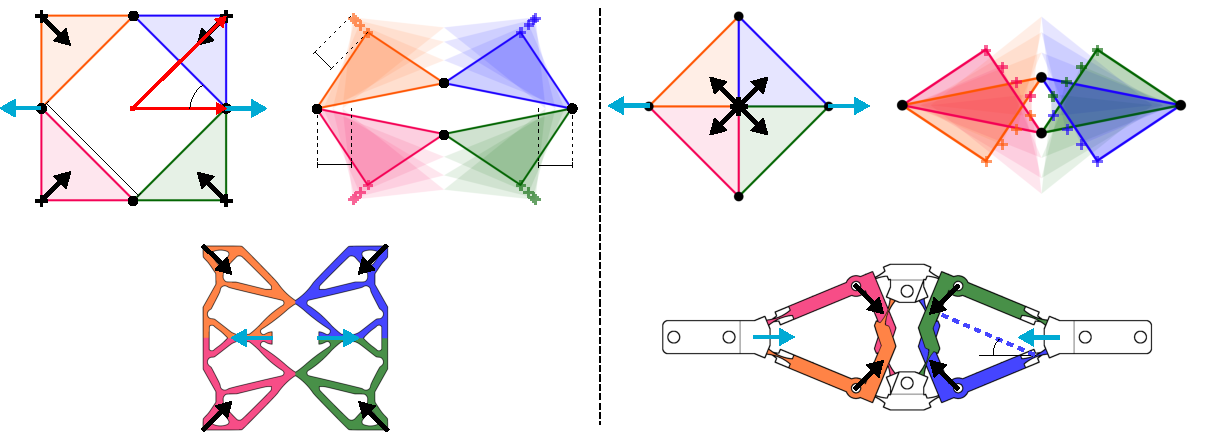
\includegraphics[width=\textwidth]{images/chap7/kinematic_schematics_models_reversed_legend_3.pdf}};
    \coordinate (ts0) at (\xLegendA,\yLegendTop); \node[align=left] at (ts0) {(a)};
    \coordinate (ts1) at (\xLegendB,\yLegendTop); \node[align=left] at (ts1) {(b)};
    \coordinate (ts2) at (\xLegendC,\yLegendTop); \node[align=left] at (ts2) {(c)};
    \coordinate (ts3) at (\xLegendD,\yLegendTop); \node[align=left] at (ts3) {(d)};
    \coordinate (ts4) at (\xLegendE,\yLegendBottom); \node[align=left] at (ts4) {(e)};
    \coordinate (ts5) at (\xLegendF,\yLegendBottom); \node[align=left] at (ts5) {(f)};

    %%%%%%%%%%%%%%%%%%%%%%%%%%%%%%%%%%%%%
    \node[align=left] at (\xLegendA+0.6,\yLegendTop+1.7) {$\theta$};
% 		\node[align=left] at (\xLegendA+0.45,\yLegendTop+2.1) {$\theta$};
% 		\node[align=left] at (\xLegendA+1.8,\yLegendTop+1.) {$L_s$};
    \node[align=left] at (\xLegendA+0.55,\yLegendTop+1.18) {\color{red}$\frac{x}{2}$};
    \node[align=left,rotate=45] at (\xLegendA+0.25,\yLegendTop+2.0) {\small\color{red}$R$};
    \node[align=left,rotate=-44] at (\xLegendA-0.2,\yLegendTop+1.0) {$L_h$};

    \node[align=left] at (\xLegendB+1.3,\yLegendTop+0.4) {$\frac{\Delta x}{2}$};
    \node[align=left] at (\xLegendB-1.5,\yLegendTop+0.4) {$\frac{\Delta x}{2}$};
% 		\node[align=left,rotate=-45] at (\xLegendB-2.1,\yLegendTop+2.35) {\small$R(\Delta x)$};
    \node[align=left,rotate=-45] at (\xLegendB-1.8,\yLegendTop+1.85) {\small$\Delta R$};

    \node[align=left] at (\xLegendF+0.55,\yLegendBottom+1.35) {$\theta_0$};
    % \draw[help lines] (0,0) grid (16,4); % $$$$$$$$$$$$$ HELPS A LOT FOR COORDINATES $$$$$$$
\end{tikzpicture}
\end{document}
}
  \caption{Kinematic diagram of proposed design where the black dots represent ideal pivots, the blue and black arrows represent the input and output displacement, respectively. On the left: the outward-triangle configuration with a) the initial position and b) the displaced one. On the right-hand side: the inward-triangle configuration achieving a stroke amplification with c) the initial position and d) the displaced one. e) represents mandrel topology generated with 2D topology optimization which behaves similarly to the outward version. f) shows the 2.5D adaptation of the inward version into a flexure-based mechanism distributed over multiple layers, and with a reversed actuation direction.}
  \label{fig:mandrel-kinematic}
\end{figure}

When examining the concept behind the mandrel mechanism, the conclusion can be made that the driving structure consists of four right-angled isosceles triangles which represent the four claws of the mandrel. Furthermore, the pivots, being constrained along the horizontal and vertical axes due to symmetry, force the outputs to move along a $45^{\circ}$ path. However, upon careful examination, these constraints can be satisfied in two distinct configurations as shown in \cref{fig:mandrel-kinematic}(a) and (c). The four triangles can be position inwardly or outwardly. Due to the inward-facing configuration having overlapping triangles, this topology cannot be generated from a 2D design space. The main advantage of the inward-facing configuration compared to the outward-facing configuration is the stroke amplification of the output vertices based on the stroke of the SMA coil contraction. It is also important to note that the direction of the radial output depends on the direction of the input displacement. Thus, the gripper can be made to open or close when the SMA coil is heated. By attaching the SMA coil to the vertical pivots rather than the horizontal ones, the gripper can be made to be always opened or always closed.

\subsubsection{Determining the Relationship between the Hinges and the SMA Stroke}
The stroke amplification, $\gamma$, of the system is not uniform and is dependant on the position of the mechanism, $x$. This amplification factor can be described by deriving the output vertex position, $R$, with respect to the input vertex position, $x$, and can be expressed analytically as :
\begin{equation}
\gamma(x) = \frac{\partial R(x)}{\partial x} = \frac{1}{2\sqrt{2}}\left(1-\text{sign}(\alpha)\frac{\frac{x}{2}}{\sqrt{L_{h}^2-\left(\frac{x}{2}\right)^2}} \right)
\label{eq:1}
\end{equation}
where,
\begin{equation}
\begin{split}
    R(x) &= L_{h}\cos\left(\theta(x) - \alpha\right)\\
     &= \frac{1}{\sqrt{2}} \left(\frac{x}{2} +\text{sign}(\alpha) \sqrt{L_{h}^2-\left(\frac{x}{2}\right)^2}\right),
    \label{eq:7}
\end{split}
\end{equation}
with,
\begin{equation}
\theta(x) = \arccos{\left(\frac{x}{2L_{h}}\right)} \quad \text{and} \quad \alpha=\pm\frac{\pi}{4}.
\label{eq:theta}
\end{equation}
Here, $L_h$ represents the length of the hypotenuse of each triangle, $\theta$ represents the angle between the horizontal and the hypotenuse, $\alpha$ represents the angle between the hypotenuse and the side of the triangle and can equal a value of $\pm\frac{\pi}{4}$. This angle is defined as positive for the outward-facing configuration and as negative for the inward-facing one. Here, the output stroke is majorly dependant on the sign of the angle $\alpha$. The outward configuration has a stroke amplification of less than one for almost all possible inputs, implying a stroke reduction. While, on the other hand, the inward configuration has a stroke amplification large than one. In the context of a gripper, the inward version was chosen for its larger output stroke.

\subsubsection{Simple Kinematics to a Compliant Mechanism}
The kinematic schematic is composed of only simple hinges and rigid links. This makes it the ideal candidate for implementation using flexure-based hinges. In this case, as shown in \cref{fig:mech_stages}, truncated semi-circular flexure hinges were selected for their ability to avoid high localised stress concentration and allow for an acceptable angular stroke as displayed in the work by \todocite.

\begin{figure}[hbt!] % t for top of the page, H could be put to impose the position of the float
  \centering
  \resizebox{0.9\textwidth}{!}{% !TEX root = ../sethomas_thesis_main.tex
\documentclass[border=1mm,
               class=article
               preview]{standalone}
\usepackage{tikz}
\begin{document}
\begin{tikzpicture}
    \pgfmathsetmacro{\YDelta}{1.1};%Offset for adding the side view

    \pgfmathsetmacro{\xLegendTop}{0.2};
    \pgfmathsetmacro{\yLegendTop}{5.3+\YDelta};

    \pgfmathsetmacro{\xLegendBottom}{1.1}; \pgfmathsetmacro{\yLegendBottom}{2.6+\YDelta};

    \pgfmathsetmacro{\xLegendSide}{0.2}; \pgfmathsetmacro{\yLegendSide}{0.65}

    % \node[anchor=south west,inner sep=0] (graph) at (0,0){\includegraphics[width=0.4\textwidth]{img/mechanism_iso_axes.png}};
    \node[anchor=south west,inner sep=0] (graph) at (0,0){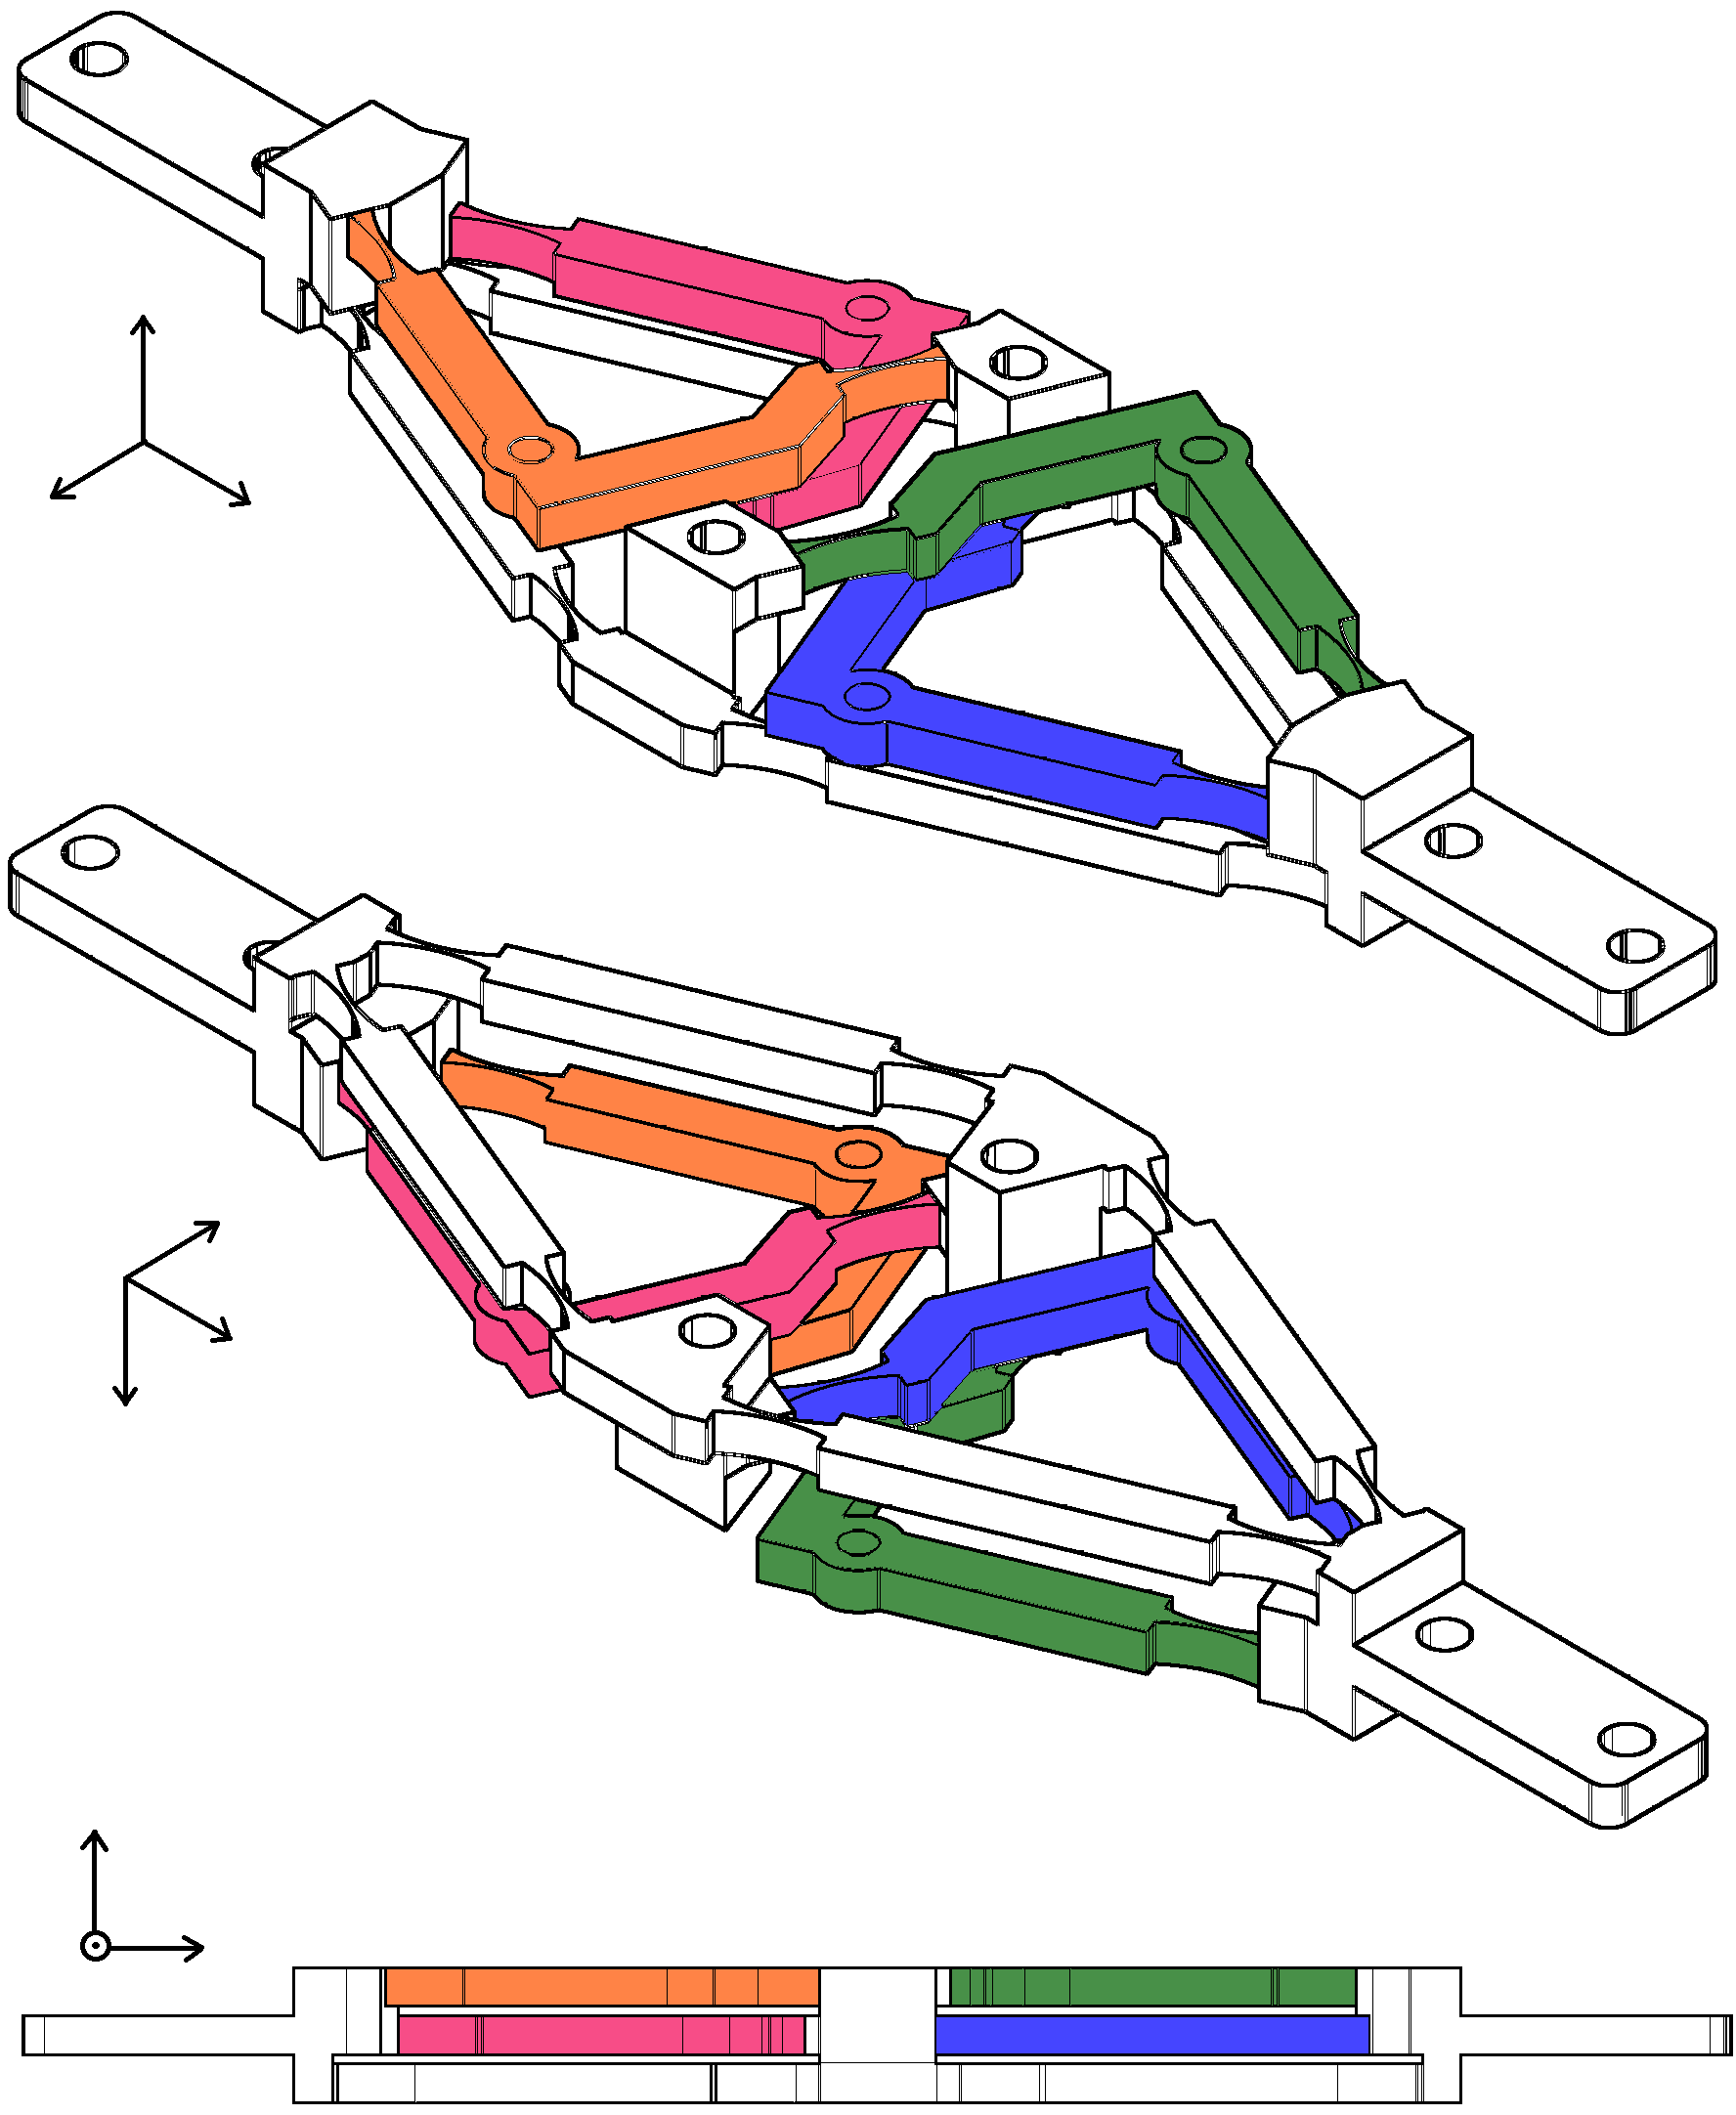
\includegraphics[width=0.4\textwidth]{images/chap7/mechanism_iso_axes_side.png}};
    \begin{scope}[x={(graph.south east)},y={(graph.north west)}]
        \node[align=left] at (0.04,0.742) {\footnotesize x};
        \node[align=left] at (0.15,0.735) {\footnotesize y};
        \node[align=left] at (0.06,0.85) {\footnotesize z};

        \node[align=left] at (0.095,0.445) {\footnotesize x};
        \node[align=left] at (0.155,0.345) {\footnotesize y};
        \node[align=left] at (0.045,0.34) {\footnotesize z};

        \node[align=left] at (0.03,0.1) {\footnotesize x};
        \node[align=left] at (0.135,0.1) {\footnotesize y};
        \node[align=left] at (0.08,0.155) {\footnotesize z};
    \end{scope}

    \pgfmathsetmacro{\xStartLine}{\xLegendSide-0.2};
    \pgfmathsetmacro{\xStopLine}{\xLegendSide+7};
    \draw[densely dotted] (\xStartLine,\yLegendSide-0.17) -- (\xStopLine,\yLegendSide-0.17);
    \node[align=left] at (\xStopLine+0.3,\yLegendSide-0.14) {\small $L_1$};
    \draw[densely dotted] (\xStartLine,\yLegendSide-0.37) -- (\xStopLine,\yLegendSide-0.37);
    \node[align=right] at (\xStartLine-0.3,\yLegendSide-0.34) {\small $L_2$}; %,draw,circle,inner sep=0.1pt
    \draw[densely dotted] (\xStartLine,\yLegendSide-0.57) -- (\xStopLine,\yLegendSide-0.57);
    \node[align=left] at (\xStopLine+0.3,\yLegendSide-0.6) {\small $L_3$};

    \pgfmathsetmacro{\xZOOM}{7.4};
    \pgfmathsetmacro{\yZOOM}{7.2};
    \node[anchor=north east,inner sep=0] (graph) at (\xZOOM,\yZOOM){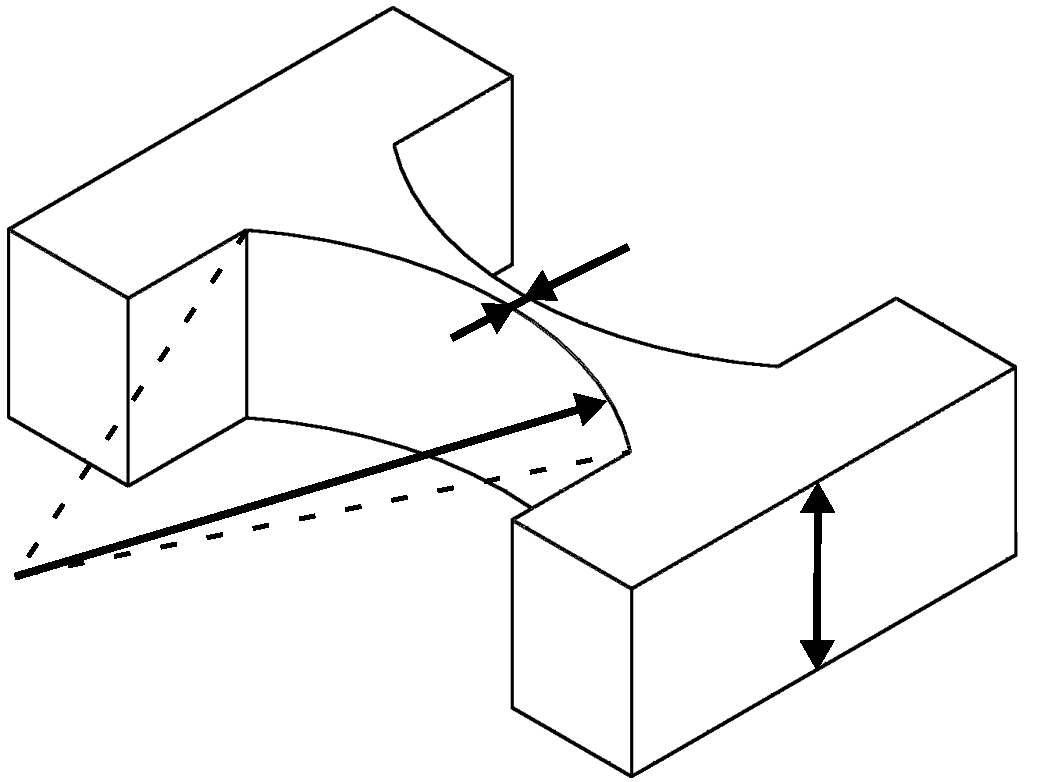
\includegraphics[width=2.5cm]{images/chap7/pivot.pdf}};
    \node[align=left] at (\xZOOM-1.,\yZOOM-0.45) {$e$};
    \node[align=left] at (\xZOOM-0.4,\yZOOM-1.3) {$b$};
    \node[align=left] at (\xZOOM-1.7,\yZOOM-1) {$r$};
    % \draw[help lines] (0,0) grid (8,8); % $$$$$$$$$$$$$ HELPS A LOT FOR COORDINATES $$$$$$$
\end{tikzpicture}
\end{document}
}
  \caption{Different views of the flexure-based compliant mechanism spreading over multiple stages, and parametrized flexure pivot.}
  \label{fig:mech_stages}
\end{figure}

As stated earlier, the inward-facing triangle configuration was chosen and due to fact that the triangles overlap during actuation, it makes it impossible to be implemented in a 2D design space. Thus, as shown in \cref{fig:mech_stages}, a 2.D design approach was implemented where each overlapping triangle is stacked in the 3\textsuperscript{rd} dimension. The mechanism is distributed among different superimposed layers linked at the vertices of the triangle to replicated the kinematic schematic. This adaptation to 2.5D design does not impact the functionality of the mechanism as long as the hinges are considered infinitely rigid when bending in any other direction other than the desired one. Here, two layers are implemented to accommodate the four triangles : the $L_1$ stage comprising of the green and orange triangles, and the $L_2$ stage comprising of the pink and blue triangles.

In the case of the ideal kinematic schematic, the triangles are attached at a single point to form a parallelogram. However, this is difficult to implement with a flexure-based solution due to the rigid links having a non-null width. This adds unwanted links and hinges to the kinematic chain which results in undesired Degrees of Freedom (DoF). This parasitic DoF is overcome by adding a third DoF-inhibiting stage, $L_3$, to the 2.5D design as shown in \cref{fig:mech_stages}.

As the goal of this gripper is for drone delivery purposes, another stage, which behaves as the frame of the drone, can be added to the design. For mechanism to behave as intended in the kinematic schematic, the left and right input vertices must be constraint to move along a single line. In this case, for simplicity, this constraint has been implemented using a rail. For a future drone mounted setup, an additional stage can be added to perform this required constraint, showing the advantage of the 2.5D design approach.

\subsubsection{Sizing of the Biasing Compliant Mechanism}
Based on the proposed design methodology, the goal of the mechanism is to create a kinematic stage that also behaves as the passive biasing element for the SMA coil. The inherent stiffness of the overall compliant mechanism due to the flexural hinges is harness to prestretch the SMA for activation. Thus, in order to size the actuator and the corresponding biasing element, an analytical model of the stiffness must be developed. Using the pseudo-rigid model, as presented in the work by \cite{heneinConceptionStructuresArticulees2005}, the flexural hinges can be considered as torsional spring with a constant angular stiffness, $K_\theta$. As detailed in \cref{subsec:passive-biasing-compliant-mech}, the stiffness of the compliant structure requires an expression for the relationship between angular position of the flexural hinge and the contraction of the SMA, $\theta(\Delta x)$. In this case, this relationship can be expressed as :
\begin{equation}\label{eq:mandrel-theta-model}
\theta(\Delta x) = \arccos{\left(\frac{\Delta x}{2L_{h}} + \cos(\theta_0)\right)},
\end{equation}
with $\theta_0$ being the resting angle at which the mechanism is printer/fabricated as shown in \cref{fig:mandrel-kinematic}(f).

As detailed in the methodology, the next step is to calculate the potential energy within the system during deformation. Due to the symmetry of the mechanism, all the hinges store the same potential energy. Here, the $L_3$ stage has 8 hinges while the stages $L_1$ and $L_2$ have 4 hinges each. Thus, the total potential energy of the whole mechanism is :
\begin{equation}\label{eq:mandrel-potential-energy-model}
U_\mathrm{tot}(\Delta x) = 16\cdot U(\Delta x)
\end{equation}
The force-displacement characteristic of the mechanism is then given by :
\begin{equation}\label{eq:mandrel-force-model}
\begin{split}
    F(\Delta x) &= \lVert -\nabla{U_\text{tot}(\Delta x)}\rVert = \frac{\partial U_\text{tot}(\Delta x)}{\partial \Delta x}\\
     &= \frac{8K_{\theta}}{L_{h}}  \frac{(\theta(\Delta x)-\theta_{0})}{\sin(\theta(\Delta x))}.
\end{split}
\end{equation}
The resulting characteristic is plotted as shown in \cref{fig:mandrel-am-expt-compare}. Furthermore, the model is validated using experimental results obtained using a pull-tester. As the experimental results follow the model quite closely, it validates the working hypothesis and approximations used during the definition of the analytical model.
\begin{figure}[hbt!] % t for top of the page, H could be put to impose the position of the float
  \centering
  \resizebox{0.9\textwidth}{!}{%% Creator: Matplotlib, PGF backend
%%
%% To include the figure in your LaTeX document, write
%%   \input{<filename>.pgf}
%%
%% Make sure the required packages are loaded in your preamble
%%   \usepackage{pgf}
%%
%% and, on pdftex
%%   \usepackage[utf8]{inputenc}\DeclareUnicodeCharacter{2212}{-}
%%
%% or, on luatex and xetex
%%   \usepackage{unicode-math}
%%
%% Figures using additional raster images can only be included by \input if
%% they are in the same directory as the main LaTeX file. For loading figures
%% from other directories you can use the `import` package
%%   \usepackage{import}
%%
%% and then include the figures with
%%   \import{<path to file>}{<filename>.pgf}
%%
%% Matplotlib used the following preamble
%%
\begingroup%
\makeatletter%
\begin{pgfpicture}%
\pgfpathrectangle{\pgfpointorigin}{\pgfqpoint{9.500000in}{4.700000in}}%
\pgfusepath{use as bounding box, clip}%
\begin{pgfscope}%
\pgfsetbuttcap%
\pgfsetmiterjoin%
\pgfsetlinewidth{0.000000pt}%
\definecolor{currentstroke}{rgb}{0.000000,0.000000,0.000000}%
\pgfsetstrokecolor{currentstroke}%
\pgfsetstrokeopacity{0.000000}%
\pgfsetdash{}{0pt}%
\pgfpathmoveto{\pgfqpoint{0.000000in}{-0.000000in}}%
\pgfpathlineto{\pgfqpoint{9.500000in}{-0.000000in}}%
\pgfpathlineto{\pgfqpoint{9.500000in}{4.700000in}}%
\pgfpathlineto{\pgfqpoint{0.000000in}{4.700000in}}%
\pgfpathclose%
\pgfusepath{}%
\end{pgfscope}%
\begin{pgfscope}%
\pgfsetbuttcap%
\pgfsetmiterjoin%
\pgfsetlinewidth{0.000000pt}%
\definecolor{currentstroke}{rgb}{0.000000,0.000000,0.000000}%
\pgfsetstrokecolor{currentstroke}%
\pgfsetstrokeopacity{0.000000}%
\pgfsetdash{}{0pt}%
\pgfpathmoveto{\pgfqpoint{0.898145in}{0.670138in}}%
\pgfpathlineto{\pgfqpoint{9.400000in}{0.670138in}}%
\pgfpathlineto{\pgfqpoint{9.400000in}{4.600000in}}%
\pgfpathlineto{\pgfqpoint{0.898145in}{4.600000in}}%
\pgfpathclose%
\pgfusepath{}%
\end{pgfscope}%
\begin{pgfscope}%
\pgfpathrectangle{\pgfqpoint{0.898145in}{0.670138in}}{\pgfqpoint{8.501855in}{3.929862in}}%
\pgfusepath{clip}%
\pgfsetrectcap%
\pgfsetroundjoin%
\pgfsetlinewidth{0.803000pt}%
\definecolor{currentstroke}{rgb}{0.690196,0.690196,0.690196}%
\pgfsetstrokecolor{currentstroke}%
\pgfsetstrokeopacity{0.200000}%
\pgfsetdash{}{0pt}%
\pgfpathmoveto{\pgfqpoint{1.284593in}{0.670138in}}%
\pgfpathlineto{\pgfqpoint{1.284593in}{4.600000in}}%
\pgfusepath{stroke}%
\end{pgfscope}%
\begin{pgfscope}%
\pgfsetbuttcap%
\pgfsetroundjoin%
\definecolor{currentfill}{rgb}{0.000000,0.000000,0.000000}%
\pgfsetfillcolor{currentfill}%
\pgfsetlinewidth{0.803000pt}%
\definecolor{currentstroke}{rgb}{0.000000,0.000000,0.000000}%
\pgfsetstrokecolor{currentstroke}%
\pgfsetdash{}{0pt}%
\pgfsys@defobject{currentmarker}{\pgfqpoint{0.000000in}{-0.048611in}}{\pgfqpoint{0.000000in}{0.000000in}}{%
\pgfpathmoveto{\pgfqpoint{0.000000in}{0.000000in}}%
\pgfpathlineto{\pgfqpoint{0.000000in}{-0.048611in}}%
\pgfusepath{stroke,fill}%
}%
\begin{pgfscope}%
\pgfsys@transformshift{1.284593in}{0.670138in}%
\pgfsys@useobject{currentmarker}{}%
\end{pgfscope}%
\end{pgfscope}%
\begin{pgfscope}%
\definecolor{textcolor}{rgb}{0.000000,0.000000,0.000000}%
\pgfsetstrokecolor{textcolor}%
\pgfsetfillcolor{textcolor}%
\pgftext[x=1.284593in,y=0.572916in,,top]{\color{textcolor}\rmfamily\fontsize{14.000000}{16.800000}\selectfont \(\displaystyle {-6}\)}%
\end{pgfscope}%
\begin{pgfscope}%
\pgfpathrectangle{\pgfqpoint{0.898145in}{0.670138in}}{\pgfqpoint{8.501855in}{3.929862in}}%
\pgfusepath{clip}%
\pgfsetrectcap%
\pgfsetroundjoin%
\pgfsetlinewidth{0.803000pt}%
\definecolor{currentstroke}{rgb}{0.690196,0.690196,0.690196}%
\pgfsetstrokecolor{currentstroke}%
\pgfsetstrokeopacity{0.200000}%
\pgfsetdash{}{0pt}%
\pgfpathmoveto{\pgfqpoint{2.057489in}{0.670138in}}%
\pgfpathlineto{\pgfqpoint{2.057489in}{4.600000in}}%
\pgfusepath{stroke}%
\end{pgfscope}%
\begin{pgfscope}%
\pgfsetbuttcap%
\pgfsetroundjoin%
\definecolor{currentfill}{rgb}{0.000000,0.000000,0.000000}%
\pgfsetfillcolor{currentfill}%
\pgfsetlinewidth{0.803000pt}%
\definecolor{currentstroke}{rgb}{0.000000,0.000000,0.000000}%
\pgfsetstrokecolor{currentstroke}%
\pgfsetdash{}{0pt}%
\pgfsys@defobject{currentmarker}{\pgfqpoint{0.000000in}{-0.048611in}}{\pgfqpoint{0.000000in}{0.000000in}}{%
\pgfpathmoveto{\pgfqpoint{0.000000in}{0.000000in}}%
\pgfpathlineto{\pgfqpoint{0.000000in}{-0.048611in}}%
\pgfusepath{stroke,fill}%
}%
\begin{pgfscope}%
\pgfsys@transformshift{2.057489in}{0.670138in}%
\pgfsys@useobject{currentmarker}{}%
\end{pgfscope}%
\end{pgfscope}%
\begin{pgfscope}%
\definecolor{textcolor}{rgb}{0.000000,0.000000,0.000000}%
\pgfsetstrokecolor{textcolor}%
\pgfsetfillcolor{textcolor}%
\pgftext[x=2.057489in,y=0.572916in,,top]{\color{textcolor}\rmfamily\fontsize{14.000000}{16.800000}\selectfont \(\displaystyle {-5}\)}%
\end{pgfscope}%
\begin{pgfscope}%
\pgfpathrectangle{\pgfqpoint{0.898145in}{0.670138in}}{\pgfqpoint{8.501855in}{3.929862in}}%
\pgfusepath{clip}%
\pgfsetrectcap%
\pgfsetroundjoin%
\pgfsetlinewidth{0.803000pt}%
\definecolor{currentstroke}{rgb}{0.690196,0.690196,0.690196}%
\pgfsetstrokecolor{currentstroke}%
\pgfsetstrokeopacity{0.200000}%
\pgfsetdash{}{0pt}%
\pgfpathmoveto{\pgfqpoint{2.830385in}{0.670138in}}%
\pgfpathlineto{\pgfqpoint{2.830385in}{4.600000in}}%
\pgfusepath{stroke}%
\end{pgfscope}%
\begin{pgfscope}%
\pgfsetbuttcap%
\pgfsetroundjoin%
\definecolor{currentfill}{rgb}{0.000000,0.000000,0.000000}%
\pgfsetfillcolor{currentfill}%
\pgfsetlinewidth{0.803000pt}%
\definecolor{currentstroke}{rgb}{0.000000,0.000000,0.000000}%
\pgfsetstrokecolor{currentstroke}%
\pgfsetdash{}{0pt}%
\pgfsys@defobject{currentmarker}{\pgfqpoint{0.000000in}{-0.048611in}}{\pgfqpoint{0.000000in}{0.000000in}}{%
\pgfpathmoveto{\pgfqpoint{0.000000in}{0.000000in}}%
\pgfpathlineto{\pgfqpoint{0.000000in}{-0.048611in}}%
\pgfusepath{stroke,fill}%
}%
\begin{pgfscope}%
\pgfsys@transformshift{2.830385in}{0.670138in}%
\pgfsys@useobject{currentmarker}{}%
\end{pgfscope}%
\end{pgfscope}%
\begin{pgfscope}%
\definecolor{textcolor}{rgb}{0.000000,0.000000,0.000000}%
\pgfsetstrokecolor{textcolor}%
\pgfsetfillcolor{textcolor}%
\pgftext[x=2.830385in,y=0.572916in,,top]{\color{textcolor}\rmfamily\fontsize{14.000000}{16.800000}\selectfont \(\displaystyle {-4}\)}%
\end{pgfscope}%
\begin{pgfscope}%
\pgfpathrectangle{\pgfqpoint{0.898145in}{0.670138in}}{\pgfqpoint{8.501855in}{3.929862in}}%
\pgfusepath{clip}%
\pgfsetrectcap%
\pgfsetroundjoin%
\pgfsetlinewidth{0.803000pt}%
\definecolor{currentstroke}{rgb}{0.690196,0.690196,0.690196}%
\pgfsetstrokecolor{currentstroke}%
\pgfsetstrokeopacity{0.200000}%
\pgfsetdash{}{0pt}%
\pgfpathmoveto{\pgfqpoint{3.603281in}{0.670138in}}%
\pgfpathlineto{\pgfqpoint{3.603281in}{4.600000in}}%
\pgfusepath{stroke}%
\end{pgfscope}%
\begin{pgfscope}%
\pgfsetbuttcap%
\pgfsetroundjoin%
\definecolor{currentfill}{rgb}{0.000000,0.000000,0.000000}%
\pgfsetfillcolor{currentfill}%
\pgfsetlinewidth{0.803000pt}%
\definecolor{currentstroke}{rgb}{0.000000,0.000000,0.000000}%
\pgfsetstrokecolor{currentstroke}%
\pgfsetdash{}{0pt}%
\pgfsys@defobject{currentmarker}{\pgfqpoint{0.000000in}{-0.048611in}}{\pgfqpoint{0.000000in}{0.000000in}}{%
\pgfpathmoveto{\pgfqpoint{0.000000in}{0.000000in}}%
\pgfpathlineto{\pgfqpoint{0.000000in}{-0.048611in}}%
\pgfusepath{stroke,fill}%
}%
\begin{pgfscope}%
\pgfsys@transformshift{3.603281in}{0.670138in}%
\pgfsys@useobject{currentmarker}{}%
\end{pgfscope}%
\end{pgfscope}%
\begin{pgfscope}%
\definecolor{textcolor}{rgb}{0.000000,0.000000,0.000000}%
\pgfsetstrokecolor{textcolor}%
\pgfsetfillcolor{textcolor}%
\pgftext[x=3.603281in,y=0.572916in,,top]{\color{textcolor}\rmfamily\fontsize{14.000000}{16.800000}\selectfont \(\displaystyle {-3}\)}%
\end{pgfscope}%
\begin{pgfscope}%
\pgfpathrectangle{\pgfqpoint{0.898145in}{0.670138in}}{\pgfqpoint{8.501855in}{3.929862in}}%
\pgfusepath{clip}%
\pgfsetrectcap%
\pgfsetroundjoin%
\pgfsetlinewidth{0.803000pt}%
\definecolor{currentstroke}{rgb}{0.690196,0.690196,0.690196}%
\pgfsetstrokecolor{currentstroke}%
\pgfsetstrokeopacity{0.200000}%
\pgfsetdash{}{0pt}%
\pgfpathmoveto{\pgfqpoint{4.376177in}{0.670138in}}%
\pgfpathlineto{\pgfqpoint{4.376177in}{4.600000in}}%
\pgfusepath{stroke}%
\end{pgfscope}%
\begin{pgfscope}%
\pgfsetbuttcap%
\pgfsetroundjoin%
\definecolor{currentfill}{rgb}{0.000000,0.000000,0.000000}%
\pgfsetfillcolor{currentfill}%
\pgfsetlinewidth{0.803000pt}%
\definecolor{currentstroke}{rgb}{0.000000,0.000000,0.000000}%
\pgfsetstrokecolor{currentstroke}%
\pgfsetdash{}{0pt}%
\pgfsys@defobject{currentmarker}{\pgfqpoint{0.000000in}{-0.048611in}}{\pgfqpoint{0.000000in}{0.000000in}}{%
\pgfpathmoveto{\pgfqpoint{0.000000in}{0.000000in}}%
\pgfpathlineto{\pgfqpoint{0.000000in}{-0.048611in}}%
\pgfusepath{stroke,fill}%
}%
\begin{pgfscope}%
\pgfsys@transformshift{4.376177in}{0.670138in}%
\pgfsys@useobject{currentmarker}{}%
\end{pgfscope}%
\end{pgfscope}%
\begin{pgfscope}%
\definecolor{textcolor}{rgb}{0.000000,0.000000,0.000000}%
\pgfsetstrokecolor{textcolor}%
\pgfsetfillcolor{textcolor}%
\pgftext[x=4.376177in,y=0.572916in,,top]{\color{textcolor}\rmfamily\fontsize{14.000000}{16.800000}\selectfont \(\displaystyle {-2}\)}%
\end{pgfscope}%
\begin{pgfscope}%
\pgfpathrectangle{\pgfqpoint{0.898145in}{0.670138in}}{\pgfqpoint{8.501855in}{3.929862in}}%
\pgfusepath{clip}%
\pgfsetrectcap%
\pgfsetroundjoin%
\pgfsetlinewidth{0.803000pt}%
\definecolor{currentstroke}{rgb}{0.690196,0.690196,0.690196}%
\pgfsetstrokecolor{currentstroke}%
\pgfsetstrokeopacity{0.200000}%
\pgfsetdash{}{0pt}%
\pgfpathmoveto{\pgfqpoint{5.149072in}{0.670138in}}%
\pgfpathlineto{\pgfqpoint{5.149072in}{4.600000in}}%
\pgfusepath{stroke}%
\end{pgfscope}%
\begin{pgfscope}%
\pgfsetbuttcap%
\pgfsetroundjoin%
\definecolor{currentfill}{rgb}{0.000000,0.000000,0.000000}%
\pgfsetfillcolor{currentfill}%
\pgfsetlinewidth{0.803000pt}%
\definecolor{currentstroke}{rgb}{0.000000,0.000000,0.000000}%
\pgfsetstrokecolor{currentstroke}%
\pgfsetdash{}{0pt}%
\pgfsys@defobject{currentmarker}{\pgfqpoint{0.000000in}{-0.048611in}}{\pgfqpoint{0.000000in}{0.000000in}}{%
\pgfpathmoveto{\pgfqpoint{0.000000in}{0.000000in}}%
\pgfpathlineto{\pgfqpoint{0.000000in}{-0.048611in}}%
\pgfusepath{stroke,fill}%
}%
\begin{pgfscope}%
\pgfsys@transformshift{5.149072in}{0.670138in}%
\pgfsys@useobject{currentmarker}{}%
\end{pgfscope}%
\end{pgfscope}%
\begin{pgfscope}%
\definecolor{textcolor}{rgb}{0.000000,0.000000,0.000000}%
\pgfsetstrokecolor{textcolor}%
\pgfsetfillcolor{textcolor}%
\pgftext[x=5.149072in,y=0.572916in,,top]{\color{textcolor}\rmfamily\fontsize{14.000000}{16.800000}\selectfont \(\displaystyle {-1}\)}%
\end{pgfscope}%
\begin{pgfscope}%
\pgfpathrectangle{\pgfqpoint{0.898145in}{0.670138in}}{\pgfqpoint{8.501855in}{3.929862in}}%
\pgfusepath{clip}%
\pgfsetrectcap%
\pgfsetroundjoin%
\pgfsetlinewidth{0.803000pt}%
\definecolor{currentstroke}{rgb}{0.690196,0.690196,0.690196}%
\pgfsetstrokecolor{currentstroke}%
\pgfsetstrokeopacity{0.200000}%
\pgfsetdash{}{0pt}%
\pgfpathmoveto{\pgfqpoint{5.921968in}{0.670138in}}%
\pgfpathlineto{\pgfqpoint{5.921968in}{4.600000in}}%
\pgfusepath{stroke}%
\end{pgfscope}%
\begin{pgfscope}%
\pgfsetbuttcap%
\pgfsetroundjoin%
\definecolor{currentfill}{rgb}{0.000000,0.000000,0.000000}%
\pgfsetfillcolor{currentfill}%
\pgfsetlinewidth{0.803000pt}%
\definecolor{currentstroke}{rgb}{0.000000,0.000000,0.000000}%
\pgfsetstrokecolor{currentstroke}%
\pgfsetdash{}{0pt}%
\pgfsys@defobject{currentmarker}{\pgfqpoint{0.000000in}{-0.048611in}}{\pgfqpoint{0.000000in}{0.000000in}}{%
\pgfpathmoveto{\pgfqpoint{0.000000in}{0.000000in}}%
\pgfpathlineto{\pgfqpoint{0.000000in}{-0.048611in}}%
\pgfusepath{stroke,fill}%
}%
\begin{pgfscope}%
\pgfsys@transformshift{5.921968in}{0.670138in}%
\pgfsys@useobject{currentmarker}{}%
\end{pgfscope}%
\end{pgfscope}%
\begin{pgfscope}%
\definecolor{textcolor}{rgb}{0.000000,0.000000,0.000000}%
\pgfsetstrokecolor{textcolor}%
\pgfsetfillcolor{textcolor}%
\pgftext[x=5.921968in,y=0.572916in,,top]{\color{textcolor}\rmfamily\fontsize{14.000000}{16.800000}\selectfont \(\displaystyle {0}\)}%
\end{pgfscope}%
\begin{pgfscope}%
\pgfpathrectangle{\pgfqpoint{0.898145in}{0.670138in}}{\pgfqpoint{8.501855in}{3.929862in}}%
\pgfusepath{clip}%
\pgfsetrectcap%
\pgfsetroundjoin%
\pgfsetlinewidth{0.803000pt}%
\definecolor{currentstroke}{rgb}{0.690196,0.690196,0.690196}%
\pgfsetstrokecolor{currentstroke}%
\pgfsetstrokeopacity{0.200000}%
\pgfsetdash{}{0pt}%
\pgfpathmoveto{\pgfqpoint{6.694864in}{0.670138in}}%
\pgfpathlineto{\pgfqpoint{6.694864in}{4.600000in}}%
\pgfusepath{stroke}%
\end{pgfscope}%
\begin{pgfscope}%
\pgfsetbuttcap%
\pgfsetroundjoin%
\definecolor{currentfill}{rgb}{0.000000,0.000000,0.000000}%
\pgfsetfillcolor{currentfill}%
\pgfsetlinewidth{0.803000pt}%
\definecolor{currentstroke}{rgb}{0.000000,0.000000,0.000000}%
\pgfsetstrokecolor{currentstroke}%
\pgfsetdash{}{0pt}%
\pgfsys@defobject{currentmarker}{\pgfqpoint{0.000000in}{-0.048611in}}{\pgfqpoint{0.000000in}{0.000000in}}{%
\pgfpathmoveto{\pgfqpoint{0.000000in}{0.000000in}}%
\pgfpathlineto{\pgfqpoint{0.000000in}{-0.048611in}}%
\pgfusepath{stroke,fill}%
}%
\begin{pgfscope}%
\pgfsys@transformshift{6.694864in}{0.670138in}%
\pgfsys@useobject{currentmarker}{}%
\end{pgfscope}%
\end{pgfscope}%
\begin{pgfscope}%
\definecolor{textcolor}{rgb}{0.000000,0.000000,0.000000}%
\pgfsetstrokecolor{textcolor}%
\pgfsetfillcolor{textcolor}%
\pgftext[x=6.694864in,y=0.572916in,,top]{\color{textcolor}\rmfamily\fontsize{14.000000}{16.800000}\selectfont \(\displaystyle {1}\)}%
\end{pgfscope}%
\begin{pgfscope}%
\pgfpathrectangle{\pgfqpoint{0.898145in}{0.670138in}}{\pgfqpoint{8.501855in}{3.929862in}}%
\pgfusepath{clip}%
\pgfsetrectcap%
\pgfsetroundjoin%
\pgfsetlinewidth{0.803000pt}%
\definecolor{currentstroke}{rgb}{0.690196,0.690196,0.690196}%
\pgfsetstrokecolor{currentstroke}%
\pgfsetstrokeopacity{0.200000}%
\pgfsetdash{}{0pt}%
\pgfpathmoveto{\pgfqpoint{7.467760in}{0.670138in}}%
\pgfpathlineto{\pgfqpoint{7.467760in}{4.600000in}}%
\pgfusepath{stroke}%
\end{pgfscope}%
\begin{pgfscope}%
\pgfsetbuttcap%
\pgfsetroundjoin%
\definecolor{currentfill}{rgb}{0.000000,0.000000,0.000000}%
\pgfsetfillcolor{currentfill}%
\pgfsetlinewidth{0.803000pt}%
\definecolor{currentstroke}{rgb}{0.000000,0.000000,0.000000}%
\pgfsetstrokecolor{currentstroke}%
\pgfsetdash{}{0pt}%
\pgfsys@defobject{currentmarker}{\pgfqpoint{0.000000in}{-0.048611in}}{\pgfqpoint{0.000000in}{0.000000in}}{%
\pgfpathmoveto{\pgfqpoint{0.000000in}{0.000000in}}%
\pgfpathlineto{\pgfqpoint{0.000000in}{-0.048611in}}%
\pgfusepath{stroke,fill}%
}%
\begin{pgfscope}%
\pgfsys@transformshift{7.467760in}{0.670138in}%
\pgfsys@useobject{currentmarker}{}%
\end{pgfscope}%
\end{pgfscope}%
\begin{pgfscope}%
\definecolor{textcolor}{rgb}{0.000000,0.000000,0.000000}%
\pgfsetstrokecolor{textcolor}%
\pgfsetfillcolor{textcolor}%
\pgftext[x=7.467760in,y=0.572916in,,top]{\color{textcolor}\rmfamily\fontsize{14.000000}{16.800000}\selectfont \(\displaystyle {2}\)}%
\end{pgfscope}%
\begin{pgfscope}%
\pgfpathrectangle{\pgfqpoint{0.898145in}{0.670138in}}{\pgfqpoint{8.501855in}{3.929862in}}%
\pgfusepath{clip}%
\pgfsetrectcap%
\pgfsetroundjoin%
\pgfsetlinewidth{0.803000pt}%
\definecolor{currentstroke}{rgb}{0.690196,0.690196,0.690196}%
\pgfsetstrokecolor{currentstroke}%
\pgfsetstrokeopacity{0.200000}%
\pgfsetdash{}{0pt}%
\pgfpathmoveto{\pgfqpoint{8.240656in}{0.670138in}}%
\pgfpathlineto{\pgfqpoint{8.240656in}{4.600000in}}%
\pgfusepath{stroke}%
\end{pgfscope}%
\begin{pgfscope}%
\pgfsetbuttcap%
\pgfsetroundjoin%
\definecolor{currentfill}{rgb}{0.000000,0.000000,0.000000}%
\pgfsetfillcolor{currentfill}%
\pgfsetlinewidth{0.803000pt}%
\definecolor{currentstroke}{rgb}{0.000000,0.000000,0.000000}%
\pgfsetstrokecolor{currentstroke}%
\pgfsetdash{}{0pt}%
\pgfsys@defobject{currentmarker}{\pgfqpoint{0.000000in}{-0.048611in}}{\pgfqpoint{0.000000in}{0.000000in}}{%
\pgfpathmoveto{\pgfqpoint{0.000000in}{0.000000in}}%
\pgfpathlineto{\pgfqpoint{0.000000in}{-0.048611in}}%
\pgfusepath{stroke,fill}%
}%
\begin{pgfscope}%
\pgfsys@transformshift{8.240656in}{0.670138in}%
\pgfsys@useobject{currentmarker}{}%
\end{pgfscope}%
\end{pgfscope}%
\begin{pgfscope}%
\definecolor{textcolor}{rgb}{0.000000,0.000000,0.000000}%
\pgfsetstrokecolor{textcolor}%
\pgfsetfillcolor{textcolor}%
\pgftext[x=8.240656in,y=0.572916in,,top]{\color{textcolor}\rmfamily\fontsize{14.000000}{16.800000}\selectfont \(\displaystyle {3}\)}%
\end{pgfscope}%
\begin{pgfscope}%
\pgfpathrectangle{\pgfqpoint{0.898145in}{0.670138in}}{\pgfqpoint{8.501855in}{3.929862in}}%
\pgfusepath{clip}%
\pgfsetrectcap%
\pgfsetroundjoin%
\pgfsetlinewidth{0.803000pt}%
\definecolor{currentstroke}{rgb}{0.690196,0.690196,0.690196}%
\pgfsetstrokecolor{currentstroke}%
\pgfsetstrokeopacity{0.200000}%
\pgfsetdash{}{0pt}%
\pgfpathmoveto{\pgfqpoint{9.013552in}{0.670138in}}%
\pgfpathlineto{\pgfqpoint{9.013552in}{4.600000in}}%
\pgfusepath{stroke}%
\end{pgfscope}%
\begin{pgfscope}%
\pgfsetbuttcap%
\pgfsetroundjoin%
\definecolor{currentfill}{rgb}{0.000000,0.000000,0.000000}%
\pgfsetfillcolor{currentfill}%
\pgfsetlinewidth{0.803000pt}%
\definecolor{currentstroke}{rgb}{0.000000,0.000000,0.000000}%
\pgfsetstrokecolor{currentstroke}%
\pgfsetdash{}{0pt}%
\pgfsys@defobject{currentmarker}{\pgfqpoint{0.000000in}{-0.048611in}}{\pgfqpoint{0.000000in}{0.000000in}}{%
\pgfpathmoveto{\pgfqpoint{0.000000in}{0.000000in}}%
\pgfpathlineto{\pgfqpoint{0.000000in}{-0.048611in}}%
\pgfusepath{stroke,fill}%
}%
\begin{pgfscope}%
\pgfsys@transformshift{9.013552in}{0.670138in}%
\pgfsys@useobject{currentmarker}{}%
\end{pgfscope}%
\end{pgfscope}%
\begin{pgfscope}%
\definecolor{textcolor}{rgb}{0.000000,0.000000,0.000000}%
\pgfsetstrokecolor{textcolor}%
\pgfsetfillcolor{textcolor}%
\pgftext[x=9.013552in,y=0.572916in,,top]{\color{textcolor}\rmfamily\fontsize{14.000000}{16.800000}\selectfont \(\displaystyle {4}\)}%
\end{pgfscope}%
\begin{pgfscope}%
\definecolor{textcolor}{rgb}{0.000000,0.000000,0.000000}%
\pgfsetstrokecolor{textcolor}%
\pgfsetfillcolor{textcolor}%
\pgftext[x=5.149072in,y=0.339583in,,top]{\color{textcolor}\rmfamily\fontsize{16.000000}{19.200000}\selectfont \textbf{Displacement [mm]}}%
\end{pgfscope}%
\begin{pgfscope}%
\pgfpathrectangle{\pgfqpoint{0.898145in}{0.670138in}}{\pgfqpoint{8.501855in}{3.929862in}}%
\pgfusepath{clip}%
\pgfsetrectcap%
\pgfsetroundjoin%
\pgfsetlinewidth{0.803000pt}%
\definecolor{currentstroke}{rgb}{0.690196,0.690196,0.690196}%
\pgfsetstrokecolor{currentstroke}%
\pgfsetstrokeopacity{0.200000}%
\pgfsetdash{}{0pt}%
\pgfpathmoveto{\pgfqpoint{0.898145in}{0.763706in}}%
\pgfpathlineto{\pgfqpoint{9.400000in}{0.763706in}}%
\pgfusepath{stroke}%
\end{pgfscope}%
\begin{pgfscope}%
\pgfsetbuttcap%
\pgfsetroundjoin%
\definecolor{currentfill}{rgb}{0.000000,0.000000,0.000000}%
\pgfsetfillcolor{currentfill}%
\pgfsetlinewidth{0.803000pt}%
\definecolor{currentstroke}{rgb}{0.000000,0.000000,0.000000}%
\pgfsetstrokecolor{currentstroke}%
\pgfsetdash{}{0pt}%
\pgfsys@defobject{currentmarker}{\pgfqpoint{-0.048611in}{0.000000in}}{\pgfqpoint{-0.000000in}{0.000000in}}{%
\pgfpathmoveto{\pgfqpoint{-0.000000in}{0.000000in}}%
\pgfpathlineto{\pgfqpoint{-0.048611in}{0.000000in}}%
\pgfusepath{stroke,fill}%
}%
\begin{pgfscope}%
\pgfsys@transformshift{0.898145in}{0.763706in}%
\pgfsys@useobject{currentmarker}{}%
\end{pgfscope}%
\end{pgfscope}%
\begin{pgfscope}%
\definecolor{textcolor}{rgb}{0.000000,0.000000,0.000000}%
\pgfsetstrokecolor{textcolor}%
\pgfsetfillcolor{textcolor}%
\pgftext[x=0.395138in, y=0.694262in, left, base]{\color{textcolor}\rmfamily\fontsize{14.000000}{16.800000}\selectfont \(\displaystyle {-2.5}\)}%
\end{pgfscope}%
\begin{pgfscope}%
\pgfpathrectangle{\pgfqpoint{0.898145in}{0.670138in}}{\pgfqpoint{8.501855in}{3.929862in}}%
\pgfusepath{clip}%
\pgfsetrectcap%
\pgfsetroundjoin%
\pgfsetlinewidth{0.803000pt}%
\definecolor{currentstroke}{rgb}{0.690196,0.690196,0.690196}%
\pgfsetstrokecolor{currentstroke}%
\pgfsetstrokeopacity{0.200000}%
\pgfsetdash{}{0pt}%
\pgfpathmoveto{\pgfqpoint{0.898145in}{1.231547in}}%
\pgfpathlineto{\pgfqpoint{9.400000in}{1.231547in}}%
\pgfusepath{stroke}%
\end{pgfscope}%
\begin{pgfscope}%
\pgfsetbuttcap%
\pgfsetroundjoin%
\definecolor{currentfill}{rgb}{0.000000,0.000000,0.000000}%
\pgfsetfillcolor{currentfill}%
\pgfsetlinewidth{0.803000pt}%
\definecolor{currentstroke}{rgb}{0.000000,0.000000,0.000000}%
\pgfsetstrokecolor{currentstroke}%
\pgfsetdash{}{0pt}%
\pgfsys@defobject{currentmarker}{\pgfqpoint{-0.048611in}{0.000000in}}{\pgfqpoint{-0.000000in}{0.000000in}}{%
\pgfpathmoveto{\pgfqpoint{-0.000000in}{0.000000in}}%
\pgfpathlineto{\pgfqpoint{-0.048611in}{0.000000in}}%
\pgfusepath{stroke,fill}%
}%
\begin{pgfscope}%
\pgfsys@transformshift{0.898145in}{1.231547in}%
\pgfsys@useobject{currentmarker}{}%
\end{pgfscope}%
\end{pgfscope}%
\begin{pgfscope}%
\definecolor{textcolor}{rgb}{0.000000,0.000000,0.000000}%
\pgfsetstrokecolor{textcolor}%
\pgfsetfillcolor{textcolor}%
\pgftext[x=0.395138in, y=1.162103in, left, base]{\color{textcolor}\rmfamily\fontsize{14.000000}{16.800000}\selectfont \(\displaystyle {-2.0}\)}%
\end{pgfscope}%
\begin{pgfscope}%
\pgfpathrectangle{\pgfqpoint{0.898145in}{0.670138in}}{\pgfqpoint{8.501855in}{3.929862in}}%
\pgfusepath{clip}%
\pgfsetrectcap%
\pgfsetroundjoin%
\pgfsetlinewidth{0.803000pt}%
\definecolor{currentstroke}{rgb}{0.690196,0.690196,0.690196}%
\pgfsetstrokecolor{currentstroke}%
\pgfsetstrokeopacity{0.200000}%
\pgfsetdash{}{0pt}%
\pgfpathmoveto{\pgfqpoint{0.898145in}{1.699388in}}%
\pgfpathlineto{\pgfqpoint{9.400000in}{1.699388in}}%
\pgfusepath{stroke}%
\end{pgfscope}%
\begin{pgfscope}%
\pgfsetbuttcap%
\pgfsetroundjoin%
\definecolor{currentfill}{rgb}{0.000000,0.000000,0.000000}%
\pgfsetfillcolor{currentfill}%
\pgfsetlinewidth{0.803000pt}%
\definecolor{currentstroke}{rgb}{0.000000,0.000000,0.000000}%
\pgfsetstrokecolor{currentstroke}%
\pgfsetdash{}{0pt}%
\pgfsys@defobject{currentmarker}{\pgfqpoint{-0.048611in}{0.000000in}}{\pgfqpoint{-0.000000in}{0.000000in}}{%
\pgfpathmoveto{\pgfqpoint{-0.000000in}{0.000000in}}%
\pgfpathlineto{\pgfqpoint{-0.048611in}{0.000000in}}%
\pgfusepath{stroke,fill}%
}%
\begin{pgfscope}%
\pgfsys@transformshift{0.898145in}{1.699388in}%
\pgfsys@useobject{currentmarker}{}%
\end{pgfscope}%
\end{pgfscope}%
\begin{pgfscope}%
\definecolor{textcolor}{rgb}{0.000000,0.000000,0.000000}%
\pgfsetstrokecolor{textcolor}%
\pgfsetfillcolor{textcolor}%
\pgftext[x=0.395138in, y=1.629943in, left, base]{\color{textcolor}\rmfamily\fontsize{14.000000}{16.800000}\selectfont \(\displaystyle {-1.5}\)}%
\end{pgfscope}%
\begin{pgfscope}%
\pgfpathrectangle{\pgfqpoint{0.898145in}{0.670138in}}{\pgfqpoint{8.501855in}{3.929862in}}%
\pgfusepath{clip}%
\pgfsetrectcap%
\pgfsetroundjoin%
\pgfsetlinewidth{0.803000pt}%
\definecolor{currentstroke}{rgb}{0.690196,0.690196,0.690196}%
\pgfsetstrokecolor{currentstroke}%
\pgfsetstrokeopacity{0.200000}%
\pgfsetdash{}{0pt}%
\pgfpathmoveto{\pgfqpoint{0.898145in}{2.167228in}}%
\pgfpathlineto{\pgfqpoint{9.400000in}{2.167228in}}%
\pgfusepath{stroke}%
\end{pgfscope}%
\begin{pgfscope}%
\pgfsetbuttcap%
\pgfsetroundjoin%
\definecolor{currentfill}{rgb}{0.000000,0.000000,0.000000}%
\pgfsetfillcolor{currentfill}%
\pgfsetlinewidth{0.803000pt}%
\definecolor{currentstroke}{rgb}{0.000000,0.000000,0.000000}%
\pgfsetstrokecolor{currentstroke}%
\pgfsetdash{}{0pt}%
\pgfsys@defobject{currentmarker}{\pgfqpoint{-0.048611in}{0.000000in}}{\pgfqpoint{-0.000000in}{0.000000in}}{%
\pgfpathmoveto{\pgfqpoint{-0.000000in}{0.000000in}}%
\pgfpathlineto{\pgfqpoint{-0.048611in}{0.000000in}}%
\pgfusepath{stroke,fill}%
}%
\begin{pgfscope}%
\pgfsys@transformshift{0.898145in}{2.167228in}%
\pgfsys@useobject{currentmarker}{}%
\end{pgfscope}%
\end{pgfscope}%
\begin{pgfscope}%
\definecolor{textcolor}{rgb}{0.000000,0.000000,0.000000}%
\pgfsetstrokecolor{textcolor}%
\pgfsetfillcolor{textcolor}%
\pgftext[x=0.395138in, y=2.097784in, left, base]{\color{textcolor}\rmfamily\fontsize{14.000000}{16.800000}\selectfont \(\displaystyle {-1.0}\)}%
\end{pgfscope}%
\begin{pgfscope}%
\pgfpathrectangle{\pgfqpoint{0.898145in}{0.670138in}}{\pgfqpoint{8.501855in}{3.929862in}}%
\pgfusepath{clip}%
\pgfsetrectcap%
\pgfsetroundjoin%
\pgfsetlinewidth{0.803000pt}%
\definecolor{currentstroke}{rgb}{0.690196,0.690196,0.690196}%
\pgfsetstrokecolor{currentstroke}%
\pgfsetstrokeopacity{0.200000}%
\pgfsetdash{}{0pt}%
\pgfpathmoveto{\pgfqpoint{0.898145in}{2.635069in}}%
\pgfpathlineto{\pgfqpoint{9.400000in}{2.635069in}}%
\pgfusepath{stroke}%
\end{pgfscope}%
\begin{pgfscope}%
\pgfsetbuttcap%
\pgfsetroundjoin%
\definecolor{currentfill}{rgb}{0.000000,0.000000,0.000000}%
\pgfsetfillcolor{currentfill}%
\pgfsetlinewidth{0.803000pt}%
\definecolor{currentstroke}{rgb}{0.000000,0.000000,0.000000}%
\pgfsetstrokecolor{currentstroke}%
\pgfsetdash{}{0pt}%
\pgfsys@defobject{currentmarker}{\pgfqpoint{-0.048611in}{0.000000in}}{\pgfqpoint{-0.000000in}{0.000000in}}{%
\pgfpathmoveto{\pgfqpoint{-0.000000in}{0.000000in}}%
\pgfpathlineto{\pgfqpoint{-0.048611in}{0.000000in}}%
\pgfusepath{stroke,fill}%
}%
\begin{pgfscope}%
\pgfsys@transformshift{0.898145in}{2.635069in}%
\pgfsys@useobject{currentmarker}{}%
\end{pgfscope}%
\end{pgfscope}%
\begin{pgfscope}%
\definecolor{textcolor}{rgb}{0.000000,0.000000,0.000000}%
\pgfsetstrokecolor{textcolor}%
\pgfsetfillcolor{textcolor}%
\pgftext[x=0.395138in, y=2.565625in, left, base]{\color{textcolor}\rmfamily\fontsize{14.000000}{16.800000}\selectfont \(\displaystyle {-0.5}\)}%
\end{pgfscope}%
\begin{pgfscope}%
\pgfpathrectangle{\pgfqpoint{0.898145in}{0.670138in}}{\pgfqpoint{8.501855in}{3.929862in}}%
\pgfusepath{clip}%
\pgfsetrectcap%
\pgfsetroundjoin%
\pgfsetlinewidth{0.803000pt}%
\definecolor{currentstroke}{rgb}{0.690196,0.690196,0.690196}%
\pgfsetstrokecolor{currentstroke}%
\pgfsetstrokeopacity{0.200000}%
\pgfsetdash{}{0pt}%
\pgfpathmoveto{\pgfqpoint{0.898145in}{3.102910in}}%
\pgfpathlineto{\pgfqpoint{9.400000in}{3.102910in}}%
\pgfusepath{stroke}%
\end{pgfscope}%
\begin{pgfscope}%
\pgfsetbuttcap%
\pgfsetroundjoin%
\definecolor{currentfill}{rgb}{0.000000,0.000000,0.000000}%
\pgfsetfillcolor{currentfill}%
\pgfsetlinewidth{0.803000pt}%
\definecolor{currentstroke}{rgb}{0.000000,0.000000,0.000000}%
\pgfsetstrokecolor{currentstroke}%
\pgfsetdash{}{0pt}%
\pgfsys@defobject{currentmarker}{\pgfqpoint{-0.048611in}{0.000000in}}{\pgfqpoint{-0.000000in}{0.000000in}}{%
\pgfpathmoveto{\pgfqpoint{-0.000000in}{0.000000in}}%
\pgfpathlineto{\pgfqpoint{-0.048611in}{0.000000in}}%
\pgfusepath{stroke,fill}%
}%
\begin{pgfscope}%
\pgfsys@transformshift{0.898145in}{3.102910in}%
\pgfsys@useobject{currentmarker}{}%
\end{pgfscope}%
\end{pgfscope}%
\begin{pgfscope}%
\definecolor{textcolor}{rgb}{0.000000,0.000000,0.000000}%
\pgfsetstrokecolor{textcolor}%
\pgfsetfillcolor{textcolor}%
\pgftext[x=0.550694in, y=3.033465in, left, base]{\color{textcolor}\rmfamily\fontsize{14.000000}{16.800000}\selectfont \(\displaystyle {0.0}\)}%
\end{pgfscope}%
\begin{pgfscope}%
\pgfpathrectangle{\pgfqpoint{0.898145in}{0.670138in}}{\pgfqpoint{8.501855in}{3.929862in}}%
\pgfusepath{clip}%
\pgfsetrectcap%
\pgfsetroundjoin%
\pgfsetlinewidth{0.803000pt}%
\definecolor{currentstroke}{rgb}{0.690196,0.690196,0.690196}%
\pgfsetstrokecolor{currentstroke}%
\pgfsetstrokeopacity{0.200000}%
\pgfsetdash{}{0pt}%
\pgfpathmoveto{\pgfqpoint{0.898145in}{3.570750in}}%
\pgfpathlineto{\pgfqpoint{9.400000in}{3.570750in}}%
\pgfusepath{stroke}%
\end{pgfscope}%
\begin{pgfscope}%
\pgfsetbuttcap%
\pgfsetroundjoin%
\definecolor{currentfill}{rgb}{0.000000,0.000000,0.000000}%
\pgfsetfillcolor{currentfill}%
\pgfsetlinewidth{0.803000pt}%
\definecolor{currentstroke}{rgb}{0.000000,0.000000,0.000000}%
\pgfsetstrokecolor{currentstroke}%
\pgfsetdash{}{0pt}%
\pgfsys@defobject{currentmarker}{\pgfqpoint{-0.048611in}{0.000000in}}{\pgfqpoint{-0.000000in}{0.000000in}}{%
\pgfpathmoveto{\pgfqpoint{-0.000000in}{0.000000in}}%
\pgfpathlineto{\pgfqpoint{-0.048611in}{0.000000in}}%
\pgfusepath{stroke,fill}%
}%
\begin{pgfscope}%
\pgfsys@transformshift{0.898145in}{3.570750in}%
\pgfsys@useobject{currentmarker}{}%
\end{pgfscope}%
\end{pgfscope}%
\begin{pgfscope}%
\definecolor{textcolor}{rgb}{0.000000,0.000000,0.000000}%
\pgfsetstrokecolor{textcolor}%
\pgfsetfillcolor{textcolor}%
\pgftext[x=0.550694in, y=3.501306in, left, base]{\color{textcolor}\rmfamily\fontsize{14.000000}{16.800000}\selectfont \(\displaystyle {0.5}\)}%
\end{pgfscope}%
\begin{pgfscope}%
\pgfpathrectangle{\pgfqpoint{0.898145in}{0.670138in}}{\pgfqpoint{8.501855in}{3.929862in}}%
\pgfusepath{clip}%
\pgfsetrectcap%
\pgfsetroundjoin%
\pgfsetlinewidth{0.803000pt}%
\definecolor{currentstroke}{rgb}{0.690196,0.690196,0.690196}%
\pgfsetstrokecolor{currentstroke}%
\pgfsetstrokeopacity{0.200000}%
\pgfsetdash{}{0pt}%
\pgfpathmoveto{\pgfqpoint{0.898145in}{4.038591in}}%
\pgfpathlineto{\pgfqpoint{9.400000in}{4.038591in}}%
\pgfusepath{stroke}%
\end{pgfscope}%
\begin{pgfscope}%
\pgfsetbuttcap%
\pgfsetroundjoin%
\definecolor{currentfill}{rgb}{0.000000,0.000000,0.000000}%
\pgfsetfillcolor{currentfill}%
\pgfsetlinewidth{0.803000pt}%
\definecolor{currentstroke}{rgb}{0.000000,0.000000,0.000000}%
\pgfsetstrokecolor{currentstroke}%
\pgfsetdash{}{0pt}%
\pgfsys@defobject{currentmarker}{\pgfqpoint{-0.048611in}{0.000000in}}{\pgfqpoint{-0.000000in}{0.000000in}}{%
\pgfpathmoveto{\pgfqpoint{-0.000000in}{0.000000in}}%
\pgfpathlineto{\pgfqpoint{-0.048611in}{0.000000in}}%
\pgfusepath{stroke,fill}%
}%
\begin{pgfscope}%
\pgfsys@transformshift{0.898145in}{4.038591in}%
\pgfsys@useobject{currentmarker}{}%
\end{pgfscope}%
\end{pgfscope}%
\begin{pgfscope}%
\definecolor{textcolor}{rgb}{0.000000,0.000000,0.000000}%
\pgfsetstrokecolor{textcolor}%
\pgfsetfillcolor{textcolor}%
\pgftext[x=0.550694in, y=3.969147in, left, base]{\color{textcolor}\rmfamily\fontsize{14.000000}{16.800000}\selectfont \(\displaystyle {1.0}\)}%
\end{pgfscope}%
\begin{pgfscope}%
\pgfpathrectangle{\pgfqpoint{0.898145in}{0.670138in}}{\pgfqpoint{8.501855in}{3.929862in}}%
\pgfusepath{clip}%
\pgfsetrectcap%
\pgfsetroundjoin%
\pgfsetlinewidth{0.803000pt}%
\definecolor{currentstroke}{rgb}{0.690196,0.690196,0.690196}%
\pgfsetstrokecolor{currentstroke}%
\pgfsetstrokeopacity{0.200000}%
\pgfsetdash{}{0pt}%
\pgfpathmoveto{\pgfqpoint{0.898145in}{4.506432in}}%
\pgfpathlineto{\pgfqpoint{9.400000in}{4.506432in}}%
\pgfusepath{stroke}%
\end{pgfscope}%
\begin{pgfscope}%
\pgfsetbuttcap%
\pgfsetroundjoin%
\definecolor{currentfill}{rgb}{0.000000,0.000000,0.000000}%
\pgfsetfillcolor{currentfill}%
\pgfsetlinewidth{0.803000pt}%
\definecolor{currentstroke}{rgb}{0.000000,0.000000,0.000000}%
\pgfsetstrokecolor{currentstroke}%
\pgfsetdash{}{0pt}%
\pgfsys@defobject{currentmarker}{\pgfqpoint{-0.048611in}{0.000000in}}{\pgfqpoint{-0.000000in}{0.000000in}}{%
\pgfpathmoveto{\pgfqpoint{-0.000000in}{0.000000in}}%
\pgfpathlineto{\pgfqpoint{-0.048611in}{0.000000in}}%
\pgfusepath{stroke,fill}%
}%
\begin{pgfscope}%
\pgfsys@transformshift{0.898145in}{4.506432in}%
\pgfsys@useobject{currentmarker}{}%
\end{pgfscope}%
\end{pgfscope}%
\begin{pgfscope}%
\definecolor{textcolor}{rgb}{0.000000,0.000000,0.000000}%
\pgfsetstrokecolor{textcolor}%
\pgfsetfillcolor{textcolor}%
\pgftext[x=0.550694in, y=4.436988in, left, base]{\color{textcolor}\rmfamily\fontsize{14.000000}{16.800000}\selectfont \(\displaystyle {1.5}\)}%
\end{pgfscope}%
\begin{pgfscope}%
\definecolor{textcolor}{rgb}{0.000000,0.000000,0.000000}%
\pgfsetstrokecolor{textcolor}%
\pgfsetfillcolor{textcolor}%
\pgftext[x=0.339583in,y=2.635069in,,bottom,rotate=90.000000]{\color{textcolor}\rmfamily\fontsize{16.000000}{19.200000}\selectfont \textbf{Force [N]}}%
\end{pgfscope}%
\begin{pgfscope}%
\pgfpathrectangle{\pgfqpoint{0.898145in}{0.670138in}}{\pgfqpoint{8.501855in}{3.929862in}}%
\pgfusepath{clip}%
\pgfsetrectcap%
\pgfsetroundjoin%
\pgfsetlinewidth{2.509375pt}%
\definecolor{currentstroke}{rgb}{0.219608,0.858824,0.164706}%
\pgfsetstrokecolor{currentstroke}%
\pgfsetdash{}{0pt}%
\pgfpathmoveto{\pgfqpoint{5.935880in}{3.102910in}}%
\pgfpathlineto{\pgfqpoint{5.966796in}{3.084196in}}%
\pgfpathlineto{\pgfqpoint{5.994621in}{3.074839in}}%
\pgfpathlineto{\pgfqpoint{6.026309in}{3.056126in}}%
\pgfpathlineto{\pgfqpoint{6.057998in}{3.046769in}}%
\pgfpathlineto{\pgfqpoint{6.087368in}{3.028055in}}%
\pgfpathlineto{\pgfqpoint{6.115192in}{3.028055in}}%
\pgfpathlineto{\pgfqpoint{6.147654in}{3.009342in}}%
\pgfpathlineto{\pgfqpoint{6.207167in}{2.990628in}}%
\pgfpathlineto{\pgfqpoint{6.234991in}{2.981271in}}%
\pgfpathlineto{\pgfqpoint{6.267453in}{2.962558in}}%
\pgfpathlineto{\pgfqpoint{6.299142in}{2.943844in}}%
\pgfpathlineto{\pgfqpoint{6.331603in}{2.934487in}}%
\pgfpathlineto{\pgfqpoint{6.360973in}{2.915773in}}%
\pgfpathlineto{\pgfqpoint{6.389570in}{2.897060in}}%
\pgfpathlineto{\pgfqpoint{6.419713in}{2.897060in}}%
\pgfpathlineto{\pgfqpoint{6.451402in}{2.878346in}}%
\pgfpathlineto{\pgfqpoint{6.480772in}{2.868989in}}%
\pgfpathlineto{\pgfqpoint{6.508596in}{2.840919in}}%
\pgfpathlineto{\pgfqpoint{6.540285in}{2.831562in}}%
\pgfpathlineto{\pgfqpoint{6.569655in}{2.822205in}}%
\pgfpathlineto{\pgfqpoint{6.597479in}{2.803492in}}%
\pgfpathlineto{\pgfqpoint{6.628395in}{2.784778in}}%
\pgfpathlineto{\pgfqpoint{6.657765in}{2.784778in}}%
\pgfpathlineto{\pgfqpoint{6.687135in}{2.756708in}}%
\pgfpathlineto{\pgfqpoint{6.718051in}{2.747351in}}%
\pgfpathlineto{\pgfqpoint{6.747421in}{2.728637in}}%
\pgfpathlineto{\pgfqpoint{6.777564in}{2.709924in}}%
\pgfpathlineto{\pgfqpoint{6.806934in}{2.700567in}}%
\pgfpathlineto{\pgfqpoint{6.837850in}{2.681853in}}%
\pgfpathlineto{\pgfqpoint{6.870312in}{2.663139in}}%
\pgfpathlineto{\pgfqpoint{6.897363in}{2.644426in}}%
\pgfpathlineto{\pgfqpoint{6.925187in}{2.625712in}}%
\pgfpathlineto{\pgfqpoint{6.956876in}{2.616355in}}%
\pgfpathlineto{\pgfqpoint{6.988565in}{2.597642in}}%
\pgfpathlineto{\pgfqpoint{7.017162in}{2.578928in}}%
\pgfpathlineto{\pgfqpoint{7.048078in}{2.569571in}}%
\pgfpathlineto{\pgfqpoint{7.076675in}{2.550858in}}%
\pgfpathlineto{\pgfqpoint{7.108364in}{2.522787in}}%
\pgfpathlineto{\pgfqpoint{7.138507in}{2.513430in}}%
\pgfpathlineto{\pgfqpoint{7.166331in}{2.494717in}}%
\pgfpathlineto{\pgfqpoint{7.196474in}{2.476003in}}%
\pgfpathlineto{\pgfqpoint{7.225071in}{2.457290in}}%
\pgfpathlineto{\pgfqpoint{7.255214in}{2.438576in}}%
\pgfpathlineto{\pgfqpoint{7.286903in}{2.419862in}}%
\pgfpathlineto{\pgfqpoint{7.317818in}{2.401149in}}%
\pgfpathlineto{\pgfqpoint{7.347961in}{2.382435in}}%
\pgfpathlineto{\pgfqpoint{7.378877in}{2.363721in}}%
\pgfpathlineto{\pgfqpoint{7.405156in}{2.345008in}}%
\pgfpathlineto{\pgfqpoint{7.436844in}{2.326294in}}%
\pgfpathlineto{\pgfqpoint{7.467760in}{2.316937in}}%
\pgfpathlineto{\pgfqpoint{7.497903in}{2.288867in}}%
\pgfpathlineto{\pgfqpoint{7.528046in}{2.270153in}}%
\pgfpathlineto{\pgfqpoint{7.555097in}{2.251440in}}%
\pgfpathlineto{\pgfqpoint{7.588332in}{2.232726in}}%
\pgfpathlineto{\pgfqpoint{7.617702in}{2.204656in}}%
\pgfpathlineto{\pgfqpoint{7.645526in}{2.195299in}}%
\pgfpathlineto{\pgfqpoint{7.674123in}{2.176585in}}%
\pgfpathlineto{\pgfqpoint{7.702721in}{2.148515in}}%
\pgfpathlineto{\pgfqpoint{7.732091in}{2.129801in}}%
\pgfpathlineto{\pgfqpoint{7.762234in}{2.101731in}}%
\pgfpathlineto{\pgfqpoint{7.793922in}{2.083017in}}%
\pgfpathlineto{\pgfqpoint{7.824065in}{2.064303in}}%
\pgfpathlineto{\pgfqpoint{7.853435in}{2.036233in}}%
\pgfpathlineto{\pgfqpoint{7.881260in}{2.017519in}}%
\pgfpathlineto{\pgfqpoint{7.912175in}{1.998806in}}%
\pgfpathlineto{\pgfqpoint{7.943864in}{1.970735in}}%
\pgfpathlineto{\pgfqpoint{7.974780in}{1.952022in}}%
\pgfpathlineto{\pgfqpoint{8.006469in}{1.923951in}}%
\pgfpathlineto{\pgfqpoint{8.033520in}{1.914594in}}%
\pgfpathlineto{\pgfqpoint{8.063663in}{1.877167in}}%
\pgfpathlineto{\pgfqpoint{8.093806in}{1.858453in}}%
\pgfpathlineto{\pgfqpoint{8.123949in}{1.830383in}}%
\pgfpathlineto{\pgfqpoint{8.151773in}{1.802313in}}%
\pgfpathlineto{\pgfqpoint{8.181916in}{1.783599in}}%
\pgfpathlineto{\pgfqpoint{8.211286in}{1.764885in}}%
\pgfpathlineto{\pgfqpoint{8.236792in}{1.746172in}}%
\pgfpathlineto{\pgfqpoint{8.212832in}{1.774242in}}%
\pgfpathlineto{\pgfqpoint{8.182689in}{1.802313in}}%
\pgfpathlineto{\pgfqpoint{8.151773in}{1.839740in}}%
\pgfpathlineto{\pgfqpoint{8.121630in}{1.867810in}}%
\pgfpathlineto{\pgfqpoint{8.092260in}{1.895881in}}%
\pgfpathlineto{\pgfqpoint{8.059798in}{1.923951in}}%
\pgfpathlineto{\pgfqpoint{8.028883in}{1.961378in}}%
\pgfpathlineto{\pgfqpoint{7.999513in}{1.989449in}}%
\pgfpathlineto{\pgfqpoint{7.968597in}{2.008162in}}%
\pgfpathlineto{\pgfqpoint{7.940772in}{2.036233in}}%
\pgfpathlineto{\pgfqpoint{7.909857in}{2.054947in}}%
\pgfpathlineto{\pgfqpoint{7.878168in}{2.092374in}}%
\pgfpathlineto{\pgfqpoint{7.848025in}{2.111087in}}%
\pgfpathlineto{\pgfqpoint{7.817882in}{2.139158in}}%
\pgfpathlineto{\pgfqpoint{7.790058in}{2.157872in}}%
\pgfpathlineto{\pgfqpoint{7.760688in}{2.185942in}}%
\pgfpathlineto{\pgfqpoint{7.730545in}{2.204656in}}%
\pgfpathlineto{\pgfqpoint{7.701948in}{2.223369in}}%
\pgfpathlineto{\pgfqpoint{7.673351in}{2.251440in}}%
\pgfpathlineto{\pgfqpoint{7.644753in}{2.270153in}}%
\pgfpathlineto{\pgfqpoint{7.615383in}{2.298224in}}%
\pgfpathlineto{\pgfqpoint{7.588332in}{2.316937in}}%
\pgfpathlineto{\pgfqpoint{7.555097in}{2.335651in}}%
\pgfpathlineto{\pgfqpoint{7.525727in}{2.363721in}}%
\pgfpathlineto{\pgfqpoint{7.497903in}{2.373078in}}%
\pgfpathlineto{\pgfqpoint{7.466987in}{2.401149in}}%
\pgfpathlineto{\pgfqpoint{7.439163in}{2.419862in}}%
\pgfpathlineto{\pgfqpoint{7.406701in}{2.447933in}}%
\pgfpathlineto{\pgfqpoint{7.378104in}{2.457290in}}%
\pgfpathlineto{\pgfqpoint{7.351826in}{2.476003in}}%
\pgfpathlineto{\pgfqpoint{7.320910in}{2.504074in}}%
\pgfpathlineto{\pgfqpoint{7.259078in}{2.541501in}}%
\pgfpathlineto{\pgfqpoint{7.229708in}{2.560215in}}%
\pgfpathlineto{\pgfqpoint{7.195701in}{2.578928in}}%
\pgfpathlineto{\pgfqpoint{7.164012in}{2.597642in}}%
\pgfpathlineto{\pgfqpoint{7.135415in}{2.616355in}}%
\pgfpathlineto{\pgfqpoint{7.105272in}{2.635069in}}%
\pgfpathlineto{\pgfqpoint{7.071265in}{2.653783in}}%
\pgfpathlineto{\pgfqpoint{7.042667in}{2.681853in}}%
\pgfpathlineto{\pgfqpoint{7.012524in}{2.691210in}}%
\pgfpathlineto{\pgfqpoint{6.984700in}{2.709924in}}%
\pgfpathlineto{\pgfqpoint{6.953784in}{2.719280in}}%
\pgfpathlineto{\pgfqpoint{6.924414in}{2.737994in}}%
\pgfpathlineto{\pgfqpoint{6.894271in}{2.747351in}}%
\pgfpathlineto{\pgfqpoint{6.865674in}{2.775421in}}%
\pgfpathlineto{\pgfqpoint{6.837077in}{2.784778in}}%
\pgfpathlineto{\pgfqpoint{6.805388in}{2.803492in}}%
\pgfpathlineto{\pgfqpoint{6.771381in}{2.822205in}}%
\pgfpathlineto{\pgfqpoint{6.741238in}{2.840919in}}%
\pgfpathlineto{\pgfqpoint{6.713414in}{2.850276in}}%
\pgfpathlineto{\pgfqpoint{6.683271in}{2.878346in}}%
\pgfpathlineto{\pgfqpoint{6.654674in}{2.887703in}}%
\pgfpathlineto{\pgfqpoint{6.626077in}{2.906417in}}%
\pgfpathlineto{\pgfqpoint{6.595934in}{2.915773in}}%
\pgfpathlineto{\pgfqpoint{6.569655in}{2.925130in}}%
\pgfpathlineto{\pgfqpoint{6.537194in}{2.943844in}}%
\pgfpathlineto{\pgfqpoint{6.506278in}{2.962558in}}%
\pgfpathlineto{\pgfqpoint{6.473816in}{2.971914in}}%
\pgfpathlineto{\pgfqpoint{6.445219in}{2.981271in}}%
\pgfpathlineto{\pgfqpoint{6.415076in}{2.990628in}}%
\pgfpathlineto{\pgfqpoint{6.385706in}{3.009342in}}%
\pgfpathlineto{\pgfqpoint{6.350926in}{3.018698in}}%
\pgfpathlineto{\pgfqpoint{6.316145in}{3.037412in}}%
\pgfpathlineto{\pgfqpoint{6.285229in}{3.046769in}}%
\pgfpathlineto{\pgfqpoint{6.251995in}{3.065482in}}%
\pgfpathlineto{\pgfqpoint{6.219533in}{3.084196in}}%
\pgfpathlineto{\pgfqpoint{6.188617in}{3.093553in}}%
\pgfpathlineto{\pgfqpoint{6.159247in}{3.102910in}}%
\pgfpathlineto{\pgfqpoint{6.132196in}{3.112267in}}%
\pgfpathlineto{\pgfqpoint{6.101280in}{3.130980in}}%
\pgfpathlineto{\pgfqpoint{6.072683in}{3.130980in}}%
\pgfpathlineto{\pgfqpoint{6.043313in}{3.149694in}}%
\pgfpathlineto{\pgfqpoint{6.013170in}{3.159051in}}%
\pgfpathlineto{\pgfqpoint{5.980708in}{3.168407in}}%
\pgfpathlineto{\pgfqpoint{5.951338in}{3.187121in}}%
\pgfpathlineto{\pgfqpoint{5.911148in}{3.187121in}}%
\pgfpathlineto{\pgfqpoint{5.894144in}{3.121623in}}%
\pgfpathlineto{\pgfqpoint{5.867093in}{3.130980in}}%
\pgfpathlineto{\pgfqpoint{5.838496in}{3.130980in}}%
\pgfpathlineto{\pgfqpoint{5.807580in}{3.149694in}}%
\pgfpathlineto{\pgfqpoint{5.780528in}{3.159051in}}%
\pgfpathlineto{\pgfqpoint{5.748840in}{3.177764in}}%
\pgfpathlineto{\pgfqpoint{5.721015in}{3.177764in}}%
\pgfpathlineto{\pgfqpoint{5.659184in}{3.215192in}}%
\pgfpathlineto{\pgfqpoint{5.632905in}{3.224548in}}%
\pgfpathlineto{\pgfqpoint{5.601217in}{3.224548in}}%
\pgfpathlineto{\pgfqpoint{5.570301in}{3.243262in}}%
\pgfpathlineto{\pgfqpoint{5.538612in}{3.252619in}}%
\pgfpathlineto{\pgfqpoint{5.509242in}{3.271332in}}%
\pgfpathlineto{\pgfqpoint{5.476780in}{3.271332in}}%
\pgfpathlineto{\pgfqpoint{5.446637in}{3.280689in}}%
\pgfpathlineto{\pgfqpoint{5.417267in}{3.299403in}}%
\pgfpathlineto{\pgfqpoint{5.390216in}{3.308760in}}%
\pgfpathlineto{\pgfqpoint{5.363937in}{3.308760in}}%
\pgfpathlineto{\pgfqpoint{5.336886in}{3.327473in}}%
\pgfpathlineto{\pgfqpoint{5.312153in}{3.336830in}}%
\pgfpathlineto{\pgfqpoint{5.278919in}{3.336830in}}%
\pgfpathlineto{\pgfqpoint{5.245684in}{3.355544in}}%
\pgfpathlineto{\pgfqpoint{5.218633in}{3.355544in}}%
\pgfpathlineto{\pgfqpoint{5.186944in}{3.374257in}}%
\pgfpathlineto{\pgfqpoint{5.127431in}{3.392971in}}%
\pgfpathlineto{\pgfqpoint{5.099607in}{3.402328in}}%
\pgfpathlineto{\pgfqpoint{5.036230in}{3.421041in}}%
\pgfpathlineto{\pgfqpoint{5.009178in}{3.430398in}}%
\pgfpathlineto{\pgfqpoint{4.982127in}{3.430398in}}%
\pgfpathlineto{\pgfqpoint{4.952757in}{3.449112in}}%
\pgfpathlineto{\pgfqpoint{4.927251in}{3.458469in}}%
\pgfpathlineto{\pgfqpoint{4.900200in}{3.458469in}}%
\pgfpathlineto{\pgfqpoint{4.873921in}{3.467825in}}%
\pgfpathlineto{\pgfqpoint{4.843779in}{3.477182in}}%
\pgfpathlineto{\pgfqpoint{4.815954in}{3.486539in}}%
\pgfpathlineto{\pgfqpoint{4.791995in}{3.486539in}}%
\pgfpathlineto{\pgfqpoint{4.762624in}{3.495896in}}%
\pgfpathlineto{\pgfqpoint{4.737119in}{3.514610in}}%
\pgfpathlineto{\pgfqpoint{4.707749in}{3.523966in}}%
\pgfpathlineto{\pgfqpoint{4.680698in}{3.533323in}}%
\pgfpathlineto{\pgfqpoint{4.649782in}{3.533323in}}%
\pgfpathlineto{\pgfqpoint{4.618866in}{3.542680in}}%
\pgfpathlineto{\pgfqpoint{4.560126in}{3.561394in}}%
\pgfpathlineto{\pgfqpoint{4.533847in}{3.570750in}}%
\pgfpathlineto{\pgfqpoint{4.502931in}{3.570750in}}%
\pgfpathlineto{\pgfqpoint{4.471243in}{3.589464in}}%
\pgfpathlineto{\pgfqpoint{4.440327in}{3.589464in}}%
\pgfpathlineto{\pgfqpoint{4.410957in}{3.598821in}}%
\pgfpathlineto{\pgfqpoint{4.375404in}{3.608178in}}%
\pgfpathlineto{\pgfqpoint{4.347579in}{3.617535in}}%
\pgfpathlineto{\pgfqpoint{4.322074in}{3.617535in}}%
\pgfpathlineto{\pgfqpoint{4.297341in}{3.626891in}}%
\pgfpathlineto{\pgfqpoint{4.269517in}{3.645605in}}%
\pgfpathlineto{\pgfqpoint{4.240147in}{3.645605in}}%
\pgfpathlineto{\pgfqpoint{4.213868in}{3.654962in}}%
\pgfpathlineto{\pgfqpoint{4.180634in}{3.664319in}}%
\pgfpathlineto{\pgfqpoint{4.151264in}{3.664319in}}%
\pgfpathlineto{\pgfqpoint{4.118802in}{3.673675in}}%
\pgfpathlineto{\pgfqpoint{4.090205in}{3.683032in}}%
\pgfpathlineto{\pgfqpoint{4.066245in}{3.692389in}}%
\pgfpathlineto{\pgfqpoint{4.036102in}{3.692389in}}%
\pgfpathlineto{\pgfqpoint{3.975044in}{3.711103in}}%
\pgfpathlineto{\pgfqpoint{3.948765in}{3.720459in}}%
\pgfpathlineto{\pgfqpoint{3.922487in}{3.720459in}}%
\pgfpathlineto{\pgfqpoint{3.894662in}{3.739173in}}%
\pgfpathlineto{\pgfqpoint{3.862974in}{3.748530in}}%
\pgfpathlineto{\pgfqpoint{3.832831in}{3.748530in}}%
\pgfpathlineto{\pgfqpoint{3.803461in}{3.757887in}}%
\pgfpathlineto{\pgfqpoint{3.772545in}{3.757887in}}%
\pgfpathlineto{\pgfqpoint{3.750131in}{3.767244in}}%
\pgfpathlineto{\pgfqpoint{3.685980in}{3.785957in}}%
\pgfpathlineto{\pgfqpoint{3.656610in}{3.785957in}}%
\pgfpathlineto{\pgfqpoint{3.628786in}{3.795314in}}%
\pgfpathlineto{\pgfqpoint{3.599416in}{3.795314in}}%
\pgfpathlineto{\pgfqpoint{3.538357in}{3.814028in}}%
\pgfpathlineto{\pgfqpoint{3.510533in}{3.814028in}}%
\pgfpathlineto{\pgfqpoint{3.477299in}{3.823384in}}%
\pgfpathlineto{\pgfqpoint{3.447929in}{3.832741in}}%
\pgfpathlineto{\pgfqpoint{3.421650in}{3.842098in}}%
\pgfpathlineto{\pgfqpoint{3.390734in}{3.842098in}}%
\pgfpathlineto{\pgfqpoint{3.332767in}{3.860812in}}%
\pgfpathlineto{\pgfqpoint{3.304943in}{3.870168in}}%
\pgfpathlineto{\pgfqpoint{3.250067in}{3.870168in}}%
\pgfpathlineto{\pgfqpoint{3.219924in}{3.879525in}}%
\pgfpathlineto{\pgfqpoint{3.193646in}{3.879525in}}%
\pgfpathlineto{\pgfqpoint{3.163503in}{3.898239in}}%
\pgfpathlineto{\pgfqpoint{3.132587in}{3.898239in}}%
\pgfpathlineto{\pgfqpoint{3.076938in}{3.916953in}}%
\pgfpathlineto{\pgfqpoint{3.046796in}{3.916953in}}%
\pgfpathlineto{\pgfqpoint{3.016653in}{3.926309in}}%
\pgfpathlineto{\pgfqpoint{2.984191in}{3.926309in}}%
\pgfpathlineto{\pgfqpoint{2.954821in}{3.935666in}}%
\pgfpathlineto{\pgfqpoint{2.928542in}{3.945023in}}%
\pgfpathlineto{\pgfqpoint{2.896081in}{3.945023in}}%
\pgfpathlineto{\pgfqpoint{2.862073in}{3.954380in}}%
\pgfpathlineto{\pgfqpoint{2.833476in}{3.954380in}}%
\pgfpathlineto{\pgfqpoint{2.801788in}{3.963737in}}%
\pgfpathlineto{\pgfqpoint{2.774736in}{3.963737in}}%
\pgfpathlineto{\pgfqpoint{2.743820in}{3.973093in}}%
\pgfpathlineto{\pgfqpoint{2.713677in}{3.973093in}}%
\pgfpathlineto{\pgfqpoint{2.686626in}{3.991807in}}%
\pgfpathlineto{\pgfqpoint{2.630205in}{3.991807in}}%
\pgfpathlineto{\pgfqpoint{2.597743in}{4.001164in}}%
\pgfpathlineto{\pgfqpoint{2.511952in}{4.029234in}}%
\pgfpathlineto{\pgfqpoint{2.416885in}{4.029234in}}%
\pgfpathlineto{\pgfqpoint{2.386742in}{4.047948in}}%
\pgfpathlineto{\pgfqpoint{2.324911in}{4.047948in}}%
\pgfpathlineto{\pgfqpoint{2.290903in}{4.057305in}}%
\pgfpathlineto{\pgfqpoint{2.261533in}{4.066662in}}%
\pgfpathlineto{\pgfqpoint{2.229845in}{4.076018in}}%
\pgfpathlineto{\pgfqpoint{2.202793in}{4.066662in}}%
\pgfpathlineto{\pgfqpoint{2.171877in}{4.085375in}}%
\pgfpathlineto{\pgfqpoint{2.113910in}{4.085375in}}%
\pgfpathlineto{\pgfqpoint{2.082994in}{4.104089in}}%
\pgfpathlineto{\pgfqpoint{2.055170in}{4.104089in}}%
\pgfpathlineto{\pgfqpoint{2.060580in}{4.085375in}}%
\pgfpathlineto{\pgfqpoint{2.099225in}{4.076018in}}%
\pgfpathlineto{\pgfqpoint{2.130914in}{4.076018in}}%
\pgfpathlineto{\pgfqpoint{2.160284in}{4.066662in}}%
\pgfpathlineto{\pgfqpoint{2.191200in}{4.057305in}}%
\pgfpathlineto{\pgfqpoint{2.216705in}{4.047948in}}%
\pgfpathlineto{\pgfqpoint{2.246075in}{4.047948in}}%
\pgfpathlineto{\pgfqpoint{2.276218in}{4.029234in}}%
\pgfpathlineto{\pgfqpoint{2.307907in}{4.019878in}}%
\pgfpathlineto{\pgfqpoint{2.338050in}{4.029234in}}%
\pgfpathlineto{\pgfqpoint{2.370512in}{4.010521in}}%
\pgfpathlineto{\pgfqpoint{2.402200in}{4.001164in}}%
\pgfpathlineto{\pgfqpoint{2.431570in}{3.991807in}}%
\pgfpathlineto{\pgfqpoint{2.460940in}{3.991807in}}%
\pgfpathlineto{\pgfqpoint{2.491856in}{3.982450in}}%
\pgfpathlineto{\pgfqpoint{2.529728in}{3.973093in}}%
\pgfpathlineto{\pgfqpoint{2.556780in}{3.973093in}}%
\pgfpathlineto{\pgfqpoint{2.587695in}{3.954380in}}%
\pgfpathlineto{\pgfqpoint{2.615520in}{3.954380in}}%
\pgfpathlineto{\pgfqpoint{2.691263in}{3.935666in}}%
\pgfpathlineto{\pgfqpoint{2.724498in}{3.926309in}}%
\pgfpathlineto{\pgfqpoint{2.750003in}{3.916953in}}%
\pgfpathlineto{\pgfqpoint{2.777828in}{3.916953in}}%
\pgfpathlineto{\pgfqpoint{2.839659in}{3.898239in}}%
\pgfpathlineto{\pgfqpoint{2.866711in}{3.888882in}}%
\pgfpathlineto{\pgfqpoint{2.903037in}{3.888882in}}%
\pgfpathlineto{\pgfqpoint{2.940909in}{3.870168in}}%
\pgfpathlineto{\pgfqpoint{2.977235in}{3.860812in}}%
\pgfpathlineto{\pgfqpoint{3.012788in}{3.860812in}}%
\pgfpathlineto{\pgfqpoint{3.046023in}{3.842098in}}%
\pgfpathlineto{\pgfqpoint{3.079257in}{3.842098in}}%
\pgfpathlineto{\pgfqpoint{3.107081in}{3.832741in}}%
\pgfpathlineto{\pgfqpoint{3.138770in}{3.823384in}}%
\pgfpathlineto{\pgfqpoint{3.170459in}{3.823384in}}%
\pgfpathlineto{\pgfqpoint{3.199829in}{3.814028in}}%
\pgfpathlineto{\pgfqpoint{3.310353in}{3.776600in}}%
\pgfpathlineto{\pgfqpoint{3.342042in}{3.776600in}}%
\pgfpathlineto{\pgfqpoint{3.376049in}{3.757887in}}%
\pgfpathlineto{\pgfqpoint{3.408511in}{3.757887in}}%
\pgfpathlineto{\pgfqpoint{3.483482in}{3.739173in}}%
\pgfpathlineto{\pgfqpoint{3.512852in}{3.729816in}}%
\pgfpathlineto{\pgfqpoint{3.539130in}{3.720459in}}%
\pgfpathlineto{\pgfqpoint{3.571592in}{3.711103in}}%
\pgfpathlineto{\pgfqpoint{3.601735in}{3.701746in}}%
\pgfpathlineto{\pgfqpoint{3.633424in}{3.701746in}}%
\pgfpathlineto{\pgfqpoint{3.663566in}{3.692389in}}%
\pgfpathlineto{\pgfqpoint{3.696028in}{3.683032in}}%
\pgfpathlineto{\pgfqpoint{3.722307in}{3.673675in}}%
\pgfpathlineto{\pgfqpoint{3.750904in}{3.673675in}}%
\pgfpathlineto{\pgfqpoint{3.781820in}{3.654962in}}%
\pgfpathlineto{\pgfqpoint{3.811190in}{3.654962in}}%
\pgfpathlineto{\pgfqpoint{3.839787in}{3.645605in}}%
\pgfpathlineto{\pgfqpoint{3.866838in}{3.636248in}}%
\pgfpathlineto{\pgfqpoint{3.893889in}{3.636248in}}%
\pgfpathlineto{\pgfqpoint{3.930216in}{3.626891in}}%
\pgfpathlineto{\pgfqpoint{4.005959in}{3.608178in}}%
\pgfpathlineto{\pgfqpoint{4.035329in}{3.589464in}}%
\pgfpathlineto{\pgfqpoint{4.067791in}{3.589464in}}%
\pgfpathlineto{\pgfqpoint{4.097161in}{3.580107in}}%
\pgfpathlineto{\pgfqpoint{4.128077in}{3.570750in}}%
\pgfpathlineto{\pgfqpoint{4.157447in}{3.552037in}}%
\pgfpathlineto{\pgfqpoint{4.187590in}{3.552037in}}%
\pgfpathlineto{\pgfqpoint{4.216187in}{3.542680in}}%
\pgfpathlineto{\pgfqpoint{4.254059in}{3.533323in}}%
\pgfpathlineto{\pgfqpoint{4.283429in}{3.523966in}}%
\pgfpathlineto{\pgfqpoint{4.313572in}{3.523966in}}%
\pgfpathlineto{\pgfqpoint{4.346806in}{3.505253in}}%
\pgfpathlineto{\pgfqpoint{4.384678in}{3.495896in}}%
\pgfpathlineto{\pgfqpoint{4.414048in}{3.486539in}}%
\pgfpathlineto{\pgfqpoint{4.445737in}{3.486539in}}%
\pgfpathlineto{\pgfqpoint{4.472788in}{3.477182in}}%
\pgfpathlineto{\pgfqpoint{4.501386in}{3.467825in}}%
\pgfpathlineto{\pgfqpoint{4.531529in}{3.449112in}}%
\pgfpathlineto{\pgfqpoint{4.560899in}{3.449112in}}%
\pgfpathlineto{\pgfqpoint{4.595679in}{3.430398in}}%
\pgfpathlineto{\pgfqpoint{4.623503in}{3.421041in}}%
\pgfpathlineto{\pgfqpoint{4.650555in}{3.421041in}}%
\pgfpathlineto{\pgfqpoint{4.676833in}{3.411685in}}%
\pgfpathlineto{\pgfqpoint{4.708522in}{3.392971in}}%
\pgfpathlineto{\pgfqpoint{4.735573in}{3.392971in}}%
\pgfpathlineto{\pgfqpoint{4.771126in}{3.374257in}}%
\pgfpathlineto{\pgfqpoint{4.798951in}{3.374257in}}%
\pgfpathlineto{\pgfqpoint{4.829094in}{3.364901in}}%
\pgfpathlineto{\pgfqpoint{4.863101in}{3.355544in}}%
\pgfpathlineto{\pgfqpoint{4.890152in}{3.346187in}}%
\pgfpathlineto{\pgfqpoint{4.923387in}{3.336830in}}%
\pgfpathlineto{\pgfqpoint{4.951984in}{3.327473in}}%
\pgfpathlineto{\pgfqpoint{4.977490in}{3.318116in}}%
\pgfpathlineto{\pgfqpoint{5.004541in}{3.318116in}}%
\pgfpathlineto{\pgfqpoint{5.066373in}{3.299403in}}%
\pgfpathlineto{\pgfqpoint{5.102699in}{3.280689in}}%
\pgfpathlineto{\pgfqpoint{5.216314in}{3.252619in}}%
\pgfpathlineto{\pgfqpoint{5.253413in}{3.233905in}}%
\pgfpathlineto{\pgfqpoint{5.288194in}{3.224548in}}%
\pgfpathlineto{\pgfqpoint{5.318337in}{3.205835in}}%
\pgfpathlineto{\pgfqpoint{5.351571in}{3.205835in}}%
\pgfpathlineto{\pgfqpoint{5.382487in}{3.196478in}}%
\pgfpathlineto{\pgfqpoint{5.411857in}{3.187121in}}%
\pgfpathlineto{\pgfqpoint{5.437363in}{3.177764in}}%
\pgfpathlineto{\pgfqpoint{5.467506in}{3.159051in}}%
\pgfpathlineto{\pgfqpoint{5.525473in}{3.140337in}}%
\pgfpathlineto{\pgfqpoint{5.552524in}{3.130980in}}%
\pgfpathlineto{\pgfqpoint{5.617447in}{3.112267in}}%
\pgfpathlineto{\pgfqpoint{5.645272in}{3.102910in}}%
\pgfpathlineto{\pgfqpoint{5.680052in}{3.093553in}}%
\pgfpathlineto{\pgfqpoint{5.712514in}{3.084196in}}%
\pgfpathlineto{\pgfqpoint{5.741884in}{3.065482in}}%
\pgfpathlineto{\pgfqpoint{5.772027in}{3.056126in}}%
\pgfpathlineto{\pgfqpoint{5.806807in}{3.037412in}}%
\pgfpathlineto{\pgfqpoint{5.838496in}{3.046769in}}%
\pgfpathlineto{\pgfqpoint{5.908829in}{3.046769in}}%
\pgfpathlineto{\pgfqpoint{5.908829in}{3.046769in}}%
\pgfusepath{stroke}%
\end{pgfscope}%
\begin{pgfscope}%
\pgfpathrectangle{\pgfqpoint{0.898145in}{0.670138in}}{\pgfqpoint{8.501855in}{3.929862in}}%
\pgfusepath{clip}%
\pgfsetrectcap%
\pgfsetroundjoin%
\pgfsetlinewidth{1.003750pt}%
\definecolor{currentstroke}{rgb}{0.145098,0.560784,0.105882}%
\pgfsetstrokecolor{currentstroke}%
\pgfsetdash{}{0pt}%
\pgfpathmoveto{\pgfqpoint{1.284593in}{4.261826in}}%
\pgfpathlineto{\pgfqpoint{1.362663in}{4.249137in}}%
\pgfpathlineto{\pgfqpoint{1.440733in}{4.236310in}}%
\pgfpathlineto{\pgfqpoint{1.518804in}{4.223343in}}%
\pgfpathlineto{\pgfqpoint{1.596874in}{4.210231in}}%
\pgfpathlineto{\pgfqpoint{1.674944in}{4.196972in}}%
\pgfpathlineto{\pgfqpoint{1.753015in}{4.183562in}}%
\pgfpathlineto{\pgfqpoint{1.831085in}{4.170000in}}%
\pgfpathlineto{\pgfqpoint{1.909155in}{4.156280in}}%
\pgfpathlineto{\pgfqpoint{1.987225in}{4.142400in}}%
\pgfpathlineto{\pgfqpoint{2.065296in}{4.128356in}}%
\pgfpathlineto{\pgfqpoint{2.143366in}{4.114144in}}%
\pgfpathlineto{\pgfqpoint{2.221436in}{4.099761in}}%
\pgfpathlineto{\pgfqpoint{2.299507in}{4.085202in}}%
\pgfpathlineto{\pgfqpoint{2.377577in}{4.070464in}}%
\pgfpathlineto{\pgfqpoint{2.455647in}{4.055542in}}%
\pgfpathlineto{\pgfqpoint{2.533718in}{4.040433in}}%
\pgfpathlineto{\pgfqpoint{2.611788in}{4.025130in}}%
\pgfpathlineto{\pgfqpoint{2.689858in}{4.009631in}}%
\pgfpathlineto{\pgfqpoint{2.767928in}{3.993930in}}%
\pgfpathlineto{\pgfqpoint{2.845999in}{3.978022in}}%
\pgfpathlineto{\pgfqpoint{2.924069in}{3.961903in}}%
\pgfpathlineto{\pgfqpoint{3.002139in}{3.945566in}}%
\pgfpathlineto{\pgfqpoint{3.080210in}{3.929007in}}%
\pgfpathlineto{\pgfqpoint{3.158280in}{3.912220in}}%
\pgfpathlineto{\pgfqpoint{3.236350in}{3.895198in}}%
\pgfpathlineto{\pgfqpoint{3.314420in}{3.877937in}}%
\pgfpathlineto{\pgfqpoint{3.392491in}{3.860429in}}%
\pgfpathlineto{\pgfqpoint{3.470561in}{3.842668in}}%
\pgfpathlineto{\pgfqpoint{3.548631in}{3.824647in}}%
\pgfpathlineto{\pgfqpoint{3.626702in}{3.806360in}}%
\pgfpathlineto{\pgfqpoint{3.704772in}{3.787799in}}%
\pgfpathlineto{\pgfqpoint{3.782842in}{3.768957in}}%
\pgfpathlineto{\pgfqpoint{3.860913in}{3.749825in}}%
\pgfpathlineto{\pgfqpoint{3.938983in}{3.730396in}}%
\pgfpathlineto{\pgfqpoint{4.017053in}{3.710661in}}%
\pgfpathlineto{\pgfqpoint{4.095123in}{3.690611in}}%
\pgfpathlineto{\pgfqpoint{4.173194in}{3.670237in}}%
\pgfpathlineto{\pgfqpoint{4.251264in}{3.649530in}}%
\pgfpathlineto{\pgfqpoint{4.329334in}{3.628480in}}%
\pgfpathlineto{\pgfqpoint{4.407405in}{3.607076in}}%
\pgfpathlineto{\pgfqpoint{4.485475in}{3.585308in}}%
\pgfpathlineto{\pgfqpoint{4.563545in}{3.563164in}}%
\pgfpathlineto{\pgfqpoint{4.641616in}{3.540632in}}%
\pgfpathlineto{\pgfqpoint{4.719686in}{3.517701in}}%
\pgfpathlineto{\pgfqpoint{4.797756in}{3.494357in}}%
\pgfpathlineto{\pgfqpoint{4.875826in}{3.470588in}}%
\pgfpathlineto{\pgfqpoint{4.953897in}{3.446378in}}%
\pgfpathlineto{\pgfqpoint{5.031967in}{3.421714in}}%
\pgfpathlineto{\pgfqpoint{5.110037in}{3.396581in}}%
\pgfpathlineto{\pgfqpoint{5.188108in}{3.370961in}}%
\pgfpathlineto{\pgfqpoint{5.266178in}{3.344839in}}%
\pgfpathlineto{\pgfqpoint{5.344248in}{3.318197in}}%
\pgfpathlineto{\pgfqpoint{5.422318in}{3.291015in}}%
\pgfpathlineto{\pgfqpoint{5.500389in}{3.263276in}}%
\pgfpathlineto{\pgfqpoint{5.578459in}{3.234957in}}%
\pgfpathlineto{\pgfqpoint{5.656529in}{3.206039in}}%
\pgfpathlineto{\pgfqpoint{5.734600in}{3.176497in}}%
\pgfpathlineto{\pgfqpoint{5.812670in}{3.146308in}}%
\pgfpathlineto{\pgfqpoint{5.890740in}{3.115448in}}%
\pgfpathlineto{\pgfqpoint{5.968811in}{3.083889in}}%
\pgfpathlineto{\pgfqpoint{6.046881in}{3.051604in}}%
\pgfpathlineto{\pgfqpoint{6.124951in}{3.018562in}}%
\pgfpathlineto{\pgfqpoint{6.203021in}{2.984733in}}%
\pgfpathlineto{\pgfqpoint{6.281092in}{2.950083in}}%
\pgfpathlineto{\pgfqpoint{6.359162in}{2.914578in}}%
\pgfpathlineto{\pgfqpoint{6.437232in}{2.878179in}}%
\pgfpathlineto{\pgfqpoint{6.515303in}{2.840848in}}%
\pgfpathlineto{\pgfqpoint{6.593373in}{2.802542in}}%
\pgfpathlineto{\pgfqpoint{6.671443in}{2.763217in}}%
\pgfpathlineto{\pgfqpoint{6.749513in}{2.722824in}}%
\pgfpathlineto{\pgfqpoint{6.827584in}{2.681313in}}%
\pgfpathlineto{\pgfqpoint{6.905654in}{2.638629in}}%
\pgfpathlineto{\pgfqpoint{6.983724in}{2.594715in}}%
\pgfpathlineto{\pgfqpoint{7.061795in}{2.549508in}}%
\pgfpathlineto{\pgfqpoint{7.139865in}{2.502941in}}%
\pgfpathlineto{\pgfqpoint{7.217935in}{2.454943in}}%
\pgfpathlineto{\pgfqpoint{7.296006in}{2.405437in}}%
\pgfpathlineto{\pgfqpoint{7.374076in}{2.354339in}}%
\pgfpathlineto{\pgfqpoint{7.452146in}{2.301561in}}%
\pgfpathlineto{\pgfqpoint{7.530216in}{2.247005in}}%
\pgfpathlineto{\pgfqpoint{7.608287in}{2.190568in}}%
\pgfpathlineto{\pgfqpoint{7.686357in}{2.132135in}}%
\pgfpathlineto{\pgfqpoint{7.764427in}{2.071584in}}%
\pgfpathlineto{\pgfqpoint{7.842498in}{2.008781in}}%
\pgfpathlineto{\pgfqpoint{7.920568in}{1.943579in}}%
\pgfpathlineto{\pgfqpoint{7.998638in}{1.875818in}}%
\pgfpathlineto{\pgfqpoint{8.076708in}{1.805323in}}%
\pgfpathlineto{\pgfqpoint{8.154779in}{1.731902in}}%
\pgfpathlineto{\pgfqpoint{8.232849in}{1.655344in}}%
\pgfpathlineto{\pgfqpoint{8.310919in}{1.575413in}}%
\pgfpathlineto{\pgfqpoint{8.388990in}{1.491851in}}%
\pgfpathlineto{\pgfqpoint{8.467060in}{1.404370in}}%
\pgfpathlineto{\pgfqpoint{8.545130in}{1.312650in}}%
\pgfpathlineto{\pgfqpoint{8.623201in}{1.216331in}}%
\pgfpathlineto{\pgfqpoint{8.701271in}{1.115011in}}%
\pgfpathlineto{\pgfqpoint{8.779341in}{1.008236in}}%
\pgfpathlineto{\pgfqpoint{8.857411in}{0.895492in}}%
\pgfpathlineto{\pgfqpoint{8.935482in}{0.776196in}}%
\pgfpathlineto{\pgfqpoint{9.002985in}{0.666805in}}%
\pgfusepath{stroke}%
\end{pgfscope}%
\begin{pgfscope}%
\pgfsetrectcap%
\pgfsetmiterjoin%
\pgfsetlinewidth{0.803000pt}%
\definecolor{currentstroke}{rgb}{0.000000,0.000000,0.000000}%
\pgfsetstrokecolor{currentstroke}%
\pgfsetdash{}{0pt}%
\pgfpathmoveto{\pgfqpoint{0.898145in}{0.670138in}}%
\pgfpathlineto{\pgfqpoint{0.898145in}{4.600000in}}%
\pgfusepath{stroke}%
\end{pgfscope}%
\begin{pgfscope}%
\pgfsetrectcap%
\pgfsetmiterjoin%
\pgfsetlinewidth{0.803000pt}%
\definecolor{currentstroke}{rgb}{0.000000,0.000000,0.000000}%
\pgfsetstrokecolor{currentstroke}%
\pgfsetdash{}{0pt}%
\pgfpathmoveto{\pgfqpoint{9.400000in}{0.670138in}}%
\pgfpathlineto{\pgfqpoint{9.400000in}{4.600000in}}%
\pgfusepath{stroke}%
\end{pgfscope}%
\begin{pgfscope}%
\pgfsetrectcap%
\pgfsetmiterjoin%
\pgfsetlinewidth{0.803000pt}%
\definecolor{currentstroke}{rgb}{0.000000,0.000000,0.000000}%
\pgfsetstrokecolor{currentstroke}%
\pgfsetdash{}{0pt}%
\pgfpathmoveto{\pgfqpoint{0.898145in}{0.670138in}}%
\pgfpathlineto{\pgfqpoint{9.400000in}{0.670138in}}%
\pgfusepath{stroke}%
\end{pgfscope}%
\begin{pgfscope}%
\pgfsetrectcap%
\pgfsetmiterjoin%
\pgfsetlinewidth{0.803000pt}%
\definecolor{currentstroke}{rgb}{0.000000,0.000000,0.000000}%
\pgfsetstrokecolor{currentstroke}%
\pgfsetdash{}{0pt}%
\pgfpathmoveto{\pgfqpoint{0.898145in}{4.600000in}}%
\pgfpathlineto{\pgfqpoint{9.400000in}{4.600000in}}%
\pgfusepath{stroke}%
\end{pgfscope}%
\begin{pgfscope}%
\pgfsetbuttcap%
\pgfsetmiterjoin%
\definecolor{currentfill}{rgb}{1.000000,1.000000,1.000000}%
\pgfsetfillcolor{currentfill}%
\pgfsetfillopacity{0.800000}%
\pgfsetlinewidth{1.003750pt}%
\definecolor{currentstroke}{rgb}{0.800000,0.800000,0.800000}%
\pgfsetstrokecolor{currentstroke}%
\pgfsetstrokeopacity{0.800000}%
\pgfsetdash{}{0pt}%
\pgfpathmoveto{\pgfqpoint{1.053700in}{0.781249in}}%
\pgfpathlineto{\pgfqpoint{4.152730in}{0.781249in}}%
\pgfpathquadraticcurveto{\pgfqpoint{4.197174in}{0.781249in}}{\pgfqpoint{4.197174in}{0.825694in}}%
\pgfpathlineto{\pgfqpoint{4.197174in}{1.478625in}}%
\pgfpathquadraticcurveto{\pgfqpoint{4.197174in}{1.523070in}}{\pgfqpoint{4.152730in}{1.523070in}}%
\pgfpathlineto{\pgfqpoint{1.053700in}{1.523070in}}%
\pgfpathquadraticcurveto{\pgfqpoint{1.009256in}{1.523070in}}{\pgfqpoint{1.009256in}{1.478625in}}%
\pgfpathlineto{\pgfqpoint{1.009256in}{0.825694in}}%
\pgfpathquadraticcurveto{\pgfqpoint{1.009256in}{0.781249in}}{\pgfqpoint{1.053700in}{0.781249in}}%
\pgfpathclose%
\pgfusepath{stroke,fill}%
\end{pgfscope}%
\begin{pgfscope}%
\pgfsetrectcap%
\pgfsetroundjoin%
\pgfsetlinewidth{1.003750pt}%
\definecolor{currentstroke}{rgb}{0.145098,0.560784,0.105882}%
\pgfsetstrokecolor{currentstroke}%
\pgfsetdash{}{0pt}%
\pgfpathmoveto{\pgfqpoint{1.098145in}{1.332175in}}%
\pgfpathlineto{\pgfqpoint{1.542589in}{1.332175in}}%
\pgfusepath{stroke}%
\end{pgfscope}%
\begin{pgfscope}%
\definecolor{textcolor}{rgb}{0.000000,0.000000,0.000000}%
\pgfsetstrokecolor{textcolor}%
\pgfsetfillcolor{textcolor}%
\pgftext[x=1.720367in,y=1.254397in,left,base]{\color{textcolor}\rmfamily\fontsize{16.000000}{19.200000}\selectfont Analytical model \(\displaystyle F(\Delta x)\)}%
\end{pgfscope}%
\begin{pgfscope}%
\pgfsetrectcap%
\pgfsetroundjoin%
\pgfsetlinewidth{2.509375pt}%
\definecolor{currentstroke}{rgb}{0.219608,0.858824,0.164706}%
\pgfsetstrokecolor{currentstroke}%
\pgfsetdash{}{0pt}%
\pgfpathmoveto{\pgfqpoint{1.098145in}{0.994598in}}%
\pgfpathlineto{\pgfqpoint{1.542589in}{0.994598in}}%
\pgfusepath{stroke}%
\end{pgfscope}%
\begin{pgfscope}%
\definecolor{textcolor}{rgb}{0.000000,0.000000,0.000000}%
\pgfsetstrokecolor{textcolor}%
\pgfsetfillcolor{textcolor}%
\pgftext[x=1.720367in,y=0.916820in,left,base]{\color{textcolor}\rmfamily\fontsize{16.000000}{19.200000}\selectfont Experimental results}%
\end{pgfscope}%
\end{pgfpicture}%
\makeatother%
\endgroup%
}
  \caption{Validation of the analytical model of the biasing compliant mechanism using experimental results obtained using a pull-tester. Here, the small discrepency arises due to the creep present in the plastic structure as the mechanism returns to its original shape.}
  \label{fig:mandrel-am-expt-compare}
\end{figure}
As the force characteristic flattens unlike a traditional linear spring, the operating points of the actuator will offer higher strokes for a given SMA coil. Furthermore, as the curve also decreases in value near the low-temperature operating point \circled{1}, its implies that the gripper can exert higher gripping forces for objects with a larger diameter. This shows that the current force-displacement characteristic of the proposed compliant mechanism is well suited as a biasing element in an SMA actuator. Finally, in the figure, some plastic deformation can be observed as the mechanism was deformed beyond above its admissible range during the test. The flexural hinges exhibit a limited angular stroke which is one of the limitations of such a design. However, the maximal admissible angle before permanent plastic deformation can be estimated using the work by \cite{heneinConceptionStructuresArticulees2005} as :
\begin{equation}\label{eq:adm-theta-theory}
\Delta\theta_\text{adm} \cong \frac{3\pi\sigma_\text{adm}\sqrt{r}}{4E\sqrt{e}},
\end{equation}
which in this context can be expressed :
\begin{equation}
\begin{split}
    \Delta x_{\text{adm},+} = 2L_{h}\left(\cos(\theta_0+\Delta\theta_\text{adm})-\cos(\theta_0)\right)\\
    \Delta x_{\text{adm},-} = 2L_{h}\left(\cos(\theta_0-\Delta\theta_\text{adm}) - \cos(\theta_0)\right)
    \label{eq:adm}
\end{split}
\end{equation}
If $\mathbb{X}_\text{eq} = \{ x \;|\;  x_{2}\leqslant x \leqslant x_{1}\}$ is the set of possible operating points (see \cref{fig:mandrel-gripperwp}) and $\mathbb{X}_\text{el} =  \{ x \; | \; x_\text{off} + \Delta x_{\text{adm},+} \leqslant x \leqslant x_\text{off} + \Delta x_{\text{adm},-} \}$ is the set of admissible positions for elastic deformation as portrayed in equation \cref{eq:adm} and \cref{fig:mandrel-gripperwp}. Then, based on the design methodology presented in \cref{chap:design-methodology}, the set of feasible operating points for the actuator $\mathbb{X}_\text{f}$ is given by their intersection:
\begin{equation}
   \mathbb{X}_\text{f} = \mathbb{X}_\text{eq} \cap \mathbb{X}_\text{el}.
\end{equation}
One of the goals of the sizing methodology for the compliant mechanism is to maximise the output stroke while avoiding permanent deformation during operation. Thus, the compliant mechanism must be sized such that $\mathbb{X}_\text{eq} \subseteq \mathbb{X}_\text{el}$. This eliminates the need for precise temperature and positional control of the SMA coil during activation to protect the flexural hinges.

In this case, the output stroke of the gripper can be maximised by maximising the size $\mathbb{X}_\text{f}$ or by having the operating points be located at positions where the curve of the stroke amplification is high (from eq. \cref{eq:1}). A trade-off exists as displacing $\mathbb{X}_\text{f}$ for higher stroke amplification tends to reduce the overall size. Based on \cref{tab:sma-pt-tradeoffs}, various additional trade-offs for the proposed mandrel can be observed as summarised in \cref{tab:mandrel-tradeoffs}.

\begin{table}[hbt!]
    \centering
    \caption{Additional trade-offs observed when sizing the flexural compliant mechanism actuated by a given SMA wire or coil. Here, $S_{\text{mech}}$ and $t_{\text{mech}}$ are the surface area and the thickness of the entire compliant mechanism, respectively.}
    \label{tab:mandrel-tradeoffs}
    % !TEX root = ../sethomas_thesis_main.tex
\documentclass[border=1mm,
               class=article
               preview]{standalone}
\usepackage{tikz}
\begin{document}
\begin{tabular}{ c l l }
    \hline
    \rowcolor{black} \textbf{\color{white} Parameter} & \multicolumn{2}{c}{\textbf{\color{white} Effects}}\\
    % \arrayrulecolor{black!20}
    \cellcolor{black!5}$\frac{e}{r} \uparrow$ & \cellcolor{black!5} $\Delta\theta_\text{adm} \downarrow \;  \Rightarrow \mathbb{X}_\text{el} \downarrow$  & \cellcolor{black!5}  \\
    % \cline{1-2}

    \cellcolor{black!10} $e \uparrow \;|\; \frac{e}{r}$ fixed & \cellcolor{black!10} $S_{\text{mech}}\uparrow $ & \cellcolor{black!5} \\
    % \cline{1-2}

    \cellcolor{black!5} $b \uparrow$ & \cellcolor{black!5} $t_{\text{mech}}\uparrow $ &\cellcolor{black!5} \multirow{-3}{*}{$K_\theta \uparrow \;
    \Rightarrow \begin{cases} \mathbb{X}_\text{eq} \uparrow\\ F_\text{grip} \downarrow\\
    \end{cases}$}     \\
    % \hline

    % \arrayrulecolor{black}
     \rowcolor{black!10} $x_{\text{off}}\uparrow$ & \multicolumn{2}{l}{$\mathbb{X}_\text{eq}\uparrow$,\quad $\mathbb{X}_\text{el}$ shifted away from $\mathbb{X}_\text{eq}$}\\
     % \hline

     \rowcolor{black!5} $L_h\uparrow$ & \multicolumn{2}{l}{$F_\text{grip}\uparrow$,\quad $S_{\text{mech}}\uparrow $}\\

     \rowcolor{black!10} $\theta_0\downarrow$ & \multicolumn{2}{l}{$\gamma(x)\uparrow$,\quad$F_{\text{grip}}\downarrow$,\quad$\mathbb{X}_\text{el}\downarrow$}\\
\end{tabular}
\end{document}

\end{table}

As seen in the table, an optimal solution can be estimated based on the design parameters. However, in the case of $L_h$ and $b$, increasing them will always result in an increased stroke while increasing the overall size of the mechanism. This shows that there exists a trade-off between the weight/size and the output stroke which will be critical to ascertain based on the gripper specifications.

\subsection{Implementation and Experimental Results}
One of the main advantages of this integrated design is the simplicity of fabrication and assembly. The entire compliant structure is printed from Nylon (PA 2200 Polyamide 12) using selective laser sintering (SLS) as shown in \cref{fig:mandrel-finalproto}. As the mechanism consists of stacked layers, the entire structure was printed as a single piece validating the simplicity of the novel design approach.

\begin{figure}[hbt!]
    \centering
    \resizebox{0.9\textwidth}{!}{% !TEX root = ../sethomas_thesis_main.tex
\documentclass[border=1mm,
               class=article
               preview]{standalone}
\usepackage{tikz}
\usepackage[percent]{overpic}   % For inserting figures within a figure
\usepackage{siunitx}
\usepackage{pict2e}
%%%%%%%%%%%%%%%%%%%%%%%%%%%%%%%%%%%%

% Inserts a scale bar into an image
% Optional argument 1: the colour of the bar and text
% Argument 2: an \includegraphics command
% Argument 3: the real world width of the image
% Argument 4: the length of the scale bar in pixels
% Argument 5: the length of the scale bar in mm
\newcommand{\scalebar}[5][white]{
 \begin{tikzpicture}
  \node[anchor=south west,inner sep=0] (image) { #2 };
  \begin{scope}[x={(image.south east)},y={(image.north west)}]
   \draw [#1, line width=0.4em] (0.04,1.2em) -- node[above,inner sep=0.3em, font=\normalsize] {\SI{#5}{\milli \meter}} (#5*#4/#3+0.04,1.2em);
  \end{scope}
 \end{tikzpicture}
}

\begin{document}
\begin{tikzpicture}
    \pgfmathsetmacro{\yTopPicture}{4.9}
    \pgfmathsetmacro{\xFigLetter}{0.05}
    \pgfmathsetmacro{\yFigLetter}{0.93}
    \pgfmathsetmacro{\e}{0.5mm}

    \node[anchor=south west,inner sep=0] (graph) at (0,\yTopPicture) {\scalebar{
    \begin{overpic}[trim={0 10cm 0 25cm},clip,width=0.98\columnwidth]{images/chap7/proto_open.jpeg}
        \put(0,0){\color{myred}\linethickness{0.5mm}% Middle box
        \polygon(31,30)(31,36)(66,36)(66,30)}
        \put(0,0){\color{myred}\linethickness{0.5mm}% Zoom lines
        \polygon(31,30)(37,15.9)(97.7,15.9)(66,30)}
        \put(37,1){\color{myred}\linethickness{0.5mm}% Zoomed image
        \frame{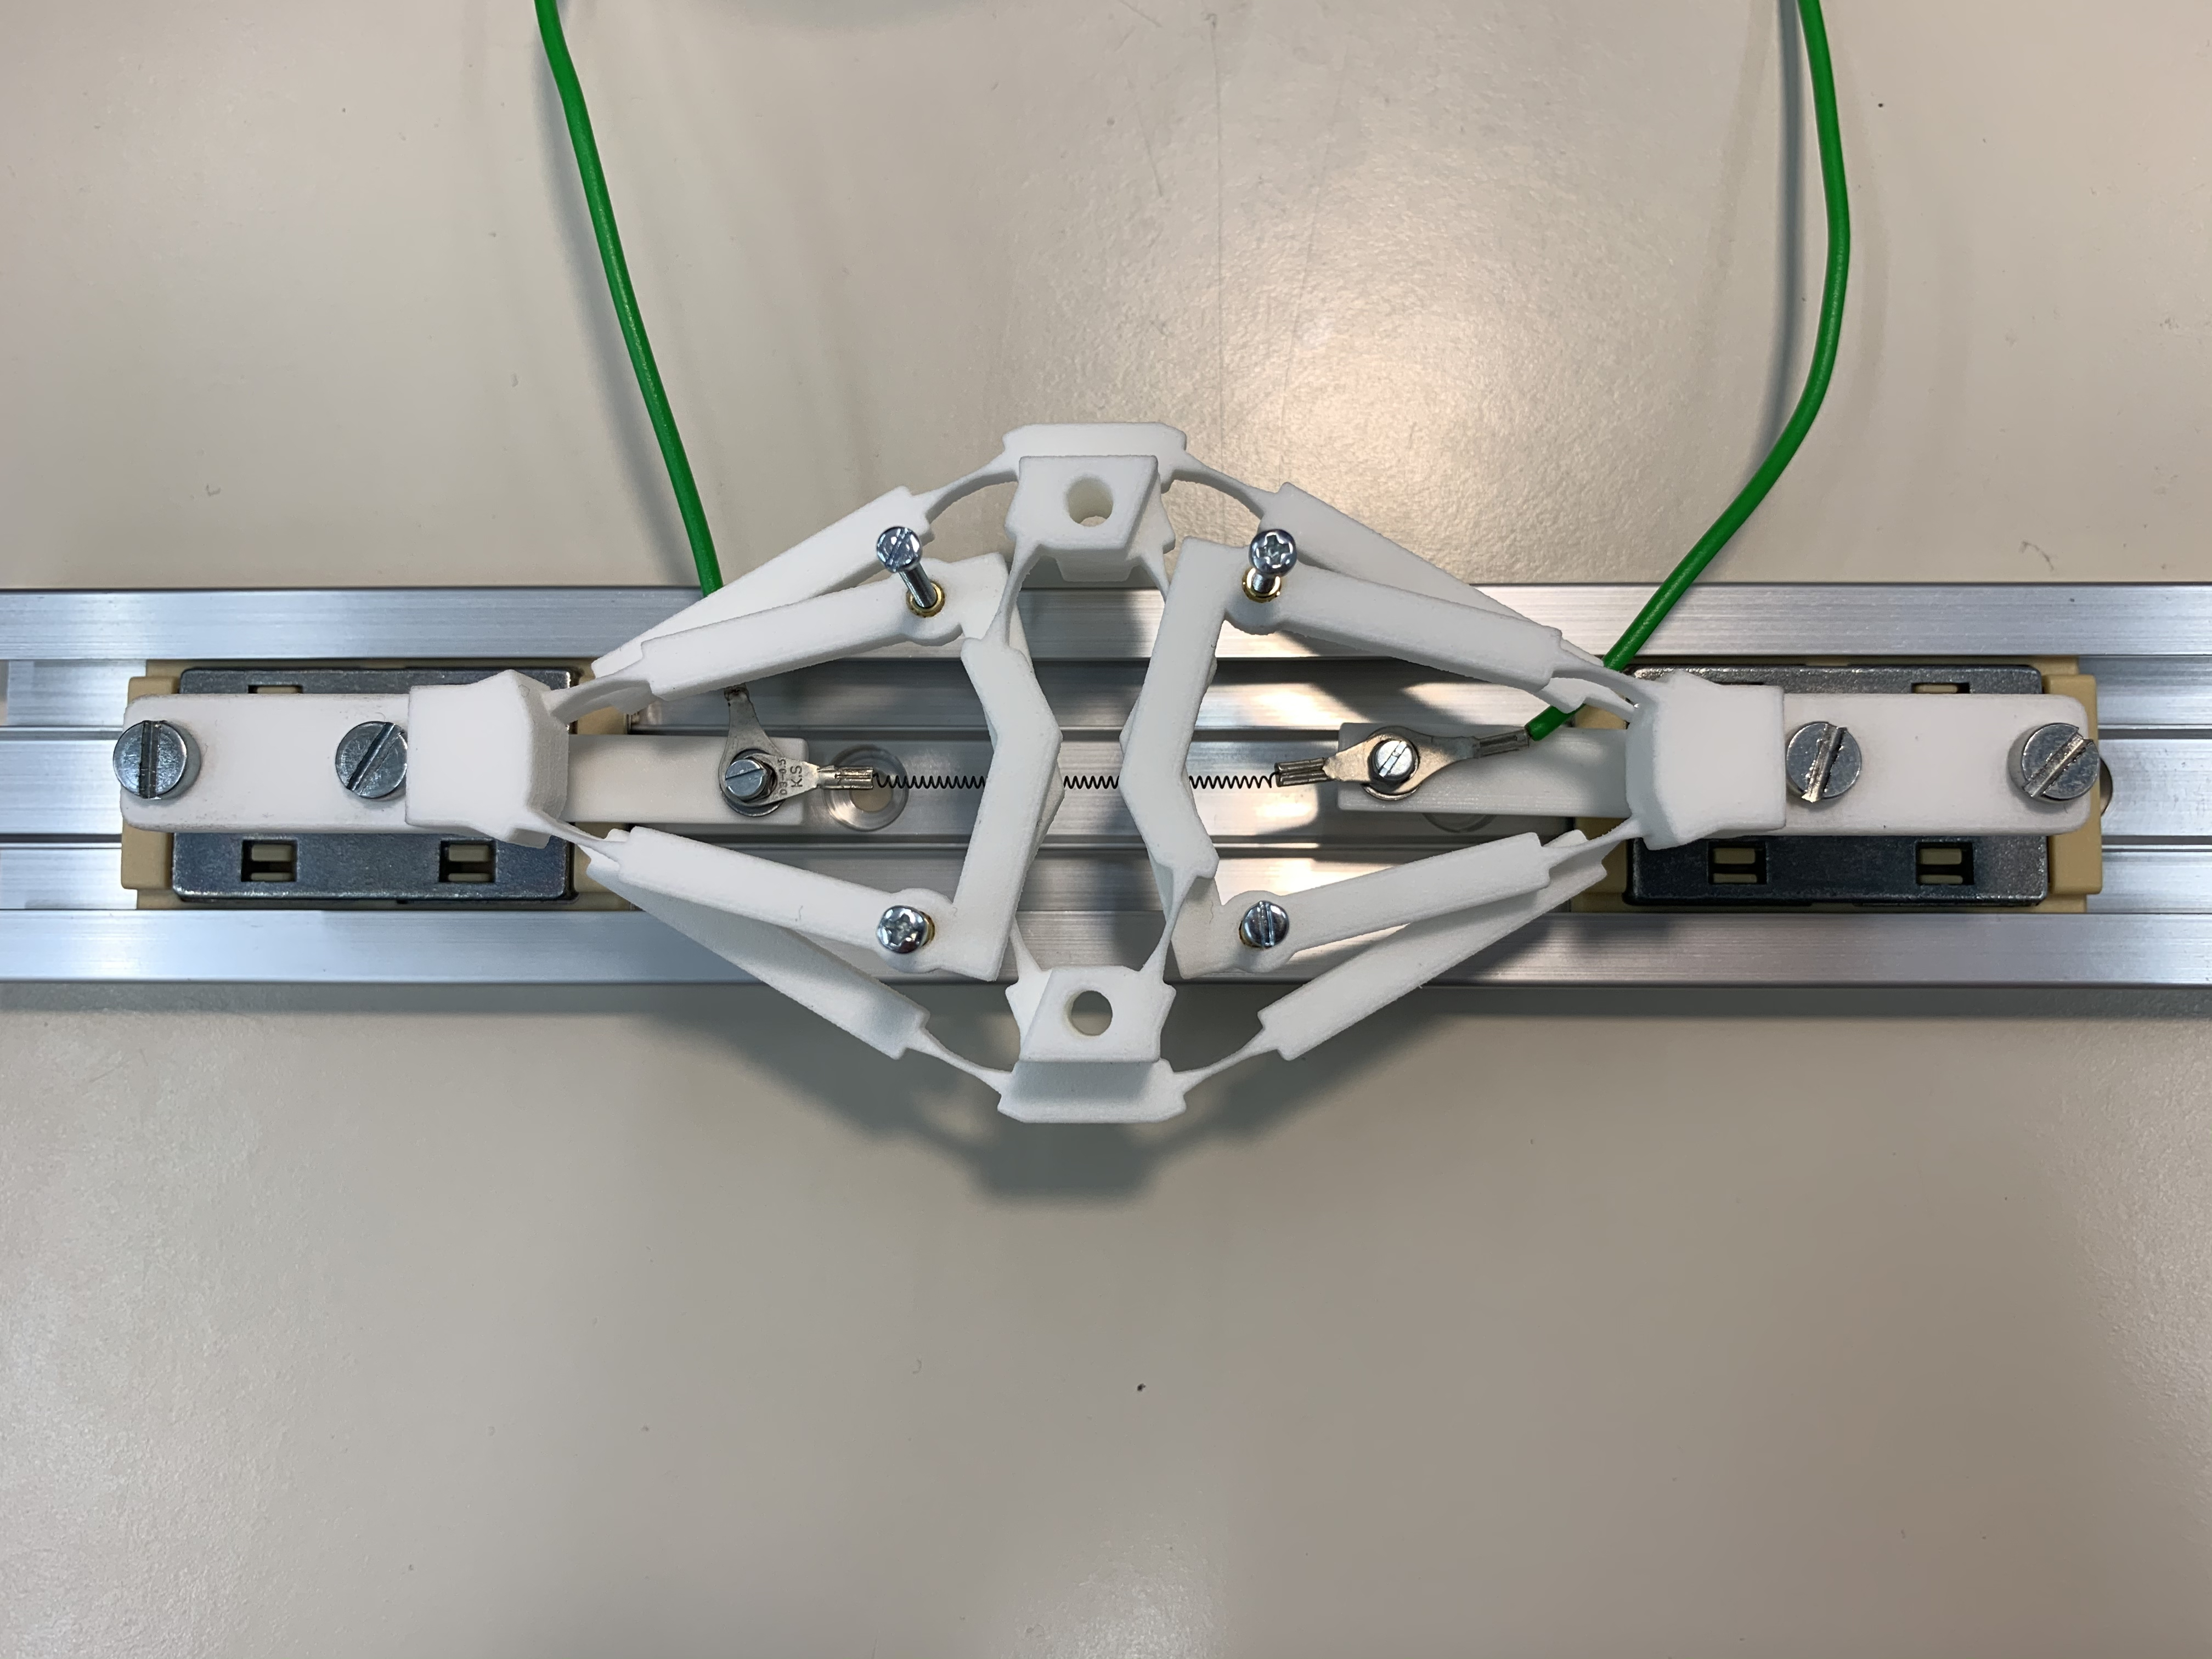
\includegraphics[trim={45cm 50cm 48cm 45cm},clip,width=0.6\columnwidth]{images/chap7/proto_open.jpeg}}}
    \end{overpic}
    }{197.8}{1}{20}};
    \begin{scope}[x={(graph.south east)},y={(graph.north west)}]
       \node[align=left] at (\xFigLetter,\yFigLetter) {\Large \color{white}(a)};
    \end{scope}

     \node[anchor=south west,inner sep=0] (graph1) at (0.06,-3.4){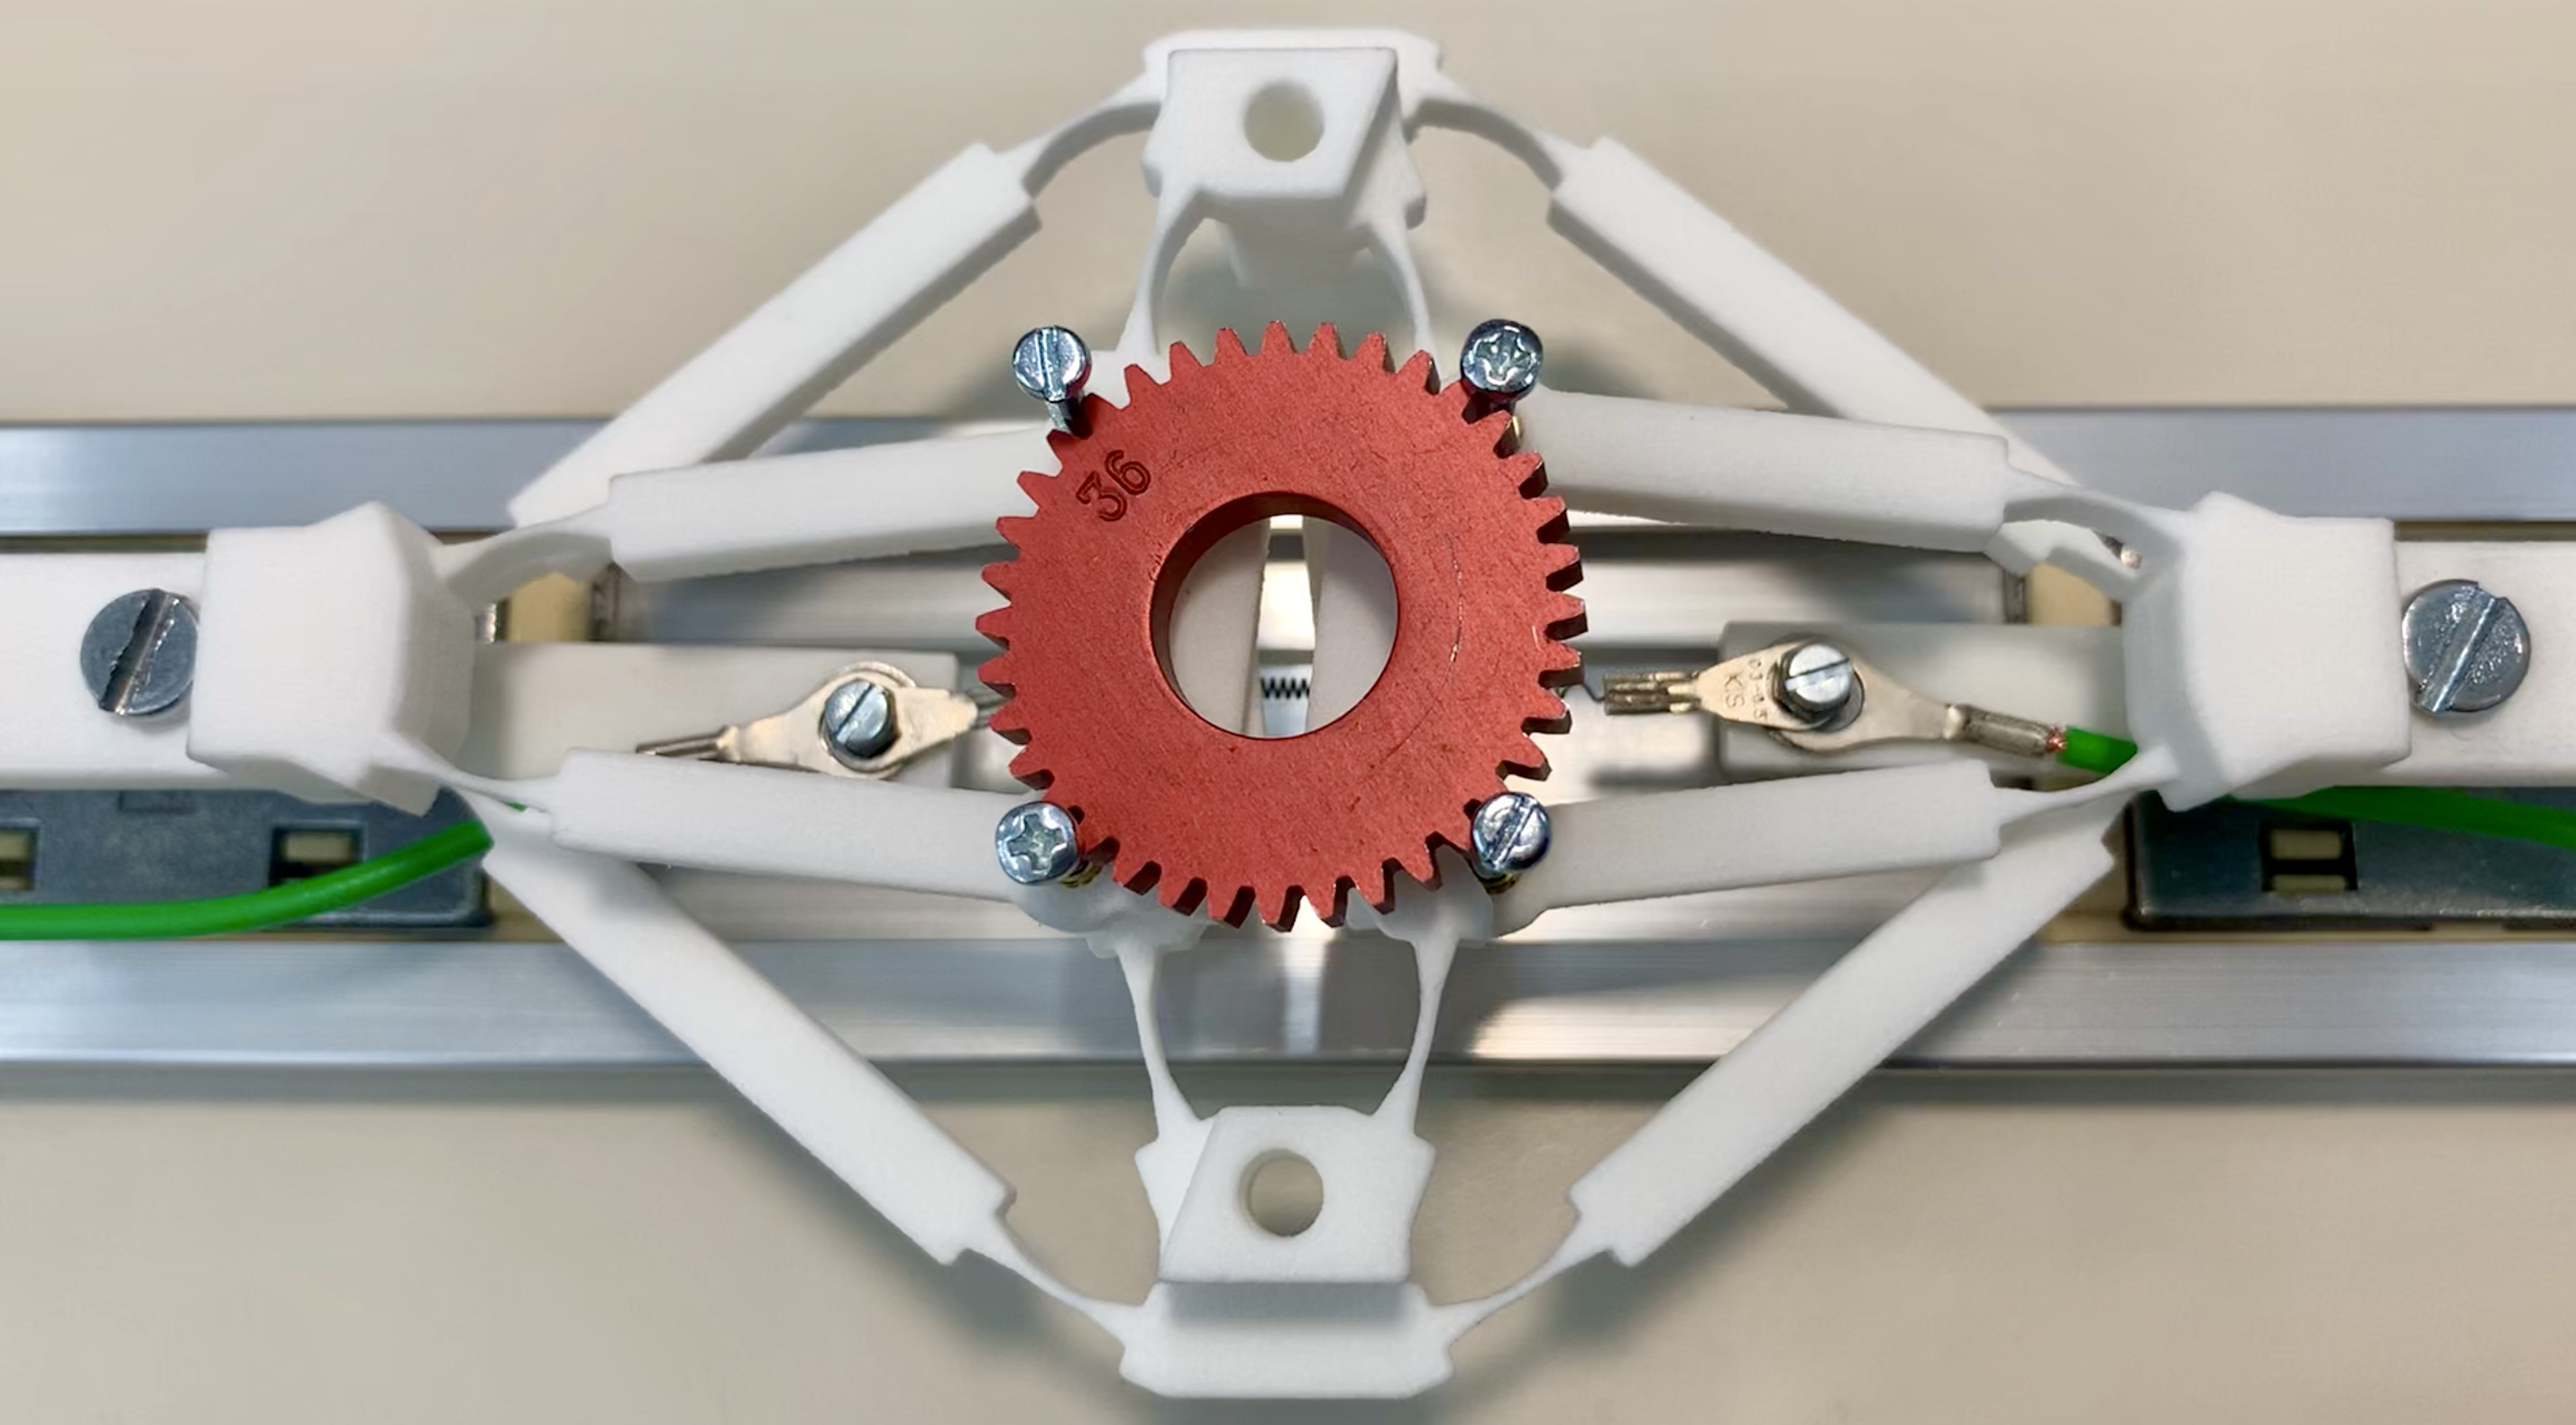
\includegraphics[width=0.98\columnwidth]{images/chap7/closed_with_object.jpeg}};
     \begin{scope}[x={(graph1.south east)},y={(graph1.north west)}]
        \node[align=left] at (\xFigLetter,\yFigLetter) {\Large \color{white}(b)};
     \end{scope}


% \draw[thick,cyan,arrows={-Triangle[angle=90:10pt,cyan,fill=cyan]}] (1.7,\yTopPicture+2.8) -- (3.1,\yTopPicture+2.8);
% \draw[help lines] (0,0) grid (8,4); % $$$$$$$$$$$$$ HELPS A LOT FOR COORDINATES $$$$$$$
 \end{tikzpicture}
\end{document}
}
    \caption{The working prototype of the biased-compliant SMA gripper (a) opened configuration with a $0.2$mm wire diameter SMA coil (framed in red), (b) closed configuration grasping an object.}
    \label{fig:mandrel-finalproto}
\end{figure}

In \cref{fig:mandrel-stroke-estimation}, the validated analytical models are plotted against the force-displacement curves of the SMA coil. This SMA model was estimated using experimental setup where the SMA coil was maintained at a constant temperature using a PID control and a thermal camera, and was then experimentally tested using the pull-tester. With the experimental data, a simplified linear model of the cold and hot SMAs were determined using linear regression. Using these analytical models and the sizing methodology detailed in \cref{subsec:passive-biasing-compliant-mech}, the stroke of the final mandrel gripper can be estimated. In this prototype, the design parameters used are $e=0.5$ mm, $r=15$ mm, $b=4$ mm, $L_h=42.4$ mm, $x_\text{off}=27.5$ mm and $\theta_0 = \frac{\pi}{8}$. Here, an estimated linear output stroke of up to $4.5$ mm is observed for each claw.

\begin{figure}[hbt!] % t for top of the page, H could be put to impose the position of the float
  \centering
  \resizebox{0.7\textwidth}{!}{%% Creator: Matplotlib, PGF backend
%%
%% To include the figure in your LaTeX document, write
%%   \input{<filename>.pgf}
%%
%% Make sure the required packages are loaded in your preamble
%%   \usepackage{pgf}
%%
%% and, on pdftex
%%   \usepackage[utf8]{inputenc}\DeclareUnicodeCharacter{2212}{-}
%%
%% or, on luatex and xetex
%%   \usepackage{unicode-math}
%%
%% Figures using additional raster images can only be included by \input if
%% they are in the same directory as the main LaTeX file. For loading figures
%% from other directories you can use the `import` package
%%   \usepackage{import}
%%
%% and then include the figures with
%%   \import{<path to file>}{<filename>.pgf}
%%
%% Matplotlib used the following preamble
%%
\begingroup%
\makeatletter%
\begin{pgfpicture}%
\pgfpathrectangle{\pgfpointorigin}{\pgfqpoint{6.300000in}{4.700000in}}%
\pgfusepath{use as bounding box, clip}%
\begin{pgfscope}%
\pgfsetbuttcap%
\pgfsetmiterjoin%
\pgfsetlinewidth{0.000000pt}%
\definecolor{currentstroke}{rgb}{0.000000,0.000000,0.000000}%
\pgfsetstrokecolor{currentstroke}%
\pgfsetstrokeopacity{0.000000}%
\pgfsetdash{}{0pt}%
\pgfpathmoveto{\pgfqpoint{-0.000000in}{-0.000000in}}%
\pgfpathlineto{\pgfqpoint{6.300000in}{-0.000000in}}%
\pgfpathlineto{\pgfqpoint{6.300000in}{4.700000in}}%
\pgfpathlineto{\pgfqpoint{-0.000000in}{4.700000in}}%
\pgfpathclose%
\pgfusepath{}%
\end{pgfscope}%
\begin{pgfscope}%
\pgfsetbuttcap%
\pgfsetmiterjoin%
\pgfsetlinewidth{0.000000pt}%
\definecolor{currentstroke}{rgb}{0.000000,0.000000,0.000000}%
\pgfsetstrokecolor{currentstroke}%
\pgfsetstrokeopacity{0.000000}%
\pgfsetdash{}{0pt}%
\pgfpathmoveto{\pgfqpoint{0.590276in}{0.670138in}}%
\pgfpathlineto{\pgfqpoint{6.102085in}{0.670138in}}%
\pgfpathlineto{\pgfqpoint{6.102085in}{4.530556in}}%
\pgfpathlineto{\pgfqpoint{0.590276in}{4.530556in}}%
\pgfpathclose%
\pgfusepath{}%
\end{pgfscope}%
\begin{pgfscope}%
\pgfpathrectangle{\pgfqpoint{0.590276in}{0.670138in}}{\pgfqpoint{5.511808in}{3.860418in}}%
\pgfusepath{clip}%
\pgfsetrectcap%
\pgfsetroundjoin%
\pgfsetlinewidth{0.803000pt}%
\definecolor{currentstroke}{rgb}{0.690196,0.690196,0.690196}%
\pgfsetstrokecolor{currentstroke}%
\pgfsetstrokeopacity{0.200000}%
\pgfsetdash{}{0pt}%
\pgfpathmoveto{\pgfqpoint{0.590276in}{0.670138in}}%
\pgfpathlineto{\pgfqpoint{0.590276in}{4.530556in}}%
\pgfusepath{stroke}%
\end{pgfscope}%
\begin{pgfscope}%
\pgfsetbuttcap%
\pgfsetroundjoin%
\definecolor{currentfill}{rgb}{0.000000,0.000000,0.000000}%
\pgfsetfillcolor{currentfill}%
\pgfsetlinewidth{0.803000pt}%
\definecolor{currentstroke}{rgb}{0.000000,0.000000,0.000000}%
\pgfsetstrokecolor{currentstroke}%
\pgfsetdash{}{0pt}%
\pgfsys@defobject{currentmarker}{\pgfqpoint{0.000000in}{-0.048611in}}{\pgfqpoint{0.000000in}{0.000000in}}{%
\pgfpathmoveto{\pgfqpoint{0.000000in}{0.000000in}}%
\pgfpathlineto{\pgfqpoint{0.000000in}{-0.048611in}}%
\pgfusepath{stroke,fill}%
}%
\begin{pgfscope}%
\pgfsys@transformshift{0.590276in}{0.670138in}%
\pgfsys@useobject{currentmarker}{}%
\end{pgfscope}%
\end{pgfscope}%
\begin{pgfscope}%
\definecolor{textcolor}{rgb}{0.000000,0.000000,0.000000}%
\pgfsetstrokecolor{textcolor}%
\pgfsetfillcolor{textcolor}%
\pgftext[x=0.590276in,y=0.572916in,,top]{\color{textcolor}\rmfamily\fontsize{14.000000}{16.800000}\selectfont \(\displaystyle {0}\)}%
\end{pgfscope}%
\begin{pgfscope}%
\pgfpathrectangle{\pgfqpoint{0.590276in}{0.670138in}}{\pgfqpoint{5.511808in}{3.860418in}}%
\pgfusepath{clip}%
\pgfsetrectcap%
\pgfsetroundjoin%
\pgfsetlinewidth{0.803000pt}%
\definecolor{currentstroke}{rgb}{0.690196,0.690196,0.690196}%
\pgfsetstrokecolor{currentstroke}%
\pgfsetstrokeopacity{0.200000}%
\pgfsetdash{}{0pt}%
\pgfpathmoveto{\pgfqpoint{1.692638in}{0.670138in}}%
\pgfpathlineto{\pgfqpoint{1.692638in}{4.530556in}}%
\pgfusepath{stroke}%
\end{pgfscope}%
\begin{pgfscope}%
\pgfsetbuttcap%
\pgfsetroundjoin%
\definecolor{currentfill}{rgb}{0.000000,0.000000,0.000000}%
\pgfsetfillcolor{currentfill}%
\pgfsetlinewidth{0.803000pt}%
\definecolor{currentstroke}{rgb}{0.000000,0.000000,0.000000}%
\pgfsetstrokecolor{currentstroke}%
\pgfsetdash{}{0pt}%
\pgfsys@defobject{currentmarker}{\pgfqpoint{0.000000in}{-0.048611in}}{\pgfqpoint{0.000000in}{0.000000in}}{%
\pgfpathmoveto{\pgfqpoint{0.000000in}{0.000000in}}%
\pgfpathlineto{\pgfqpoint{0.000000in}{-0.048611in}}%
\pgfusepath{stroke,fill}%
}%
\begin{pgfscope}%
\pgfsys@transformshift{1.692638in}{0.670138in}%
\pgfsys@useobject{currentmarker}{}%
\end{pgfscope}%
\end{pgfscope}%
\begin{pgfscope}%
\definecolor{textcolor}{rgb}{0.000000,0.000000,0.000000}%
\pgfsetstrokecolor{textcolor}%
\pgfsetfillcolor{textcolor}%
\pgftext[x=1.692638in,y=0.572916in,,top]{\color{textcolor}\rmfamily\fontsize{14.000000}{16.800000}\selectfont \(\displaystyle {2}\)}%
\end{pgfscope}%
\begin{pgfscope}%
\pgfpathrectangle{\pgfqpoint{0.590276in}{0.670138in}}{\pgfqpoint{5.511808in}{3.860418in}}%
\pgfusepath{clip}%
\pgfsetrectcap%
\pgfsetroundjoin%
\pgfsetlinewidth{0.803000pt}%
\definecolor{currentstroke}{rgb}{0.690196,0.690196,0.690196}%
\pgfsetstrokecolor{currentstroke}%
\pgfsetstrokeopacity{0.200000}%
\pgfsetdash{}{0pt}%
\pgfpathmoveto{\pgfqpoint{2.794999in}{0.670138in}}%
\pgfpathlineto{\pgfqpoint{2.794999in}{4.530556in}}%
\pgfusepath{stroke}%
\end{pgfscope}%
\begin{pgfscope}%
\pgfsetbuttcap%
\pgfsetroundjoin%
\definecolor{currentfill}{rgb}{0.000000,0.000000,0.000000}%
\pgfsetfillcolor{currentfill}%
\pgfsetlinewidth{0.803000pt}%
\definecolor{currentstroke}{rgb}{0.000000,0.000000,0.000000}%
\pgfsetstrokecolor{currentstroke}%
\pgfsetdash{}{0pt}%
\pgfsys@defobject{currentmarker}{\pgfqpoint{0.000000in}{-0.048611in}}{\pgfqpoint{0.000000in}{0.000000in}}{%
\pgfpathmoveto{\pgfqpoint{0.000000in}{0.000000in}}%
\pgfpathlineto{\pgfqpoint{0.000000in}{-0.048611in}}%
\pgfusepath{stroke,fill}%
}%
\begin{pgfscope}%
\pgfsys@transformshift{2.794999in}{0.670138in}%
\pgfsys@useobject{currentmarker}{}%
\end{pgfscope}%
\end{pgfscope}%
\begin{pgfscope}%
\definecolor{textcolor}{rgb}{0.000000,0.000000,0.000000}%
\pgfsetstrokecolor{textcolor}%
\pgfsetfillcolor{textcolor}%
\pgftext[x=2.794999in,y=0.572916in,,top]{\color{textcolor}\rmfamily\fontsize{14.000000}{16.800000}\selectfont \(\displaystyle {4}\)}%
\end{pgfscope}%
\begin{pgfscope}%
\pgfpathrectangle{\pgfqpoint{0.590276in}{0.670138in}}{\pgfqpoint{5.511808in}{3.860418in}}%
\pgfusepath{clip}%
\pgfsetrectcap%
\pgfsetroundjoin%
\pgfsetlinewidth{0.803000pt}%
\definecolor{currentstroke}{rgb}{0.690196,0.690196,0.690196}%
\pgfsetstrokecolor{currentstroke}%
\pgfsetstrokeopacity{0.200000}%
\pgfsetdash{}{0pt}%
\pgfpathmoveto{\pgfqpoint{3.897361in}{0.670138in}}%
\pgfpathlineto{\pgfqpoint{3.897361in}{4.530556in}}%
\pgfusepath{stroke}%
\end{pgfscope}%
\begin{pgfscope}%
\pgfsetbuttcap%
\pgfsetroundjoin%
\definecolor{currentfill}{rgb}{0.000000,0.000000,0.000000}%
\pgfsetfillcolor{currentfill}%
\pgfsetlinewidth{0.803000pt}%
\definecolor{currentstroke}{rgb}{0.000000,0.000000,0.000000}%
\pgfsetstrokecolor{currentstroke}%
\pgfsetdash{}{0pt}%
\pgfsys@defobject{currentmarker}{\pgfqpoint{0.000000in}{-0.048611in}}{\pgfqpoint{0.000000in}{0.000000in}}{%
\pgfpathmoveto{\pgfqpoint{0.000000in}{0.000000in}}%
\pgfpathlineto{\pgfqpoint{0.000000in}{-0.048611in}}%
\pgfusepath{stroke,fill}%
}%
\begin{pgfscope}%
\pgfsys@transformshift{3.897361in}{0.670138in}%
\pgfsys@useobject{currentmarker}{}%
\end{pgfscope}%
\end{pgfscope}%
\begin{pgfscope}%
\definecolor{textcolor}{rgb}{0.000000,0.000000,0.000000}%
\pgfsetstrokecolor{textcolor}%
\pgfsetfillcolor{textcolor}%
\pgftext[x=3.897361in,y=0.572916in,,top]{\color{textcolor}\rmfamily\fontsize{14.000000}{16.800000}\selectfont \(\displaystyle {6}\)}%
\end{pgfscope}%
\begin{pgfscope}%
\pgfpathrectangle{\pgfqpoint{0.590276in}{0.670138in}}{\pgfqpoint{5.511808in}{3.860418in}}%
\pgfusepath{clip}%
\pgfsetrectcap%
\pgfsetroundjoin%
\pgfsetlinewidth{0.803000pt}%
\definecolor{currentstroke}{rgb}{0.690196,0.690196,0.690196}%
\pgfsetstrokecolor{currentstroke}%
\pgfsetstrokeopacity{0.200000}%
\pgfsetdash{}{0pt}%
\pgfpathmoveto{\pgfqpoint{4.999723in}{0.670138in}}%
\pgfpathlineto{\pgfqpoint{4.999723in}{4.530556in}}%
\pgfusepath{stroke}%
\end{pgfscope}%
\begin{pgfscope}%
\pgfsetbuttcap%
\pgfsetroundjoin%
\definecolor{currentfill}{rgb}{0.000000,0.000000,0.000000}%
\pgfsetfillcolor{currentfill}%
\pgfsetlinewidth{0.803000pt}%
\definecolor{currentstroke}{rgb}{0.000000,0.000000,0.000000}%
\pgfsetstrokecolor{currentstroke}%
\pgfsetdash{}{0pt}%
\pgfsys@defobject{currentmarker}{\pgfqpoint{0.000000in}{-0.048611in}}{\pgfqpoint{0.000000in}{0.000000in}}{%
\pgfpathmoveto{\pgfqpoint{0.000000in}{0.000000in}}%
\pgfpathlineto{\pgfqpoint{0.000000in}{-0.048611in}}%
\pgfusepath{stroke,fill}%
}%
\begin{pgfscope}%
\pgfsys@transformshift{4.999723in}{0.670138in}%
\pgfsys@useobject{currentmarker}{}%
\end{pgfscope}%
\end{pgfscope}%
\begin{pgfscope}%
\definecolor{textcolor}{rgb}{0.000000,0.000000,0.000000}%
\pgfsetstrokecolor{textcolor}%
\pgfsetfillcolor{textcolor}%
\pgftext[x=4.999723in,y=0.572916in,,top]{\color{textcolor}\rmfamily\fontsize{14.000000}{16.800000}\selectfont \(\displaystyle {8}\)}%
\end{pgfscope}%
\begin{pgfscope}%
\pgfpathrectangle{\pgfqpoint{0.590276in}{0.670138in}}{\pgfqpoint{5.511808in}{3.860418in}}%
\pgfusepath{clip}%
\pgfsetrectcap%
\pgfsetroundjoin%
\pgfsetlinewidth{0.803000pt}%
\definecolor{currentstroke}{rgb}{0.690196,0.690196,0.690196}%
\pgfsetstrokecolor{currentstroke}%
\pgfsetstrokeopacity{0.200000}%
\pgfsetdash{}{0pt}%
\pgfpathmoveto{\pgfqpoint{6.102085in}{0.670138in}}%
\pgfpathlineto{\pgfqpoint{6.102085in}{4.530556in}}%
\pgfusepath{stroke}%
\end{pgfscope}%
\begin{pgfscope}%
\pgfsetbuttcap%
\pgfsetroundjoin%
\definecolor{currentfill}{rgb}{0.000000,0.000000,0.000000}%
\pgfsetfillcolor{currentfill}%
\pgfsetlinewidth{0.803000pt}%
\definecolor{currentstroke}{rgb}{0.000000,0.000000,0.000000}%
\pgfsetstrokecolor{currentstroke}%
\pgfsetdash{}{0pt}%
\pgfsys@defobject{currentmarker}{\pgfqpoint{0.000000in}{-0.048611in}}{\pgfqpoint{0.000000in}{0.000000in}}{%
\pgfpathmoveto{\pgfqpoint{0.000000in}{0.000000in}}%
\pgfpathlineto{\pgfqpoint{0.000000in}{-0.048611in}}%
\pgfusepath{stroke,fill}%
}%
\begin{pgfscope}%
\pgfsys@transformshift{6.102085in}{0.670138in}%
\pgfsys@useobject{currentmarker}{}%
\end{pgfscope}%
\end{pgfscope}%
\begin{pgfscope}%
\definecolor{textcolor}{rgb}{0.000000,0.000000,0.000000}%
\pgfsetstrokecolor{textcolor}%
\pgfsetfillcolor{textcolor}%
\pgftext[x=6.102085in,y=0.572916in,,top]{\color{textcolor}\rmfamily\fontsize{14.000000}{16.800000}\selectfont \(\displaystyle {10}\)}%
\end{pgfscope}%
\begin{pgfscope}%
\definecolor{textcolor}{rgb}{0.000000,0.000000,0.000000}%
\pgfsetstrokecolor{textcolor}%
\pgfsetfillcolor{textcolor}%
\pgftext[x=3.346180in,y=0.339583in,,top]{\color{textcolor}\rmfamily\fontsize{16.000000}{19.200000}\selectfont \textbf{Displacement [mm]}}%
\end{pgfscope}%
\begin{pgfscope}%
\pgfpathrectangle{\pgfqpoint{0.590276in}{0.670138in}}{\pgfqpoint{5.511808in}{3.860418in}}%
\pgfusepath{clip}%
\pgfsetrectcap%
\pgfsetroundjoin%
\pgfsetlinewidth{0.803000pt}%
\definecolor{currentstroke}{rgb}{0.690196,0.690196,0.690196}%
\pgfsetstrokecolor{currentstroke}%
\pgfsetstrokeopacity{0.200000}%
\pgfsetdash{}{0pt}%
\pgfpathmoveto{\pgfqpoint{0.590276in}{0.670138in}}%
\pgfpathlineto{\pgfqpoint{6.102085in}{0.670138in}}%
\pgfusepath{stroke}%
\end{pgfscope}%
\begin{pgfscope}%
\pgfsetbuttcap%
\pgfsetroundjoin%
\definecolor{currentfill}{rgb}{0.000000,0.000000,0.000000}%
\pgfsetfillcolor{currentfill}%
\pgfsetlinewidth{0.803000pt}%
\definecolor{currentstroke}{rgb}{0.000000,0.000000,0.000000}%
\pgfsetstrokecolor{currentstroke}%
\pgfsetdash{}{0pt}%
\pgfsys@defobject{currentmarker}{\pgfqpoint{-0.048611in}{0.000000in}}{\pgfqpoint{-0.000000in}{0.000000in}}{%
\pgfpathmoveto{\pgfqpoint{-0.000000in}{0.000000in}}%
\pgfpathlineto{\pgfqpoint{-0.048611in}{0.000000in}}%
\pgfusepath{stroke,fill}%
}%
\begin{pgfscope}%
\pgfsys@transformshift{0.590276in}{0.670138in}%
\pgfsys@useobject{currentmarker}{}%
\end{pgfscope}%
\end{pgfscope}%
\begin{pgfscope}%
\definecolor{textcolor}{rgb}{0.000000,0.000000,0.000000}%
\pgfsetstrokecolor{textcolor}%
\pgfsetfillcolor{textcolor}%
\pgftext[x=0.395138in, y=0.600694in, left, base]{\color{textcolor}\rmfamily\fontsize{14.000000}{16.800000}\selectfont \(\displaystyle {0}\)}%
\end{pgfscope}%
\begin{pgfscope}%
\pgfpathrectangle{\pgfqpoint{0.590276in}{0.670138in}}{\pgfqpoint{5.511808in}{3.860418in}}%
\pgfusepath{clip}%
\pgfsetrectcap%
\pgfsetroundjoin%
\pgfsetlinewidth{0.803000pt}%
\definecolor{currentstroke}{rgb}{0.690196,0.690196,0.690196}%
\pgfsetstrokecolor{currentstroke}%
\pgfsetstrokeopacity{0.200000}%
\pgfsetdash{}{0pt}%
\pgfpathmoveto{\pgfqpoint{0.590276in}{1.313541in}}%
\pgfpathlineto{\pgfqpoint{6.102085in}{1.313541in}}%
\pgfusepath{stroke}%
\end{pgfscope}%
\begin{pgfscope}%
\pgfsetbuttcap%
\pgfsetroundjoin%
\definecolor{currentfill}{rgb}{0.000000,0.000000,0.000000}%
\pgfsetfillcolor{currentfill}%
\pgfsetlinewidth{0.803000pt}%
\definecolor{currentstroke}{rgb}{0.000000,0.000000,0.000000}%
\pgfsetstrokecolor{currentstroke}%
\pgfsetdash{}{0pt}%
\pgfsys@defobject{currentmarker}{\pgfqpoint{-0.048611in}{0.000000in}}{\pgfqpoint{-0.000000in}{0.000000in}}{%
\pgfpathmoveto{\pgfqpoint{-0.000000in}{0.000000in}}%
\pgfpathlineto{\pgfqpoint{-0.048611in}{0.000000in}}%
\pgfusepath{stroke,fill}%
}%
\begin{pgfscope}%
\pgfsys@transformshift{0.590276in}{1.313541in}%
\pgfsys@useobject{currentmarker}{}%
\end{pgfscope}%
\end{pgfscope}%
\begin{pgfscope}%
\definecolor{textcolor}{rgb}{0.000000,0.000000,0.000000}%
\pgfsetstrokecolor{textcolor}%
\pgfsetfillcolor{textcolor}%
\pgftext[x=0.395138in, y=1.244097in, left, base]{\color{textcolor}\rmfamily\fontsize{14.000000}{16.800000}\selectfont \(\displaystyle {1}\)}%
\end{pgfscope}%
\begin{pgfscope}%
\pgfpathrectangle{\pgfqpoint{0.590276in}{0.670138in}}{\pgfqpoint{5.511808in}{3.860418in}}%
\pgfusepath{clip}%
\pgfsetrectcap%
\pgfsetroundjoin%
\pgfsetlinewidth{0.803000pt}%
\definecolor{currentstroke}{rgb}{0.690196,0.690196,0.690196}%
\pgfsetstrokecolor{currentstroke}%
\pgfsetstrokeopacity{0.200000}%
\pgfsetdash{}{0pt}%
\pgfpathmoveto{\pgfqpoint{0.590276in}{1.956944in}}%
\pgfpathlineto{\pgfqpoint{6.102085in}{1.956944in}}%
\pgfusepath{stroke}%
\end{pgfscope}%
\begin{pgfscope}%
\pgfsetbuttcap%
\pgfsetroundjoin%
\definecolor{currentfill}{rgb}{0.000000,0.000000,0.000000}%
\pgfsetfillcolor{currentfill}%
\pgfsetlinewidth{0.803000pt}%
\definecolor{currentstroke}{rgb}{0.000000,0.000000,0.000000}%
\pgfsetstrokecolor{currentstroke}%
\pgfsetdash{}{0pt}%
\pgfsys@defobject{currentmarker}{\pgfqpoint{-0.048611in}{0.000000in}}{\pgfqpoint{-0.000000in}{0.000000in}}{%
\pgfpathmoveto{\pgfqpoint{-0.000000in}{0.000000in}}%
\pgfpathlineto{\pgfqpoint{-0.048611in}{0.000000in}}%
\pgfusepath{stroke,fill}%
}%
\begin{pgfscope}%
\pgfsys@transformshift{0.590276in}{1.956944in}%
\pgfsys@useobject{currentmarker}{}%
\end{pgfscope}%
\end{pgfscope}%
\begin{pgfscope}%
\definecolor{textcolor}{rgb}{0.000000,0.000000,0.000000}%
\pgfsetstrokecolor{textcolor}%
\pgfsetfillcolor{textcolor}%
\pgftext[x=0.395138in, y=1.887500in, left, base]{\color{textcolor}\rmfamily\fontsize{14.000000}{16.800000}\selectfont \(\displaystyle {2}\)}%
\end{pgfscope}%
\begin{pgfscope}%
\pgfpathrectangle{\pgfqpoint{0.590276in}{0.670138in}}{\pgfqpoint{5.511808in}{3.860418in}}%
\pgfusepath{clip}%
\pgfsetrectcap%
\pgfsetroundjoin%
\pgfsetlinewidth{0.803000pt}%
\definecolor{currentstroke}{rgb}{0.690196,0.690196,0.690196}%
\pgfsetstrokecolor{currentstroke}%
\pgfsetstrokeopacity{0.200000}%
\pgfsetdash{}{0pt}%
\pgfpathmoveto{\pgfqpoint{0.590276in}{2.600347in}}%
\pgfpathlineto{\pgfqpoint{6.102085in}{2.600347in}}%
\pgfusepath{stroke}%
\end{pgfscope}%
\begin{pgfscope}%
\pgfsetbuttcap%
\pgfsetroundjoin%
\definecolor{currentfill}{rgb}{0.000000,0.000000,0.000000}%
\pgfsetfillcolor{currentfill}%
\pgfsetlinewidth{0.803000pt}%
\definecolor{currentstroke}{rgb}{0.000000,0.000000,0.000000}%
\pgfsetstrokecolor{currentstroke}%
\pgfsetdash{}{0pt}%
\pgfsys@defobject{currentmarker}{\pgfqpoint{-0.048611in}{0.000000in}}{\pgfqpoint{-0.000000in}{0.000000in}}{%
\pgfpathmoveto{\pgfqpoint{-0.000000in}{0.000000in}}%
\pgfpathlineto{\pgfqpoint{-0.048611in}{0.000000in}}%
\pgfusepath{stroke,fill}%
}%
\begin{pgfscope}%
\pgfsys@transformshift{0.590276in}{2.600347in}%
\pgfsys@useobject{currentmarker}{}%
\end{pgfscope}%
\end{pgfscope}%
\begin{pgfscope}%
\definecolor{textcolor}{rgb}{0.000000,0.000000,0.000000}%
\pgfsetstrokecolor{textcolor}%
\pgfsetfillcolor{textcolor}%
\pgftext[x=0.395138in, y=2.530903in, left, base]{\color{textcolor}\rmfamily\fontsize{14.000000}{16.800000}\selectfont \(\displaystyle {3}\)}%
\end{pgfscope}%
\begin{pgfscope}%
\pgfpathrectangle{\pgfqpoint{0.590276in}{0.670138in}}{\pgfqpoint{5.511808in}{3.860418in}}%
\pgfusepath{clip}%
\pgfsetrectcap%
\pgfsetroundjoin%
\pgfsetlinewidth{0.803000pt}%
\definecolor{currentstroke}{rgb}{0.690196,0.690196,0.690196}%
\pgfsetstrokecolor{currentstroke}%
\pgfsetstrokeopacity{0.200000}%
\pgfsetdash{}{0pt}%
\pgfpathmoveto{\pgfqpoint{0.590276in}{3.243750in}}%
\pgfpathlineto{\pgfqpoint{6.102085in}{3.243750in}}%
\pgfusepath{stroke}%
\end{pgfscope}%
\begin{pgfscope}%
\pgfsetbuttcap%
\pgfsetroundjoin%
\definecolor{currentfill}{rgb}{0.000000,0.000000,0.000000}%
\pgfsetfillcolor{currentfill}%
\pgfsetlinewidth{0.803000pt}%
\definecolor{currentstroke}{rgb}{0.000000,0.000000,0.000000}%
\pgfsetstrokecolor{currentstroke}%
\pgfsetdash{}{0pt}%
\pgfsys@defobject{currentmarker}{\pgfqpoint{-0.048611in}{0.000000in}}{\pgfqpoint{-0.000000in}{0.000000in}}{%
\pgfpathmoveto{\pgfqpoint{-0.000000in}{0.000000in}}%
\pgfpathlineto{\pgfqpoint{-0.048611in}{0.000000in}}%
\pgfusepath{stroke,fill}%
}%
\begin{pgfscope}%
\pgfsys@transformshift{0.590276in}{3.243750in}%
\pgfsys@useobject{currentmarker}{}%
\end{pgfscope}%
\end{pgfscope}%
\begin{pgfscope}%
\definecolor{textcolor}{rgb}{0.000000,0.000000,0.000000}%
\pgfsetstrokecolor{textcolor}%
\pgfsetfillcolor{textcolor}%
\pgftext[x=0.395138in, y=3.174306in, left, base]{\color{textcolor}\rmfamily\fontsize{14.000000}{16.800000}\selectfont \(\displaystyle {4}\)}%
\end{pgfscope}%
\begin{pgfscope}%
\pgfpathrectangle{\pgfqpoint{0.590276in}{0.670138in}}{\pgfqpoint{5.511808in}{3.860418in}}%
\pgfusepath{clip}%
\pgfsetrectcap%
\pgfsetroundjoin%
\pgfsetlinewidth{0.803000pt}%
\definecolor{currentstroke}{rgb}{0.690196,0.690196,0.690196}%
\pgfsetstrokecolor{currentstroke}%
\pgfsetstrokeopacity{0.200000}%
\pgfsetdash{}{0pt}%
\pgfpathmoveto{\pgfqpoint{0.590276in}{3.887153in}}%
\pgfpathlineto{\pgfqpoint{6.102085in}{3.887153in}}%
\pgfusepath{stroke}%
\end{pgfscope}%
\begin{pgfscope}%
\pgfsetbuttcap%
\pgfsetroundjoin%
\definecolor{currentfill}{rgb}{0.000000,0.000000,0.000000}%
\pgfsetfillcolor{currentfill}%
\pgfsetlinewidth{0.803000pt}%
\definecolor{currentstroke}{rgb}{0.000000,0.000000,0.000000}%
\pgfsetstrokecolor{currentstroke}%
\pgfsetdash{}{0pt}%
\pgfsys@defobject{currentmarker}{\pgfqpoint{-0.048611in}{0.000000in}}{\pgfqpoint{-0.000000in}{0.000000in}}{%
\pgfpathmoveto{\pgfqpoint{-0.000000in}{0.000000in}}%
\pgfpathlineto{\pgfqpoint{-0.048611in}{0.000000in}}%
\pgfusepath{stroke,fill}%
}%
\begin{pgfscope}%
\pgfsys@transformshift{0.590276in}{3.887153in}%
\pgfsys@useobject{currentmarker}{}%
\end{pgfscope}%
\end{pgfscope}%
\begin{pgfscope}%
\definecolor{textcolor}{rgb}{0.000000,0.000000,0.000000}%
\pgfsetstrokecolor{textcolor}%
\pgfsetfillcolor{textcolor}%
\pgftext[x=0.395138in, y=3.817708in, left, base]{\color{textcolor}\rmfamily\fontsize{14.000000}{16.800000}\selectfont \(\displaystyle {5}\)}%
\end{pgfscope}%
\begin{pgfscope}%
\pgfpathrectangle{\pgfqpoint{0.590276in}{0.670138in}}{\pgfqpoint{5.511808in}{3.860418in}}%
\pgfusepath{clip}%
\pgfsetrectcap%
\pgfsetroundjoin%
\pgfsetlinewidth{0.803000pt}%
\definecolor{currentstroke}{rgb}{0.690196,0.690196,0.690196}%
\pgfsetstrokecolor{currentstroke}%
\pgfsetstrokeopacity{0.200000}%
\pgfsetdash{}{0pt}%
\pgfpathmoveto{\pgfqpoint{0.590276in}{4.530556in}}%
\pgfpathlineto{\pgfqpoint{6.102085in}{4.530556in}}%
\pgfusepath{stroke}%
\end{pgfscope}%
\begin{pgfscope}%
\pgfsetbuttcap%
\pgfsetroundjoin%
\definecolor{currentfill}{rgb}{0.000000,0.000000,0.000000}%
\pgfsetfillcolor{currentfill}%
\pgfsetlinewidth{0.803000pt}%
\definecolor{currentstroke}{rgb}{0.000000,0.000000,0.000000}%
\pgfsetstrokecolor{currentstroke}%
\pgfsetdash{}{0pt}%
\pgfsys@defobject{currentmarker}{\pgfqpoint{-0.048611in}{0.000000in}}{\pgfqpoint{-0.000000in}{0.000000in}}{%
\pgfpathmoveto{\pgfqpoint{-0.000000in}{0.000000in}}%
\pgfpathlineto{\pgfqpoint{-0.048611in}{0.000000in}}%
\pgfusepath{stroke,fill}%
}%
\begin{pgfscope}%
\pgfsys@transformshift{0.590276in}{4.530556in}%
\pgfsys@useobject{currentmarker}{}%
\end{pgfscope}%
\end{pgfscope}%
\begin{pgfscope}%
\definecolor{textcolor}{rgb}{0.000000,0.000000,0.000000}%
\pgfsetstrokecolor{textcolor}%
\pgfsetfillcolor{textcolor}%
\pgftext[x=0.395138in, y=4.461111in, left, base]{\color{textcolor}\rmfamily\fontsize{14.000000}{16.800000}\selectfont \(\displaystyle {6}\)}%
\end{pgfscope}%
\begin{pgfscope}%
\definecolor{textcolor}{rgb}{0.000000,0.000000,0.000000}%
\pgfsetstrokecolor{textcolor}%
\pgfsetfillcolor{textcolor}%
\pgftext[x=0.339583in,y=2.600347in,,bottom,rotate=90.000000]{\color{textcolor}\rmfamily\fontsize{16.000000}{19.200000}\selectfont \textbf{Force [N]}}%
\end{pgfscope}%
\begin{pgfscope}%
\pgfpathrectangle{\pgfqpoint{0.590276in}{0.670138in}}{\pgfqpoint{5.511808in}{3.860418in}}%
\pgfusepath{clip}%
\pgfsetrectcap%
\pgfsetroundjoin%
\pgfsetlinewidth{1.505625pt}%
\definecolor{currentstroke}{rgb}{0.145098,0.560784,0.105882}%
\pgfsetstrokecolor{currentstroke}%
\pgfsetdash{}{0pt}%
\pgfpathmoveto{\pgfqpoint{0.586943in}{2.450726in}}%
\pgfpathlineto{\pgfqpoint{0.818543in}{2.438361in}}%
\pgfpathlineto{\pgfqpoint{1.172078in}{2.419234in}}%
\pgfpathlineto{\pgfqpoint{1.525613in}{2.399840in}}%
\pgfpathlineto{\pgfqpoint{1.879148in}{2.380160in}}%
\pgfpathlineto{\pgfqpoint{2.232684in}{2.360176in}}%
\pgfpathlineto{\pgfqpoint{2.586219in}{2.339867in}}%
\pgfpathlineto{\pgfqpoint{2.939754in}{2.319213in}}%
\pgfpathlineto{\pgfqpoint{3.293289in}{2.298190in}}%
\pgfpathlineto{\pgfqpoint{3.646824in}{2.276773in}}%
\pgfpathlineto{\pgfqpoint{4.000360in}{2.254936in}}%
\pgfpathlineto{\pgfqpoint{4.353895in}{2.232650in}}%
\pgfpathlineto{\pgfqpoint{4.707430in}{2.209883in}}%
\pgfpathlineto{\pgfqpoint{5.060965in}{2.186601in}}%
\pgfpathlineto{\pgfqpoint{5.414500in}{2.162767in}}%
\pgfpathlineto{\pgfqpoint{5.768036in}{2.138342in}}%
\pgfpathlineto{\pgfqpoint{6.105418in}{2.114426in}}%
\pgfusepath{stroke}%
\end{pgfscope}%
\begin{pgfscope}%
\pgfpathrectangle{\pgfqpoint{0.590276in}{0.670138in}}{\pgfqpoint{5.511808in}{3.860418in}}%
\pgfusepath{clip}%
\pgfsetrectcap%
\pgfsetroundjoin%
\pgfsetlinewidth{1.505625pt}%
\definecolor{currentstroke}{rgb}{0.000000,0.447059,0.741176}%
\pgfsetstrokecolor{currentstroke}%
\pgfsetdash{}{0pt}%
\pgfpathmoveto{\pgfqpoint{0.586943in}{0.739115in}}%
\pgfpathlineto{\pgfqpoint{0.863083in}{0.843539in}}%
\pgfpathlineto{\pgfqpoint{1.216618in}{0.977231in}}%
\pgfpathlineto{\pgfqpoint{1.570153in}{1.110922in}}%
\pgfpathlineto{\pgfqpoint{1.923688in}{1.244614in}}%
\pgfpathlineto{\pgfqpoint{2.277224in}{1.378306in}}%
\pgfpathlineto{\pgfqpoint{2.630759in}{1.511997in}}%
\pgfpathlineto{\pgfqpoint{2.984294in}{1.645689in}}%
\pgfpathlineto{\pgfqpoint{3.337829in}{1.779381in}}%
\pgfpathlineto{\pgfqpoint{3.691364in}{1.913072in}}%
\pgfpathlineto{\pgfqpoint{4.044900in}{2.046764in}}%
\pgfpathlineto{\pgfqpoint{4.398435in}{2.180456in}}%
\pgfpathlineto{\pgfqpoint{4.751970in}{2.314147in}}%
\pgfpathlineto{\pgfqpoint{5.105505in}{2.447839in}}%
\pgfpathlineto{\pgfqpoint{5.459040in}{2.581531in}}%
\pgfpathlineto{\pgfqpoint{5.812575in}{2.715222in}}%
\pgfpathlineto{\pgfqpoint{6.105418in}{2.825963in}}%
\pgfusepath{stroke}%
\end{pgfscope}%
\begin{pgfscope}%
\pgfpathrectangle{\pgfqpoint{0.590276in}{0.670138in}}{\pgfqpoint{5.511808in}{3.860418in}}%
\pgfusepath{clip}%
\pgfsetrectcap%
\pgfsetroundjoin%
\pgfsetlinewidth{1.505625pt}%
\definecolor{currentstroke}{rgb}{0.768627,0.000000,0.047059}%
\pgfsetstrokecolor{currentstroke}%
\pgfsetdash{}{0pt}%
\pgfpathmoveto{\pgfqpoint{0.612703in}{0.666805in}}%
\pgfpathlineto{\pgfqpoint{0.863083in}{0.975248in}}%
\pgfpathlineto{\pgfqpoint{1.216618in}{1.410768in}}%
\pgfpathlineto{\pgfqpoint{1.570153in}{1.846288in}}%
\pgfpathlineto{\pgfqpoint{1.923688in}{2.281809in}}%
\pgfpathlineto{\pgfqpoint{2.277224in}{2.717329in}}%
\pgfpathlineto{\pgfqpoint{2.630759in}{3.152849in}}%
\pgfpathlineto{\pgfqpoint{2.984294in}{3.588370in}}%
\pgfpathlineto{\pgfqpoint{3.337829in}{4.023890in}}%
\pgfpathlineto{\pgfqpoint{3.691364in}{4.459410in}}%
\pgfpathlineto{\pgfqpoint{3.751823in}{4.533889in}}%
\pgfusepath{stroke}%
\end{pgfscope}%
\begin{pgfscope}%
\pgfsetrectcap%
\pgfsetmiterjoin%
\pgfsetlinewidth{0.803000pt}%
\definecolor{currentstroke}{rgb}{0.000000,0.000000,0.000000}%
\pgfsetstrokecolor{currentstroke}%
\pgfsetdash{}{0pt}%
\pgfpathmoveto{\pgfqpoint{0.590276in}{0.670138in}}%
\pgfpathlineto{\pgfqpoint{0.590276in}{4.530556in}}%
\pgfusepath{stroke}%
\end{pgfscope}%
\begin{pgfscope}%
\pgfsetrectcap%
\pgfsetmiterjoin%
\pgfsetlinewidth{0.803000pt}%
\definecolor{currentstroke}{rgb}{0.000000,0.000000,0.000000}%
\pgfsetstrokecolor{currentstroke}%
\pgfsetdash{}{0pt}%
\pgfpathmoveto{\pgfqpoint{6.102085in}{0.670138in}}%
\pgfpathlineto{\pgfqpoint{6.102085in}{4.530556in}}%
\pgfusepath{stroke}%
\end{pgfscope}%
\begin{pgfscope}%
\pgfsetrectcap%
\pgfsetmiterjoin%
\pgfsetlinewidth{0.803000pt}%
\definecolor{currentstroke}{rgb}{0.000000,0.000000,0.000000}%
\pgfsetstrokecolor{currentstroke}%
\pgfsetdash{}{0pt}%
\pgfpathmoveto{\pgfqpoint{0.590276in}{0.670138in}}%
\pgfpathlineto{\pgfqpoint{6.102085in}{0.670138in}}%
\pgfusepath{stroke}%
\end{pgfscope}%
\begin{pgfscope}%
\pgfsetrectcap%
\pgfsetmiterjoin%
\pgfsetlinewidth{0.803000pt}%
\definecolor{currentstroke}{rgb}{0.000000,0.000000,0.000000}%
\pgfsetstrokecolor{currentstroke}%
\pgfsetdash{}{0pt}%
\pgfpathmoveto{\pgfqpoint{0.590276in}{4.530556in}}%
\pgfpathlineto{\pgfqpoint{6.102085in}{4.530556in}}%
\pgfusepath{stroke}%
\end{pgfscope}%
\begin{pgfscope}%
\pgfsetbuttcap%
\pgfsetmiterjoin%
\definecolor{currentfill}{rgb}{1.000000,1.000000,1.000000}%
\pgfsetfillcolor{currentfill}%
\pgfsetfillopacity{0.800000}%
\pgfsetlinewidth{1.003750pt}%
\definecolor{currentstroke}{rgb}{0.800000,0.800000,0.800000}%
\pgfsetstrokecolor{currentstroke}%
\pgfsetstrokeopacity{0.800000}%
\pgfsetdash{}{0pt}%
\pgfpathmoveto{\pgfqpoint{3.640200in}{3.629630in}}%
\pgfpathlineto{\pgfqpoint{5.975696in}{3.629630in}}%
\pgfpathquadraticcurveto{\pgfqpoint{6.011807in}{3.629630in}}{\pgfqpoint{6.011807in}{3.665742in}}%
\pgfpathlineto{\pgfqpoint{6.011807in}{4.404167in}}%
\pgfpathquadraticcurveto{\pgfqpoint{6.011807in}{4.440278in}}{\pgfqpoint{5.975696in}{4.440278in}}%
\pgfpathlineto{\pgfqpoint{3.640200in}{4.440278in}}%
\pgfpathquadraticcurveto{\pgfqpoint{3.604089in}{4.440278in}}{\pgfqpoint{3.604089in}{4.404167in}}%
\pgfpathlineto{\pgfqpoint{3.604089in}{3.665742in}}%
\pgfpathquadraticcurveto{\pgfqpoint{3.604089in}{3.629630in}}{\pgfqpoint{3.640200in}{3.629630in}}%
\pgfpathclose%
\pgfusepath{stroke,fill}%
\end{pgfscope}%
\begin{pgfscope}%
\pgfsetrectcap%
\pgfsetroundjoin%
\pgfsetlinewidth{1.505625pt}%
\definecolor{currentstroke}{rgb}{0.768627,0.000000,0.047059}%
\pgfsetstrokecolor{currentstroke}%
\pgfsetdash{}{0pt}%
\pgfpathmoveto{\pgfqpoint{3.676311in}{4.304861in}}%
\pgfpathlineto{\pgfqpoint{4.037422in}{4.304861in}}%
\pgfusepath{stroke}%
\end{pgfscope}%
\begin{pgfscope}%
\definecolor{textcolor}{rgb}{0.000000,0.000000,0.000000}%
\pgfsetstrokecolor{textcolor}%
\pgfsetfillcolor{textcolor}%
\pgftext[x=4.181867in,y=4.241667in,left,base]{\color{textcolor}\rmfamily\fontsize{13.000000}{15.600000}\selectfont SMA at 120°C}%
\end{pgfscope}%
\begin{pgfscope}%
\pgfsetrectcap%
\pgfsetroundjoin%
\pgfsetlinewidth{1.505625pt}%
\definecolor{currentstroke}{rgb}{0.000000,0.447059,0.741176}%
\pgfsetstrokecolor{currentstroke}%
\pgfsetdash{}{0pt}%
\pgfpathmoveto{\pgfqpoint{3.676311in}{4.055788in}}%
\pgfpathlineto{\pgfqpoint{4.037422in}{4.055788in}}%
\pgfusepath{stroke}%
\end{pgfscope}%
\begin{pgfscope}%
\definecolor{textcolor}{rgb}{0.000000,0.000000,0.000000}%
\pgfsetstrokecolor{textcolor}%
\pgfsetfillcolor{textcolor}%
\pgftext[x=4.181867in,y=3.992593in,left,base]{\color{textcolor}\rmfamily\fontsize{13.000000}{15.600000}\selectfont SMA at 30°C}%
\end{pgfscope}%
\begin{pgfscope}%
\pgfsetrectcap%
\pgfsetroundjoin%
\pgfsetlinewidth{1.505625pt}%
\definecolor{currentstroke}{rgb}{0.145098,0.560784,0.105882}%
\pgfsetstrokecolor{currentstroke}%
\pgfsetdash{}{0pt}%
\pgfpathmoveto{\pgfqpoint{3.676311in}{3.806714in}}%
\pgfpathlineto{\pgfqpoint{4.037422in}{3.806714in}}%
\pgfusepath{stroke}%
\end{pgfscope}%
\begin{pgfscope}%
\definecolor{textcolor}{rgb}{0.000000,0.000000,0.000000}%
\pgfsetstrokecolor{textcolor}%
\pgfsetfillcolor{textcolor}%
\pgftext[x=4.181867in,y=3.743519in,left,base]{\color{textcolor}\rmfamily\fontsize{13.000000}{15.600000}\selectfont Analytical model \(\displaystyle F(\Delta x)\)}%
\end{pgfscope}%
\end{pgfpicture}%
\makeatother%
\endgroup%
}
  \caption{The sizing diagram of the SMA mandrel based on the developed analytical model of the compliant mechanism and the models of the SMA coils obtained from experimental results. Here, based on the estimations a maximum stroke of $4.5$ mm is observed.}
  \label{fig:mandrel-stroke-estimation}
\end{figure}

The gripping force, however, is dependant on the size of the gripped object. For an object of diameter close to $x_1$, the gripping force will be maximal. Using a pair of load cells attached to two opposing claws, the gripping force was measured as shown in \cref{fig:mandrel-forcesetup}. The load cells were placed at different distances from the claws to simulated objects of varying sizes. The results of the gripping force measurements can be seen in \cref{fig:mandrel-force-temp}. The gripper shows a force close to constant for large span of SMA temperatures above its transition temperature of 80\degreeC. This constant force behaviour is ideal for a gripper and greatly simplifies the control, preventing any unintended damage to the gripped object. A maximum steady-state force of $1.78$ N was measured for the biggest payload size while using the smallest available SMA coil, whose wire diameter is $0.2$ mm. While this result is promising, it should be noted that the fabricated prototype is sub-optimal and can be further optimised for greater forces, either by optimising the compliant mechanism or by using thicker SMA coils. Increasing the wire diameter of the SMA coil comes with higher gripping forces but comes at the cost of slower cooling time or increased time delay between the opening and closing sequence of the gripper.

\begin{figure}[hbt!]
    \centering
    \resizebox{\textwidth}{!}{% !TEX root = ../../sethomas_thesis_main.tex
\documentclass[border=1mm,
               class=article
               preview]{standalone}
\usepackage{tikz}
% trim={<left> <lower> <right> <upper>}
\begin{document}
\begin{tikzpicture}
    \node[anchor=south west,inner sep=0] (graph) at (0,0) {
        \begin{annotationimage}{trim={0 0cm 0 0cm},clip, width=0.8\textwidth}{images/chap3/sma-mandrel-forcesetup-top.jpg}
         \draw[annotation right = {\makecell[l]{Force\\sensor} at 0.86}] to (0.72,0.86);
         \draw[annotation left = {\makecell[r]{Biasing\\Compliant\\Mechanism} at 0.3}] to (0.32,0.43);
         \draw[annotation right = {\makecell[l]{SMA\\coil} at 0.3}] to (0.56,0.5);
         \draw[annotation left = {\makecell[r]{Mandrel\\prong} at 0.61}] to (0.39,0.61);
       \end{annotationimage}};
    % \begin{scope}[x={(graph.south east)},y={(graph.north west)}]
    % \node (a) at (0.14,0.97) {\color{white}\textbf{(a)}};
    % \node (b) at (0.43,0.97) {\color{white}\textbf{(b)}};
    % \node (c) at (0.14,0.56) {\textbf{(c)}};
    % \end{scope}
\end{tikzpicture}
\end{document}
}
    \caption{The experimental setup, using a pair of force sensors, to measure the gripping force of two opposing jaws.}
    \label{fig:mandrel-forcesetup}
\end{figure}

\begin{figure}[hbt!] % t for top of the page, H could be put to impose the position of the float
  \centering
  \resizebox{0.9\textwidth}{!}{%% Creator: Matplotlib, PGF backend
%%
%% To include the figure in your LaTeX document, write
%%   \input{<filename>.pgf}
%%
%% Make sure the required packages are loaded in your preamble
%%   \usepackage{pgf}
%%
%% and, on pdftex
%%   \usepackage[utf8]{inputenc}\DeclareUnicodeCharacter{2212}{-}
%%
%% or, on luatex and xetex
%%   \usepackage{unicode-math}
%%
%% Figures using additional raster images can only be included by \input if
%% they are in the same directory as the main LaTeX file. For loading figures
%% from other directories you can use the `import` package
%%   \usepackage{import}
%%
%% and then include the figures with
%%   \import{<path to file>}{<filename>.pgf}
%%
%% Matplotlib used the following preamble
%%
\begingroup%
\makeatletter%
\begin{pgfpicture}%
\pgfpathrectangle{\pgfpointorigin}{\pgfqpoint{9.500000in}{4.700000in}}%
\pgfusepath{use as bounding box, clip}%
\begin{pgfscope}%
\pgfsetbuttcap%
\pgfsetmiterjoin%
\pgfsetlinewidth{0.000000pt}%
\definecolor{currentstroke}{rgb}{0.000000,0.000000,0.000000}%
\pgfsetstrokecolor{currentstroke}%
\pgfsetstrokeopacity{0.000000}%
\pgfsetdash{}{0pt}%
\pgfpathmoveto{\pgfqpoint{0.000000in}{-0.000000in}}%
\pgfpathlineto{\pgfqpoint{9.500000in}{-0.000000in}}%
\pgfpathlineto{\pgfqpoint{9.500000in}{4.700000in}}%
\pgfpathlineto{\pgfqpoint{0.000000in}{4.700000in}}%
\pgfpathclose%
\pgfusepath{}%
\end{pgfscope}%
\begin{pgfscope}%
\pgfsetbuttcap%
\pgfsetmiterjoin%
\pgfsetlinewidth{0.000000pt}%
\definecolor{currentstroke}{rgb}{0.000000,0.000000,0.000000}%
\pgfsetstrokecolor{currentstroke}%
\pgfsetstrokeopacity{0.000000}%
\pgfsetdash{}{0pt}%
\pgfpathmoveto{\pgfqpoint{0.840504in}{0.670138in}}%
\pgfpathlineto{\pgfqpoint{9.400000in}{0.670138in}}%
\pgfpathlineto{\pgfqpoint{9.400000in}{4.600000in}}%
\pgfpathlineto{\pgfqpoint{0.840504in}{4.600000in}}%
\pgfpathclose%
\pgfusepath{}%
\end{pgfscope}%
\begin{pgfscope}%
\pgfpathrectangle{\pgfqpoint{0.840504in}{0.670138in}}{\pgfqpoint{8.559496in}{3.929862in}}%
\pgfusepath{clip}%
\pgfsetrectcap%
\pgfsetroundjoin%
\pgfsetlinewidth{0.803000pt}%
\definecolor{currentstroke}{rgb}{0.690196,0.690196,0.690196}%
\pgfsetstrokecolor{currentstroke}%
\pgfsetstrokeopacity{0.200000}%
\pgfsetdash{}{0pt}%
\pgfpathmoveto{\pgfqpoint{0.904965in}{0.670138in}}%
\pgfpathlineto{\pgfqpoint{0.904965in}{4.600000in}}%
\pgfusepath{stroke}%
\end{pgfscope}%
\begin{pgfscope}%
\pgfsetbuttcap%
\pgfsetroundjoin%
\definecolor{currentfill}{rgb}{0.000000,0.000000,0.000000}%
\pgfsetfillcolor{currentfill}%
\pgfsetlinewidth{0.803000pt}%
\definecolor{currentstroke}{rgb}{0.000000,0.000000,0.000000}%
\pgfsetstrokecolor{currentstroke}%
\pgfsetdash{}{0pt}%
\pgfsys@defobject{currentmarker}{\pgfqpoint{0.000000in}{-0.048611in}}{\pgfqpoint{0.000000in}{0.000000in}}{%
\pgfpathmoveto{\pgfqpoint{0.000000in}{0.000000in}}%
\pgfpathlineto{\pgfqpoint{0.000000in}{-0.048611in}}%
\pgfusepath{stroke,fill}%
}%
\begin{pgfscope}%
\pgfsys@transformshift{0.904965in}{0.670138in}%
\pgfsys@useobject{currentmarker}{}%
\end{pgfscope}%
\end{pgfscope}%
\begin{pgfscope}%
\definecolor{textcolor}{rgb}{0.000000,0.000000,0.000000}%
\pgfsetstrokecolor{textcolor}%
\pgfsetfillcolor{textcolor}%
\pgftext[x=0.904965in,y=0.572916in,,top]{\color{textcolor}\rmfamily\fontsize{14.000000}{16.800000}\selectfont \(\displaystyle {20}\)}%
\end{pgfscope}%
\begin{pgfscope}%
\pgfpathrectangle{\pgfqpoint{0.840504in}{0.670138in}}{\pgfqpoint{8.559496in}{3.929862in}}%
\pgfusepath{clip}%
\pgfsetrectcap%
\pgfsetroundjoin%
\pgfsetlinewidth{0.803000pt}%
\definecolor{currentstroke}{rgb}{0.690196,0.690196,0.690196}%
\pgfsetstrokecolor{currentstroke}%
\pgfsetstrokeopacity{0.200000}%
\pgfsetdash{}{0pt}%
\pgfpathmoveto{\pgfqpoint{2.335953in}{0.670138in}}%
\pgfpathlineto{\pgfqpoint{2.335953in}{4.600000in}}%
\pgfusepath{stroke}%
\end{pgfscope}%
\begin{pgfscope}%
\pgfsetbuttcap%
\pgfsetroundjoin%
\definecolor{currentfill}{rgb}{0.000000,0.000000,0.000000}%
\pgfsetfillcolor{currentfill}%
\pgfsetlinewidth{0.803000pt}%
\definecolor{currentstroke}{rgb}{0.000000,0.000000,0.000000}%
\pgfsetstrokecolor{currentstroke}%
\pgfsetdash{}{0pt}%
\pgfsys@defobject{currentmarker}{\pgfqpoint{0.000000in}{-0.048611in}}{\pgfqpoint{0.000000in}{0.000000in}}{%
\pgfpathmoveto{\pgfqpoint{0.000000in}{0.000000in}}%
\pgfpathlineto{\pgfqpoint{0.000000in}{-0.048611in}}%
\pgfusepath{stroke,fill}%
}%
\begin{pgfscope}%
\pgfsys@transformshift{2.335953in}{0.670138in}%
\pgfsys@useobject{currentmarker}{}%
\end{pgfscope}%
\end{pgfscope}%
\begin{pgfscope}%
\definecolor{textcolor}{rgb}{0.000000,0.000000,0.000000}%
\pgfsetstrokecolor{textcolor}%
\pgfsetfillcolor{textcolor}%
\pgftext[x=2.335953in,y=0.572916in,,top]{\color{textcolor}\rmfamily\fontsize{14.000000}{16.800000}\selectfont \(\displaystyle {40}\)}%
\end{pgfscope}%
\begin{pgfscope}%
\pgfpathrectangle{\pgfqpoint{0.840504in}{0.670138in}}{\pgfqpoint{8.559496in}{3.929862in}}%
\pgfusepath{clip}%
\pgfsetrectcap%
\pgfsetroundjoin%
\pgfsetlinewidth{0.803000pt}%
\definecolor{currentstroke}{rgb}{0.690196,0.690196,0.690196}%
\pgfsetstrokecolor{currentstroke}%
\pgfsetstrokeopacity{0.200000}%
\pgfsetdash{}{0pt}%
\pgfpathmoveto{\pgfqpoint{3.766942in}{0.670138in}}%
\pgfpathlineto{\pgfqpoint{3.766942in}{4.600000in}}%
\pgfusepath{stroke}%
\end{pgfscope}%
\begin{pgfscope}%
\pgfsetbuttcap%
\pgfsetroundjoin%
\definecolor{currentfill}{rgb}{0.000000,0.000000,0.000000}%
\pgfsetfillcolor{currentfill}%
\pgfsetlinewidth{0.803000pt}%
\definecolor{currentstroke}{rgb}{0.000000,0.000000,0.000000}%
\pgfsetstrokecolor{currentstroke}%
\pgfsetdash{}{0pt}%
\pgfsys@defobject{currentmarker}{\pgfqpoint{0.000000in}{-0.048611in}}{\pgfqpoint{0.000000in}{0.000000in}}{%
\pgfpathmoveto{\pgfqpoint{0.000000in}{0.000000in}}%
\pgfpathlineto{\pgfqpoint{0.000000in}{-0.048611in}}%
\pgfusepath{stroke,fill}%
}%
\begin{pgfscope}%
\pgfsys@transformshift{3.766942in}{0.670138in}%
\pgfsys@useobject{currentmarker}{}%
\end{pgfscope}%
\end{pgfscope}%
\begin{pgfscope}%
\definecolor{textcolor}{rgb}{0.000000,0.000000,0.000000}%
\pgfsetstrokecolor{textcolor}%
\pgfsetfillcolor{textcolor}%
\pgftext[x=3.766942in,y=0.572916in,,top]{\color{textcolor}\rmfamily\fontsize{14.000000}{16.800000}\selectfont \(\displaystyle {60}\)}%
\end{pgfscope}%
\begin{pgfscope}%
\pgfpathrectangle{\pgfqpoint{0.840504in}{0.670138in}}{\pgfqpoint{8.559496in}{3.929862in}}%
\pgfusepath{clip}%
\pgfsetrectcap%
\pgfsetroundjoin%
\pgfsetlinewidth{0.803000pt}%
\definecolor{currentstroke}{rgb}{0.690196,0.690196,0.690196}%
\pgfsetstrokecolor{currentstroke}%
\pgfsetstrokeopacity{0.200000}%
\pgfsetdash{}{0pt}%
\pgfpathmoveto{\pgfqpoint{5.197931in}{0.670138in}}%
\pgfpathlineto{\pgfqpoint{5.197931in}{4.600000in}}%
\pgfusepath{stroke}%
\end{pgfscope}%
\begin{pgfscope}%
\pgfsetbuttcap%
\pgfsetroundjoin%
\definecolor{currentfill}{rgb}{0.000000,0.000000,0.000000}%
\pgfsetfillcolor{currentfill}%
\pgfsetlinewidth{0.803000pt}%
\definecolor{currentstroke}{rgb}{0.000000,0.000000,0.000000}%
\pgfsetstrokecolor{currentstroke}%
\pgfsetdash{}{0pt}%
\pgfsys@defobject{currentmarker}{\pgfqpoint{0.000000in}{-0.048611in}}{\pgfqpoint{0.000000in}{0.000000in}}{%
\pgfpathmoveto{\pgfqpoint{0.000000in}{0.000000in}}%
\pgfpathlineto{\pgfqpoint{0.000000in}{-0.048611in}}%
\pgfusepath{stroke,fill}%
}%
\begin{pgfscope}%
\pgfsys@transformshift{5.197931in}{0.670138in}%
\pgfsys@useobject{currentmarker}{}%
\end{pgfscope}%
\end{pgfscope}%
\begin{pgfscope}%
\definecolor{textcolor}{rgb}{0.000000,0.000000,0.000000}%
\pgfsetstrokecolor{textcolor}%
\pgfsetfillcolor{textcolor}%
\pgftext[x=5.197931in,y=0.572916in,,top]{\color{textcolor}\rmfamily\fontsize{14.000000}{16.800000}\selectfont \(\displaystyle {80}\)}%
\end{pgfscope}%
\begin{pgfscope}%
\pgfpathrectangle{\pgfqpoint{0.840504in}{0.670138in}}{\pgfqpoint{8.559496in}{3.929862in}}%
\pgfusepath{clip}%
\pgfsetrectcap%
\pgfsetroundjoin%
\pgfsetlinewidth{0.803000pt}%
\definecolor{currentstroke}{rgb}{0.690196,0.690196,0.690196}%
\pgfsetstrokecolor{currentstroke}%
\pgfsetstrokeopacity{0.200000}%
\pgfsetdash{}{0pt}%
\pgfpathmoveto{\pgfqpoint{6.628919in}{0.670138in}}%
\pgfpathlineto{\pgfqpoint{6.628919in}{4.600000in}}%
\pgfusepath{stroke}%
\end{pgfscope}%
\begin{pgfscope}%
\pgfsetbuttcap%
\pgfsetroundjoin%
\definecolor{currentfill}{rgb}{0.000000,0.000000,0.000000}%
\pgfsetfillcolor{currentfill}%
\pgfsetlinewidth{0.803000pt}%
\definecolor{currentstroke}{rgb}{0.000000,0.000000,0.000000}%
\pgfsetstrokecolor{currentstroke}%
\pgfsetdash{}{0pt}%
\pgfsys@defobject{currentmarker}{\pgfqpoint{0.000000in}{-0.048611in}}{\pgfqpoint{0.000000in}{0.000000in}}{%
\pgfpathmoveto{\pgfqpoint{0.000000in}{0.000000in}}%
\pgfpathlineto{\pgfqpoint{0.000000in}{-0.048611in}}%
\pgfusepath{stroke,fill}%
}%
\begin{pgfscope}%
\pgfsys@transformshift{6.628919in}{0.670138in}%
\pgfsys@useobject{currentmarker}{}%
\end{pgfscope}%
\end{pgfscope}%
\begin{pgfscope}%
\definecolor{textcolor}{rgb}{0.000000,0.000000,0.000000}%
\pgfsetstrokecolor{textcolor}%
\pgfsetfillcolor{textcolor}%
\pgftext[x=6.628919in,y=0.572916in,,top]{\color{textcolor}\rmfamily\fontsize{14.000000}{16.800000}\selectfont \(\displaystyle {100}\)}%
\end{pgfscope}%
\begin{pgfscope}%
\pgfpathrectangle{\pgfqpoint{0.840504in}{0.670138in}}{\pgfqpoint{8.559496in}{3.929862in}}%
\pgfusepath{clip}%
\pgfsetrectcap%
\pgfsetroundjoin%
\pgfsetlinewidth{0.803000pt}%
\definecolor{currentstroke}{rgb}{0.690196,0.690196,0.690196}%
\pgfsetstrokecolor{currentstroke}%
\pgfsetstrokeopacity{0.200000}%
\pgfsetdash{}{0pt}%
\pgfpathmoveto{\pgfqpoint{8.059908in}{0.670138in}}%
\pgfpathlineto{\pgfqpoint{8.059908in}{4.600000in}}%
\pgfusepath{stroke}%
\end{pgfscope}%
\begin{pgfscope}%
\pgfsetbuttcap%
\pgfsetroundjoin%
\definecolor{currentfill}{rgb}{0.000000,0.000000,0.000000}%
\pgfsetfillcolor{currentfill}%
\pgfsetlinewidth{0.803000pt}%
\definecolor{currentstroke}{rgb}{0.000000,0.000000,0.000000}%
\pgfsetstrokecolor{currentstroke}%
\pgfsetdash{}{0pt}%
\pgfsys@defobject{currentmarker}{\pgfqpoint{0.000000in}{-0.048611in}}{\pgfqpoint{0.000000in}{0.000000in}}{%
\pgfpathmoveto{\pgfqpoint{0.000000in}{0.000000in}}%
\pgfpathlineto{\pgfqpoint{0.000000in}{-0.048611in}}%
\pgfusepath{stroke,fill}%
}%
\begin{pgfscope}%
\pgfsys@transformshift{8.059908in}{0.670138in}%
\pgfsys@useobject{currentmarker}{}%
\end{pgfscope}%
\end{pgfscope}%
\begin{pgfscope}%
\definecolor{textcolor}{rgb}{0.000000,0.000000,0.000000}%
\pgfsetstrokecolor{textcolor}%
\pgfsetfillcolor{textcolor}%
\pgftext[x=8.059908in,y=0.572916in,,top]{\color{textcolor}\rmfamily\fontsize{14.000000}{16.800000}\selectfont \(\displaystyle {120}\)}%
\end{pgfscope}%
\begin{pgfscope}%
\definecolor{textcolor}{rgb}{0.000000,0.000000,0.000000}%
\pgfsetstrokecolor{textcolor}%
\pgfsetfillcolor{textcolor}%
\pgftext[x=5.120252in,y=0.339583in,,top]{\color{textcolor}\rmfamily\fontsize{16.000000}{19.200000}\selectfont Temperature [°C]}%
\end{pgfscope}%
\begin{pgfscope}%
\pgfpathrectangle{\pgfqpoint{0.840504in}{0.670138in}}{\pgfqpoint{8.559496in}{3.929862in}}%
\pgfusepath{clip}%
\pgfsetrectcap%
\pgfsetroundjoin%
\pgfsetlinewidth{0.803000pt}%
\definecolor{currentstroke}{rgb}{0.690196,0.690196,0.690196}%
\pgfsetstrokecolor{currentstroke}%
\pgfsetstrokeopacity{0.200000}%
\pgfsetdash{}{0pt}%
\pgfpathmoveto{\pgfqpoint{0.840504in}{0.930266in}}%
\pgfpathlineto{\pgfqpoint{9.400000in}{0.930266in}}%
\pgfusepath{stroke}%
\end{pgfscope}%
\begin{pgfscope}%
\pgfsetbuttcap%
\pgfsetroundjoin%
\definecolor{currentfill}{rgb}{0.000000,0.000000,0.000000}%
\pgfsetfillcolor{currentfill}%
\pgfsetlinewidth{0.803000pt}%
\definecolor{currentstroke}{rgb}{0.000000,0.000000,0.000000}%
\pgfsetstrokecolor{currentstroke}%
\pgfsetdash{}{0pt}%
\pgfsys@defobject{currentmarker}{\pgfqpoint{-0.048611in}{0.000000in}}{\pgfqpoint{-0.000000in}{0.000000in}}{%
\pgfpathmoveto{\pgfqpoint{-0.000000in}{0.000000in}}%
\pgfpathlineto{\pgfqpoint{-0.048611in}{0.000000in}}%
\pgfusepath{stroke,fill}%
}%
\begin{pgfscope}%
\pgfsys@transformshift{0.840504in}{0.930266in}%
\pgfsys@useobject{currentmarker}{}%
\end{pgfscope}%
\end{pgfscope}%
\begin{pgfscope}%
\definecolor{textcolor}{rgb}{0.000000,0.000000,0.000000}%
\pgfsetstrokecolor{textcolor}%
\pgfsetfillcolor{textcolor}%
\pgftext[x=0.395138in, y=0.860822in, left, base]{\color{textcolor}\rmfamily\fontsize{14.000000}{16.800000}\selectfont 0.00}%
\end{pgfscope}%
\begin{pgfscope}%
\pgfpathrectangle{\pgfqpoint{0.840504in}{0.670138in}}{\pgfqpoint{8.559496in}{3.929862in}}%
\pgfusepath{clip}%
\pgfsetrectcap%
\pgfsetroundjoin%
\pgfsetlinewidth{0.803000pt}%
\definecolor{currentstroke}{rgb}{0.690196,0.690196,0.690196}%
\pgfsetstrokecolor{currentstroke}%
\pgfsetstrokeopacity{0.200000}%
\pgfsetdash{}{0pt}%
\pgfpathmoveto{\pgfqpoint{0.840504in}{4.456331in}}%
\pgfpathlineto{\pgfqpoint{9.400000in}{4.456331in}}%
\pgfusepath{stroke}%
\end{pgfscope}%
\begin{pgfscope}%
\pgfsetbuttcap%
\pgfsetroundjoin%
\definecolor{currentfill}{rgb}{0.000000,0.000000,0.000000}%
\pgfsetfillcolor{currentfill}%
\pgfsetlinewidth{0.803000pt}%
\definecolor{currentstroke}{rgb}{0.000000,0.000000,0.000000}%
\pgfsetstrokecolor{currentstroke}%
\pgfsetdash{}{0pt}%
\pgfsys@defobject{currentmarker}{\pgfqpoint{-0.048611in}{0.000000in}}{\pgfqpoint{-0.000000in}{0.000000in}}{%
\pgfpathmoveto{\pgfqpoint{-0.000000in}{0.000000in}}%
\pgfpathlineto{\pgfqpoint{-0.048611in}{0.000000in}}%
\pgfusepath{stroke,fill}%
}%
\begin{pgfscope}%
\pgfsys@transformshift{0.840504in}{4.456331in}%
\pgfsys@useobject{currentmarker}{}%
\end{pgfscope}%
\end{pgfscope}%
\begin{pgfscope}%
\definecolor{textcolor}{rgb}{0.000000,0.000000,0.000000}%
\pgfsetstrokecolor{textcolor}%
\pgfsetfillcolor{textcolor}%
\pgftext[x=0.395138in, y=4.386886in, left, base]{\color{textcolor}\rmfamily\fontsize{14.000000}{16.800000}\selectfont 1.78}%
\end{pgfscope}%
\begin{pgfscope}%
\pgfpathrectangle{\pgfqpoint{0.840504in}{0.670138in}}{\pgfqpoint{8.559496in}{3.929862in}}%
\pgfusepath{clip}%
\pgfsetrectcap%
\pgfsetroundjoin%
\pgfsetlinewidth{0.803000pt}%
\definecolor{currentstroke}{rgb}{0.690196,0.690196,0.690196}%
\pgfsetstrokecolor{currentstroke}%
\pgfsetstrokeopacity{0.200000}%
\pgfsetdash{}{0pt}%
\pgfpathmoveto{\pgfqpoint{0.840504in}{3.074622in}}%
\pgfpathlineto{\pgfqpoint{9.400000in}{3.074622in}}%
\pgfusepath{stroke}%
\end{pgfscope}%
\begin{pgfscope}%
\pgfsetbuttcap%
\pgfsetroundjoin%
\definecolor{currentfill}{rgb}{0.000000,0.000000,0.000000}%
\pgfsetfillcolor{currentfill}%
\pgfsetlinewidth{0.803000pt}%
\definecolor{currentstroke}{rgb}{0.000000,0.000000,0.000000}%
\pgfsetstrokecolor{currentstroke}%
\pgfsetdash{}{0pt}%
\pgfsys@defobject{currentmarker}{\pgfqpoint{-0.048611in}{0.000000in}}{\pgfqpoint{-0.000000in}{0.000000in}}{%
\pgfpathmoveto{\pgfqpoint{-0.000000in}{0.000000in}}%
\pgfpathlineto{\pgfqpoint{-0.048611in}{0.000000in}}%
\pgfusepath{stroke,fill}%
}%
\begin{pgfscope}%
\pgfsys@transformshift{0.840504in}{3.074622in}%
\pgfsys@useobject{currentmarker}{}%
\end{pgfscope}%
\end{pgfscope}%
\begin{pgfscope}%
\definecolor{textcolor}{rgb}{0.000000,0.000000,0.000000}%
\pgfsetstrokecolor{textcolor}%
\pgfsetfillcolor{textcolor}%
\pgftext[x=0.395138in, y=3.005177in, left, base]{\color{textcolor}\rmfamily\fontsize{14.000000}{16.800000}\selectfont 1.08}%
\end{pgfscope}%
\begin{pgfscope}%
\definecolor{textcolor}{rgb}{0.000000,0.000000,0.000000}%
\pgfsetstrokecolor{textcolor}%
\pgfsetfillcolor{textcolor}%
\pgftext[x=0.339583in,y=2.635069in,,bottom,rotate=90.000000]{\color{textcolor}\rmfamily\fontsize{16.000000}{19.200000}\selectfont Force [N]}%
\end{pgfscope}%
\begin{pgfscope}%
\pgfpathrectangle{\pgfqpoint{0.840504in}{0.670138in}}{\pgfqpoint{8.559496in}{3.929862in}}%
\pgfusepath{clip}%
\pgfsetrectcap%
\pgfsetroundjoin%
\pgfsetlinewidth{2.007500pt}%
\definecolor{currentstroke}{rgb}{0.035294,0.160784,0.619608}%
\pgfsetstrokecolor{currentstroke}%
\pgfsetdash{}{0pt}%
\pgfpathmoveto{\pgfqpoint{1.573879in}{0.848768in}}%
\pgfpathlineto{\pgfqpoint{1.625948in}{0.954393in}}%
\pgfpathlineto{\pgfqpoint{1.681018in}{1.055402in}}%
\pgfpathlineto{\pgfqpoint{1.738967in}{1.151914in}}%
\pgfpathlineto{\pgfqpoint{1.799673in}{1.244045in}}%
\pgfpathlineto{\pgfqpoint{1.863012in}{1.331916in}}%
\pgfpathlineto{\pgfqpoint{1.928864in}{1.415643in}}%
\pgfpathlineto{\pgfqpoint{1.997104in}{1.495346in}}%
\pgfpathlineto{\pgfqpoint{2.067611in}{1.571143in}}%
\pgfpathlineto{\pgfqpoint{2.140262in}{1.643151in}}%
\pgfpathlineto{\pgfqpoint{2.214934in}{1.711490in}}%
\pgfpathlineto{\pgfqpoint{2.291505in}{1.776277in}}%
\pgfpathlineto{\pgfqpoint{2.369853in}{1.837630in}}%
\pgfpathlineto{\pgfqpoint{2.449854in}{1.895669in}}%
\pgfpathlineto{\pgfqpoint{2.531387in}{1.950511in}}%
\pgfpathlineto{\pgfqpoint{2.614329in}{2.002275in}}%
\pgfpathlineto{\pgfqpoint{2.698556in}{2.051078in}}%
\pgfpathlineto{\pgfqpoint{2.783948in}{2.097040in}}%
\pgfpathlineto{\pgfqpoint{2.870381in}{2.140278in}}%
\pgfpathlineto{\pgfqpoint{2.957733in}{2.180911in}}%
\pgfpathlineto{\pgfqpoint{3.045881in}{2.219057in}}%
\pgfpathlineto{\pgfqpoint{3.134702in}{2.254834in}}%
\pgfpathlineto{\pgfqpoint{3.224075in}{2.288361in}}%
\pgfpathlineto{\pgfqpoint{3.313876in}{2.319756in}}%
\pgfpathlineto{\pgfqpoint{3.403984in}{2.349136in}}%
\pgfpathlineto{\pgfqpoint{3.494275in}{2.376622in}}%
\pgfpathlineto{\pgfqpoint{3.578809in}{2.407742in}}%
\pgfpathlineto{\pgfqpoint{3.660887in}{2.436250in}}%
\pgfpathlineto{\pgfqpoint{3.752236in}{2.460881in}}%
\pgfpathlineto{\pgfqpoint{3.844427in}{2.481235in}}%
\pgfpathlineto{\pgfqpoint{3.936576in}{2.497970in}}%
\pgfpathlineto{\pgfqpoint{4.018499in}{2.516163in}}%
\pgfpathlineto{\pgfqpoint{4.093683in}{2.533805in}}%
\pgfpathlineto{\pgfqpoint{4.167962in}{2.550268in}}%
\pgfpathlineto{\pgfqpoint{4.255730in}{2.566674in}}%
\pgfpathlineto{\pgfqpoint{4.343441in}{2.582431in}}%
\pgfpathlineto{\pgfqpoint{4.428806in}{2.595721in}}%
\pgfpathlineto{\pgfqpoint{4.514074in}{2.608381in}}%
\pgfpathlineto{\pgfqpoint{4.598359in}{2.622641in}}%
\pgfpathlineto{\pgfqpoint{4.687113in}{2.635858in}}%
\pgfpathlineto{\pgfqpoint{4.769374in}{2.650111in}}%
\pgfpathlineto{\pgfqpoint{4.939812in}{2.678106in}}%
\pgfpathlineto{\pgfqpoint{5.021206in}{2.689440in}}%
\pgfpathlineto{\pgfqpoint{5.100734in}{2.701311in}}%
\pgfpathlineto{\pgfqpoint{5.248431in}{2.728162in}}%
\pgfpathlineto{\pgfqpoint{5.313982in}{2.738499in}}%
\pgfpathlineto{\pgfqpoint{5.386195in}{2.750728in}}%
\pgfpathlineto{\pgfqpoint{5.456314in}{2.763161in}}%
\pgfpathlineto{\pgfqpoint{5.531971in}{2.774796in}}%
\pgfpathlineto{\pgfqpoint{5.607170in}{2.784634in}}%
\pgfpathlineto{\pgfqpoint{5.752974in}{2.806139in}}%
\pgfpathlineto{\pgfqpoint{5.823844in}{2.813708in}}%
\pgfpathlineto{\pgfqpoint{5.898846in}{2.821248in}}%
\pgfpathlineto{\pgfqpoint{6.100490in}{2.849363in}}%
\pgfpathlineto{\pgfqpoint{6.174138in}{2.856563in}}%
\pgfpathlineto{\pgfqpoint{6.242649in}{2.863940in}}%
\pgfpathlineto{\pgfqpoint{6.309395in}{2.867928in}}%
\pgfpathlineto{\pgfqpoint{6.381719in}{2.875237in}}%
\pgfpathlineto{\pgfqpoint{6.597889in}{2.895417in}}%
\pgfpathlineto{\pgfqpoint{6.661410in}{2.899448in}}%
\pgfpathlineto{\pgfqpoint{6.730390in}{2.907796in}}%
\pgfpathlineto{\pgfqpoint{6.798050in}{2.913762in}}%
\pgfpathlineto{\pgfqpoint{6.926178in}{2.924216in}}%
\pgfpathlineto{\pgfqpoint{7.038020in}{2.936945in}}%
\pgfpathlineto{\pgfqpoint{7.098800in}{2.942426in}}%
\pgfpathlineto{\pgfqpoint{7.324300in}{2.957986in}}%
\pgfpathlineto{\pgfqpoint{7.381811in}{2.962981in}}%
\pgfpathlineto{\pgfqpoint{7.437971in}{2.966694in}}%
\pgfpathlineto{\pgfqpoint{7.492149in}{2.970991in}}%
\pgfpathlineto{\pgfqpoint{7.543689in}{2.973029in}}%
\pgfpathlineto{\pgfqpoint{7.593790in}{2.975720in}}%
\pgfpathlineto{\pgfqpoint{7.704233in}{2.984087in}}%
\pgfpathlineto{\pgfqpoint{7.757788in}{2.987751in}}%
\pgfpathlineto{\pgfqpoint{7.805981in}{2.992064in}}%
\pgfpathlineto{\pgfqpoint{7.858642in}{2.996123in}}%
\pgfpathlineto{\pgfqpoint{7.953484in}{3.001774in}}%
\pgfpathlineto{\pgfqpoint{7.998661in}{3.006070in}}%
\pgfpathlineto{\pgfqpoint{8.091391in}{3.009729in}}%
\pgfpathlineto{\pgfqpoint{8.139395in}{3.014095in}}%
\pgfpathlineto{\pgfqpoint{8.234966in}{3.020632in}}%
\pgfpathlineto{\pgfqpoint{8.388796in}{3.026699in}}%
\pgfpathlineto{\pgfqpoint{8.441444in}{3.029910in}}%
\pgfpathlineto{\pgfqpoint{8.541076in}{3.033771in}}%
\pgfpathlineto{\pgfqpoint{8.732747in}{3.046709in}}%
\pgfpathlineto{\pgfqpoint{8.772780in}{3.050391in}}%
\pgfpathlineto{\pgfqpoint{8.812816in}{3.051015in}}%
\pgfpathlineto{\pgfqpoint{8.853471in}{3.052212in}}%
\pgfpathlineto{\pgfqpoint{8.887704in}{3.051848in}}%
\pgfpathlineto{\pgfqpoint{8.919759in}{3.053740in}}%
\pgfpathlineto{\pgfqpoint{8.948371in}{3.053354in}}%
\pgfpathlineto{\pgfqpoint{8.970014in}{3.056816in}}%
\pgfpathlineto{\pgfqpoint{8.987638in}{3.056437in}}%
\pgfpathlineto{\pgfqpoint{9.010780in}{3.057169in}}%
\pgfpathlineto{\pgfqpoint{9.010932in}{3.058061in}}%
\pgfpathlineto{\pgfqpoint{9.010268in}{3.059769in}}%
\pgfpathlineto{\pgfqpoint{9.003175in}{3.059314in}}%
\pgfpathlineto{\pgfqpoint{8.994005in}{3.059472in}}%
\pgfpathlineto{\pgfqpoint{8.968883in}{3.060737in}}%
\pgfpathlineto{\pgfqpoint{8.949226in}{3.060977in}}%
\pgfpathlineto{\pgfqpoint{8.925663in}{3.059711in}}%
\pgfpathlineto{\pgfqpoint{8.900517in}{3.058855in}}%
\pgfpathlineto{\pgfqpoint{8.868686in}{3.056862in}}%
\pgfpathlineto{\pgfqpoint{8.793560in}{3.054722in}}%
\pgfpathlineto{\pgfqpoint{8.749536in}{3.054575in}}%
\pgfpathlineto{\pgfqpoint{8.702330in}{3.052611in}}%
\pgfpathlineto{\pgfqpoint{8.656535in}{3.051615in}}%
\pgfpathlineto{\pgfqpoint{8.604973in}{3.051398in}}%
\pgfpathlineto{\pgfqpoint{8.548020in}{3.051967in}}%
\pgfpathlineto{\pgfqpoint{8.492861in}{3.051603in}}%
\pgfpathlineto{\pgfqpoint{8.439398in}{3.050311in}}%
\pgfpathlineto{\pgfqpoint{8.381743in}{3.050697in}}%
\pgfpathlineto{\pgfqpoint{8.321913in}{3.051529in}}%
\pgfpathlineto{\pgfqpoint{8.200475in}{3.046791in}}%
\pgfpathlineto{\pgfqpoint{8.083460in}{3.045828in}}%
\pgfpathlineto{\pgfqpoint{8.025116in}{3.043237in}}%
\pgfpathlineto{\pgfqpoint{7.967666in}{3.041522in}}%
\pgfpathlineto{\pgfqpoint{7.913276in}{3.040878in}}%
\pgfpathlineto{\pgfqpoint{7.859467in}{3.039207in}}%
\pgfpathlineto{\pgfqpoint{7.804101in}{3.038441in}}%
\pgfpathlineto{\pgfqpoint{7.754633in}{3.036671in}}%
\pgfpathlineto{\pgfqpoint{7.705894in}{3.035827in}}%
\pgfpathlineto{\pgfqpoint{7.658361in}{3.035925in}}%
\pgfpathlineto{\pgfqpoint{7.609530in}{3.034196in}}%
\pgfpathlineto{\pgfqpoint{7.561201in}{3.033437in}}%
\pgfpathlineto{\pgfqpoint{7.514052in}{3.031740in}}%
\pgfpathlineto{\pgfqpoint{7.472097in}{3.032093in}}%
\pgfpathlineto{\pgfqpoint{7.425907in}{3.031349in}}%
\pgfpathlineto{\pgfqpoint{7.380751in}{3.029524in}}%
\pgfpathlineto{\pgfqpoint{7.334805in}{3.028547in}}%
\pgfpathlineto{\pgfqpoint{7.289351in}{3.026511in}}%
\pgfpathlineto{\pgfqpoint{7.247948in}{3.026214in}}%
\pgfpathlineto{\pgfqpoint{7.116333in}{3.022182in}}%
\pgfpathlineto{\pgfqpoint{7.069716in}{3.019589in}}%
\pgfpathlineto{\pgfqpoint{7.023304in}{3.018809in}}%
\pgfpathlineto{\pgfqpoint{6.977586in}{3.017072in}}%
\pgfpathlineto{\pgfqpoint{6.888187in}{3.015701in}}%
\pgfpathlineto{\pgfqpoint{6.843872in}{3.015921in}}%
\pgfpathlineto{\pgfqpoint{6.803230in}{3.014898in}}%
\pgfpathlineto{\pgfqpoint{6.763572in}{3.012840in}}%
\pgfpathlineto{\pgfqpoint{6.725461in}{3.011687in}}%
\pgfpathlineto{\pgfqpoint{6.684025in}{3.009538in}}%
\pgfpathlineto{\pgfqpoint{6.642346in}{3.006406in}}%
\pgfpathlineto{\pgfqpoint{6.601000in}{3.004223in}}%
\pgfpathlineto{\pgfqpoint{6.562574in}{3.001080in}}%
\pgfpathlineto{\pgfqpoint{6.483282in}{2.996102in}}%
\pgfpathlineto{\pgfqpoint{6.442374in}{2.995352in}}%
\pgfpathlineto{\pgfqpoint{6.327125in}{2.990432in}}%
\pgfpathlineto{\pgfqpoint{6.291208in}{2.990768in}}%
\pgfpathlineto{\pgfqpoint{6.213599in}{2.987658in}}%
\pgfpathlineto{\pgfqpoint{6.178851in}{2.984069in}}%
\pgfpathlineto{\pgfqpoint{6.145026in}{2.985136in}}%
\pgfpathlineto{\pgfqpoint{6.106218in}{2.984076in}}%
\pgfpathlineto{\pgfqpoint{6.067978in}{2.981787in}}%
\pgfpathlineto{\pgfqpoint{6.030849in}{2.976178in}}%
\pgfpathlineto{\pgfqpoint{5.994261in}{2.975134in}}%
\pgfpathlineto{\pgfqpoint{5.959948in}{2.973108in}}%
\pgfpathlineto{\pgfqpoint{5.890166in}{2.967087in}}%
\pgfpathlineto{\pgfqpoint{5.821512in}{2.964201in}}%
\pgfpathlineto{\pgfqpoint{5.757877in}{2.958953in}}%
\pgfpathlineto{\pgfqpoint{5.728137in}{2.955302in}}%
\pgfpathlineto{\pgfqpoint{5.694544in}{2.951766in}}%
\pgfpathlineto{\pgfqpoint{5.665153in}{2.950102in}}%
\pgfpathlineto{\pgfqpoint{5.637665in}{2.946311in}}%
\pgfpathlineto{\pgfqpoint{5.607484in}{2.944451in}}%
\pgfpathlineto{\pgfqpoint{5.578136in}{2.940712in}}%
\pgfpathlineto{\pgfqpoint{5.549954in}{2.938963in}}%
\pgfpathlineto{\pgfqpoint{5.520787in}{2.935393in}}%
\pgfpathlineto{\pgfqpoint{5.492296in}{2.932629in}}%
\pgfpathlineto{\pgfqpoint{5.466130in}{2.930699in}}%
\pgfpathlineto{\pgfqpoint{5.437454in}{2.925981in}}%
\pgfpathlineto{\pgfqpoint{5.409543in}{2.925129in}}%
\pgfpathlineto{\pgfqpoint{5.379097in}{2.920304in}}%
\pgfpathlineto{\pgfqpoint{5.351956in}{2.917481in}}%
\pgfpathlineto{\pgfqpoint{5.325314in}{2.913897in}}%
\pgfpathlineto{\pgfqpoint{5.271598in}{2.908692in}}%
\pgfpathlineto{\pgfqpoint{5.222689in}{2.905043in}}%
\pgfpathlineto{\pgfqpoint{5.201371in}{2.902161in}}%
\pgfpathlineto{\pgfqpoint{5.127922in}{2.893802in}}%
\pgfpathlineto{\pgfqpoint{5.104477in}{2.891935in}}%
\pgfpathlineto{\pgfqpoint{5.082398in}{2.888012in}}%
\pgfpathlineto{\pgfqpoint{5.036277in}{2.883748in}}%
\pgfpathlineto{\pgfqpoint{5.011999in}{2.880704in}}%
\pgfpathlineto{\pgfqpoint{4.988392in}{2.877002in}}%
\pgfpathlineto{\pgfqpoint{4.964748in}{2.875276in}}%
\pgfpathlineto{\pgfqpoint{4.941308in}{2.872402in}}%
\pgfpathlineto{\pgfqpoint{4.894811in}{2.868079in}}%
\pgfpathlineto{\pgfqpoint{4.850139in}{2.861581in}}%
\pgfpathlineto{\pgfqpoint{4.829178in}{2.856550in}}%
\pgfpathlineto{\pgfqpoint{4.783457in}{2.850573in}}%
\pgfpathlineto{\pgfqpoint{4.759573in}{2.848644in}}%
\pgfpathlineto{\pgfqpoint{4.735706in}{2.842926in}}%
\pgfpathlineto{\pgfqpoint{4.713900in}{2.838150in}}%
\pgfpathlineto{\pgfqpoint{4.692285in}{2.834337in}}%
\pgfpathlineto{\pgfqpoint{4.668501in}{2.832386in}}%
\pgfpathlineto{\pgfqpoint{4.644911in}{2.828493in}}%
\pgfpathlineto{\pgfqpoint{4.621951in}{2.825478in}}%
\pgfpathlineto{\pgfqpoint{4.599099in}{2.821644in}}%
\pgfpathlineto{\pgfqpoint{4.576570in}{2.818943in}}%
\pgfpathlineto{\pgfqpoint{4.554684in}{2.814244in}}%
\pgfpathlineto{\pgfqpoint{4.530862in}{2.810361in}}%
\pgfpathlineto{\pgfqpoint{4.507261in}{2.808193in}}%
\pgfpathlineto{\pgfqpoint{4.446739in}{2.800490in}}%
\pgfpathlineto{\pgfqpoint{4.423982in}{2.795999in}}%
\pgfpathlineto{\pgfqpoint{4.377961in}{2.788778in}}%
\pgfpathlineto{\pgfqpoint{4.356394in}{2.783518in}}%
\pgfpathlineto{\pgfqpoint{4.335353in}{2.782199in}}%
\pgfpathlineto{\pgfqpoint{4.312916in}{2.778043in}}%
\pgfpathlineto{\pgfqpoint{4.270634in}{2.771649in}}%
\pgfpathlineto{\pgfqpoint{4.250501in}{2.770352in}}%
\pgfpathlineto{\pgfqpoint{4.230887in}{2.767053in}}%
\pgfpathlineto{\pgfqpoint{4.120125in}{2.752203in}}%
\pgfpathlineto{\pgfqpoint{4.101437in}{2.749310in}}%
\pgfpathlineto{\pgfqpoint{4.082598in}{2.748205in}}%
\pgfpathlineto{\pgfqpoint{4.063985in}{2.746147in}}%
\pgfpathlineto{\pgfqpoint{4.046303in}{2.742124in}}%
\pgfpathlineto{\pgfqpoint{3.991815in}{2.731235in}}%
\pgfpathlineto{\pgfqpoint{3.974768in}{2.726449in}}%
\pgfpathlineto{\pgfqpoint{3.958263in}{2.722471in}}%
\pgfpathlineto{\pgfqpoint{3.942489in}{2.719339in}}%
\pgfpathlineto{\pgfqpoint{3.924500in}{2.717285in}}%
\pgfpathlineto{\pgfqpoint{3.907020in}{2.713193in}}%
\pgfpathlineto{\pgfqpoint{3.890277in}{2.708836in}}%
\pgfpathlineto{\pgfqpoint{3.874468in}{2.703381in}}%
\pgfpathlineto{\pgfqpoint{3.857583in}{2.698596in}}%
\pgfpathlineto{\pgfqpoint{3.841558in}{2.694515in}}%
\pgfpathlineto{\pgfqpoint{3.824383in}{2.691185in}}%
\pgfpathlineto{\pgfqpoint{3.811104in}{2.686920in}}%
\pgfpathlineto{\pgfqpoint{3.798144in}{2.683689in}}%
\pgfpathlineto{\pgfqpoint{3.788275in}{2.679244in}}%
\pgfpathlineto{\pgfqpoint{3.776885in}{2.676420in}}%
\pgfpathlineto{\pgfqpoint{3.765487in}{2.672484in}}%
\pgfpathlineto{\pgfqpoint{3.752154in}{2.668733in}}%
\pgfpathlineto{\pgfqpoint{3.739261in}{2.664162in}}%
\pgfpathlineto{\pgfqpoint{3.700710in}{2.652987in}}%
\pgfpathlineto{\pgfqpoint{3.687587in}{2.647785in}}%
\pgfpathlineto{\pgfqpoint{3.676305in}{2.644617in}}%
\pgfpathlineto{\pgfqpoint{3.652570in}{2.636167in}}%
\pgfpathlineto{\pgfqpoint{3.640324in}{2.630799in}}%
\pgfpathlineto{\pgfqpoint{3.625969in}{2.624995in}}%
\pgfpathlineto{\pgfqpoint{3.611269in}{2.620725in}}%
\pgfpathlineto{\pgfqpoint{3.582265in}{2.609691in}}%
\pgfpathlineto{\pgfqpoint{3.552379in}{2.600051in}}%
\pgfpathlineto{\pgfqpoint{3.538053in}{2.596279in}}%
\pgfpathlineto{\pgfqpoint{3.523726in}{2.588803in}}%
\pgfpathlineto{\pgfqpoint{3.509544in}{2.584300in}}%
\pgfpathlineto{\pgfqpoint{3.495677in}{2.578981in}}%
\pgfpathlineto{\pgfqpoint{3.480510in}{2.573577in}}%
\pgfpathlineto{\pgfqpoint{3.465301in}{2.569007in}}%
\pgfpathlineto{\pgfqpoint{3.451119in}{2.562351in}}%
\pgfpathlineto{\pgfqpoint{3.437043in}{2.556633in}}%
\pgfpathlineto{\pgfqpoint{3.420548in}{2.551037in}}%
\pgfpathlineto{\pgfqpoint{3.404015in}{2.548407in}}%
\pgfpathlineto{\pgfqpoint{3.387898in}{2.544591in}}%
\pgfpathlineto{\pgfqpoint{3.371711in}{2.538788in}}%
\pgfpathlineto{\pgfqpoint{3.356049in}{2.534030in}}%
\pgfpathlineto{\pgfqpoint{3.340544in}{2.527396in}}%
\pgfpathlineto{\pgfqpoint{3.307152in}{2.514450in}}%
\pgfpathlineto{\pgfqpoint{3.292456in}{2.510150in}}%
\pgfpathlineto{\pgfqpoint{3.277634in}{2.503978in}}%
\pgfpathlineto{\pgfqpoint{3.248343in}{2.495263in}}%
\pgfpathlineto{\pgfqpoint{3.232560in}{2.491971in}}%
\pgfpathlineto{\pgfqpoint{3.190286in}{2.479152in}}%
\pgfpathlineto{\pgfqpoint{3.176816in}{2.473038in}}%
\pgfpathlineto{\pgfqpoint{3.151655in}{2.465095in}}%
\pgfpathlineto{\pgfqpoint{3.141207in}{2.461271in}}%
\pgfpathlineto{\pgfqpoint{3.131594in}{2.456505in}}%
\pgfpathlineto{\pgfqpoint{3.123030in}{2.451717in}}%
\pgfpathlineto{\pgfqpoint{3.111894in}{2.447147in}}%
\pgfpathlineto{\pgfqpoint{3.088555in}{2.439176in}}%
\pgfpathlineto{\pgfqpoint{3.066347in}{2.429600in}}%
\pgfpathlineto{\pgfqpoint{3.055576in}{2.426777in}}%
\pgfpathlineto{\pgfqpoint{3.044725in}{2.422203in}}%
\pgfpathlineto{\pgfqpoint{3.035213in}{2.415930in}}%
\pgfpathlineto{\pgfqpoint{3.026087in}{2.413391in}}%
\pgfpathlineto{\pgfqpoint{3.016344in}{2.406768in}}%
\pgfpathlineto{\pgfqpoint{3.006882in}{2.404169in}}%
\pgfpathlineto{\pgfqpoint{2.995763in}{2.397967in}}%
\pgfpathlineto{\pgfqpoint{2.984743in}{2.394648in}}%
\pgfpathlineto{\pgfqpoint{2.973926in}{2.392160in}}%
\pgfpathlineto{\pgfqpoint{2.965157in}{2.386722in}}%
\pgfpathlineto{\pgfqpoint{2.955434in}{2.383094in}}%
\pgfpathlineto{\pgfqpoint{2.945768in}{2.378165in}}%
\pgfpathlineto{\pgfqpoint{2.925796in}{2.369528in}}%
\pgfpathlineto{\pgfqpoint{2.907241in}{2.357601in}}%
\pgfpathlineto{\pgfqpoint{2.897174in}{2.352079in}}%
\pgfpathlineto{\pgfqpoint{2.887298in}{2.348554in}}%
\pgfpathlineto{\pgfqpoint{2.877773in}{2.344114in}}%
\pgfpathlineto{\pgfqpoint{2.852745in}{2.330343in}}%
\pgfpathlineto{\pgfqpoint{2.827006in}{2.315630in}}%
\pgfpathlineto{\pgfqpoint{2.818861in}{2.308890in}}%
\pgfpathlineto{\pgfqpoint{2.810083in}{2.300938in}}%
\pgfpathlineto{\pgfqpoint{2.802498in}{2.296716in}}%
\pgfpathlineto{\pgfqpoint{2.794581in}{2.290519in}}%
\pgfpathlineto{\pgfqpoint{2.786889in}{2.287981in}}%
\pgfpathlineto{\pgfqpoint{2.779519in}{2.282544in}}%
\pgfpathlineto{\pgfqpoint{2.773482in}{2.279172in}}%
\pgfpathlineto{\pgfqpoint{2.765119in}{2.273901in}}%
\pgfpathlineto{\pgfqpoint{2.756745in}{2.269583in}}%
\pgfpathlineto{\pgfqpoint{2.748397in}{2.262437in}}%
\pgfpathlineto{\pgfqpoint{2.740595in}{2.257221in}}%
\pgfpathlineto{\pgfqpoint{2.732926in}{2.251017in}}%
\pgfpathlineto{\pgfqpoint{2.714882in}{2.240003in}}%
\pgfpathlineto{\pgfqpoint{2.689738in}{2.224011in}}%
\pgfpathlineto{\pgfqpoint{2.675104in}{2.211137in}}%
\pgfpathlineto{\pgfqpoint{2.667739in}{2.205763in}}%
\pgfpathlineto{\pgfqpoint{2.660455in}{2.199539in}}%
\pgfpathlineto{\pgfqpoint{2.653291in}{2.197234in}}%
\pgfpathlineto{\pgfqpoint{2.646369in}{2.191044in}}%
\pgfpathlineto{\pgfqpoint{2.631899in}{2.181001in}}%
\pgfpathlineto{\pgfqpoint{2.616904in}{2.169711in}}%
\pgfpathlineto{\pgfqpoint{2.611627in}{2.164142in}}%
\pgfpathlineto{\pgfqpoint{2.605378in}{2.160813in}}%
\pgfpathlineto{\pgfqpoint{2.599092in}{2.153652in}}%
\pgfpathlineto{\pgfqpoint{2.592355in}{2.150210in}}%
\pgfpathlineto{\pgfqpoint{2.585608in}{2.144976in}}%
\pgfpathlineto{\pgfqpoint{2.578962in}{2.142726in}}%
\pgfpathlineto{\pgfqpoint{2.572972in}{2.136713in}}%
\pgfpathlineto{\pgfqpoint{2.567166in}{2.129780in}}%
\pgfpathlineto{\pgfqpoint{2.560025in}{2.124085in}}%
\pgfpathlineto{\pgfqpoint{2.552750in}{2.119489in}}%
\pgfpathlineto{\pgfqpoint{2.545398in}{2.115489in}}%
\pgfpathlineto{\pgfqpoint{2.530883in}{2.104815in}}%
\pgfpathlineto{\pgfqpoint{2.516630in}{2.094351in}}%
\pgfpathlineto{\pgfqpoint{2.509614in}{2.090284in}}%
\pgfpathlineto{\pgfqpoint{2.503785in}{2.084389in}}%
\pgfpathlineto{\pgfqpoint{2.498102in}{2.080378in}}%
\pgfpathlineto{\pgfqpoint{2.492595in}{2.075336in}}%
\pgfpathlineto{\pgfqpoint{2.487008in}{2.071058in}}%
\pgfpathlineto{\pgfqpoint{2.480433in}{2.063764in}}%
\pgfpathlineto{\pgfqpoint{2.473785in}{2.059269in}}%
\pgfpathlineto{\pgfqpoint{2.467135in}{2.053792in}}%
\pgfpathlineto{\pgfqpoint{2.460558in}{2.049316in}}%
\pgfpathlineto{\pgfqpoint{2.448709in}{2.038907in}}%
\pgfpathlineto{\pgfqpoint{2.441973in}{2.033961in}}%
\pgfpathlineto{\pgfqpoint{2.435300in}{2.028148in}}%
\pgfpathlineto{\pgfqpoint{2.429681in}{2.022197in}}%
\pgfpathlineto{\pgfqpoint{2.424068in}{2.017898in}}%
\pgfpathlineto{\pgfqpoint{2.417451in}{2.010788in}}%
\pgfpathlineto{\pgfqpoint{2.404243in}{1.998810in}}%
\pgfpathlineto{\pgfqpoint{2.397781in}{1.995781in}}%
\pgfpathlineto{\pgfqpoint{2.391844in}{1.990842in}}%
\pgfpathlineto{\pgfqpoint{2.385873in}{1.985110in}}%
\pgfpathlineto{\pgfqpoint{2.379891in}{1.980371in}}%
\pgfpathlineto{\pgfqpoint{2.374038in}{1.974572in}}%
\pgfpathlineto{\pgfqpoint{2.368803in}{1.968821in}}%
\pgfpathlineto{\pgfqpoint{2.363763in}{1.965961in}}%
\pgfpathlineto{\pgfqpoint{2.358289in}{1.961842in}}%
\pgfpathlineto{\pgfqpoint{2.352770in}{1.956719in}}%
\pgfpathlineto{\pgfqpoint{2.346305in}{1.951895in}}%
\pgfpathlineto{\pgfqpoint{2.339840in}{1.948109in}}%
\pgfpathlineto{\pgfqpoint{2.328563in}{1.938815in}}%
\pgfpathlineto{\pgfqpoint{2.322866in}{1.933049in}}%
\pgfpathlineto{\pgfqpoint{2.317202in}{1.928180in}}%
\pgfpathlineto{\pgfqpoint{2.311674in}{1.922156in}}%
\pgfpathlineto{\pgfqpoint{2.306338in}{1.917140in}}%
\pgfpathlineto{\pgfqpoint{2.302148in}{1.912135in}}%
\pgfpathlineto{\pgfqpoint{2.295988in}{1.907201in}}%
\pgfpathlineto{\pgfqpoint{2.289653in}{1.901527in}}%
\pgfpathlineto{\pgfqpoint{2.283221in}{1.898638in}}%
\pgfpathlineto{\pgfqpoint{2.277180in}{1.892647in}}%
\pgfpathlineto{\pgfqpoint{2.271151in}{1.888510in}}%
\pgfpathlineto{\pgfqpoint{2.265047in}{1.881389in}}%
\pgfpathlineto{\pgfqpoint{2.258487in}{1.877101in}}%
\pgfpathlineto{\pgfqpoint{2.251979in}{1.872052in}}%
\pgfpathlineto{\pgfqpoint{2.245014in}{1.868413in}}%
\pgfpathlineto{\pgfqpoint{2.238576in}{1.863082in}}%
\pgfpathlineto{\pgfqpoint{2.232171in}{1.856604in}}%
\pgfpathlineto{\pgfqpoint{2.225866in}{1.851813in}}%
\pgfpathlineto{\pgfqpoint{2.209618in}{1.836665in}}%
\pgfpathlineto{\pgfqpoint{2.204372in}{1.832062in}}%
\pgfpathlineto{\pgfqpoint{2.186092in}{1.818047in}}%
\pgfpathlineto{\pgfqpoint{2.179672in}{1.811140in}}%
\pgfpathlineto{\pgfqpoint{2.174310in}{1.807110in}}%
\pgfpathlineto{\pgfqpoint{2.168961in}{1.801987in}}%
\pgfpathlineto{\pgfqpoint{2.163733in}{1.795830in}}%
\pgfpathlineto{\pgfqpoint{2.158671in}{1.788879in}}%
\pgfpathlineto{\pgfqpoint{2.153277in}{1.785706in}}%
\pgfpathlineto{\pgfqpoint{2.148069in}{1.781481in}}%
\pgfpathlineto{\pgfqpoint{2.143104in}{1.774533in}}%
\pgfpathlineto{\pgfqpoint{2.128344in}{1.759322in}}%
\pgfpathlineto{\pgfqpoint{2.123749in}{1.753663in}}%
\pgfpathlineto{\pgfqpoint{2.116860in}{1.746891in}}%
\pgfpathlineto{\pgfqpoint{2.113590in}{1.739762in}}%
\pgfpathlineto{\pgfqpoint{2.105399in}{1.731535in}}%
\pgfpathlineto{\pgfqpoint{2.101486in}{1.725838in}}%
\pgfpathlineto{\pgfqpoint{2.098227in}{1.722169in}}%
\pgfpathlineto{\pgfqpoint{2.094517in}{1.719530in}}%
\pgfpathlineto{\pgfqpoint{2.086914in}{1.708082in}}%
\pgfpathlineto{\pgfqpoint{2.079349in}{1.700260in}}%
\pgfpathlineto{\pgfqpoint{2.075845in}{1.694578in}}%
\pgfpathlineto{\pgfqpoint{2.071532in}{1.692660in}}%
\pgfpathlineto{\pgfqpoint{2.067700in}{1.687562in}}%
\pgfpathlineto{\pgfqpoint{2.063944in}{1.684240in}}%
\pgfpathlineto{\pgfqpoint{2.060693in}{1.678914in}}%
\pgfpathlineto{\pgfqpoint{2.054364in}{1.669966in}}%
\pgfpathlineto{\pgfqpoint{2.050357in}{1.665408in}}%
\pgfpathlineto{\pgfqpoint{2.046309in}{1.659941in}}%
\pgfpathlineto{\pgfqpoint{2.042313in}{1.656597in}}%
\pgfpathlineto{\pgfqpoint{2.038377in}{1.650163in}}%
\pgfpathlineto{\pgfqpoint{2.033998in}{1.646266in}}%
\pgfpathlineto{\pgfqpoint{2.029657in}{1.640256in}}%
\pgfpathlineto{\pgfqpoint{2.025499in}{1.636034in}}%
\pgfpathlineto{\pgfqpoint{2.021854in}{1.630686in}}%
\pgfpathlineto{\pgfqpoint{2.014849in}{1.621759in}}%
\pgfpathlineto{\pgfqpoint{2.010997in}{1.616389in}}%
\pgfpathlineto{\pgfqpoint{2.001728in}{1.598705in}}%
\pgfpathlineto{\pgfqpoint{1.997980in}{1.594490in}}%
\pgfpathlineto{\pgfqpoint{1.987388in}{1.578036in}}%
\pgfpathlineto{\pgfqpoint{1.978848in}{1.560237in}}%
\pgfpathlineto{\pgfqpoint{1.975279in}{1.553977in}}%
\pgfpathlineto{\pgfqpoint{1.971717in}{1.546701in}}%
\pgfpathlineto{\pgfqpoint{1.967706in}{1.542302in}}%
\pgfpathlineto{\pgfqpoint{1.963868in}{1.537187in}}%
\pgfpathlineto{\pgfqpoint{1.960220in}{1.529302in}}%
\pgfpathlineto{\pgfqpoint{1.956782in}{1.523211in}}%
\pgfpathlineto{\pgfqpoint{1.951390in}{1.515276in}}%
\pgfpathlineto{\pgfqpoint{1.944989in}{1.499600in}}%
\pgfpathlineto{\pgfqpoint{1.941948in}{1.494170in}}%
\pgfpathlineto{\pgfqpoint{1.939325in}{1.488641in}}%
\pgfpathlineto{\pgfqpoint{1.936594in}{1.486043in}}%
\pgfpathlineto{\pgfqpoint{1.933855in}{1.480680in}}%
\pgfpathlineto{\pgfqpoint{1.931123in}{1.478185in}}%
\pgfpathlineto{\pgfqpoint{1.925192in}{1.470549in}}%
\pgfpathlineto{\pgfqpoint{1.919594in}{1.460279in}}%
\pgfpathlineto{\pgfqpoint{1.916760in}{1.455406in}}%
\pgfpathlineto{\pgfqpoint{1.913928in}{1.451645in}}%
\pgfpathlineto{\pgfqpoint{1.911095in}{1.446262in}}%
\pgfpathlineto{\pgfqpoint{1.908312in}{1.444018in}}%
\pgfpathlineto{\pgfqpoint{1.905627in}{1.438831in}}%
\pgfpathlineto{\pgfqpoint{1.902556in}{1.435272in}}%
\pgfpathlineto{\pgfqpoint{1.899558in}{1.429742in}}%
\pgfpathlineto{\pgfqpoint{1.893212in}{1.420834in}}%
\pgfpathlineto{\pgfqpoint{1.890234in}{1.416503in}}%
\pgfpathlineto{\pgfqpoint{1.887229in}{1.411268in}}%
\pgfpathlineto{\pgfqpoint{1.884318in}{1.407285in}}%
\pgfpathlineto{\pgfqpoint{1.881468in}{1.402680in}}%
\pgfpathlineto{\pgfqpoint{1.878710in}{1.399047in}}%
\pgfpathlineto{\pgfqpoint{1.872317in}{1.383577in}}%
\pgfpathlineto{\pgfqpoint{1.862905in}{1.367545in}}%
\pgfpathlineto{\pgfqpoint{1.860349in}{1.363871in}}%
\pgfpathlineto{\pgfqpoint{1.857857in}{1.359470in}}%
\pgfpathlineto{\pgfqpoint{1.854923in}{1.356121in}}%
\pgfpathlineto{\pgfqpoint{1.852467in}{1.350896in}}%
\pgfpathlineto{\pgfqpoint{1.849994in}{1.347680in}}%
\pgfpathlineto{\pgfqpoint{1.844980in}{1.339402in}}%
\pgfpathlineto{\pgfqpoint{1.842558in}{1.336352in}}%
\pgfpathlineto{\pgfqpoint{1.839689in}{1.331466in}}%
\pgfpathlineto{\pgfqpoint{1.836766in}{1.327574in}}%
\pgfpathlineto{\pgfqpoint{1.833880in}{1.324720in}}%
\pgfpathlineto{\pgfqpoint{1.831038in}{1.321030in}}%
\pgfpathlineto{\pgfqpoint{1.823680in}{1.308555in}}%
\pgfpathlineto{\pgfqpoint{1.822115in}{1.305523in}}%
\pgfpathlineto{\pgfqpoint{1.820707in}{1.301552in}}%
\pgfpathlineto{\pgfqpoint{1.818854in}{1.298417in}}%
\pgfpathlineto{\pgfqpoint{1.817492in}{1.294236in}}%
\pgfpathlineto{\pgfqpoint{1.816163in}{1.292216in}}%
\pgfpathlineto{\pgfqpoint{1.807288in}{1.274010in}}%
\pgfpathlineto{\pgfqpoint{1.803691in}{1.265452in}}%
\pgfpathlineto{\pgfqpoint{1.795763in}{1.251376in}}%
\pgfpathlineto{\pgfqpoint{1.794365in}{1.248398in}}%
\pgfpathlineto{\pgfqpoint{1.792882in}{1.243843in}}%
\pgfpathlineto{\pgfqpoint{1.791298in}{1.241205in}}%
\pgfpathlineto{\pgfqpoint{1.789751in}{1.237352in}}%
\pgfpathlineto{\pgfqpoint{1.788121in}{1.235294in}}%
\pgfpathlineto{\pgfqpoint{1.786527in}{1.231415in}}%
\pgfpathlineto{\pgfqpoint{1.784425in}{1.227669in}}%
\pgfpathlineto{\pgfqpoint{1.782317in}{1.224953in}}%
\pgfpathlineto{\pgfqpoint{1.780182in}{1.221381in}}%
\pgfpathlineto{\pgfqpoint{1.778036in}{1.219093in}}%
\pgfpathlineto{\pgfqpoint{1.773838in}{1.213420in}}%
\pgfpathlineto{\pgfqpoint{1.771291in}{1.210774in}}%
\pgfpathlineto{\pgfqpoint{1.768309in}{1.210217in}}%
\pgfpathlineto{\pgfqpoint{1.760814in}{1.201900in}}%
\pgfpathlineto{\pgfqpoint{1.758604in}{1.200582in}}%
\pgfpathlineto{\pgfqpoint{1.756472in}{1.196402in}}%
\pgfpathlineto{\pgfqpoint{1.754410in}{1.196007in}}%
\pgfpathlineto{\pgfqpoint{1.752477in}{1.196454in}}%
\pgfpathlineto{\pgfqpoint{1.751091in}{1.193940in}}%
\pgfpathlineto{\pgfqpoint{1.747399in}{1.189620in}}%
\pgfpathlineto{\pgfqpoint{1.745499in}{1.188538in}}%
\pgfpathlineto{\pgfqpoint{1.741900in}{1.184627in}}%
\pgfpathlineto{\pgfqpoint{1.740115in}{1.183767in}}%
\pgfpathlineto{\pgfqpoint{1.738464in}{1.183774in}}%
\pgfpathlineto{\pgfqpoint{1.736891in}{1.181707in}}%
\pgfpathlineto{\pgfqpoint{1.735399in}{1.181434in}}%
\pgfpathlineto{\pgfqpoint{1.734486in}{1.180012in}}%
\pgfpathlineto{\pgfqpoint{1.733630in}{1.177660in}}%
\pgfpathlineto{\pgfqpoint{1.732821in}{1.177192in}}%
\pgfpathlineto{\pgfqpoint{1.730538in}{1.172041in}}%
\pgfpathlineto{\pgfqpoint{1.729436in}{1.172120in}}%
\pgfpathlineto{\pgfqpoint{1.723142in}{1.158075in}}%
\pgfpathlineto{\pgfqpoint{1.719205in}{1.145812in}}%
\pgfpathlineto{\pgfqpoint{1.714120in}{1.131386in}}%
\pgfpathlineto{\pgfqpoint{1.712370in}{1.128160in}}%
\pgfpathlineto{\pgfqpoint{1.710544in}{1.126120in}}%
\pgfpathlineto{\pgfqpoint{1.708720in}{1.123001in}}%
\pgfpathlineto{\pgfqpoint{1.704848in}{1.112576in}}%
\pgfpathlineto{\pgfqpoint{1.699024in}{1.100827in}}%
\pgfpathlineto{\pgfqpoint{1.695174in}{1.095343in}}%
\pgfpathlineto{\pgfqpoint{1.693772in}{1.091961in}}%
\pgfpathlineto{\pgfqpoint{1.691359in}{1.087329in}}%
\pgfpathlineto{\pgfqpoint{1.690784in}{1.084025in}}%
\pgfpathlineto{\pgfqpoint{1.689118in}{1.082410in}}%
\pgfpathlineto{\pgfqpoint{1.688036in}{1.081387in}}%
\pgfpathlineto{\pgfqpoint{1.686883in}{1.079505in}}%
\pgfpathlineto{\pgfqpoint{1.685771in}{1.078715in}}%
\pgfpathlineto{\pgfqpoint{1.683540in}{1.071600in}}%
\pgfpathlineto{\pgfqpoint{1.680360in}{1.067517in}}%
\pgfpathlineto{\pgfqpoint{1.677190in}{1.061704in}}%
\pgfpathlineto{\pgfqpoint{1.675636in}{1.061700in}}%
\pgfpathlineto{\pgfqpoint{1.669836in}{1.059369in}}%
\pgfpathlineto{\pgfqpoint{1.666940in}{1.055206in}}%
\pgfpathlineto{\pgfqpoint{1.664850in}{1.055766in}}%
\pgfpathlineto{\pgfqpoint{1.661968in}{1.051590in}}%
\pgfpathlineto{\pgfqpoint{1.661006in}{1.051773in}}%
\pgfpathlineto{\pgfqpoint{1.659046in}{1.046014in}}%
\pgfpathlineto{\pgfqpoint{1.658047in}{1.044974in}}%
\pgfpathlineto{\pgfqpoint{1.657105in}{1.046070in}}%
\pgfpathlineto{\pgfqpoint{1.656174in}{1.044613in}}%
\pgfpathlineto{\pgfqpoint{1.654754in}{1.045139in}}%
\pgfpathlineto{\pgfqpoint{1.653318in}{1.043822in}}%
\pgfpathlineto{\pgfqpoint{1.648918in}{1.043067in}}%
\pgfpathlineto{\pgfqpoint{1.646056in}{1.042073in}}%
\pgfpathlineto{\pgfqpoint{1.644661in}{1.041437in}}%
\pgfpathlineto{\pgfqpoint{1.643005in}{1.038705in}}%
\pgfpathlineto{\pgfqpoint{1.641330in}{1.032253in}}%
\pgfpathlineto{\pgfqpoint{1.640171in}{1.030633in}}%
\pgfpathlineto{\pgfqpoint{1.639086in}{1.030292in}}%
\pgfpathlineto{\pgfqpoint{1.638040in}{1.028451in}}%
\pgfpathlineto{\pgfqpoint{1.637096in}{1.029825in}}%
\pgfpathlineto{\pgfqpoint{1.635776in}{1.030214in}}%
\pgfpathlineto{\pgfqpoint{1.634666in}{1.028764in}}%
\pgfpathlineto{\pgfqpoint{1.633876in}{1.028455in}}%
\pgfpathlineto{\pgfqpoint{1.631628in}{1.028497in}}%
\pgfpathlineto{\pgfqpoint{1.629098in}{1.026682in}}%
\pgfpathlineto{\pgfqpoint{1.628388in}{1.025575in}}%
\pgfpathlineto{\pgfqpoint{1.627554in}{1.023527in}}%
\pgfpathlineto{\pgfqpoint{1.626638in}{1.022453in}}%
\pgfpathlineto{\pgfqpoint{1.621156in}{1.020703in}}%
\pgfpathlineto{\pgfqpoint{1.619744in}{1.021033in}}%
\pgfpathlineto{\pgfqpoint{1.618422in}{1.019967in}}%
\pgfpathlineto{\pgfqpoint{1.617085in}{1.022220in}}%
\pgfpathlineto{\pgfqpoint{1.615867in}{1.021666in}}%
\pgfpathlineto{\pgfqpoint{1.614726in}{1.023022in}}%
\pgfpathlineto{\pgfqpoint{1.613671in}{1.023322in}}%
\pgfpathlineto{\pgfqpoint{1.611808in}{1.020579in}}%
\pgfpathlineto{\pgfqpoint{1.611016in}{1.020510in}}%
\pgfpathlineto{\pgfqpoint{1.611939in}{1.020401in}}%
\pgfpathlineto{\pgfqpoint{1.612735in}{1.019508in}}%
\pgfpathlineto{\pgfqpoint{1.611916in}{1.019925in}}%
\pgfpathlineto{\pgfqpoint{1.610106in}{1.020262in}}%
\pgfpathlineto{\pgfqpoint{1.607821in}{1.019747in}}%
\pgfpathlineto{\pgfqpoint{1.604374in}{1.018089in}}%
\pgfpathlineto{\pgfqpoint{1.599377in}{1.014877in}}%
\pgfpathlineto{\pgfqpoint{1.590364in}{1.008051in}}%
\pgfpathlineto{\pgfqpoint{1.590364in}{1.008051in}}%
\pgfusepath{stroke}%
\end{pgfscope}%
\begin{pgfscope}%
\pgfpathrectangle{\pgfqpoint{0.840504in}{0.670138in}}{\pgfqpoint{8.559496in}{3.929862in}}%
\pgfusepath{clip}%
\pgfsetrectcap%
\pgfsetroundjoin%
\pgfsetlinewidth{2.007500pt}%
\definecolor{currentstroke}{rgb}{0.211765,0.490196,0.850980}%
\pgfsetstrokecolor{currentstroke}%
\pgfsetdash{}{0pt}%
\pgfpathmoveto{\pgfqpoint{1.294251in}{1.015638in}}%
\pgfpathlineto{\pgfqpoint{1.291348in}{1.014587in}}%
\pgfpathlineto{\pgfqpoint{1.289482in}{1.013056in}}%
\pgfpathlineto{\pgfqpoint{1.288474in}{1.011204in}}%
\pgfpathlineto{\pgfqpoint{1.288150in}{1.008677in}}%
\pgfpathlineto{\pgfqpoint{1.288673in}{1.005742in}}%
\pgfpathlineto{\pgfqpoint{1.288971in}{1.004873in}}%
\pgfpathlineto{\pgfqpoint{1.288976in}{1.000203in}}%
\pgfpathlineto{\pgfqpoint{1.289248in}{1.001074in}}%
\pgfpathlineto{\pgfqpoint{1.289501in}{1.001059in}}%
\pgfpathlineto{\pgfqpoint{1.289783in}{1.001839in}}%
\pgfpathlineto{\pgfqpoint{1.290111in}{1.001684in}}%
\pgfpathlineto{\pgfqpoint{1.290549in}{1.002706in}}%
\pgfpathlineto{\pgfqpoint{1.290988in}{1.004914in}}%
\pgfpathlineto{\pgfqpoint{1.292040in}{1.004171in}}%
\pgfpathlineto{\pgfqpoint{1.291578in}{1.006789in}}%
\pgfpathlineto{\pgfqpoint{1.290970in}{1.006382in}}%
\pgfpathlineto{\pgfqpoint{1.290210in}{1.006792in}}%
\pgfpathlineto{\pgfqpoint{1.289307in}{1.006282in}}%
\pgfpathlineto{\pgfqpoint{1.289340in}{1.007825in}}%
\pgfpathlineto{\pgfqpoint{1.289388in}{1.005657in}}%
\pgfpathlineto{\pgfqpoint{1.289638in}{1.006191in}}%
\pgfpathlineto{\pgfqpoint{1.290136in}{1.008703in}}%
\pgfpathlineto{\pgfqpoint{1.290645in}{1.007349in}}%
\pgfpathlineto{\pgfqpoint{1.290978in}{1.006904in}}%
\pgfpathlineto{\pgfqpoint{1.291662in}{1.002881in}}%
\pgfpathlineto{\pgfqpoint{1.292029in}{1.001523in}}%
\pgfpathlineto{\pgfqpoint{1.250694in}{0.996034in}}%
\pgfpathlineto{\pgfqpoint{1.244035in}{0.993711in}}%
\pgfpathlineto{\pgfqpoint{1.236309in}{0.989795in}}%
\pgfpathlineto{\pgfqpoint{1.230847in}{0.983856in}}%
\pgfpathlineto{\pgfqpoint{1.229572in}{0.980146in}}%
\pgfpathlineto{\pgfqpoint{1.232299in}{0.975210in}}%
\pgfpathlineto{\pgfqpoint{1.238808in}{0.976047in}}%
\pgfpathlineto{\pgfqpoint{1.243604in}{0.976201in}}%
\pgfpathlineto{\pgfqpoint{1.251908in}{0.975141in}}%
\pgfpathlineto{\pgfqpoint{1.264447in}{0.978929in}}%
\pgfpathlineto{\pgfqpoint{1.280933in}{0.983141in}}%
\pgfpathlineto{\pgfqpoint{1.301120in}{0.991880in}}%
\pgfpathlineto{\pgfqpoint{1.319059in}{1.004149in}}%
\pgfpathlineto{\pgfqpoint{1.341365in}{1.021048in}}%
\pgfpathlineto{\pgfqpoint{1.367782in}{1.042614in}}%
\pgfpathlineto{\pgfqpoint{1.398527in}{1.066084in}}%
\pgfpathlineto{\pgfqpoint{1.430280in}{1.091648in}}%
\pgfpathlineto{\pgfqpoint{1.465842in}{1.122066in}}%
\pgfpathlineto{\pgfqpoint{1.500189in}{1.156247in}}%
\pgfpathlineto{\pgfqpoint{1.581003in}{1.233554in}}%
\pgfpathlineto{\pgfqpoint{1.620660in}{1.280742in}}%
\pgfpathlineto{\pgfqpoint{1.710940in}{1.384932in}}%
\pgfpathlineto{\pgfqpoint{1.761055in}{1.440663in}}%
\pgfpathlineto{\pgfqpoint{1.814646in}{1.499508in}}%
\pgfpathlineto{\pgfqpoint{1.915775in}{1.626572in}}%
\pgfpathlineto{\pgfqpoint{1.972311in}{1.696181in}}%
\pgfpathlineto{\pgfqpoint{2.032260in}{1.767660in}}%
\pgfpathlineto{\pgfqpoint{2.087189in}{1.843607in}}%
\pgfpathlineto{\pgfqpoint{2.206166in}{1.998154in}}%
\pgfpathlineto{\pgfqpoint{2.269587in}{2.077504in}}%
\pgfpathlineto{\pgfqpoint{2.328823in}{2.156084in}}%
\pgfpathlineto{\pgfqpoint{2.391636in}{2.237498in}}%
\pgfpathlineto{\pgfqpoint{2.521513in}{2.400472in}}%
\pgfpathlineto{\pgfqpoint{2.589920in}{2.481153in}}%
\pgfpathlineto{\pgfqpoint{2.659780in}{2.561856in}}%
\pgfpathlineto{\pgfqpoint{2.723437in}{2.641260in}}%
\pgfpathlineto{\pgfqpoint{2.788651in}{2.718902in}}%
\pgfpathlineto{\pgfqpoint{2.854715in}{2.796051in}}%
\pgfpathlineto{\pgfqpoint{2.915596in}{2.870322in}}%
\pgfpathlineto{\pgfqpoint{2.976968in}{2.943357in}}%
\pgfpathlineto{\pgfqpoint{3.032892in}{3.012771in}}%
\pgfpathlineto{\pgfqpoint{3.088874in}{3.081076in}}%
\pgfpathlineto{\pgfqpoint{3.144121in}{3.144159in}}%
\pgfpathlineto{\pgfqpoint{3.193478in}{3.204530in}}%
\pgfpathlineto{\pgfqpoint{3.260368in}{3.262785in}}%
\pgfpathlineto{\pgfqpoint{3.329433in}{3.317609in}}%
\pgfpathlineto{\pgfqpoint{3.399967in}{3.369619in}}%
\pgfpathlineto{\pgfqpoint{3.471222in}{3.416843in}}%
\pgfpathlineto{\pgfqpoint{3.541761in}{3.464137in}}%
\pgfpathlineto{\pgfqpoint{3.615949in}{3.510623in}}%
\pgfpathlineto{\pgfqpoint{3.691339in}{3.553526in}}%
\pgfpathlineto{\pgfqpoint{3.762916in}{3.596721in}}%
\pgfpathlineto{\pgfqpoint{3.835105in}{3.634311in}}%
\pgfpathlineto{\pgfqpoint{3.912358in}{3.671065in}}%
\pgfpathlineto{\pgfqpoint{3.990753in}{3.707447in}}%
\pgfpathlineto{\pgfqpoint{4.069057in}{3.740777in}}%
\pgfpathlineto{\pgfqpoint{4.215541in}{3.805637in}}%
\pgfpathlineto{\pgfqpoint{4.290684in}{3.834505in}}%
\pgfpathlineto{\pgfqpoint{4.363490in}{3.861613in}}%
\pgfpathlineto{\pgfqpoint{4.435926in}{3.885907in}}%
\pgfpathlineto{\pgfqpoint{4.507245in}{3.911242in}}%
\pgfpathlineto{\pgfqpoint{4.579783in}{3.934190in}}%
\pgfpathlineto{\pgfqpoint{4.644164in}{3.954991in}}%
\pgfpathlineto{\pgfqpoint{4.712826in}{3.975440in}}%
\pgfpathlineto{\pgfqpoint{4.780254in}{3.994563in}}%
\pgfpathlineto{\pgfqpoint{4.841933in}{4.012642in}}%
\pgfpathlineto{\pgfqpoint{4.909175in}{4.028922in}}%
\pgfpathlineto{\pgfqpoint{4.972427in}{4.042464in}}%
\pgfpathlineto{\pgfqpoint{5.158049in}{4.085290in}}%
\pgfpathlineto{\pgfqpoint{5.219525in}{4.098917in}}%
\pgfpathlineto{\pgfqpoint{5.336227in}{4.121219in}}%
\pgfpathlineto{\pgfqpoint{5.390483in}{4.130777in}}%
\pgfpathlineto{\pgfqpoint{5.451530in}{4.136692in}}%
\pgfpathlineto{\pgfqpoint{5.510864in}{4.145795in}}%
\pgfpathlineto{\pgfqpoint{5.565790in}{4.153035in}}%
\pgfpathlineto{\pgfqpoint{5.619150in}{4.157583in}}%
\pgfpathlineto{\pgfqpoint{5.678739in}{4.165623in}}%
\pgfpathlineto{\pgfqpoint{5.736976in}{4.170584in}}%
\pgfpathlineto{\pgfqpoint{5.795083in}{4.176557in}}%
\pgfpathlineto{\pgfqpoint{5.851350in}{4.183424in}}%
\pgfpathlineto{\pgfqpoint{5.903377in}{4.189159in}}%
\pgfpathlineto{\pgfqpoint{5.952654in}{4.195770in}}%
\pgfpathlineto{\pgfqpoint{6.007089in}{4.201432in}}%
\pgfpathlineto{\pgfqpoint{6.102550in}{4.212242in}}%
\pgfpathlineto{\pgfqpoint{6.150085in}{4.216359in}}%
\pgfpathlineto{\pgfqpoint{6.194175in}{4.221684in}}%
\pgfpathlineto{\pgfqpoint{6.242682in}{4.224492in}}%
\pgfpathlineto{\pgfqpoint{6.335133in}{4.232614in}}%
\pgfpathlineto{\pgfqpoint{6.378896in}{4.238174in}}%
\pgfpathlineto{\pgfqpoint{6.424687in}{4.242382in}}%
\pgfpathlineto{\pgfqpoint{6.469458in}{4.245367in}}%
\pgfpathlineto{\pgfqpoint{6.512717in}{4.249856in}}%
\pgfpathlineto{\pgfqpoint{6.552300in}{4.253194in}}%
\pgfpathlineto{\pgfqpoint{6.596963in}{4.257432in}}%
\pgfpathlineto{\pgfqpoint{6.640291in}{4.260407in}}%
\pgfpathlineto{\pgfqpoint{6.681844in}{4.264173in}}%
\pgfpathlineto{\pgfqpoint{6.726340in}{4.265886in}}%
\pgfpathlineto{\pgfqpoint{6.811152in}{4.272521in}}%
\pgfpathlineto{\pgfqpoint{6.887809in}{4.281823in}}%
\pgfpathlineto{\pgfqpoint{6.960579in}{4.289136in}}%
\pgfpathlineto{\pgfqpoint{6.997323in}{4.293128in}}%
\pgfpathlineto{\pgfqpoint{7.022671in}{4.297006in}}%
\pgfpathlineto{\pgfqpoint{7.072087in}{4.302528in}}%
\pgfpathlineto{\pgfqpoint{7.095282in}{4.306876in}}%
\pgfpathlineto{\pgfqpoint{7.173295in}{4.316492in}}%
\pgfpathlineto{\pgfqpoint{7.227677in}{4.321942in}}%
\pgfpathlineto{\pgfqpoint{7.337252in}{4.332934in}}%
\pgfpathlineto{\pgfqpoint{7.369160in}{4.334390in}}%
\pgfpathlineto{\pgfqpoint{7.397970in}{4.337690in}}%
\pgfpathlineto{\pgfqpoint{7.429616in}{4.339823in}}%
\pgfpathlineto{\pgfqpoint{7.461546in}{4.343543in}}%
\pgfpathlineto{\pgfqpoint{7.493365in}{4.348151in}}%
\pgfpathlineto{\pgfqpoint{7.522611in}{4.351705in}}%
\pgfpathlineto{\pgfqpoint{7.557211in}{4.352074in}}%
\pgfpathlineto{\pgfqpoint{7.591288in}{4.355359in}}%
\pgfpathlineto{\pgfqpoint{7.625496in}{4.357692in}}%
\pgfpathlineto{\pgfqpoint{7.659604in}{4.361834in}}%
\pgfpathlineto{\pgfqpoint{7.694141in}{4.365167in}}%
\pgfpathlineto{\pgfqpoint{7.728412in}{4.366614in}}%
\pgfpathlineto{\pgfqpoint{7.763649in}{4.368928in}}%
\pgfpathlineto{\pgfqpoint{7.796459in}{4.371893in}}%
\pgfpathlineto{\pgfqpoint{7.828140in}{4.373561in}}%
\pgfpathlineto{\pgfqpoint{7.858369in}{4.376016in}}%
\pgfpathlineto{\pgfqpoint{7.893695in}{4.375388in}}%
\pgfpathlineto{\pgfqpoint{7.925139in}{4.377593in}}%
\pgfpathlineto{\pgfqpoint{7.958178in}{4.378571in}}%
\pgfpathlineto{\pgfqpoint{7.990748in}{4.382142in}}%
\pgfpathlineto{\pgfqpoint{8.022608in}{4.383583in}}%
\pgfpathlineto{\pgfqpoint{8.051668in}{4.385851in}}%
\pgfpathlineto{\pgfqpoint{8.085089in}{4.386139in}}%
\pgfpathlineto{\pgfqpoint{8.148440in}{4.389918in}}%
\pgfpathlineto{\pgfqpoint{8.179407in}{4.389720in}}%
\pgfpathlineto{\pgfqpoint{8.211548in}{4.392357in}}%
\pgfpathlineto{\pgfqpoint{8.240299in}{4.393108in}}%
\pgfpathlineto{\pgfqpoint{8.268586in}{4.395609in}}%
\pgfpathlineto{\pgfqpoint{8.295628in}{4.397061in}}%
\pgfpathlineto{\pgfqpoint{8.321634in}{4.400430in}}%
\pgfpathlineto{\pgfqpoint{8.346372in}{4.402735in}}%
\pgfpathlineto{\pgfqpoint{8.369481in}{4.403102in}}%
\pgfpathlineto{\pgfqpoint{8.388183in}{4.404300in}}%
\pgfpathlineto{\pgfqpoint{8.405212in}{4.403334in}}%
\pgfpathlineto{\pgfqpoint{8.420260in}{4.405078in}}%
\pgfpathlineto{\pgfqpoint{8.432975in}{4.404811in}}%
\pgfpathlineto{\pgfqpoint{8.461566in}{4.406908in}}%
\pgfpathlineto{\pgfqpoint{8.479186in}{4.409063in}}%
\pgfpathlineto{\pgfqpoint{8.513060in}{4.409111in}}%
\pgfpathlineto{\pgfqpoint{8.531470in}{4.409956in}}%
\pgfpathlineto{\pgfqpoint{8.549010in}{4.408895in}}%
\pgfpathlineto{\pgfqpoint{8.566236in}{4.408697in}}%
\pgfpathlineto{\pgfqpoint{8.583634in}{4.409350in}}%
\pgfpathlineto{\pgfqpoint{8.604243in}{4.410844in}}%
\pgfpathlineto{\pgfqpoint{8.645520in}{4.412201in}}%
\pgfpathlineto{\pgfqpoint{8.682553in}{4.413784in}}%
\pgfpathlineto{\pgfqpoint{8.715363in}{4.414270in}}%
\pgfpathlineto{\pgfqpoint{8.808255in}{4.419289in}}%
\pgfpathlineto{\pgfqpoint{8.838378in}{4.418158in}}%
\pgfpathlineto{\pgfqpoint{8.868002in}{4.419576in}}%
\pgfpathlineto{\pgfqpoint{8.892999in}{4.418645in}}%
\pgfpathlineto{\pgfqpoint{8.911373in}{4.420263in}}%
\pgfpathlineto{\pgfqpoint{8.942090in}{4.419780in}}%
\pgfpathlineto{\pgfqpoint{8.946586in}{4.420678in}}%
\pgfpathlineto{\pgfqpoint{8.942495in}{4.421370in}}%
\pgfpathlineto{\pgfqpoint{8.930531in}{4.420134in}}%
\pgfpathlineto{\pgfqpoint{8.912608in}{4.416970in}}%
\pgfpathlineto{\pgfqpoint{8.892837in}{4.417448in}}%
\pgfpathlineto{\pgfqpoint{8.865154in}{4.415809in}}%
\pgfpathlineto{\pgfqpoint{8.829916in}{4.416959in}}%
\pgfpathlineto{\pgfqpoint{8.791086in}{4.416203in}}%
\pgfpathlineto{\pgfqpoint{8.715101in}{4.412469in}}%
\pgfpathlineto{\pgfqpoint{8.660321in}{4.411226in}}%
\pgfpathlineto{\pgfqpoint{8.536433in}{4.411581in}}%
\pgfpathlineto{\pgfqpoint{8.467998in}{4.409376in}}%
\pgfpathlineto{\pgfqpoint{8.410199in}{4.407934in}}%
\pgfpathlineto{\pgfqpoint{8.345065in}{4.405537in}}%
\pgfpathlineto{\pgfqpoint{8.211739in}{4.402625in}}%
\pgfpathlineto{\pgfqpoint{8.137751in}{4.399160in}}%
\pgfpathlineto{\pgfqpoint{8.057969in}{4.397567in}}%
\pgfpathlineto{\pgfqpoint{7.972623in}{4.396618in}}%
\pgfpathlineto{\pgfqpoint{7.882349in}{4.394221in}}%
\pgfpathlineto{\pgfqpoint{7.787824in}{4.393559in}}%
\pgfpathlineto{\pgfqpoint{7.602382in}{4.389671in}}%
\pgfpathlineto{\pgfqpoint{7.505529in}{4.386676in}}%
\pgfpathlineto{\pgfqpoint{7.406869in}{4.386374in}}%
\pgfpathlineto{\pgfqpoint{7.313451in}{4.384085in}}%
\pgfpathlineto{\pgfqpoint{7.218900in}{4.379831in}}%
\pgfpathlineto{\pgfqpoint{7.129531in}{4.377280in}}%
\pgfpathlineto{\pgfqpoint{6.951820in}{4.373345in}}%
\pgfpathlineto{\pgfqpoint{6.865044in}{4.370285in}}%
\pgfpathlineto{\pgfqpoint{6.794802in}{4.369218in}}%
\pgfpathlineto{\pgfqpoint{6.725513in}{4.367203in}}%
\pgfpathlineto{\pgfqpoint{6.657012in}{4.363400in}}%
\pgfpathlineto{\pgfqpoint{6.591143in}{4.360616in}}%
\pgfpathlineto{\pgfqpoint{6.468433in}{4.357335in}}%
\pgfpathlineto{\pgfqpoint{6.394451in}{4.355651in}}%
\pgfpathlineto{\pgfqpoint{6.255775in}{4.353714in}}%
\pgfpathlineto{\pgfqpoint{6.192518in}{4.352478in}}%
\pgfpathlineto{\pgfqpoint{6.061411in}{4.345416in}}%
\pgfpathlineto{\pgfqpoint{5.989288in}{4.341068in}}%
\pgfpathlineto{\pgfqpoint{5.919701in}{4.338510in}}%
\pgfpathlineto{\pgfqpoint{5.853303in}{4.334793in}}%
\pgfpathlineto{\pgfqpoint{5.790676in}{4.332918in}}%
\pgfpathlineto{\pgfqpoint{5.550185in}{4.318559in}}%
\pgfpathlineto{\pgfqpoint{5.499197in}{4.316316in}}%
\pgfpathlineto{\pgfqpoint{5.451152in}{4.315217in}}%
\pgfpathlineto{\pgfqpoint{5.402526in}{4.313007in}}%
\pgfpathlineto{\pgfqpoint{5.356432in}{4.312326in}}%
\pgfpathlineto{\pgfqpoint{5.313437in}{4.310245in}}%
\pgfpathlineto{\pgfqpoint{5.274139in}{4.308734in}}%
\pgfpathlineto{\pgfqpoint{5.227601in}{4.306108in}}%
\pgfpathlineto{\pgfqpoint{5.182904in}{4.304334in}}%
\pgfpathlineto{\pgfqpoint{5.148546in}{4.302221in}}%
\pgfpathlineto{\pgfqpoint{5.090793in}{4.295180in}}%
\pgfpathlineto{\pgfqpoint{5.068505in}{4.291215in}}%
\pgfpathlineto{\pgfqpoint{5.041187in}{4.287789in}}%
\pgfpathlineto{\pgfqpoint{4.981917in}{4.277766in}}%
\pgfpathlineto{\pgfqpoint{4.945373in}{4.273188in}}%
\pgfpathlineto{\pgfqpoint{4.907539in}{4.269545in}}%
\pgfpathlineto{\pgfqpoint{4.870343in}{4.264103in}}%
\pgfpathlineto{\pgfqpoint{4.836381in}{4.257587in}}%
\pgfpathlineto{\pgfqpoint{4.737549in}{4.242367in}}%
\pgfpathlineto{\pgfqpoint{4.705980in}{4.237160in}}%
\pgfpathlineto{\pgfqpoint{4.649606in}{4.223775in}}%
\pgfpathlineto{\pgfqpoint{4.590640in}{4.212463in}}%
\pgfpathlineto{\pgfqpoint{4.559401in}{4.205837in}}%
\pgfpathlineto{\pgfqpoint{4.536063in}{4.199832in}}%
\pgfpathlineto{\pgfqpoint{4.513065in}{4.192583in}}%
\pgfpathlineto{\pgfqpoint{4.490847in}{4.186254in}}%
\pgfpathlineto{\pgfqpoint{4.454602in}{4.178979in}}%
\pgfpathlineto{\pgfqpoint{4.415790in}{4.171678in}}%
\pgfpathlineto{\pgfqpoint{4.376397in}{4.166515in}}%
\pgfpathlineto{\pgfqpoint{4.338324in}{4.159709in}}%
\pgfpathlineto{\pgfqpoint{4.301413in}{4.154102in}}%
\pgfpathlineto{\pgfqpoint{4.264668in}{4.149567in}}%
\pgfpathlineto{\pgfqpoint{4.228931in}{4.143000in}}%
\pgfpathlineto{\pgfqpoint{4.200175in}{4.136379in}}%
\pgfpathlineto{\pgfqpoint{4.171336in}{4.130621in}}%
\pgfpathlineto{\pgfqpoint{4.138958in}{4.121939in}}%
\pgfpathlineto{\pgfqpoint{4.061680in}{4.110682in}}%
\pgfpathlineto{\pgfqpoint{4.027671in}{4.106677in}}%
\pgfpathlineto{\pgfqpoint{4.000534in}{4.101026in}}%
\pgfpathlineto{\pgfqpoint{3.974320in}{4.096571in}}%
\pgfpathlineto{\pgfqpoint{3.949291in}{4.093183in}}%
\pgfpathlineto{\pgfqpoint{3.921097in}{4.090060in}}%
\pgfpathlineto{\pgfqpoint{3.897041in}{4.086402in}}%
\pgfpathlineto{\pgfqpoint{3.873721in}{4.082267in}}%
\pgfpathlineto{\pgfqpoint{3.846703in}{4.078575in}}%
\pgfpathlineto{\pgfqpoint{3.816308in}{4.076246in}}%
\pgfpathlineto{\pgfqpoint{3.787590in}{4.072545in}}%
\pgfpathlineto{\pgfqpoint{3.758117in}{4.069255in}}%
\pgfpathlineto{\pgfqpoint{3.707719in}{4.061207in}}%
\pgfpathlineto{\pgfqpoint{3.686527in}{4.057392in}}%
\pgfpathlineto{\pgfqpoint{3.664538in}{4.055689in}}%
\pgfpathlineto{\pgfqpoint{3.622970in}{4.050558in}}%
\pgfpathlineto{\pgfqpoint{3.606075in}{4.046842in}}%
\pgfpathlineto{\pgfqpoint{3.576690in}{4.038163in}}%
\pgfpathlineto{\pgfqpoint{3.554575in}{4.033265in}}%
\pgfpathlineto{\pgfqpoint{3.535375in}{4.032113in}}%
\pgfpathlineto{\pgfqpoint{3.465088in}{4.021312in}}%
\pgfpathlineto{\pgfqpoint{3.447380in}{4.019209in}}%
\pgfpathlineto{\pgfqpoint{3.429867in}{4.016228in}}%
\pgfpathlineto{\pgfqpoint{3.398739in}{4.008940in}}%
\pgfpathlineto{\pgfqpoint{3.383679in}{4.005567in}}%
\pgfpathlineto{\pgfqpoint{3.369731in}{4.004248in}}%
\pgfpathlineto{\pgfqpoint{3.354960in}{4.000997in}}%
\pgfpathlineto{\pgfqpoint{3.344326in}{3.996720in}}%
\pgfpathlineto{\pgfqpoint{3.334310in}{3.994425in}}%
\pgfpathlineto{\pgfqpoint{3.325205in}{3.990310in}}%
\pgfpathlineto{\pgfqpoint{3.309167in}{3.986140in}}%
\pgfpathlineto{\pgfqpoint{3.292964in}{3.982812in}}%
\pgfpathlineto{\pgfqpoint{3.276735in}{3.981230in}}%
\pgfpathlineto{\pgfqpoint{3.261119in}{3.978467in}}%
\pgfpathlineto{\pgfqpoint{3.247254in}{3.976491in}}%
\pgfpathlineto{\pgfqpoint{3.234006in}{3.973429in}}%
\pgfpathlineto{\pgfqpoint{3.219583in}{3.969514in}}%
\pgfpathlineto{\pgfqpoint{3.207457in}{3.968443in}}%
\pgfpathlineto{\pgfqpoint{3.195747in}{3.962390in}}%
\pgfpathlineto{\pgfqpoint{3.185073in}{3.959941in}}%
\pgfpathlineto{\pgfqpoint{3.167645in}{3.957113in}}%
\pgfpathlineto{\pgfqpoint{3.149694in}{3.952900in}}%
\pgfpathlineto{\pgfqpoint{3.137857in}{3.951194in}}%
\pgfpathlineto{\pgfqpoint{3.126278in}{3.947159in}}%
\pgfpathlineto{\pgfqpoint{3.115136in}{3.945561in}}%
\pgfpathlineto{\pgfqpoint{3.104556in}{3.940703in}}%
\pgfpathlineto{\pgfqpoint{3.088407in}{3.936484in}}%
\pgfpathlineto{\pgfqpoint{3.073646in}{3.931907in}}%
\pgfpathlineto{\pgfqpoint{3.058491in}{3.924919in}}%
\pgfpathlineto{\pgfqpoint{3.043847in}{3.919413in}}%
\pgfpathlineto{\pgfqpoint{3.025141in}{3.913522in}}%
\pgfpathlineto{\pgfqpoint{3.005557in}{3.909231in}}%
\pgfpathlineto{\pgfqpoint{2.979180in}{3.897842in}}%
\pgfpathlineto{\pgfqpoint{2.967464in}{3.893482in}}%
\pgfpathlineto{\pgfqpoint{2.956585in}{3.888708in}}%
\pgfpathlineto{\pgfqpoint{2.944045in}{3.881678in}}%
\pgfpathlineto{\pgfqpoint{2.918222in}{3.870562in}}%
\pgfpathlineto{\pgfqpoint{2.896232in}{3.854417in}}%
\pgfpathlineto{\pgfqpoint{2.885436in}{3.845018in}}%
\pgfpathlineto{\pgfqpoint{2.859085in}{3.828590in}}%
\pgfpathlineto{\pgfqpoint{2.846225in}{3.821513in}}%
\pgfpathlineto{\pgfqpoint{2.819315in}{3.804566in}}%
\pgfpathlineto{\pgfqpoint{2.803943in}{3.796578in}}%
\pgfpathlineto{\pgfqpoint{2.787307in}{3.788376in}}%
\pgfpathlineto{\pgfqpoint{2.769127in}{3.778985in}}%
\pgfpathlineto{\pgfqpoint{2.751117in}{3.771460in}}%
\pgfpathlineto{\pgfqpoint{2.734335in}{3.763775in}}%
\pgfpathlineto{\pgfqpoint{2.718327in}{3.754964in}}%
\pgfpathlineto{\pgfqpoint{2.702839in}{3.747033in}}%
\pgfpathlineto{\pgfqpoint{2.686928in}{3.737956in}}%
\pgfpathlineto{\pgfqpoint{2.672077in}{3.730608in}}%
\pgfpathlineto{\pgfqpoint{2.657824in}{3.720369in}}%
\pgfpathlineto{\pgfqpoint{2.644356in}{3.711160in}}%
\pgfpathlineto{\pgfqpoint{2.628113in}{3.704798in}}%
\pgfpathlineto{\pgfqpoint{2.614860in}{3.697350in}}%
\pgfpathlineto{\pgfqpoint{2.601543in}{3.690837in}}%
\pgfpathlineto{\pgfqpoint{2.588377in}{3.683437in}}%
\pgfpathlineto{\pgfqpoint{2.575372in}{3.678719in}}%
\pgfpathlineto{\pgfqpoint{2.562743in}{3.668916in}}%
\pgfpathlineto{\pgfqpoint{2.550063in}{3.660937in}}%
\pgfpathlineto{\pgfqpoint{2.537050in}{3.651030in}}%
\pgfpathlineto{\pgfqpoint{2.514091in}{3.636449in}}%
\pgfpathlineto{\pgfqpoint{2.502240in}{3.627070in}}%
\pgfpathlineto{\pgfqpoint{2.491141in}{3.622577in}}%
\pgfpathlineto{\pgfqpoint{2.480332in}{3.615203in}}%
\pgfpathlineto{\pgfqpoint{2.472223in}{3.607648in}}%
\pgfpathlineto{\pgfqpoint{2.464718in}{3.598273in}}%
\pgfpathlineto{\pgfqpoint{2.447397in}{3.582392in}}%
\pgfpathlineto{\pgfqpoint{2.439991in}{3.573582in}}%
\pgfpathlineto{\pgfqpoint{2.433192in}{3.567269in}}%
\pgfpathlineto{\pgfqpoint{2.427592in}{3.558847in}}%
\pgfpathlineto{\pgfqpoint{2.414236in}{3.541834in}}%
\pgfpathlineto{\pgfqpoint{2.407373in}{3.532566in}}%
\pgfpathlineto{\pgfqpoint{2.401023in}{3.525227in}}%
\pgfpathlineto{\pgfqpoint{2.395279in}{3.517617in}}%
\pgfpathlineto{\pgfqpoint{2.390198in}{3.508974in}}%
\pgfpathlineto{\pgfqpoint{2.376739in}{3.492065in}}%
\pgfpathlineto{\pgfqpoint{2.365267in}{3.472033in}}%
\pgfpathlineto{\pgfqpoint{2.360661in}{3.462305in}}%
\pgfpathlineto{\pgfqpoint{2.356472in}{3.451366in}}%
\pgfpathlineto{\pgfqpoint{2.337890in}{3.422954in}}%
\pgfpathlineto{\pgfqpoint{2.318106in}{3.397816in}}%
\pgfpathlineto{\pgfqpoint{2.295070in}{3.372960in}}%
\pgfpathlineto{\pgfqpoint{2.287840in}{3.364070in}}%
\pgfpathlineto{\pgfqpoint{2.282178in}{3.356067in}}%
\pgfpathlineto{\pgfqpoint{2.265296in}{3.328261in}}%
\pgfpathlineto{\pgfqpoint{2.260118in}{3.318515in}}%
\pgfpathlineto{\pgfqpoint{2.255227in}{3.310655in}}%
\pgfpathlineto{\pgfqpoint{2.245878in}{3.292954in}}%
\pgfpathlineto{\pgfqpoint{2.241913in}{3.286298in}}%
\pgfpathlineto{\pgfqpoint{2.238762in}{3.275816in}}%
\pgfpathlineto{\pgfqpoint{2.232797in}{3.267181in}}%
\pgfpathlineto{\pgfqpoint{2.226666in}{3.257516in}}%
\pgfpathlineto{\pgfqpoint{2.220403in}{3.248841in}}%
\pgfpathlineto{\pgfqpoint{2.214557in}{3.237902in}}%
\pgfpathlineto{\pgfqpoint{2.208597in}{3.228636in}}%
\pgfpathlineto{\pgfqpoint{2.203054in}{3.218542in}}%
\pgfpathlineto{\pgfqpoint{2.198527in}{3.207906in}}%
\pgfpathlineto{\pgfqpoint{2.194194in}{3.198739in}}%
\pgfpathlineto{\pgfqpoint{2.189629in}{3.191629in}}%
\pgfpathlineto{\pgfqpoint{2.185695in}{3.183706in}}%
\pgfpathlineto{\pgfqpoint{2.181961in}{3.174886in}}%
\pgfpathlineto{\pgfqpoint{2.178525in}{3.165076in}}%
\pgfpathlineto{\pgfqpoint{2.173662in}{3.156289in}}%
\pgfpathlineto{\pgfqpoint{2.168707in}{3.150544in}}%
\pgfpathlineto{\pgfqpoint{2.164151in}{3.143057in}}%
\pgfpathlineto{\pgfqpoint{2.159510in}{3.134609in}}%
\pgfpathlineto{\pgfqpoint{2.133144in}{3.092528in}}%
\pgfpathlineto{\pgfqpoint{2.127894in}{3.084933in}}%
\pgfpathlineto{\pgfqpoint{2.117254in}{3.067839in}}%
\pgfpathlineto{\pgfqpoint{2.111585in}{3.060946in}}%
\pgfpathlineto{\pgfqpoint{2.100947in}{3.040680in}}%
\pgfpathlineto{\pgfqpoint{2.096079in}{3.032872in}}%
\pgfpathlineto{\pgfqpoint{2.085733in}{3.014016in}}%
\pgfpathlineto{\pgfqpoint{2.066077in}{2.983555in}}%
\pgfpathlineto{\pgfqpoint{2.061159in}{2.975203in}}%
\pgfpathlineto{\pgfqpoint{2.055799in}{2.966998in}}%
\pgfpathlineto{\pgfqpoint{2.050643in}{2.959897in}}%
\pgfpathlineto{\pgfqpoint{2.045643in}{2.951017in}}%
\pgfpathlineto{\pgfqpoint{2.040402in}{2.944097in}}%
\pgfpathlineto{\pgfqpoint{2.036248in}{2.935198in}}%
\pgfpathlineto{\pgfqpoint{2.031673in}{2.927192in}}%
\pgfpathlineto{\pgfqpoint{2.027111in}{2.917377in}}%
\pgfpathlineto{\pgfqpoint{2.018298in}{2.900505in}}%
\pgfpathlineto{\pgfqpoint{2.013599in}{2.892554in}}%
\pgfpathlineto{\pgfqpoint{2.009009in}{2.887638in}}%
\pgfpathlineto{\pgfqpoint{2.000514in}{2.871153in}}%
\pgfpathlineto{\pgfqpoint{1.996127in}{2.863774in}}%
\pgfpathlineto{\pgfqpoint{1.992820in}{2.855545in}}%
\pgfpathlineto{\pgfqpoint{1.989112in}{2.850201in}}%
\pgfpathlineto{\pgfqpoint{1.985866in}{2.842065in}}%
\pgfpathlineto{\pgfqpoint{1.982657in}{2.836794in}}%
\pgfpathlineto{\pgfqpoint{1.979521in}{2.828713in}}%
\pgfpathlineto{\pgfqpoint{1.975936in}{2.821556in}}%
\pgfpathlineto{\pgfqpoint{1.972911in}{2.814347in}}%
\pgfpathlineto{\pgfqpoint{1.969330in}{2.809091in}}%
\pgfpathlineto{\pgfqpoint{1.965734in}{2.805016in}}%
\pgfpathlineto{\pgfqpoint{1.962172in}{2.798567in}}%
\pgfpathlineto{\pgfqpoint{1.953107in}{2.784372in}}%
\pgfpathlineto{\pgfqpoint{1.940237in}{2.767353in}}%
\pgfpathlineto{\pgfqpoint{1.936166in}{2.760977in}}%
\pgfpathlineto{\pgfqpoint{1.920787in}{2.750788in}}%
\pgfpathlineto{\pgfqpoint{1.914676in}{2.745033in}}%
\pgfpathlineto{\pgfqpoint{1.909563in}{2.735514in}}%
\pgfpathlineto{\pgfqpoint{1.904997in}{2.728924in}}%
\pgfpathlineto{\pgfqpoint{1.901365in}{2.722356in}}%
\pgfpathlineto{\pgfqpoint{1.898963in}{2.715016in}}%
\pgfpathlineto{\pgfqpoint{1.897219in}{2.708027in}}%
\pgfpathlineto{\pgfqpoint{1.896095in}{2.701266in}}%
\pgfpathlineto{\pgfqpoint{1.895648in}{2.693557in}}%
\pgfpathlineto{\pgfqpoint{1.896759in}{2.686693in}}%
\pgfpathlineto{\pgfqpoint{1.900502in}{2.674416in}}%
\pgfpathlineto{\pgfqpoint{1.908474in}{2.656885in}}%
\pgfpathlineto{\pgfqpoint{1.910956in}{2.649736in}}%
\pgfpathlineto{\pgfqpoint{1.913972in}{2.642668in}}%
\pgfpathlineto{\pgfqpoint{1.920932in}{2.632311in}}%
\pgfpathlineto{\pgfqpoint{1.935516in}{2.616600in}}%
\pgfpathlineto{\pgfqpoint{1.941834in}{2.610481in}}%
\pgfpathlineto{\pgfqpoint{1.948352in}{2.603506in}}%
\pgfpathlineto{\pgfqpoint{1.954022in}{2.596601in}}%
\pgfpathlineto{\pgfqpoint{1.960126in}{2.590692in}}%
\pgfpathlineto{\pgfqpoint{1.966139in}{2.585848in}}%
\pgfpathlineto{\pgfqpoint{1.972004in}{2.579536in}}%
\pgfpathlineto{\pgfqpoint{1.977841in}{2.574610in}}%
\pgfpathlineto{\pgfqpoint{1.983542in}{2.571814in}}%
\pgfpathlineto{\pgfqpoint{1.989143in}{2.564213in}}%
\pgfpathlineto{\pgfqpoint{1.994569in}{2.558681in}}%
\pgfpathlineto{\pgfqpoint{2.000210in}{2.556143in}}%
\pgfpathlineto{\pgfqpoint{2.005626in}{2.552645in}}%
\pgfpathlineto{\pgfqpoint{2.009757in}{2.547393in}}%
\pgfpathlineto{\pgfqpoint{2.013373in}{2.543917in}}%
\pgfpathlineto{\pgfqpoint{2.016010in}{2.539311in}}%
\pgfpathlineto{\pgfqpoint{2.019403in}{2.529073in}}%
\pgfpathlineto{\pgfqpoint{2.020172in}{2.522510in}}%
\pgfpathlineto{\pgfqpoint{2.019711in}{2.517853in}}%
\pgfpathlineto{\pgfqpoint{2.018506in}{2.511132in}}%
\pgfpathlineto{\pgfqpoint{2.016484in}{2.505190in}}%
\pgfpathlineto{\pgfqpoint{2.013637in}{2.501142in}}%
\pgfpathlineto{\pgfqpoint{2.011048in}{2.496082in}}%
\pgfpathlineto{\pgfqpoint{2.007780in}{2.492869in}}%
\pgfpathlineto{\pgfqpoint{2.005654in}{2.487548in}}%
\pgfpathlineto{\pgfqpoint{2.002417in}{2.482108in}}%
\pgfpathlineto{\pgfqpoint{1.998129in}{2.476617in}}%
\pgfpathlineto{\pgfqpoint{1.992760in}{2.470952in}}%
\pgfpathlineto{\pgfqpoint{1.989230in}{2.456004in}}%
\pgfpathlineto{\pgfqpoint{1.986825in}{2.449436in}}%
\pgfpathlineto{\pgfqpoint{1.984417in}{2.445541in}}%
\pgfpathlineto{\pgfqpoint{1.979593in}{2.431581in}}%
\pgfpathlineto{\pgfqpoint{1.973527in}{2.418721in}}%
\pgfpathlineto{\pgfqpoint{1.970203in}{2.411321in}}%
\pgfpathlineto{\pgfqpoint{1.962702in}{2.397987in}}%
\pgfpathlineto{\pgfqpoint{1.958419in}{2.391991in}}%
\pgfpathlineto{\pgfqpoint{1.952277in}{2.377619in}}%
\pgfpathlineto{\pgfqpoint{1.939102in}{2.356056in}}%
\pgfpathlineto{\pgfqpoint{1.936004in}{2.348234in}}%
\pgfpathlineto{\pgfqpoint{1.933440in}{2.343366in}}%
\pgfpathlineto{\pgfqpoint{1.930936in}{2.334691in}}%
\pgfpathlineto{\pgfqpoint{1.928490in}{2.328018in}}%
\pgfpathlineto{\pgfqpoint{1.922992in}{2.317034in}}%
\pgfpathlineto{\pgfqpoint{1.917928in}{2.309085in}}%
\pgfpathlineto{\pgfqpoint{1.914561in}{2.303793in}}%
\pgfpathlineto{\pgfqpoint{1.910944in}{2.299438in}}%
\pgfpathlineto{\pgfqpoint{1.907168in}{2.296276in}}%
\pgfpathlineto{\pgfqpoint{1.901853in}{2.292456in}}%
\pgfpathlineto{\pgfqpoint{1.896673in}{2.286801in}}%
\pgfpathlineto{\pgfqpoint{1.892568in}{2.283210in}}%
\pgfpathlineto{\pgfqpoint{1.888473in}{2.281749in}}%
\pgfpathlineto{\pgfqpoint{1.879482in}{2.270919in}}%
\pgfpathlineto{\pgfqpoint{1.874991in}{2.266744in}}%
\pgfpathlineto{\pgfqpoint{1.871456in}{2.260719in}}%
\pgfpathlineto{\pgfqpoint{1.867848in}{2.257416in}}%
\pgfpathlineto{\pgfqpoint{1.864190in}{2.253242in}}%
\pgfpathlineto{\pgfqpoint{1.860574in}{2.247386in}}%
\pgfpathlineto{\pgfqpoint{1.852787in}{2.240258in}}%
\pgfpathlineto{\pgfqpoint{1.849572in}{2.235935in}}%
\pgfpathlineto{\pgfqpoint{1.846557in}{2.232750in}}%
\pgfpathlineto{\pgfqpoint{1.843748in}{2.228648in}}%
\pgfpathlineto{\pgfqpoint{1.838893in}{2.218764in}}%
\pgfpathlineto{\pgfqpoint{1.822463in}{2.201933in}}%
\pgfpathlineto{\pgfqpoint{1.818419in}{2.196676in}}%
\pgfpathlineto{\pgfqpoint{1.814472in}{2.192442in}}%
\pgfpathlineto{\pgfqpoint{1.811139in}{2.188037in}}%
\pgfpathlineto{\pgfqpoint{1.805204in}{2.174687in}}%
\pgfpathlineto{\pgfqpoint{1.803050in}{2.168984in}}%
\pgfpathlineto{\pgfqpoint{1.796344in}{2.155739in}}%
\pgfpathlineto{\pgfqpoint{1.789201in}{2.134245in}}%
\pgfpathlineto{\pgfqpoint{1.787982in}{2.129301in}}%
\pgfpathlineto{\pgfqpoint{1.786790in}{2.126370in}}%
\pgfpathlineto{\pgfqpoint{1.784628in}{2.116763in}}%
\pgfpathlineto{\pgfqpoint{1.783713in}{2.114024in}}%
\pgfpathlineto{\pgfqpoint{1.782399in}{2.108600in}}%
\pgfpathlineto{\pgfqpoint{1.781139in}{2.107167in}}%
\pgfpathlineto{\pgfqpoint{1.778965in}{2.101137in}}%
\pgfpathlineto{\pgfqpoint{1.773833in}{2.091255in}}%
\pgfpathlineto{\pgfqpoint{1.768330in}{2.085937in}}%
\pgfpathlineto{\pgfqpoint{1.765863in}{2.082943in}}%
\pgfpathlineto{\pgfqpoint{1.763236in}{2.077995in}}%
\pgfpathlineto{\pgfqpoint{1.762082in}{2.074978in}}%
\pgfpathlineto{\pgfqpoint{1.761095in}{2.070964in}}%
\pgfpathlineto{\pgfqpoint{1.757486in}{2.061359in}}%
\pgfpathlineto{\pgfqpoint{1.753573in}{2.047837in}}%
\pgfpathlineto{\pgfqpoint{1.751270in}{2.044446in}}%
\pgfpathlineto{\pgfqpoint{1.749288in}{2.040831in}}%
\pgfpathlineto{\pgfqpoint{1.747119in}{2.037903in}}%
\pgfpathlineto{\pgfqpoint{1.741696in}{2.035902in}}%
\pgfpathlineto{\pgfqpoint{1.737246in}{2.032962in}}%
\pgfpathlineto{\pgfqpoint{1.733381in}{2.028080in}}%
\pgfpathlineto{\pgfqpoint{1.726285in}{2.022952in}}%
\pgfpathlineto{\pgfqpoint{1.723443in}{2.017723in}}%
\pgfpathlineto{\pgfqpoint{1.721086in}{2.015452in}}%
\pgfpathlineto{\pgfqpoint{1.719151in}{2.012162in}}%
\pgfpathlineto{\pgfqpoint{1.717714in}{2.007717in}}%
\pgfpathlineto{\pgfqpoint{1.716714in}{2.002348in}}%
\pgfpathlineto{\pgfqpoint{1.716834in}{1.992656in}}%
\pgfpathlineto{\pgfqpoint{1.717436in}{1.988413in}}%
\pgfpathlineto{\pgfqpoint{1.718399in}{1.984277in}}%
\pgfpathlineto{\pgfqpoint{1.723267in}{1.978181in}}%
\pgfpathlineto{\pgfqpoint{1.727741in}{1.975737in}}%
\pgfpathlineto{\pgfqpoint{1.730958in}{1.972288in}}%
\pgfpathlineto{\pgfqpoint{1.743784in}{1.951086in}}%
\pgfpathlineto{\pgfqpoint{1.746119in}{1.947121in}}%
\pgfpathlineto{\pgfqpoint{1.747652in}{1.942959in}}%
\pgfpathlineto{\pgfqpoint{1.748835in}{1.938646in}}%
\pgfpathlineto{\pgfqpoint{1.749364in}{1.925497in}}%
\pgfpathlineto{\pgfqpoint{1.748807in}{1.921572in}}%
\pgfpathlineto{\pgfqpoint{1.747831in}{1.917709in}}%
\pgfpathlineto{\pgfqpoint{1.742428in}{1.906702in}}%
\pgfpathlineto{\pgfqpoint{1.739938in}{1.901746in}}%
\pgfpathlineto{\pgfqpoint{1.737112in}{1.897943in}}%
\pgfpathlineto{\pgfqpoint{1.733997in}{1.895336in}}%
\pgfpathlineto{\pgfqpoint{1.738140in}{1.892052in}}%
\pgfpathlineto{\pgfqpoint{1.740453in}{1.888817in}}%
\pgfpathlineto{\pgfqpoint{1.741034in}{1.884430in}}%
\pgfpathlineto{\pgfqpoint{1.739456in}{1.878060in}}%
\pgfpathlineto{\pgfqpoint{1.736204in}{1.875689in}}%
\pgfpathlineto{\pgfqpoint{1.731407in}{1.871408in}}%
\pgfpathlineto{\pgfqpoint{1.725138in}{1.867180in}}%
\pgfpathlineto{\pgfqpoint{1.717429in}{1.865152in}}%
\pgfpathlineto{\pgfqpoint{1.708393in}{1.860472in}}%
\pgfpathlineto{\pgfqpoint{1.697573in}{1.857886in}}%
\pgfpathlineto{\pgfqpoint{1.685495in}{1.856383in}}%
\pgfpathlineto{\pgfqpoint{1.672269in}{1.856012in}}%
\pgfpathlineto{\pgfqpoint{1.657944in}{1.853854in}}%
\pgfpathlineto{\pgfqpoint{1.642023in}{1.849765in}}%
\pgfpathlineto{\pgfqpoint{1.610864in}{1.844106in}}%
\pgfpathlineto{\pgfqpoint{1.596484in}{1.840504in}}%
\pgfpathlineto{\pgfqpoint{1.581987in}{1.837911in}}%
\pgfpathlineto{\pgfqpoint{1.567489in}{1.834446in}}%
\pgfpathlineto{\pgfqpoint{1.553077in}{1.828035in}}%
\pgfpathlineto{\pgfqpoint{1.538867in}{1.824651in}}%
\pgfpathlineto{\pgfqpoint{1.511522in}{1.814689in}}%
\pgfpathlineto{\pgfqpoint{1.498521in}{1.810759in}}%
\pgfpathlineto{\pgfqpoint{1.486146in}{1.808911in}}%
\pgfpathlineto{\pgfqpoint{1.473938in}{1.805342in}}%
\pgfpathlineto{\pgfqpoint{1.462493in}{1.803742in}}%
\pgfpathlineto{\pgfqpoint{1.452325in}{1.799626in}}%
\pgfpathlineto{\pgfqpoint{1.442942in}{1.796865in}}%
\pgfpathlineto{\pgfqpoint{1.430148in}{1.795301in}}%
\pgfpathlineto{\pgfqpoint{1.417610in}{1.790933in}}%
\pgfpathlineto{\pgfqpoint{1.406488in}{1.789361in}}%
\pgfpathlineto{\pgfqpoint{1.385184in}{1.784633in}}%
\pgfpathlineto{\pgfqpoint{1.375758in}{1.780480in}}%
\pgfpathlineto{\pgfqpoint{1.366119in}{1.781157in}}%
\pgfpathlineto{\pgfqpoint{1.357217in}{1.779887in}}%
\pgfpathlineto{\pgfqpoint{1.349138in}{1.776897in}}%
\pgfpathlineto{\pgfqpoint{1.342012in}{1.774812in}}%
\pgfpathlineto{\pgfqpoint{1.335822in}{1.771736in}}%
\pgfpathlineto{\pgfqpoint{1.330707in}{1.770674in}}%
\pgfpathlineto{\pgfqpoint{1.326178in}{1.768869in}}%
\pgfpathlineto{\pgfqpoint{1.320340in}{1.764878in}}%
\pgfpathlineto{\pgfqpoint{1.319155in}{1.761687in}}%
\pgfpathlineto{\pgfqpoint{1.319272in}{1.758530in}}%
\pgfpathlineto{\pgfqpoint{1.323620in}{1.755182in}}%
\pgfpathlineto{\pgfqpoint{1.334610in}{1.752050in}}%
\pgfpathlineto{\pgfqpoint{1.341880in}{1.751134in}}%
\pgfpathlineto{\pgfqpoint{1.340719in}{1.735959in}}%
\pgfpathlineto{\pgfqpoint{1.342080in}{1.716779in}}%
\pgfpathlineto{\pgfqpoint{1.344307in}{1.712387in}}%
\pgfpathlineto{\pgfqpoint{1.345090in}{1.710104in}}%
\pgfpathlineto{\pgfqpoint{1.345677in}{1.704988in}}%
\pgfpathlineto{\pgfqpoint{1.345431in}{1.704969in}}%
\pgfpathlineto{\pgfqpoint{1.343788in}{1.700493in}}%
\pgfpathlineto{\pgfqpoint{1.343673in}{1.695907in}}%
\pgfpathlineto{\pgfqpoint{1.344483in}{1.693272in}}%
\pgfpathlineto{\pgfqpoint{1.344769in}{1.692595in}}%
\pgfpathlineto{\pgfqpoint{1.344951in}{1.689067in}}%
\pgfpathlineto{\pgfqpoint{1.344628in}{1.689329in}}%
\pgfpathlineto{\pgfqpoint{1.343089in}{1.676181in}}%
\pgfpathlineto{\pgfqpoint{1.341787in}{1.674110in}}%
\pgfpathlineto{\pgfqpoint{1.341148in}{1.671246in}}%
\pgfpathlineto{\pgfqpoint{1.341061in}{1.672286in}}%
\pgfpathlineto{\pgfqpoint{1.340952in}{1.670566in}}%
\pgfpathlineto{\pgfqpoint{1.341097in}{1.663203in}}%
\pgfpathlineto{\pgfqpoint{1.341680in}{1.657951in}}%
\pgfpathlineto{\pgfqpoint{1.341887in}{1.656760in}}%
\pgfpathlineto{\pgfqpoint{1.341637in}{1.657667in}}%
\pgfpathlineto{\pgfqpoint{1.341727in}{1.652992in}}%
\pgfpathlineto{\pgfqpoint{1.343927in}{1.645546in}}%
\pgfpathlineto{\pgfqpoint{1.343969in}{1.643979in}}%
\pgfpathlineto{\pgfqpoint{1.344470in}{1.644440in}}%
\pgfpathlineto{\pgfqpoint{1.344966in}{1.641186in}}%
\pgfpathlineto{\pgfqpoint{1.345460in}{1.640856in}}%
\pgfpathlineto{\pgfqpoint{1.345941in}{1.638569in}}%
\pgfpathlineto{\pgfqpoint{1.346423in}{1.638180in}}%
\pgfpathlineto{\pgfqpoint{1.347421in}{1.634418in}}%
\pgfpathlineto{\pgfqpoint{1.347493in}{1.635784in}}%
\pgfpathlineto{\pgfqpoint{1.347608in}{1.633103in}}%
\pgfpathlineto{\pgfqpoint{1.348516in}{1.623932in}}%
\pgfpathlineto{\pgfqpoint{1.350080in}{1.607324in}}%
\pgfpathlineto{\pgfqpoint{1.350037in}{1.600934in}}%
\pgfpathlineto{\pgfqpoint{1.350824in}{1.594831in}}%
\pgfpathlineto{\pgfqpoint{1.350393in}{1.594391in}}%
\pgfpathlineto{\pgfqpoint{1.347464in}{1.584632in}}%
\pgfpathlineto{\pgfqpoint{1.346303in}{1.578281in}}%
\pgfpathlineto{\pgfqpoint{1.345762in}{1.577007in}}%
\pgfpathlineto{\pgfqpoint{1.345615in}{1.573957in}}%
\pgfpathlineto{\pgfqpoint{1.345732in}{1.570970in}}%
\pgfpathlineto{\pgfqpoint{1.345134in}{1.560372in}}%
\pgfpathlineto{\pgfqpoint{1.343275in}{1.555700in}}%
\pgfpathlineto{\pgfqpoint{1.342708in}{1.555645in}}%
\pgfpathlineto{\pgfqpoint{1.342131in}{1.553717in}}%
\pgfpathlineto{\pgfqpoint{1.341566in}{1.553599in}}%
\pgfpathlineto{\pgfqpoint{1.340464in}{1.547432in}}%
\pgfpathlineto{\pgfqpoint{1.339926in}{1.546121in}}%
\pgfpathlineto{\pgfqpoint{1.339931in}{1.543720in}}%
\pgfpathlineto{\pgfqpoint{1.341993in}{1.534623in}}%
\pgfpathlineto{\pgfqpoint{1.341011in}{1.527499in}}%
\pgfpathlineto{\pgfqpoint{1.340348in}{1.523112in}}%
\pgfpathlineto{\pgfqpoint{1.340135in}{1.513043in}}%
\pgfpathlineto{\pgfqpoint{1.340699in}{1.507861in}}%
\pgfpathlineto{\pgfqpoint{1.340022in}{1.505853in}}%
\pgfpathlineto{\pgfqpoint{1.340786in}{1.498924in}}%
\pgfpathlineto{\pgfqpoint{1.342769in}{1.488145in}}%
\pgfpathlineto{\pgfqpoint{1.342875in}{1.489769in}}%
\pgfpathlineto{\pgfqpoint{1.343223in}{1.489409in}}%
\pgfpathlineto{\pgfqpoint{1.343562in}{1.489924in}}%
\pgfpathlineto{\pgfqpoint{1.344626in}{1.489625in}}%
\pgfpathlineto{\pgfqpoint{1.344655in}{1.488660in}}%
\pgfpathlineto{\pgfqpoint{1.345104in}{1.487776in}}%
\pgfpathlineto{\pgfqpoint{1.344894in}{1.484198in}}%
\pgfpathlineto{\pgfqpoint{1.344766in}{1.479262in}}%
\pgfpathlineto{\pgfqpoint{1.345244in}{1.477123in}}%
\pgfpathlineto{\pgfqpoint{1.345655in}{1.477900in}}%
\pgfpathlineto{\pgfqpoint{1.345511in}{1.477965in}}%
\pgfpathlineto{\pgfqpoint{1.345394in}{1.473535in}}%
\pgfpathlineto{\pgfqpoint{1.344828in}{1.472894in}}%
\pgfpathlineto{\pgfqpoint{1.344184in}{1.471585in}}%
\pgfpathlineto{\pgfqpoint{1.343153in}{1.471525in}}%
\pgfpathlineto{\pgfqpoint{1.343187in}{1.473296in}}%
\pgfpathlineto{\pgfqpoint{1.343059in}{1.469865in}}%
\pgfpathlineto{\pgfqpoint{1.341424in}{1.463969in}}%
\pgfpathlineto{\pgfqpoint{1.340548in}{1.463644in}}%
\pgfpathlineto{\pgfqpoint{1.340184in}{1.464336in}}%
\pgfpathlineto{\pgfqpoint{1.339268in}{1.462097in}}%
\pgfpathlineto{\pgfqpoint{1.338661in}{1.450932in}}%
\pgfpathlineto{\pgfqpoint{1.338874in}{1.451095in}}%
\pgfpathlineto{\pgfqpoint{1.339726in}{1.445409in}}%
\pgfpathlineto{\pgfqpoint{1.340930in}{1.442163in}}%
\pgfpathlineto{\pgfqpoint{1.341464in}{1.442671in}}%
\pgfpathlineto{\pgfqpoint{1.341953in}{1.442285in}}%
\pgfpathlineto{\pgfqpoint{1.342291in}{1.444782in}}%
\pgfpathlineto{\pgfqpoint{1.342344in}{1.442749in}}%
\pgfpathlineto{\pgfqpoint{1.342442in}{1.442499in}}%
\pgfpathlineto{\pgfqpoint{1.342603in}{1.441068in}}%
\pgfpathlineto{\pgfqpoint{1.341048in}{1.432224in}}%
\pgfpathlineto{\pgfqpoint{1.341075in}{1.425298in}}%
\pgfpathlineto{\pgfqpoint{1.340642in}{1.423815in}}%
\pgfpathlineto{\pgfqpoint{1.341091in}{1.422170in}}%
\pgfpathlineto{\pgfqpoint{1.341298in}{1.420809in}}%
\pgfpathlineto{\pgfqpoint{1.341854in}{1.421511in}}%
\pgfpathlineto{\pgfqpoint{1.341025in}{1.416678in}}%
\pgfpathlineto{\pgfqpoint{1.340606in}{1.417348in}}%
\pgfpathlineto{\pgfqpoint{1.340675in}{1.417919in}}%
\pgfpathlineto{\pgfqpoint{1.340768in}{1.417544in}}%
\pgfpathlineto{\pgfqpoint{1.340885in}{1.416427in}}%
\pgfpathlineto{\pgfqpoint{1.341491in}{1.415630in}}%
\pgfpathlineto{\pgfqpoint{1.342010in}{1.416710in}}%
\pgfpathlineto{\pgfqpoint{1.342778in}{1.412155in}}%
\pgfpathlineto{\pgfqpoint{1.342761in}{1.407236in}}%
\pgfpathlineto{\pgfqpoint{1.343834in}{1.405593in}}%
\pgfpathlineto{\pgfqpoint{1.344714in}{1.402012in}}%
\pgfpathlineto{\pgfqpoint{1.344602in}{1.397419in}}%
\pgfpathlineto{\pgfqpoint{1.345093in}{1.395442in}}%
\pgfpathlineto{\pgfqpoint{1.344722in}{1.395918in}}%
\pgfpathlineto{\pgfqpoint{1.344332in}{1.396304in}}%
\pgfpathlineto{\pgfqpoint{1.343784in}{1.393899in}}%
\pgfpathlineto{\pgfqpoint{1.343094in}{1.393417in}}%
\pgfpathlineto{\pgfqpoint{1.342676in}{1.390957in}}%
\pgfpathlineto{\pgfqpoint{1.342495in}{1.388806in}}%
\pgfpathlineto{\pgfqpoint{1.342209in}{1.389288in}}%
\pgfpathlineto{\pgfqpoint{1.341364in}{1.388577in}}%
\pgfpathlineto{\pgfqpoint{1.340512in}{1.385821in}}%
\pgfpathlineto{\pgfqpoint{1.339625in}{1.385055in}}%
\pgfpathlineto{\pgfqpoint{1.338766in}{1.380522in}}%
\pgfpathlineto{\pgfqpoint{1.337412in}{1.379904in}}%
\pgfpathlineto{\pgfqpoint{1.335553in}{1.376806in}}%
\pgfpathlineto{\pgfqpoint{1.334245in}{1.377954in}}%
\pgfpathlineto{\pgfqpoint{1.333571in}{1.376803in}}%
\pgfpathlineto{\pgfqpoint{1.332933in}{1.376668in}}%
\pgfpathlineto{\pgfqpoint{1.332366in}{1.377564in}}%
\pgfpathlineto{\pgfqpoint{1.331180in}{1.377057in}}%
\pgfpathlineto{\pgfqpoint{1.328681in}{1.370962in}}%
\pgfpathlineto{\pgfqpoint{1.327984in}{1.372156in}}%
\pgfpathlineto{\pgfqpoint{1.326769in}{1.368494in}}%
\pgfpathlineto{\pgfqpoint{1.326307in}{1.370157in}}%
\pgfpathlineto{\pgfqpoint{1.326310in}{1.367526in}}%
\pgfpathlineto{\pgfqpoint{1.325784in}{1.365156in}}%
\pgfpathlineto{\pgfqpoint{1.325849in}{1.365512in}}%
\pgfpathlineto{\pgfqpoint{1.326928in}{1.361575in}}%
\pgfpathlineto{\pgfqpoint{1.328438in}{1.360710in}}%
\pgfpathlineto{\pgfqpoint{1.328868in}{1.359455in}}%
\pgfpathlineto{\pgfqpoint{1.329355in}{1.359907in}}%
\pgfpathlineto{\pgfqpoint{1.330396in}{1.357294in}}%
\pgfpathlineto{\pgfqpoint{1.331545in}{1.358266in}}%
\pgfpathlineto{\pgfqpoint{1.332779in}{1.357314in}}%
\pgfpathlineto{\pgfqpoint{1.333604in}{1.360022in}}%
\pgfpathlineto{\pgfqpoint{1.335379in}{1.359009in}}%
\pgfpathlineto{\pgfqpoint{1.336258in}{1.357415in}}%
\pgfpathlineto{\pgfqpoint{1.337186in}{1.358657in}}%
\pgfpathlineto{\pgfqpoint{1.338126in}{1.358721in}}%
\pgfpathlineto{\pgfqpoint{1.338548in}{1.357810in}}%
\pgfpathlineto{\pgfqpoint{1.338856in}{1.358044in}}%
\pgfpathlineto{\pgfqpoint{1.339044in}{1.359061in}}%
\pgfpathlineto{\pgfqpoint{1.339120in}{1.356847in}}%
\pgfpathlineto{\pgfqpoint{1.339607in}{1.354382in}}%
\pgfpathlineto{\pgfqpoint{1.340118in}{1.353779in}}%
\pgfpathlineto{\pgfqpoint{1.340585in}{1.352259in}}%
\pgfpathlineto{\pgfqpoint{1.341018in}{1.353679in}}%
\pgfpathlineto{\pgfqpoint{1.341943in}{1.351428in}}%
\pgfpathlineto{\pgfqpoint{1.342916in}{1.351090in}}%
\pgfpathlineto{\pgfqpoint{1.343849in}{1.347829in}}%
\pgfpathlineto{\pgfqpoint{1.345706in}{1.337128in}}%
\pgfpathlineto{\pgfqpoint{1.345741in}{1.337654in}}%
\pgfpathlineto{\pgfqpoint{1.345264in}{1.335495in}}%
\pgfpathlineto{\pgfqpoint{1.345072in}{1.333722in}}%
\pgfpathlineto{\pgfqpoint{1.345407in}{1.331466in}}%
\pgfpathlineto{\pgfqpoint{1.345604in}{1.326481in}}%
\pgfpathlineto{\pgfqpoint{1.345179in}{1.324081in}}%
\pgfpathlineto{\pgfqpoint{1.345288in}{1.320182in}}%
\pgfpathlineto{\pgfqpoint{1.345731in}{1.321715in}}%
\pgfpathlineto{\pgfqpoint{1.346079in}{1.320155in}}%
\pgfpathlineto{\pgfqpoint{1.346352in}{1.320591in}}%
\pgfpathlineto{\pgfqpoint{1.346552in}{1.321493in}}%
\pgfpathlineto{\pgfqpoint{1.346181in}{1.321631in}}%
\pgfpathlineto{\pgfqpoint{1.345873in}{1.322746in}}%
\pgfpathlineto{\pgfqpoint{1.344930in}{1.320061in}}%
\pgfpathlineto{\pgfqpoint{1.344664in}{1.320745in}}%
\pgfpathlineto{\pgfqpoint{1.343344in}{1.317955in}}%
\pgfpathlineto{\pgfqpoint{1.342808in}{1.318330in}}%
\pgfpathlineto{\pgfqpoint{1.341713in}{1.311227in}}%
\pgfpathlineto{\pgfqpoint{1.341853in}{1.309338in}}%
\pgfpathlineto{\pgfqpoint{1.342492in}{1.310532in}}%
\pgfpathlineto{\pgfqpoint{1.343143in}{1.309618in}}%
\pgfpathlineto{\pgfqpoint{1.343293in}{1.310450in}}%
\pgfpathlineto{\pgfqpoint{1.343799in}{1.309430in}}%
\pgfpathlineto{\pgfqpoint{1.344562in}{1.307642in}}%
\pgfpathlineto{\pgfqpoint{1.345046in}{1.306501in}}%
\pgfpathlineto{\pgfqpoint{1.345553in}{1.306292in}}%
\pgfpathlineto{\pgfqpoint{1.346112in}{1.304417in}}%
\pgfpathlineto{\pgfqpoint{1.347161in}{1.302792in}}%
\pgfpathlineto{\pgfqpoint{1.348158in}{1.304015in}}%
\pgfpathlineto{\pgfqpoint{1.350073in}{1.303011in}}%
\pgfpathlineto{\pgfqpoint{1.350932in}{1.304445in}}%
\pgfpathlineto{\pgfqpoint{1.351723in}{1.303662in}}%
\pgfpathlineto{\pgfqpoint{1.352514in}{1.301909in}}%
\pgfpathlineto{\pgfqpoint{1.353221in}{1.301969in}}%
\pgfpathlineto{\pgfqpoint{1.353643in}{1.300722in}}%
\pgfpathlineto{\pgfqpoint{1.353930in}{1.301536in}}%
\pgfpathlineto{\pgfqpoint{1.354267in}{1.300532in}}%
\pgfpathlineto{\pgfqpoint{1.355063in}{1.300503in}}%
\pgfpathlineto{\pgfqpoint{1.356426in}{1.301975in}}%
\pgfpathlineto{\pgfqpoint{1.357510in}{1.301526in}}%
\pgfpathlineto{\pgfqpoint{1.357938in}{1.302121in}}%
\pgfpathlineto{\pgfqpoint{1.358883in}{1.300045in}}%
\pgfpathlineto{\pgfqpoint{1.357970in}{1.297842in}}%
\pgfpathlineto{\pgfqpoint{1.357255in}{1.299427in}}%
\pgfpathlineto{\pgfqpoint{1.356328in}{1.299971in}}%
\pgfpathlineto{\pgfqpoint{1.354465in}{1.294952in}}%
\pgfpathlineto{\pgfqpoint{1.353641in}{1.295418in}}%
\pgfpathlineto{\pgfqpoint{1.350355in}{1.290239in}}%
\pgfpathlineto{\pgfqpoint{1.349933in}{1.290761in}}%
\pgfpathlineto{\pgfqpoint{1.348799in}{1.289774in}}%
\pgfpathlineto{\pgfqpoint{1.348226in}{1.290977in}}%
\pgfpathlineto{\pgfqpoint{1.348008in}{1.289541in}}%
\pgfpathlineto{\pgfqpoint{1.346561in}{1.285028in}}%
\pgfpathlineto{\pgfqpoint{1.346301in}{1.282131in}}%
\pgfpathlineto{\pgfqpoint{1.345617in}{1.281072in}}%
\pgfpathlineto{\pgfqpoint{1.345134in}{1.279069in}}%
\pgfpathlineto{\pgfqpoint{1.344593in}{1.280811in}}%
\pgfpathlineto{\pgfqpoint{1.344681in}{1.277003in}}%
\pgfpathlineto{\pgfqpoint{1.344739in}{1.278425in}}%
\pgfpathlineto{\pgfqpoint{1.344763in}{1.280117in}}%
\pgfpathlineto{\pgfqpoint{1.345758in}{1.277280in}}%
\pgfpathlineto{\pgfqpoint{1.346156in}{1.277842in}}%
\pgfpathlineto{\pgfqpoint{1.346480in}{1.275668in}}%
\pgfpathlineto{\pgfqpoint{1.348225in}{1.275319in}}%
\pgfpathlineto{\pgfqpoint{1.349146in}{1.274179in}}%
\pgfpathlineto{\pgfqpoint{1.350133in}{1.275025in}}%
\pgfpathlineto{\pgfqpoint{1.350611in}{1.274025in}}%
\pgfpathlineto{\pgfqpoint{1.352129in}{1.268441in}}%
\pgfpathlineto{\pgfqpoint{1.352410in}{1.268464in}}%
\pgfpathlineto{\pgfqpoint{1.352963in}{1.270560in}}%
\pgfpathlineto{\pgfqpoint{1.352892in}{1.267019in}}%
\pgfpathlineto{\pgfqpoint{1.352301in}{1.267150in}}%
\pgfpathlineto{\pgfqpoint{1.351698in}{1.269124in}}%
\pgfpathlineto{\pgfqpoint{1.350908in}{1.267176in}}%
\pgfpathlineto{\pgfqpoint{1.349957in}{1.267288in}}%
\pgfpathlineto{\pgfqpoint{1.348968in}{1.266284in}}%
\pgfpathlineto{\pgfqpoint{1.348031in}{1.266337in}}%
\pgfpathlineto{\pgfqpoint{1.347129in}{1.264472in}}%
\pgfpathlineto{\pgfqpoint{1.346307in}{1.264344in}}%
\pgfpathlineto{\pgfqpoint{1.345578in}{1.262865in}}%
\pgfpathlineto{\pgfqpoint{1.344622in}{1.264743in}}%
\pgfpathlineto{\pgfqpoint{1.344837in}{1.259977in}}%
\pgfpathlineto{\pgfqpoint{1.345037in}{1.259979in}}%
\pgfpathlineto{\pgfqpoint{1.345586in}{1.258497in}}%
\pgfpathlineto{\pgfqpoint{1.345974in}{1.258764in}}%
\pgfpathlineto{\pgfqpoint{1.346161in}{1.255218in}}%
\pgfpathlineto{\pgfqpoint{1.347317in}{1.247927in}}%
\pgfpathlineto{\pgfqpoint{1.347747in}{1.248209in}}%
\pgfpathlineto{\pgfqpoint{1.348113in}{1.247560in}}%
\pgfpathlineto{\pgfqpoint{1.347999in}{1.245236in}}%
\pgfpathlineto{\pgfqpoint{1.348438in}{1.244625in}}%
\pgfpathlineto{\pgfqpoint{1.348855in}{1.243104in}}%
\pgfpathlineto{\pgfqpoint{1.349266in}{1.243656in}}%
\pgfpathlineto{\pgfqpoint{1.349626in}{1.243501in}}%
\pgfpathlineto{\pgfqpoint{1.351070in}{1.240395in}}%
\pgfpathlineto{\pgfqpoint{1.351327in}{1.240297in}}%
\pgfpathlineto{\pgfqpoint{1.351354in}{1.240444in}}%
\pgfpathlineto{\pgfqpoint{1.350962in}{1.242703in}}%
\pgfpathlineto{\pgfqpoint{1.348598in}{1.250872in}}%
\pgfpathlineto{\pgfqpoint{1.346797in}{1.256462in}}%
\pgfpathlineto{\pgfqpoint{1.346797in}{1.256462in}}%
\pgfusepath{stroke}%
\end{pgfscope}%
\begin{pgfscope}%
\pgfsetrectcap%
\pgfsetmiterjoin%
\pgfsetlinewidth{0.803000pt}%
\definecolor{currentstroke}{rgb}{0.000000,0.000000,0.000000}%
\pgfsetstrokecolor{currentstroke}%
\pgfsetdash{}{0pt}%
\pgfpathmoveto{\pgfqpoint{0.840504in}{0.670138in}}%
\pgfpathlineto{\pgfqpoint{0.840504in}{4.600000in}}%
\pgfusepath{stroke}%
\end{pgfscope}%
\begin{pgfscope}%
\pgfsetrectcap%
\pgfsetmiterjoin%
\pgfsetlinewidth{0.803000pt}%
\definecolor{currentstroke}{rgb}{0.000000,0.000000,0.000000}%
\pgfsetstrokecolor{currentstroke}%
\pgfsetdash{}{0pt}%
\pgfpathmoveto{\pgfqpoint{9.400000in}{0.670138in}}%
\pgfpathlineto{\pgfqpoint{9.400000in}{4.600000in}}%
\pgfusepath{stroke}%
\end{pgfscope}%
\begin{pgfscope}%
\pgfsetrectcap%
\pgfsetmiterjoin%
\pgfsetlinewidth{0.803000pt}%
\definecolor{currentstroke}{rgb}{0.000000,0.000000,0.000000}%
\pgfsetstrokecolor{currentstroke}%
\pgfsetdash{}{0pt}%
\pgfpathmoveto{\pgfqpoint{0.840504in}{0.670138in}}%
\pgfpathlineto{\pgfqpoint{9.400000in}{0.670138in}}%
\pgfusepath{stroke}%
\end{pgfscope}%
\begin{pgfscope}%
\pgfsetrectcap%
\pgfsetmiterjoin%
\pgfsetlinewidth{0.803000pt}%
\definecolor{currentstroke}{rgb}{0.000000,0.000000,0.000000}%
\pgfsetstrokecolor{currentstroke}%
\pgfsetdash{}{0pt}%
\pgfpathmoveto{\pgfqpoint{0.840504in}{4.600000in}}%
\pgfpathlineto{\pgfqpoint{9.400000in}{4.600000in}}%
\pgfusepath{stroke}%
\end{pgfscope}%
\begin{pgfscope}%
\pgfsetbuttcap%
\pgfsetmiterjoin%
\definecolor{currentfill}{rgb}{1.000000,1.000000,1.000000}%
\pgfsetfillcolor{currentfill}%
\pgfsetfillopacity{0.800000}%
\pgfsetlinewidth{1.003750pt}%
\definecolor{currentstroke}{rgb}{0.800000,0.800000,0.800000}%
\pgfsetstrokecolor{currentstroke}%
\pgfsetstrokeopacity{0.800000}%
\pgfsetdash{}{0pt}%
\pgfpathmoveto{\pgfqpoint{7.160218in}{0.781249in}}%
\pgfpathlineto{\pgfqpoint{9.244444in}{0.781249in}}%
\pgfpathquadraticcurveto{\pgfqpoint{9.288889in}{0.781249in}}{\pgfqpoint{9.288889in}{0.825694in}}%
\pgfpathlineto{\pgfqpoint{9.288889in}{1.490170in}}%
\pgfpathquadraticcurveto{\pgfqpoint{9.288889in}{1.534614in}}{\pgfqpoint{9.244444in}{1.534614in}}%
\pgfpathlineto{\pgfqpoint{7.160218in}{1.534614in}}%
\pgfpathquadraticcurveto{\pgfqpoint{7.115773in}{1.534614in}}{\pgfqpoint{7.115773in}{1.490170in}}%
\pgfpathlineto{\pgfqpoint{7.115773in}{0.825694in}}%
\pgfpathquadraticcurveto{\pgfqpoint{7.115773in}{0.781249in}}{\pgfqpoint{7.160218in}{0.781249in}}%
\pgfpathclose%
\pgfusepath{stroke,fill}%
\end{pgfscope}%
\begin{pgfscope}%
\pgfsetrectcap%
\pgfsetroundjoin%
\pgfsetlinewidth{2.007500pt}%
\definecolor{currentstroke}{rgb}{0.035294,0.160784,0.619608}%
\pgfsetstrokecolor{currentstroke}%
\pgfsetdash{}{0pt}%
\pgfpathmoveto{\pgfqpoint{7.204662in}{1.356837in}}%
\pgfpathlineto{\pgfqpoint{7.649107in}{1.356837in}}%
\pgfusepath{stroke}%
\end{pgfscope}%
\begin{pgfscope}%
\definecolor{textcolor}{rgb}{0.000000,0.000000,0.000000}%
\pgfsetstrokecolor{textcolor}%
\pgfsetfillcolor{textcolor}%
\pgftext[x=7.826884in,y=1.279059in,left,base]{\color{textcolor}\rmfamily\fontsize{16.000000}{19.200000}\selectfont \(\displaystyle F_{\mathrm{Grip}}\) @ 30mm}%
\end{pgfscope}%
\begin{pgfscope}%
\pgfsetrectcap%
\pgfsetroundjoin%
\pgfsetlinewidth{2.007500pt}%
\definecolor{currentstroke}{rgb}{0.211765,0.490196,0.850980}%
\pgfsetstrokecolor{currentstroke}%
\pgfsetdash{}{0pt}%
\pgfpathmoveto{\pgfqpoint{7.204662in}{1.013487in}}%
\pgfpathlineto{\pgfqpoint{7.649107in}{1.013487in}}%
\pgfusepath{stroke}%
\end{pgfscope}%
\begin{pgfscope}%
\definecolor{textcolor}{rgb}{0.000000,0.000000,0.000000}%
\pgfsetstrokecolor{textcolor}%
\pgfsetfillcolor{textcolor}%
\pgftext[x=7.826884in,y=0.935710in,left,base]{\color{textcolor}\rmfamily\fontsize{16.000000}{19.200000}\selectfont \(\displaystyle F_{\mathrm{Grip}}\) @ 35mm}%
\end{pgfscope}%
\end{pgfpicture}%
\makeatother%
\endgroup%
}
  \caption{Results of the gripping force performed at different object diameters. The temperature and force output were recorded in real-time using a thermal imaging camera and a force sensor, respectively.}
  \label{fig:mandrel-force-temp}
\end{figure}

In the end, the final prototype, as seen in \cref{fig:mandrel-finalproto}, was measured to weigh only $17$ g, which implies that the gripper has a maximum force-density of around $105$ N/kg. This shows that proposed mandrel gripper can be ideal for lightweight applications such as drone deliveries. Furthermore, this demonstrates the highly integrated nature of the gripper, thus, validating the design methodology presented in \cref{chap:design-methodology}.
